\documentclass[a4paper, 12pt, english]{report}
\usepackage{mystyles}  
               

\title{Problems and opportunities in students' scientific inquiry with Monoplant}
\author{Sjur Seibt \& Morten Kjelling}
\begin{document}


\uiosloforside[kind={Master thesis}]
\pagenumbering{roman}
%!TEX root = ../document.tex
\begin{abstract}
sfgfdg
\end{abstract}
%!TEX root = ../document.tex
\section*{Acknowledgements}

* Anders Mørch
* Jo Herstad
* Hani Murad
* Erik Steineger
* Elevene på Foss (dette må vel være anonymisert?)
* Foss VGS
* Hans Christian Rørkoll (han som initierte kontakt)
* Intermedia
* Iped
* Studentene her
* Alfredo, Ingeborg, Anders Kluge?
* Sindre Eide, Estrid Hesselund
* Tormod Smith Svanevik
* Amerikaneren

\newpage
\tableofcontents
\newpage
\listoffigures
\newpage
%\pagenumbering{roman}
\listoftables
\newpage

<<<<<<< HEAD
 %!TEX root = ../document.tex
\setcounter{page}{1}
\pagenumbering{arabic}
\chapter{Introduction}
In this master thesis we will look at how students use a plant monitoring system called Monoplant to support their scientific inquiry when learning about photosynthesis. 

%Computer based technology are increasingly being used for educational purposes, both in school settings and student-initiated settings. As of 2009 every high school student in Norway should have a personal computer available for use (UDIR). The use of ICT is receiving increased attention as it is believed that it can enhance students learning and provide productive learning environments. One important point is that the usage of ICT is important in itself to prepare students for working with technology. However, making use of the opportunities these technologies give us, by applying digital content specifically designed for educational contexts, is in our opinion of equal importance. 

With the advent of Internet-connected embedded devices, we face an opportunity to distribute time consuming and tedious tasks to computers. By using digital sensors, one can initiate the collection of quantitative data from our surroundings and do other things while a computer handles monotonous tasks such as logging and storing of the data. Say we want to conduct an experiment where we log the temperature throughout a day. Instead of walking over to the thermometer every 15 minutes to write down the temperature, a computer can read and store the temperature in a database. This technology has been used by meteorologists, scientists and commercial operators for a long time, but the technology is now becoming so cheap that regular people can afford it. %An important positive effect of this is of course that we can save a lot of time when gathering quantitative data, but we think a more interesting aspect is what can be done with this data. 

A popular uprising usage is automation of tasks, as one can make the computer react to the data based on some preset thresholds regarding the values. There is for example automated watering systems that water plants based on readings of the soil moisture, or heating systems that turn on if the temperature is below a value. Automation can indeed take loads of work off our backs and thereby save us time. While there is truly a market for this, we think an even more interesting usage of such data exists and it consists of interpretation. The logged data can be accessed and presented in any way we want. This creates a great possibility for creating digital content from the real world and design it to be used in educational contexts.


\section{Motivations and background}
When we started working with ideas for this thesis, our goal was to do research on an actual product in a real world setting. As we chose to develop a system ourselves, a major part of the work on this thesis became to build and complete the system. In 2012 during a project in inf5261 - \emph{Development of mobile information systems} we developed a mixed reality game called Plantagotchi. The prototype developed in this course became the foundation of the system in this thesis referred to as Monoplant. The idea was to animate a digital version of a real plant, which was affected by how the real plant was treated. In this project the user group was children at the age of 8-12 and the game was planned to be used as a school contest where classes competed in getting the happiest plant. The educational outcome being pupil motivation for learning about growth conditions for plants, so that they could win the game. 

\begin{figure}
\centering
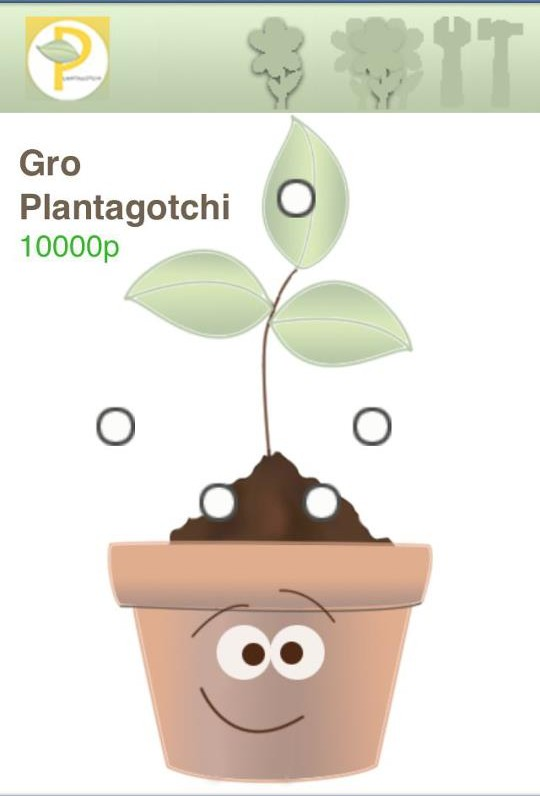
\includegraphics[width=0.5\textwidth]{img/introduction/plantagotchi.jpg}
\caption{Screenshot of Plantagotchi prototype}
\label{fig:scrshotplantagotchi}
\end{figure}

During the spring of 2013 we both took the course inf5790 \emph{Technology enhanced learning} and were introduced to the field of Computer Supported Collaborative Learning (CSCL). As we brought with us an idea of an application that pupils could use to collaboratively learn about a scientific domain, CSCL became the field where we could adapt theoretical perspectives and concepts, which set words to and explained our personal ideas and experiences. 

As mentioned, the starting point of this thesis was to do research on an actual working system, in an authentic environment. We therefore brought with us the ground idea from Plantagotchi and spent a lot of time improving it and developing a new working prototype. Furthermore, in October 2013 we got in touch with a school, and had a fully working plant monitoring system which we could test with real users in their natural setting. The focus in this thesis is therefore directed to this design experiment study performed in a high school biology class. We will however provide some background information about the decisions made while developing Monoplant. 


\section{Monoplant}
Plants live a slow life, they grow slowly and move slowly. Humans have no means of directly observe when a plant grow, but we are able to see that it has grown or bloomed. However, humans have the ability to use tools in order to make sense of the world, and we have created such a tool: Monoplant, which can help us see how plants evolve over time.

Monoplant is a monitoring system for plants, or rather humans who want to monitor their plants. It continuously gathers data about a plant's environment and makes the data available to the users via the Internet. One functionality is thereby to remotely monitor a plant and get instant data about temperature, humidity, light-level, soil moisture and even a picture of the plant. However, one of the main reasons for designing Monoplant, was that we wanted to see how plants develop over time, or in biological terms their ontogenetic development. Hence we tried to combine readings over time to see if we were able to observe if some of the variables affected the plant physically. The first step became to merge the images taken into a time-lapse video. This made it possible to see a plant's physical development throughout a day in a matter of seconds. In order to link this with the variables from the environment, we had to connect each image in the video to it's corresponding data reading. This is done by presenting a graph together with the time-lapse video and marking the point in the graph which corresponds to the current image in the video (see figure~\ref{fig:scrshotgraphlapse}). Thus we are connecting \emph{visible} changes of the plant (i.e., the video) to \emph{invisible} changes in the environment (e.g., soil moisture and humidity levels).


\begin{figure}
	\centering
	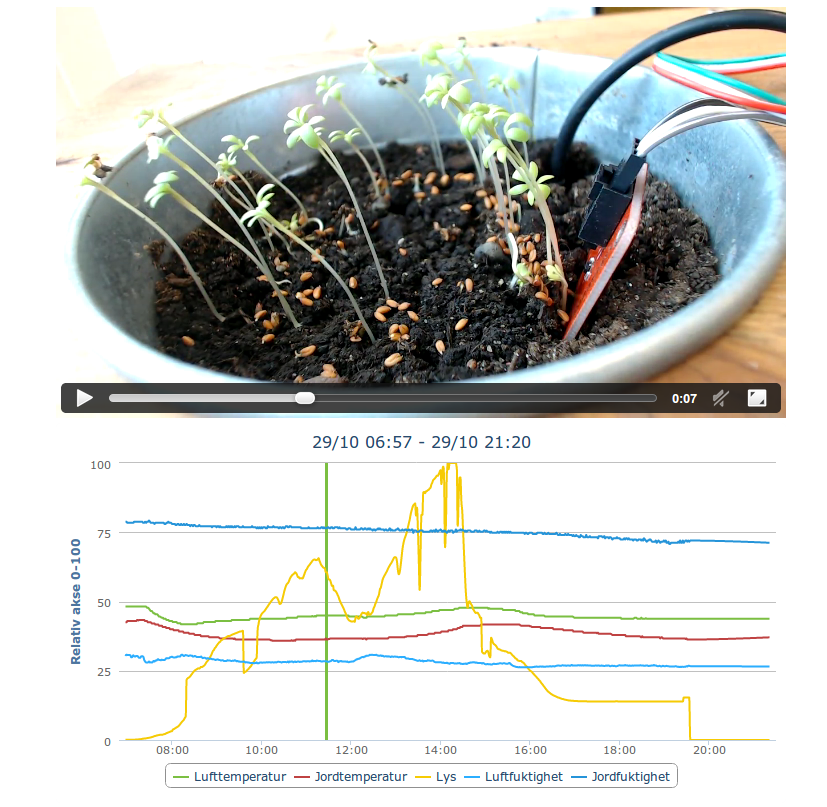
\includegraphics[width=\textwidth]{img/introduction/graphlapse.png}
	\caption{Screenshot of timelapse and graph}
	\label{fig:scrshotgraphlapse}
\end{figure}

%Maybe write something about how this is generic, but that in this thesis we have chosen to focus on how it can be used in learning.

\section{Research questions}
%place our focus in the CSCL field
As mentioned, the overall theme of this thesis will be how students can use Monoplant in their scientific inquiry when learning about photosynthesis in a biology class. This will be investigated through an analysis of a study performed the autumn of 2013. In order to address this broad theme we will try to answer four research questions. The first question is: 


\begin{noindlist}
\item \emph{"What characterizes the students’ inquiry in interaction with Monoplant?"}\\
This will naturally adress the characteristics of the students' actions and interactions during their work with Monoplant. The first question will also be elaborated through the next three questions.
\item \emph{"How does Monoplant, by presenting photosynthesis differently from the text book, support the inquiry process?"}\\
This question is indicating that there is a difference between the representation of photosynthesis in the school textbook and in Monoplant. To answer this we will address these differences, and discuss what implications they have in the students' inquiry process.
\item \emph{"In what way is scaffolding operationalized in the environment?"}\\
For this question to make sense, we need to introduce the theoretical concept of \emph{scaffolding} and put it in a broader context of instructional theory. This will be elaborated later in the thesis, but for now we can call it training wheels. We will look at how the teacher and Monoplant help the students in their inquiry process.
\item \emph{"How does the institutional setting frame the students inquiry process?"}.\\
As the study took place in a school setting, we wanted to look at how the social practices within school affected the inquiry process.
\end{noindlist}


\section{Thesis outline}
%scientific backgroud 
%technical background
%theory
%empirical & method
%data and analysis
%discussion
%concluding remarks
We will now present an outline for this thesis, providing an overview of the content as well as the structure. 

\subsubsection*{Chapter 1 - Introduction}
The introduction presents our personal and professional motivations for writing this thesis, a brief introductions to Monoplant followed by the research questions, and lastly this "readers guide".

\subsubsection*{Chapter 2 - Scientific background}
This chapter is an introduction to photosynthesis and thereby the scientific language within the domain. The introduction represents what the students in our case are supposed to learn in \emph{Biology 2}. It is provided as a tool to understand what we mean later in the thesis when using domain specific terms such as \emph{"light dependent reaction"}, \emph{"excited"} or \emph{"chlorophyll molecules"}.

\subsubsection*{Chapter 3 - Technical architecture and programming}
%The application is divided into three logical units: data collection, data processing and database, and user interface. In the following sections these units will be explained further. 
A major part of the work done was to design and build Monoplant. In this chapter we will describe Monoplant's architecture and address some of the technical concerns we met during the development process. We will introduce \emph{Raspberry Pi}, \emph{Arduino}, \emph{Ruby on Rails}, \emph{REST} and other frameworks and tools used to build Monoplant.

\subsubsection*{Chapter 4 - Theoretical perspective and concepts for analysis}
%In this chapter we will lay forth the theoretical perspective and theoretical concepts we will apply in this thesis. First we will introduce the \emph{sociocultural perspective} and highlight some key points including \emph{institutional practices}, \emph{zone of proximal development} and \emph{scaffolding}. Further we will look at \emph{multiple external representations} and lastly the concept and method of \emph{Inquiry learning}.

In this chapter we will present the sociocultural perspective, which will be used throughout this thesis. We will also introduce the theoretical concepts: \emph{spontanous and scientific concepts}, \emph{zone of proximal developement (ZPD)}, \emph{scaffolding}, \emph{multiple external representations (MER)}, \emph{institutional settings}, \emph{inquiry learning} and \emph{misconceptions}. We will make an account for our interpretation of these concepts as we will use them later in the thesis to help answer our research questions. 

\subsubsection*{Chapter 5 - Empirical setting and method}
%In this chapter, we will present the empirical setting and methods used in this thesis. First we will describe the empirical setting in which the data collection took place. Then we will proceed to present the methods for gathering data with a description of the technicalities of the data. Lastly, we will describe the procedures for selection and analysis of data.

Throughout October 2013 we gathered data for this thesis. In this chapter we will introduce \emph{design based research} and describe the empirical setting in which this data gathering took place. We will also describe the methods used for collecting the data and how we chose to use those methods. Lastly we will explain how we approached, selected and made sense of the data once the data collection was done. 

\subsubsection*{Chapter 6 - Data and analysis}
%In this chapter we will present the findings from our case study with a focus on themes relevant to our research questions. Each of the themes contain at least one excerpt with a context description, excerpt from the transcript, and an analysis of the unfolding events.
Here we will present the main findings from our study. The chapter contains 10 data extracts, which is presented one by one. First by a context description, then a data transcript and finally a clarification and analysis of what happened. 

\subsubsection*{Chapter 7 - Discussion}
%In this chapter we discuss our research questions by contextualizing our findings according to the theoretical concepts introduced earlier. As an overall theme we look at the inquiry process of the students in interaction with Monoplant. This will be showed through 4 sections, the first being about the inquiry process itself. Next we will discuss how multiple external representations support the inquiry process of the students. Then how scaffolding is instantiated in the environment, and finally how the institutional setting frame the students' inquiry process.
In this chapter we will discuss our research questions by applying the theoretical concepts introduced in chapter 4. Our first research question \emph{"What characterizes the students’ inquiry in interaction with Monoplant?"} will be the overall theme of this chapter, but all four of the questions will be addressed.

\subsubsection*{Chapter 8 - Concluding remarks}
Our concluding remarks will provide the reader with an overview of how we approached this thesis and a review of our main findings according to the research questions. Lastly we will present shortcomings and suggestions for further work.
 %!TEX root = ../document.tex
\chapter{Scientific background}
\label{cha:scientificbg}
In this chapter we will first give a rudimentary introduction to photosynthesis as it is described in the curriculum for Biology 2 \citep{bios}. Then proceed to some monitoring and automated systems, which will lead to the next chapter, an introduction to Monoplant and its technical specifications.

\section{Photosynthesis}
The variables that we monitor in our application are directly linked to the precondition of all life, photosynthesis. During this process plants transform energy from light to chemical energy in the form of e.g., glucose and starch. As most organisms are not able to make use of light energy directly, plants are a necessity for producing energy that other organisms can transform. The equation for photosynthesis is written as: \ce{(CO2)n + (H2O)n + photons -> (CH2O)n + (O2)n}, which means that carbon dioxide, water and light transform to glucose and oxygen.  

Photosynthesis consists of two main parts: the light-dependent reaction, and the light-independent reaction. The light-dependent reaction, as the name implies, occur only in the light. The light-independent reaction occurs both in the light and dark, but does not rely on energy from photons.  

\begin{figure}
\centering
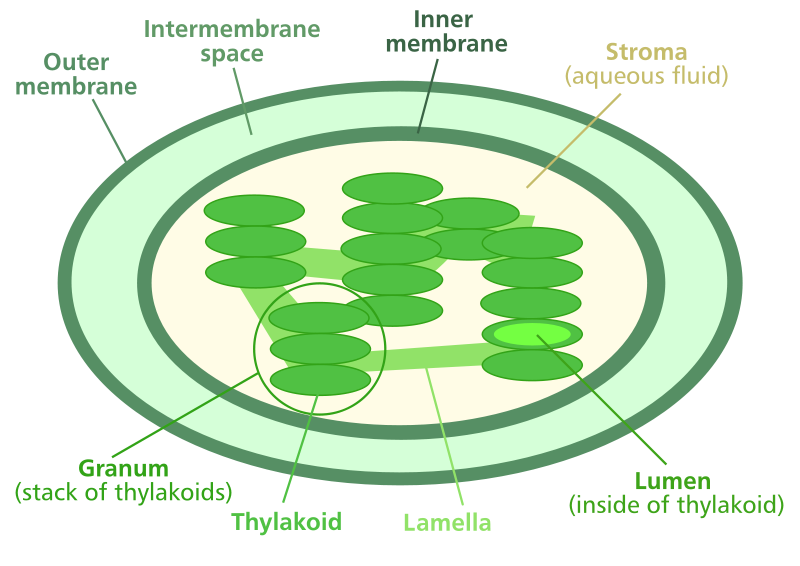
\includegraphics[width=0.8\textwidth]{img/photosynthesis/Chloroplast_diagram.png}
\caption{Illustration of a chloroplast molecule \citep{wiki:chloroplast}}
\label{fig:chloroplast}
\end{figure}

\subsection{Light-dependent reaction}
The light-dependent reaction consists of two different photosystems (photosystem 1 and photosystem 2) creating adenosine triphosphate (ATP) and nicotinamide adenine dinucleotide phosphate (NADPH) molecules for the light-independent reactions. Both systems are located in the thylakoid membrane inside the chloroplast organelles (see fig.~\ref{fig:chloroplast}). In the process, photosystem 2 precedes photosystem 1 as photosystem 1 was discovered first. 

\subsubsection*{Photosystem 2}
In photosystem 2, antenna-complexes consisting of pigments, proteins and enzymes absorb light of different wavelengths and transfer the energy to chlorophyll molecules \citep{bios}. The energy leads to electrons jumping to an orbit lying further from the nucleus, making the atom excited. This makes the atom unstable, and a perfect candidate for giving away its electrons to electron-acceptors in an electron-transport chain.

Since the chlorophyll loses two of its electrons in the process, it gets positively charged and need to find new electrons to be able to absorb photons again. This happens by taking two electrons from a water molecule absorbed by the plant's roots, which then gets split into \ce{2H+} and \ce{1/2O2} \citep{bios}. The oxygen dissolves in the air, while the hydrogen protons are “trapped” on the inside of the thylakoid membrane (lumen). This makes the lumen positively charged relative to the stroma, which enables generation of ATP-molecules from ADP- and P-molecules. 

\subsubsection*{Photosystem 1}
Photosystem 1 consists of the same parts as photosystem 2, but instead of splitting water molecules, it receives two electrons from the electron transport chain in photosystem 2. These electrons gets transferred out in the stroma, and are then tied together with an h+-proton and NADP+ to produce NADPH.

\begin{figure}
\centering
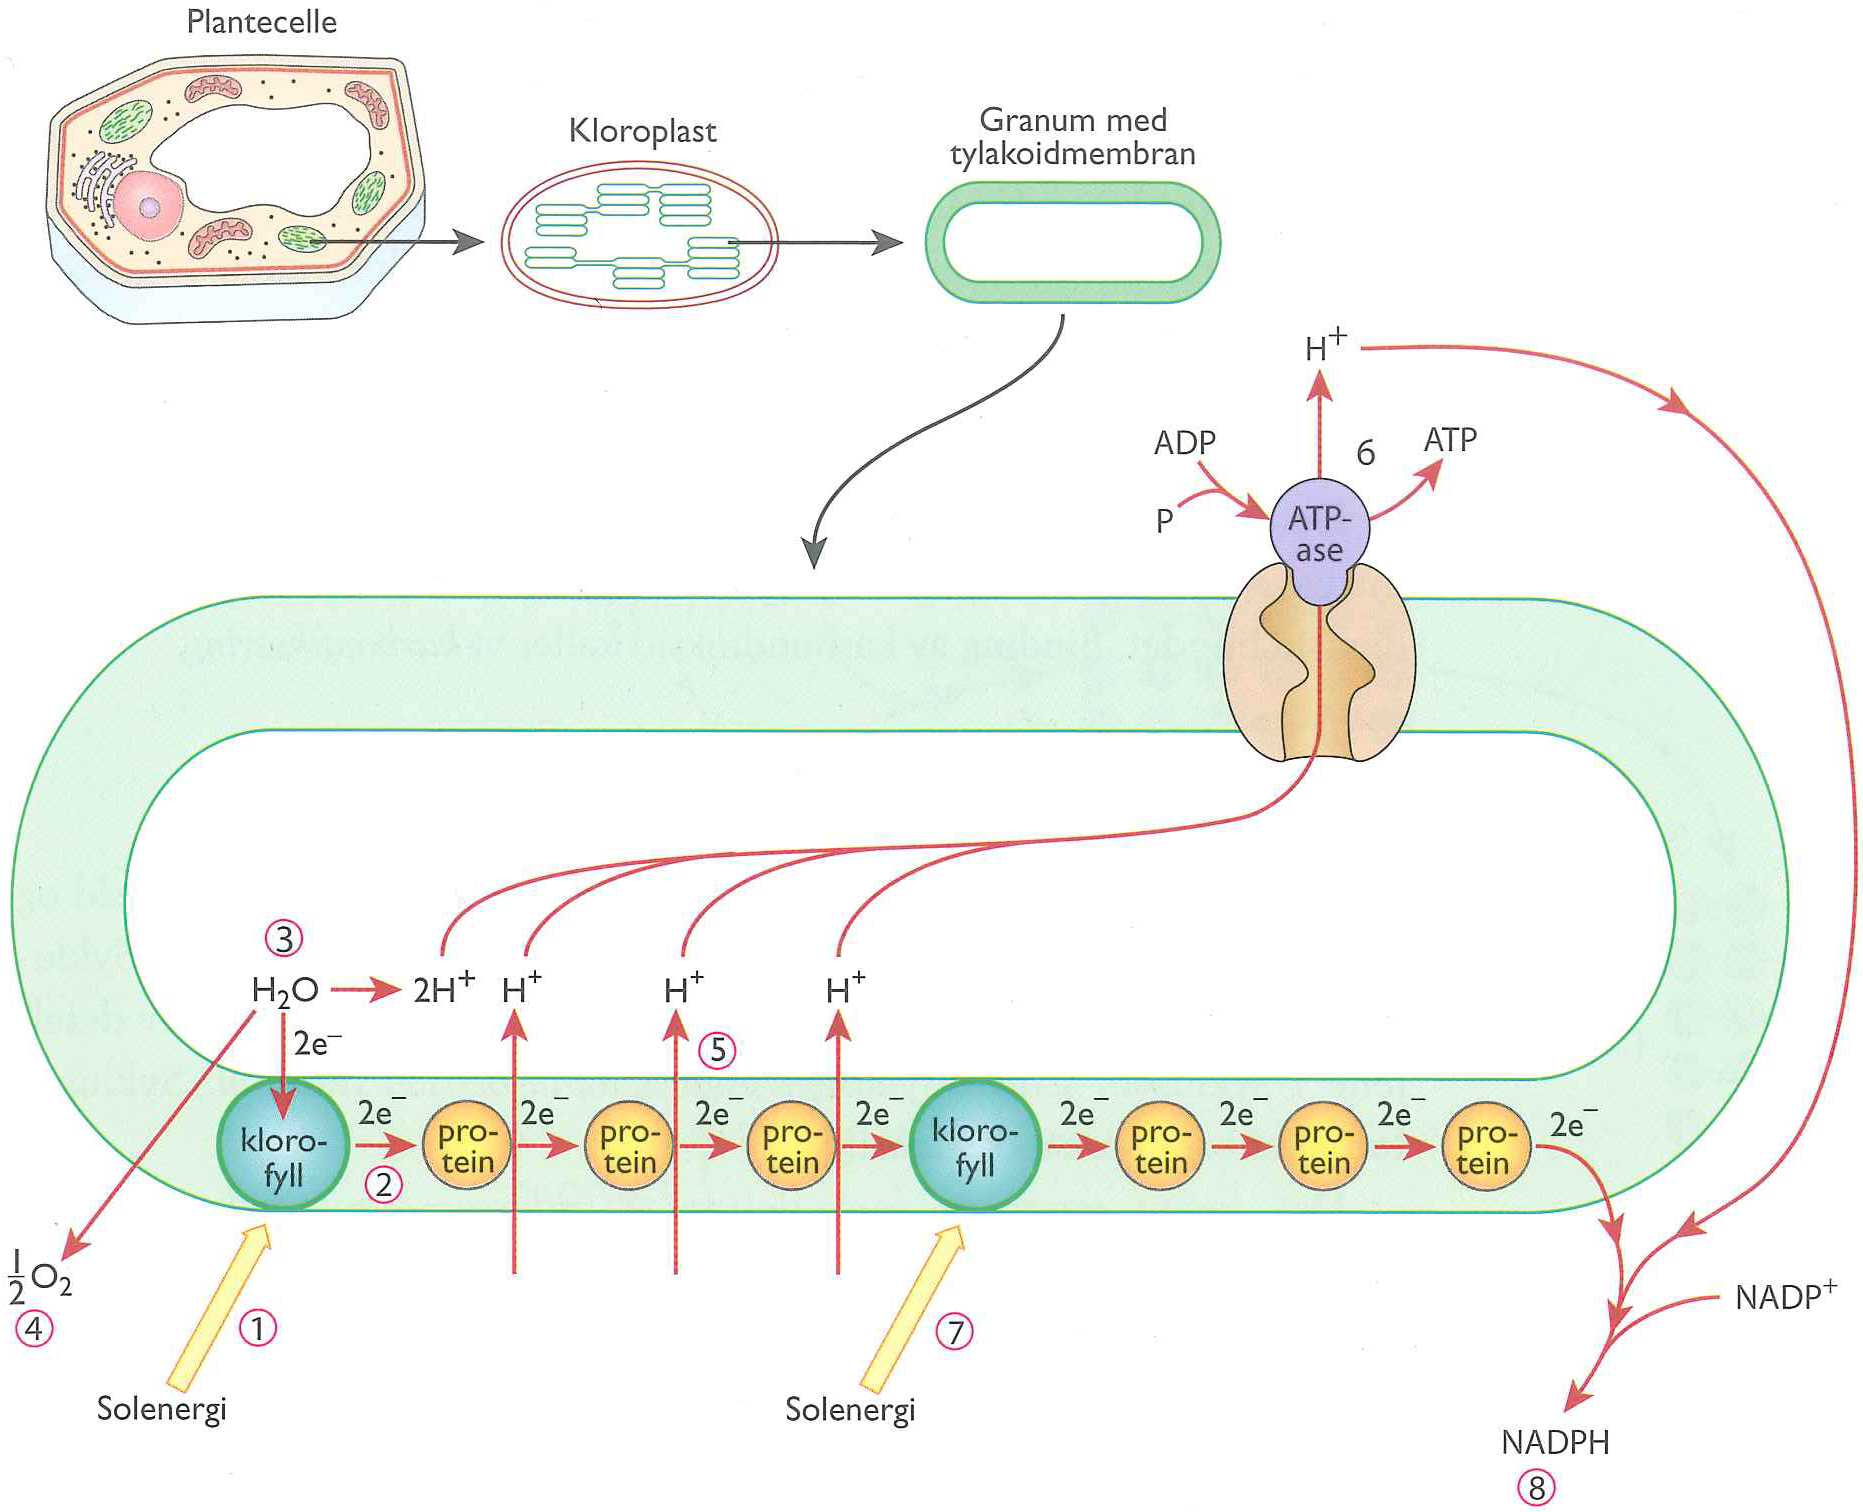
\includegraphics[width=\textwidth]{img/photosynthesis/light_dependent.png}
\caption{Illustration of PS1 and PS2 \citep{bios}}
\label{fig:photosystem}
\end{figure}

\subsection{Light-independent reaction (Calvin-cycle)}
This reaction works as a “sugar-factory”, collecting carbon dioxide and hydrocarbon in many cycles to make glucose. The process takes place in the stroma (see fig.~\ref{fig:chloroplast}), and requires the NADPH and ATP generated in the light-dependent reaction \citep{bi2}. 

The glucose produced can be used to generate other organic compounds such as other carbohydrates (e.g., starch and cellulose), proteins and lipids, depending on what the plant needs.

\subsection{External factors}
Many external factors affect the photosynthesis in plants. As photosynthesis is a relatively inefficient process, using only 8-10\% of the energy in sunlight, much research has gone into increasing photosynthesis to achieve greater conversion rates \citep{kirschbaum2011does}. The factors of significance are \citep{bios}:
\begin{itemize}
\item \ce{CO2} levels
\item Temperature
\item Light intensity and wavelength
\item Water
\end{itemize}
Each of these factors may be a limiting factor, or stressfactor, not enabling photosynthesis to reach its full potential. 

\subsubsection{\ce{CO2} levels}
\ce{CO2} is used in the light-independent reaction for making glucose. The atmosphere contains approximately 0.038\% \ce{CO2}, while the air in e.g., a classroom would most likely contain slightly higher values due to a high concentration of students exhaling \ce{CO2}. In a greenhouse \ce{CO2} levels can get too low, due to a high concentration of plants consuming \ce{CO2} and outputting \ce{O2}. The optimal concentration for most plants is between 0.015\% and 0.05\% \citep{bios}. 


\begin{figure}
        \centering
        \begin{subfigure}[b]{0.45\textwidth}
                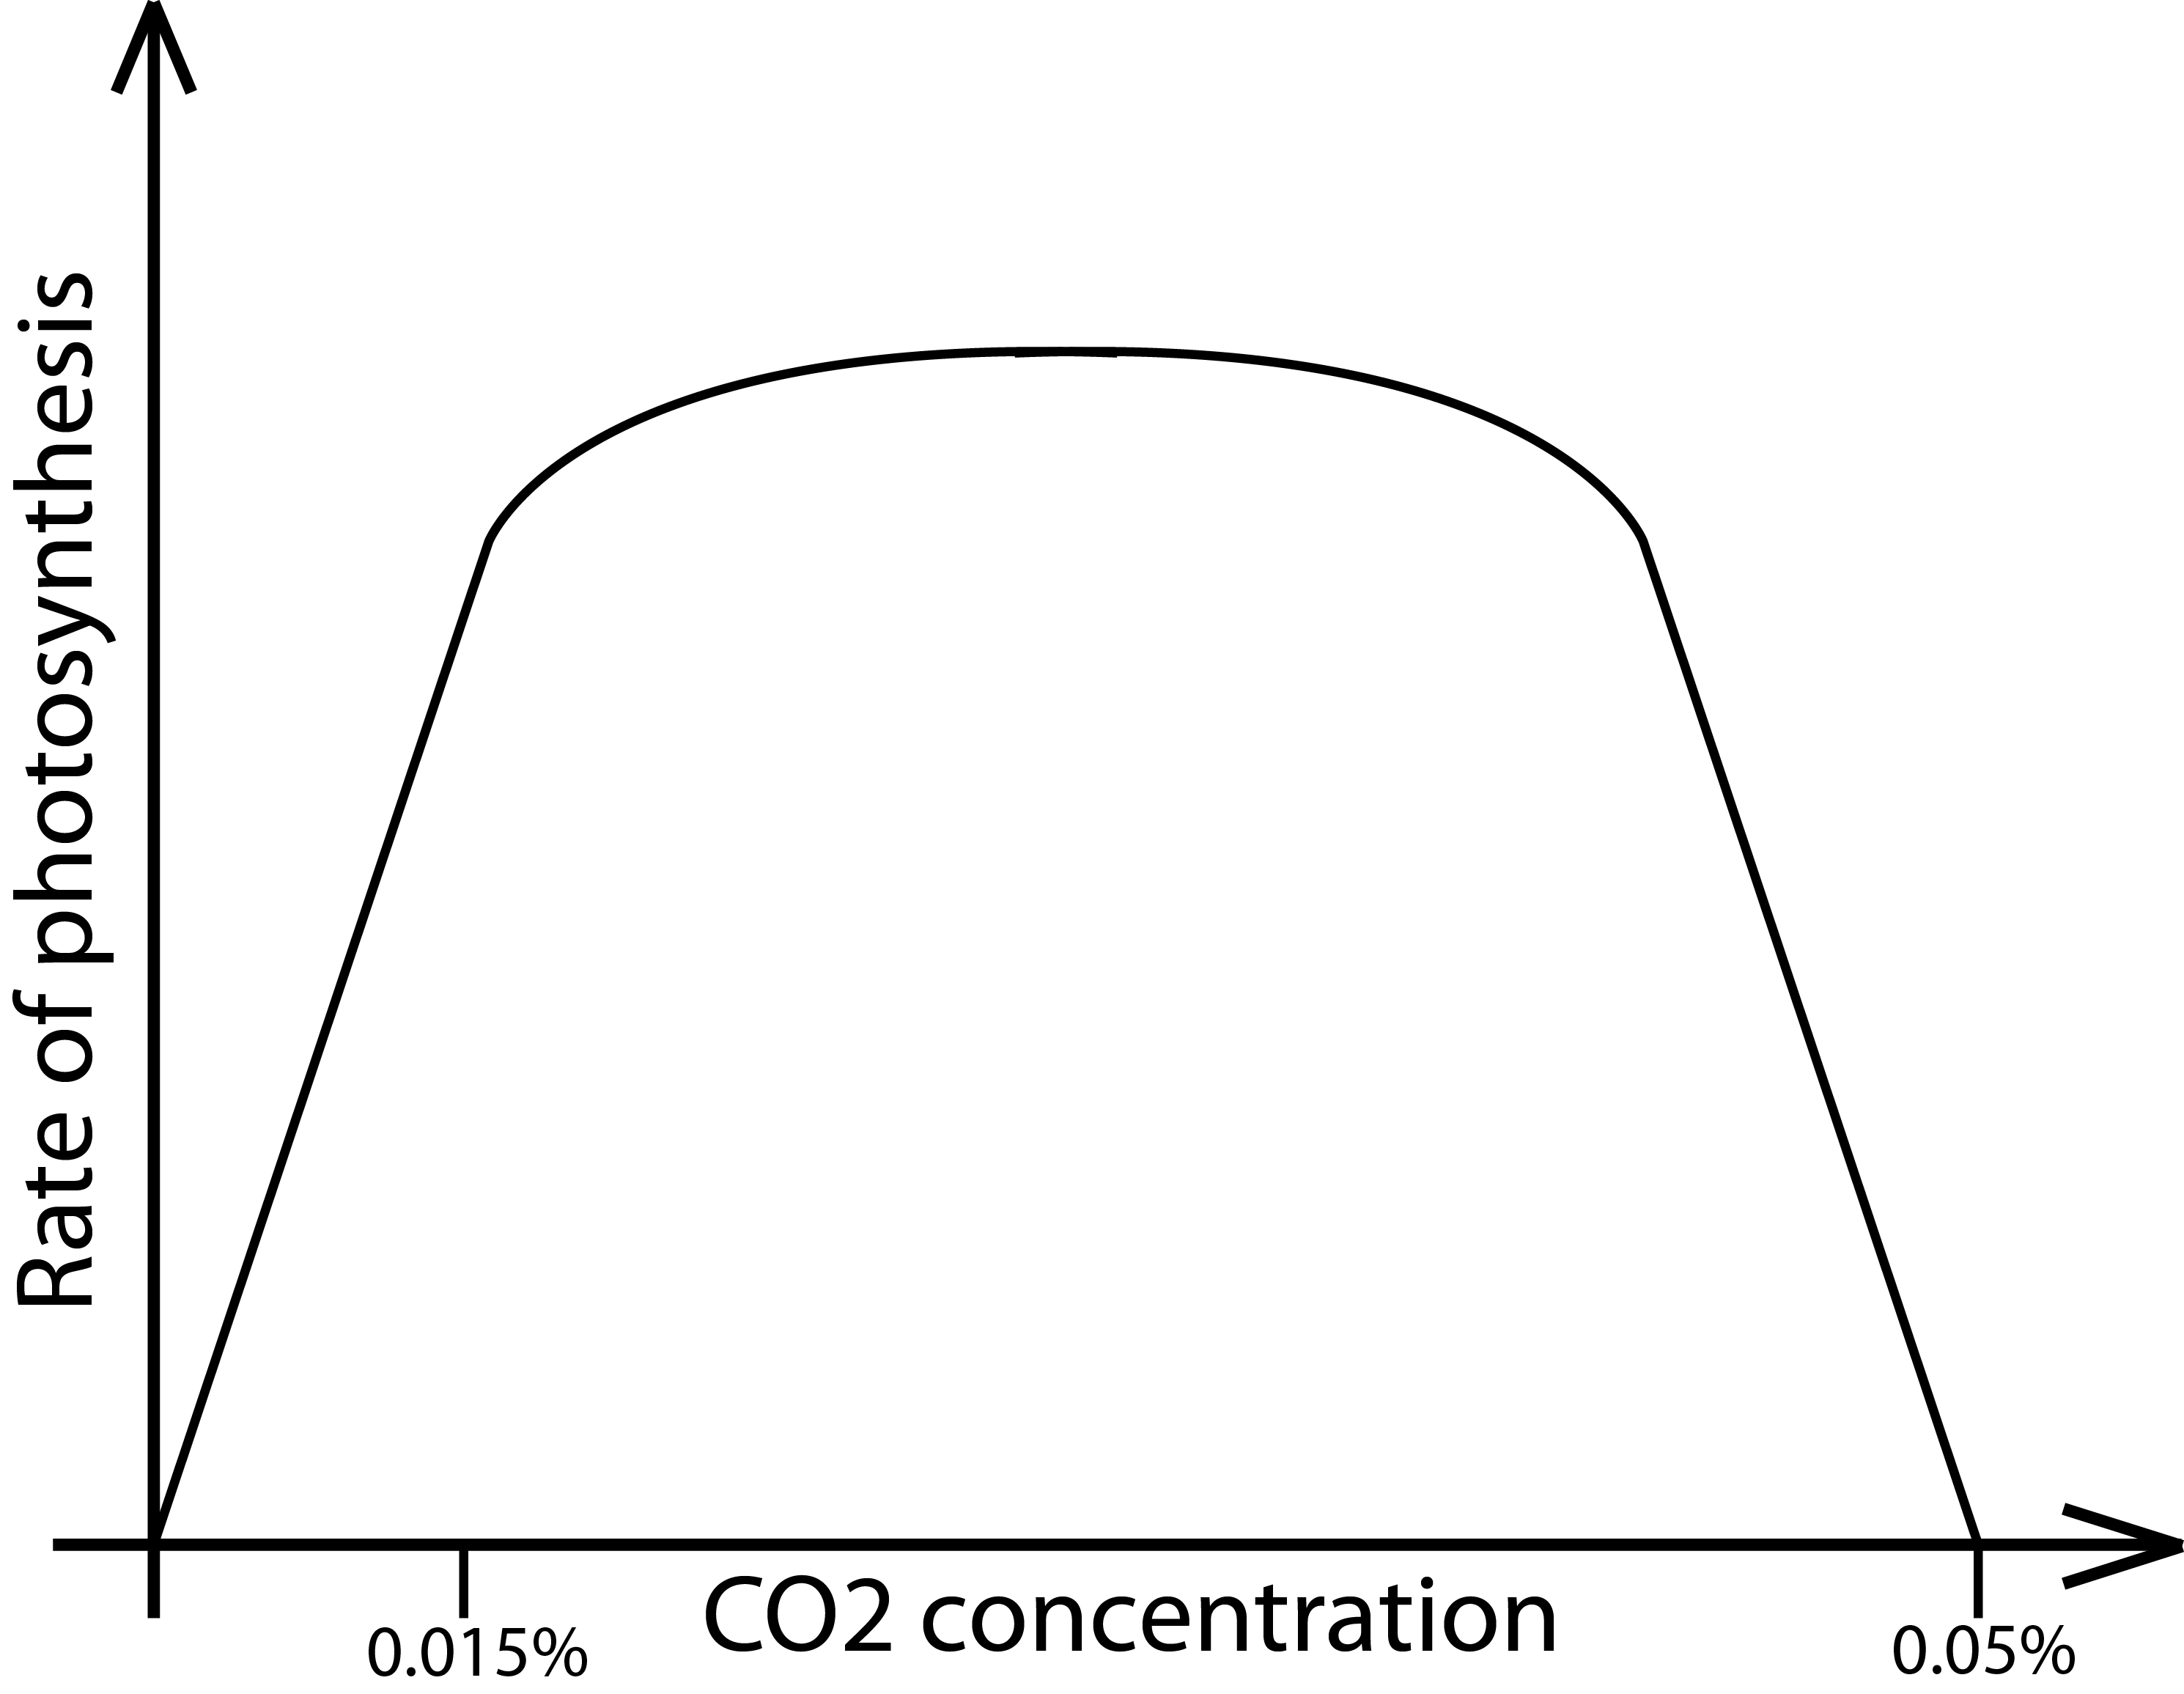
\includegraphics[width=\textwidth]{img/photosynthesis/co2.png}
                \caption{Effect of \ce{CO2} levels on photosynthesis}
                \label{fig:co2levels}
        \end{subfigure}
        ~~
        \begin{subfigure}[b]{0.45\textwidth}
                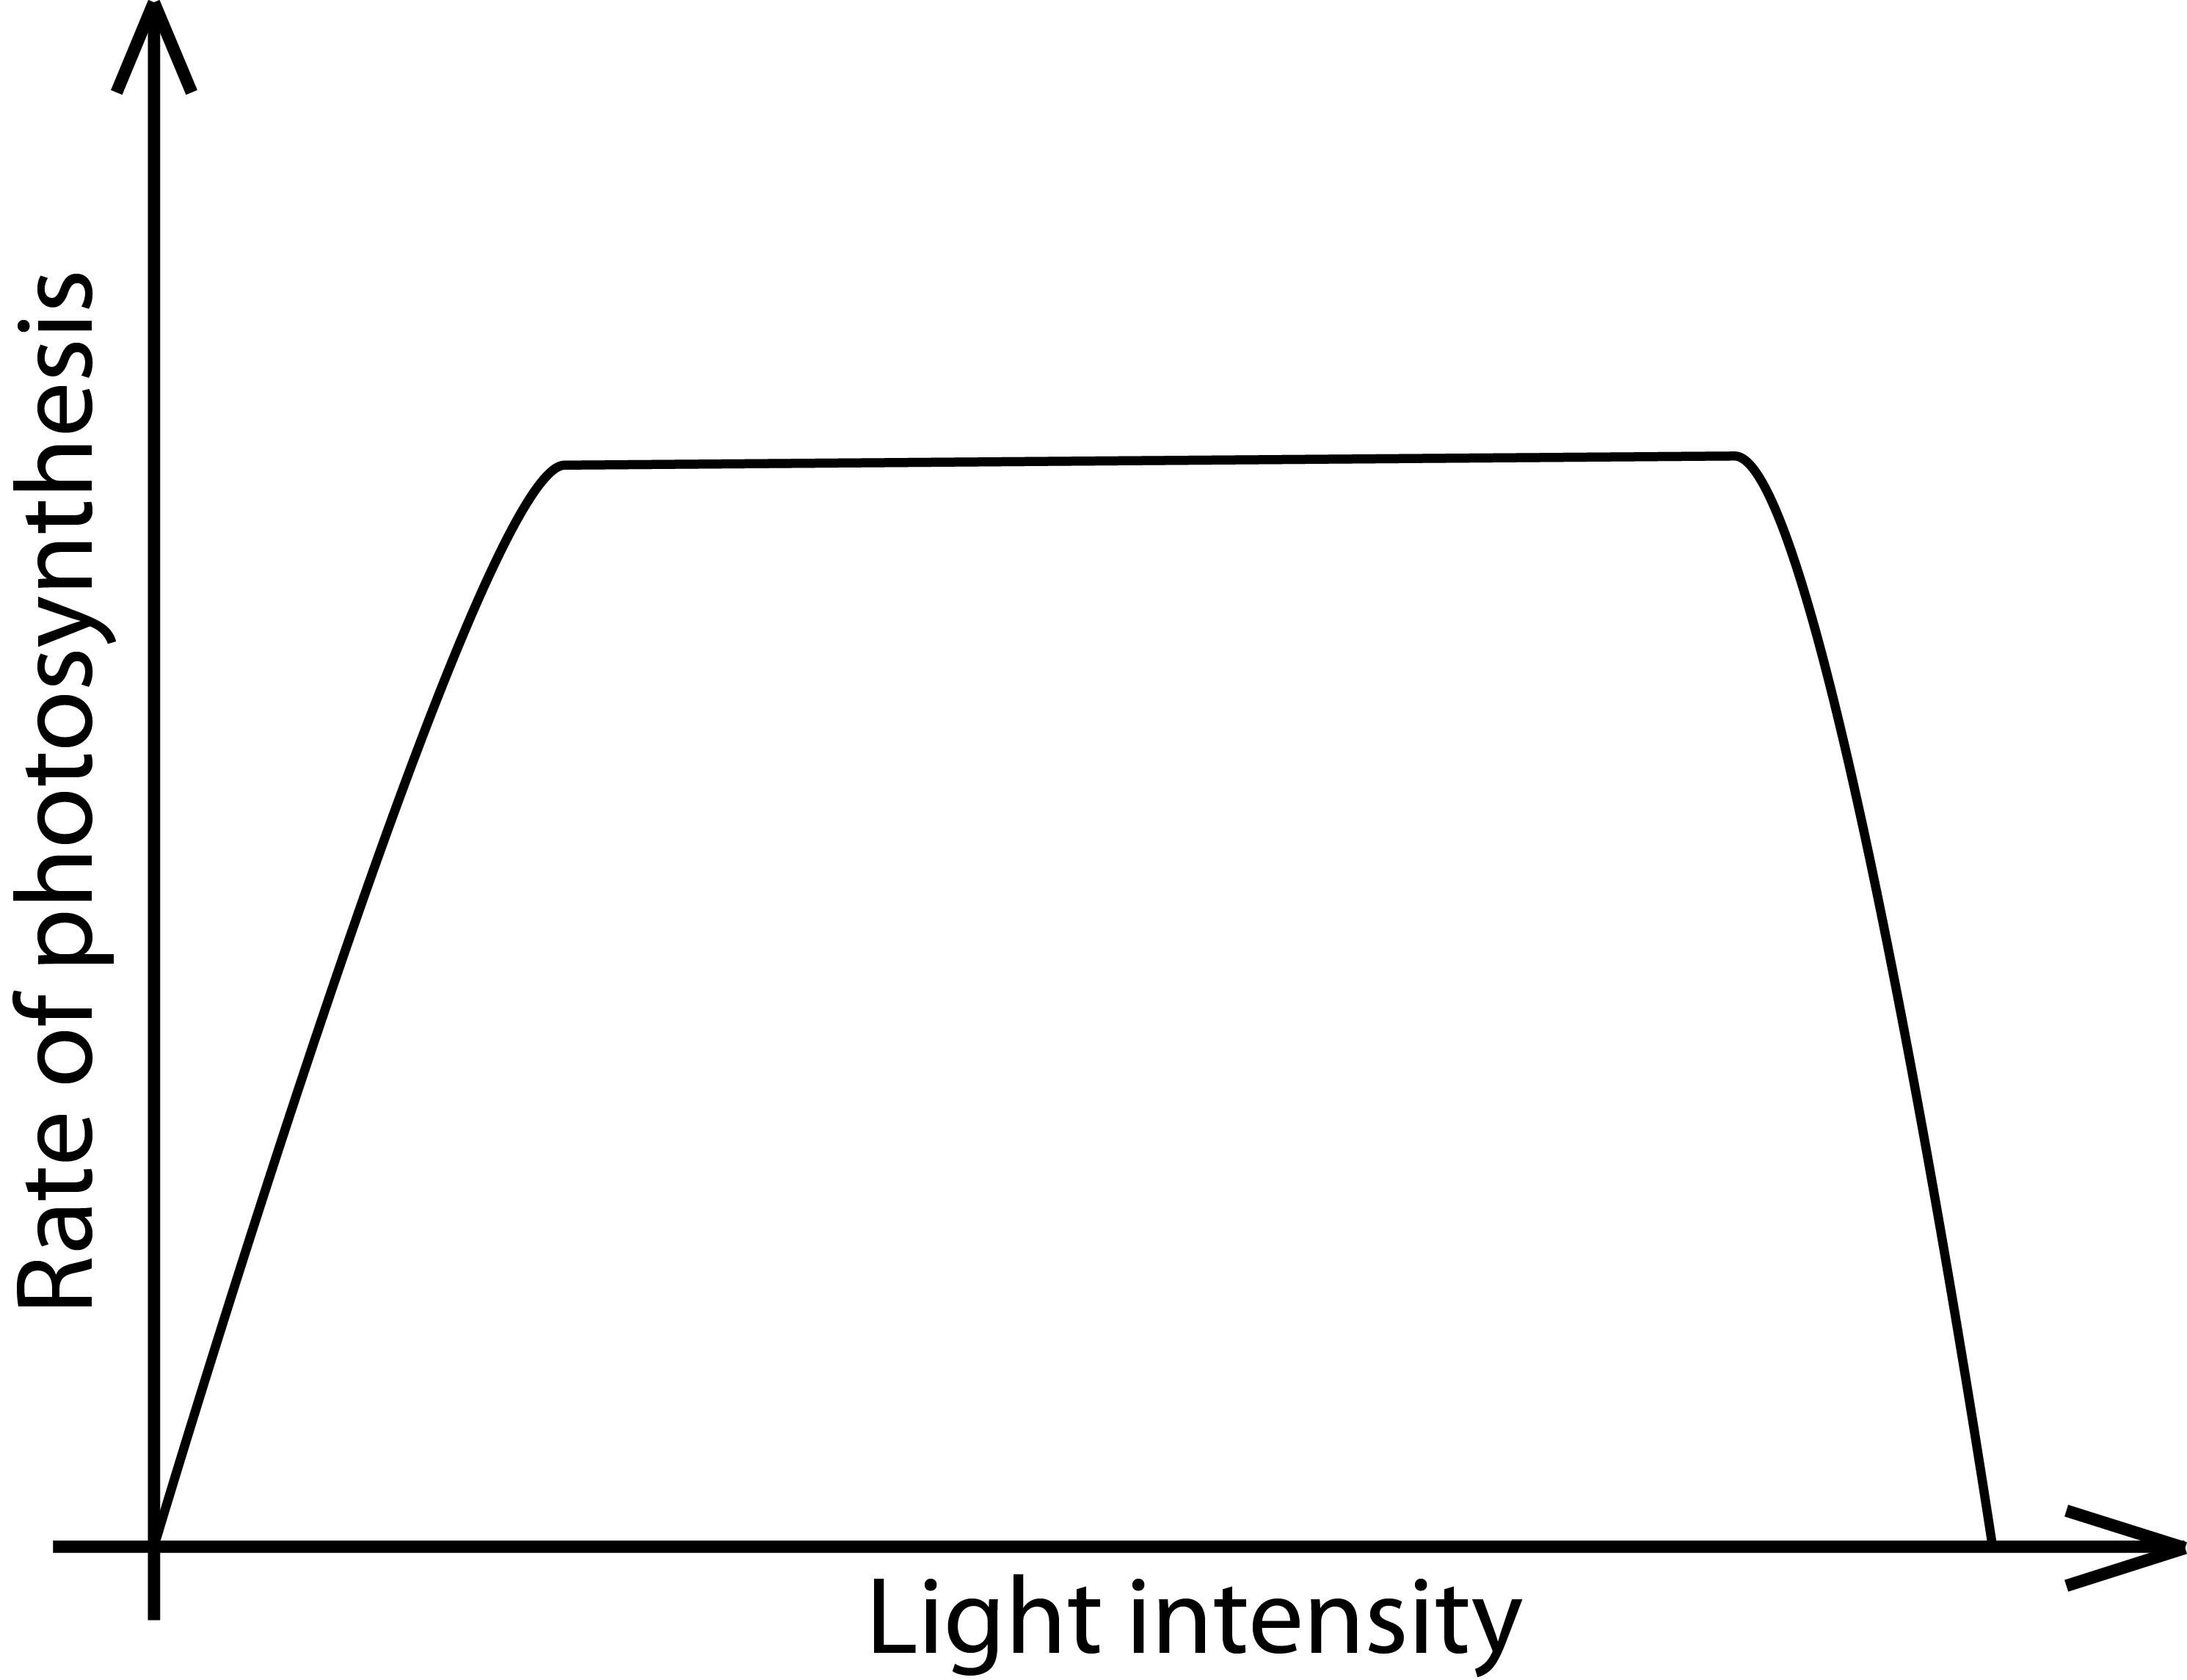
\includegraphics[width=\textwidth]{img/photosynthesis/light_intensity.png}
                \caption{Effect of light intensity on photosynthesis}
                \label{fig:lightintensity}
        \end{subfigure}
       
\end{figure}

\begin{figure}
\centering
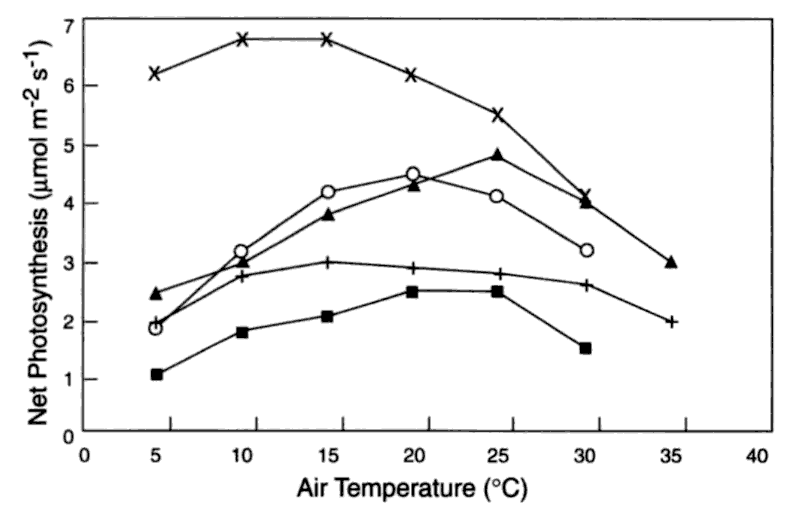
\includegraphics[width=0.75\textwidth]{img/photosynthesis/temperature_new.png}
\caption{Effect of temperature on photosynthesis. Species:
 \textit{\ensuremath{\blacktriangle} Pinus Taeda},  
\textit{\ensuremath{\bigcirc} Pinus Strobus}, 
\textit{\ensuremath{+} Pinus Sylvestris}, 
\textit{\ensuremath{\blacksquare} Picea Engelmanii}, 
\textit{\ensuremath{\times} Pinus Ponderosa}
\citep{hollinger1995external}
}
\label{fig:temperature}
\end{figure}

\subsubsection{Temperature}
All enzymes have an optimal temperature during which they function best \citep{bios}. This temperature may vary from species to species as plants grow in different climates, altitudes and seasons. If the temperature is too low or too high, the molecular structure of the enzymes may be destroyed.

\subsubsection{Light intensity and wavelength}
The different pigments in the light dependent reaction absorb light of wavelengths from mainly 400nm to 700nm. Chlorophyll b for instance absorbs blue light (450nm). If a plant with a high concentration of chlorophyll b is not given light of this wavelength, the electrons would not be excited and the reaction in photosystem 2 would not start.

Light intensity also plays a role in this reaction. In low light conditions, there is not enough energy available to excite the chlorophyll molecules, in order to move electrons as needed in PS2. In optimal light conditions, the production is light-saturated meaning that all the chlorophyll molecules are exciting electrons. In too strong light conditions, the chloroplasts may burn out from the heat and die.  

\begin{figure}
        \centering
        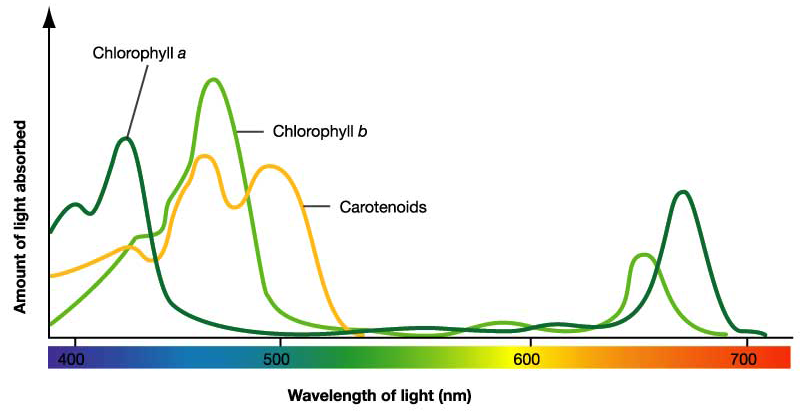
\includegraphics[width=0.8\textwidth]{img/photosynthesis/absorption-spectrum.png}
        \caption{Wavelengths of light absorbed by different pigments}
        \citep{uicbiology}
        \label{fig:wavelengthabsorbtion}
\end{figure}

\subsubsection{Water}
Water is used in both the light-dependent and light-independent reactions, but is seldom a limiting factor. If water-levels are low and the evaporation-rate is high, most plants will close the leaves to minimize water-loss. This makes the plant unable to absorb \ce{CO2} and photons, which leads to plant reduction \citep{bi2}. Water shortage is only a problem in itself when the plant's cells dries out, leading to the stem and tissue collapsing. 


% \section{Koubachi} %Dette er noe dritt! fuck Koubachi. jævla sveitsere
% \begin{figure}
%         \centering
%         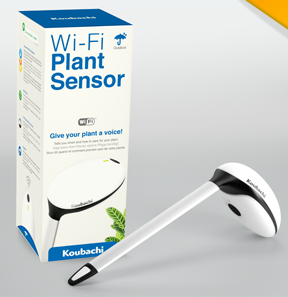
\includegraphics[width=0.4\textwidth]{img/koubachi/sensor.png}
%         \caption{Koubachi}
%         \label{fig:koubachi}
% \end{figure}

% Koubachi is a commercial plant monitoring system developed by a company by the same name. The functioning steps of Koubachi is divided in 3: 1.)\emph{Measure}, 2.) \emph{Analyze} and 3.) \emph{Display}. This is done through a sensor unit, the \emph{Koubachi Plant Care Engine (PCE)} and user interfaces in form of a web application and an iOs application \citep{koubachi}. As seen in figure~\ref{fig:koubachidata}, the sensor unit measures soil moisture, temperature and light. The web interface displays the last of the transmitted readings. The koubachi transmits data once every 24 hours in order to save battery life. It does however read data every tenth minute, so the PCE has access to how the environment change over the span of each day.

% The PCE is basically an API with the functionality of storing data from sensors, analyzing the data and distributing data and instructions on how and when to care for the plant. Based on plant care models developed by biologists through greenhouse experiments, the PCE can determine the needs of any plant species. Thus, combining the data gathered by the sensor unit with the plant care model, Koubachi provides notifications about how and when to care for your plant. An example of this can be seen in figure~\ref{fig:koubachigraph}, where a graph of light measurements the preceding week i displayed together with a note that \emph{Gretches has too much shade} (Gretches beeing the name of the plant). Apart from obvious technical differences, this seems to be the main divergence from Monoplant; Koubachi is not only presenting data, it is also providing an opinion if the plant is comfortable or not, even suggesting measures for care taking.

% \begin{figure}
%         \centering
%         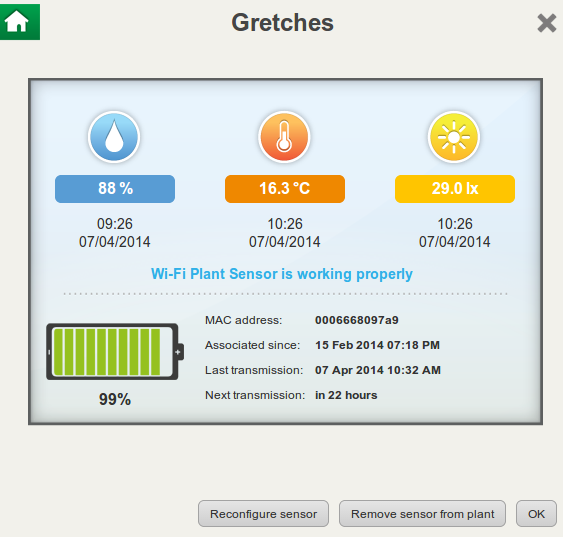
\includegraphics[width=0.8\textwidth]{img/koubachi/instantdata.png}
%         \caption{Last data from web interface}
%         \label{fig:koubachidata}
% \end{figure}

% \begin{figure}
%         \centering
%         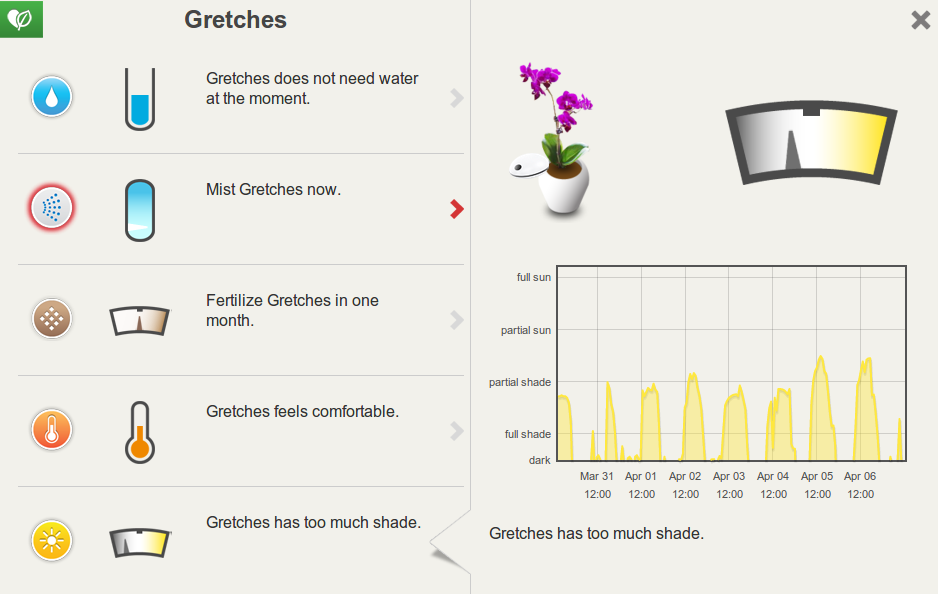
\includegraphics[width=0.8\textwidth]{img/koubachi/lightgraph.png}
%         \caption{Light graph from web interface}
%         \label{fig:koubachigraph}
% \end{figure}


 %!TEX root = ../document.tex
\chapter{Technical architecture and programming}
In this chapter we will present the technical aspects of our learning tool, Monoplant. We will explain the rationale for the design choices made, and go into detail on some of the more advanced parts of the system. We will not give an in-depth explanation of all the technicalities, but rather present an overview to give the reader some background to understand the learning opportunities built into the system. First we will give a short introduction of some related applications, then we present Monoplant based on its architectural structure. First addressing the data collection, then data processing and storage, and finally the user interface.

\section{Related applications}
When starting our work with Monoplant, a review of existing technology was done. While there is some commercial plant monitoring systems, the major part of existing projects where characterized by the "do it yourself"-style (DIY). The latter involved use of prototype platforms such as Arduino, where the makers provided instructions for how people could make their own version of their system. Projects reviewed included twittering plants, plants making phone-calls, self-watering plants and gardening Arduinos \citep{botanicalls,selfwater,garduino}. All the DIY projects where focused on responding to variable changes around the plant, and can therefore be categorized as automated systems. 

The commercial products reviewed where Koubachi and Twine \citep{koubachi,twine}. Twine being a monitoring system for usage in the home and Koubachi a plant monitoring system with a focus on helping people take care of their plants. The systems reviewed proved that there is an interest for plants and for using technology to bridge the gap in human-plant interaction. However, the tools are not concerned with learning, and are mostly making use of 1-3 environmental variables, paying no attention to capturing visual images of plants. Monoplant is therefore a more complex system, and the systems reviewed did not inform our design to any large degree.

% \section{Koubachi} %Dette er noe dritt! fuck Koubachi. jævla sveitsere
% \begin{figure}
%         \centering
%         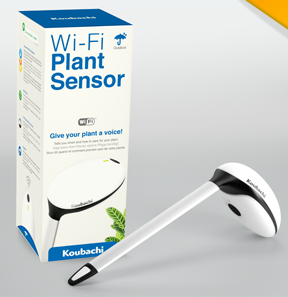
\includegraphics[width=0.4\textwidth]{img/koubachi/sensor.png}
%         \caption{Koubachi}
%         \label{fig:koubachi}
% \end{figure}

% Koubachi is a commercial plant monitoring system developed by a company by the same name. The functioning steps of Koubachi is divided in 3: 1.)\emph{Measure}, 2.) \emph{Analyze} and 3.) \emph{Display}. This is done through a sensor unit, the \emph{Koubachi Plant Care Engine (PCE)} and user interfaces in form of a web application and an iOs application \citep{koubachi}. As seen in figure~\ref{fig:koubachidata}, the sensor unit measures soil moisture, temperature and light. The web interface displays the last of the transmitted readings. The koubachi transmits data once every 24 hours in order to save battery life. It does however read data every tenth minute, so the PCE has access to how the environment change over the span of each day.

% The PCE is basically an API with the functionality of storing data from sensors, analyzing the data and distributing data and instructions on how and when to care for the plant. Based on plant care models developed by biologists through greenhouse experiments, the PCE can determine the needs of any plant species. Thus, combining the data gathered by the sensor unit with the plant care model, Koubachi provides notifications about how and when to care for your plant. An example of this can be seen in figure~\ref{fig:koubachigraph}, where a graph of light measurements the preceding week i displayed together with a note that \emph{Gretches has too much shade} (Gretches beeing the name of the plant). Apart from obvious technical differences, this seems to be the main divergence from Monoplant; Koubachi is not only presenting data, it is also providing an opinion if the plant is comfortable or not, even suggesting measures for care taking.

% \begin{figure}
%         \centering
%         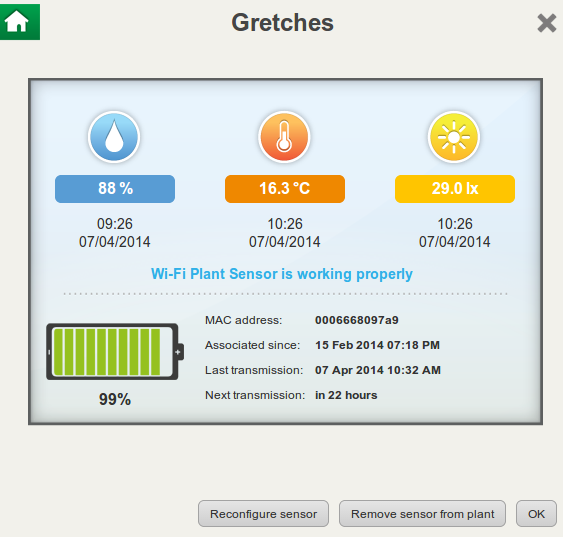
\includegraphics[width=0.8\textwidth]{img/koubachi/instantdata.png}
%         \caption{Last data from web interface}
%         \label{fig:koubachidata}
% \end{figure}

% \begin{figure}
%         \centering
%         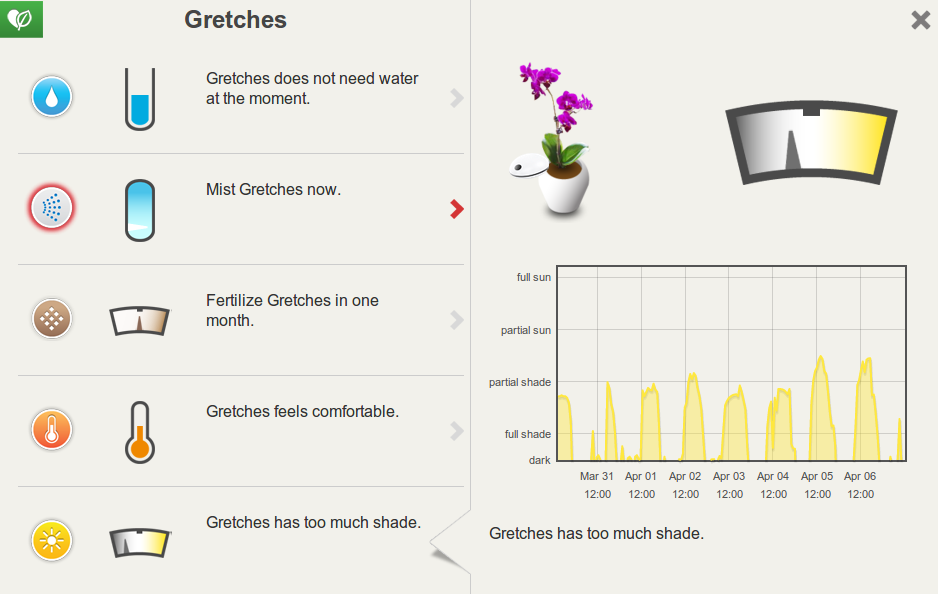
\includegraphics[width=0.8\textwidth]{img/koubachi/lightgraph.png}
%         \caption{Light graph from web interface}
%         \label{fig:koubachigraph}
% \end{figure}


\begin{figure}
\centering
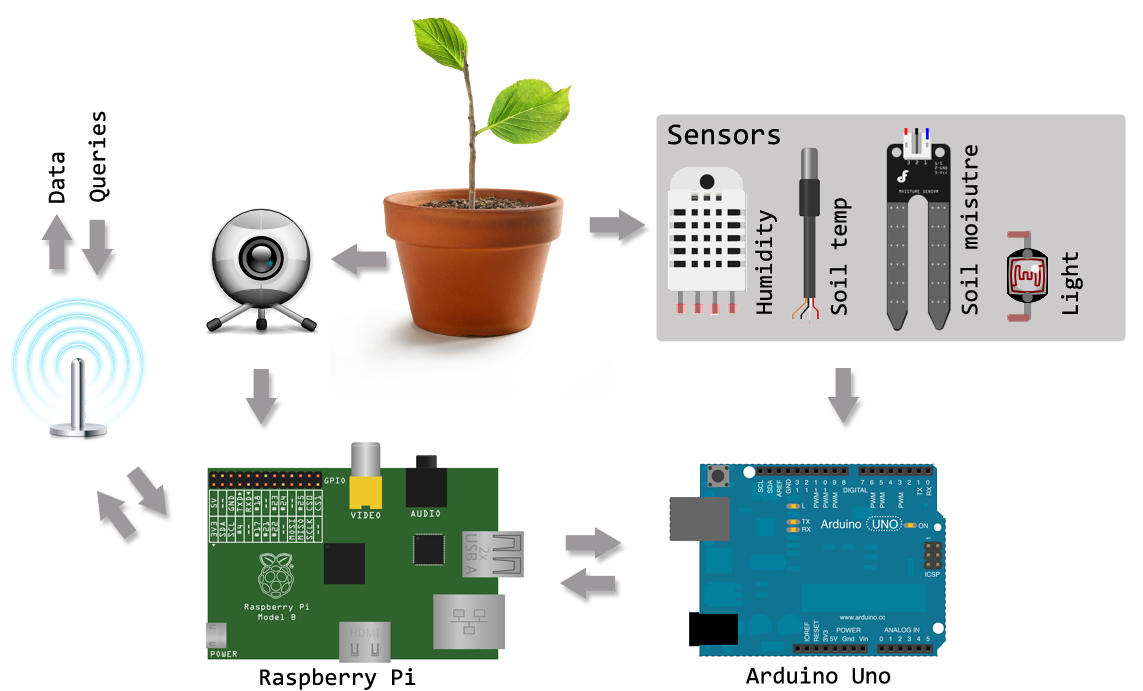
\includegraphics[width=1\textwidth]{img/hardware/application.png}
\caption{High-level illustration of the physical hardware components in Monoplant}
\label{fig:application}
\end{figure}

\section{Plant data collection}
At the lowest level in the information hierarchy is the hardware and software responsible for capturing and uploading environmental data regarding the plant. Like a patient in a hospital, the plant is connected to a range of sensors, each responsible for reading a specific variable that is important for the plant's functioning. These variables are sent to a computer, processed, and uploaded to the next level in the data hierarchy. In the following sections we will follow the data on its way from the plant's physical location to the "cloud" and the user.

\subsection{Sensors}

\def\arraystretch{1.8}
\begin{table}
	\begin{tabular}{@{}lp{250pt}@{}}\toprule
	Sensor               & Description \\ \midrule                                                                                                  
	TSL2561              & Digital luminosity sensor. Measures light in lux from 300-1100nm.                                            \\ 
	RHT03                & Digital humidity and temperature sensor. Measures relative humidity and temperature in Celsius.              \\ 
	DS18B20              & Digital waterproof temperature sensor. Measures temperature in Celsius.                                       \\ 
	DFRobot sku:sen0114  & Analog soil moisture sensor. Returns values between 0 and 900 depending on electrical conductivity of soil.  \\ \bottomrule
	\end{tabular}
	\caption{Sensors used in the application}
\end{table}


With the advent of the "internet of things", sensors are becoming available in many different forms and packages. They are cheap and can be used as modular building blocks in a wide range of applications, from automating tasks such as keeping a steady indoor-temperature, to measuring variables that humans cannot see. 

The sensors are able to capture information concerning the environment and transform it to data variables, which we can store and categorize. In total there are five different sensors connected to the plant, or in the plant’s vicinity: soil moisture, soil temperature, air temperature, humidity, and light intensity. 


%(write something about the sensortag)

The sensors we have used in this project are analogous to a volume controller on an amplifier. On an amplifier one can adjust the volume by varying the resistance in the signal going to the speakers. If we turn the volume up, the resistance goes down, and if we turn the volume down, the resistance goes up. Sensors work in the same way, but instead of controlling resistance with a volume knob, it is controlled by light, moisture or other environmental variables. 

To exemplify let's look at temperature sensors, or "thermistors". They vary their resistance in relation to the temperature. Since we already know how many volts we are sending to the thermistor on the one end, we can use the amount of volts we get back to calculate the resistance. In our application this is done by a voltage divider, which uses a formula as follows: 

\begin{equation}
V_{out}=\frac{R_{2}}{R_{1}+R_{2}}\cdot V_{in} 
\label{eq:vdiv1}
\end{equation}
Where $V_{out}$ is voltage out, $V_{in}$ is voltage in, $R_{1}$ is a given resistance, and $R_{2}$ is the resistance we want to calculate. For this example let's assume that $V_{in} = 5_{v}$, $V_{out} = 2_{v}$, and $R_{1} = 1K\Omega$. We solve this equation with regard to $R_{2}$
\begin{equation}
R_{2} = \frac{V_{out} \cdot R_{1}}{V_{in}-V_{out}}
\end{equation} 

\begin{equation}
R_{2} = \frac{2_{v} \cdot 1000\Omega}{5_{v}-2_{v}}
\end{equation} 

\begin{equation}
R_{2} = \frac{2000\Omega}{3}
\end{equation} 

\begin{equation}
R_{2} = 667\Omega
\end{equation} 

Then we can see that the calculated resistance is 667$\Omega$. This value can then be mapped to the correct unit of measure, in this case Celsius or Fahrenheit. 

As we are using digital sensors, all of these calculations are done internally in the sensors, and coded into a digital signal. This signal is then passed onto the next unit in our system, the Arduino.  

\subsection{Arduino}
%(Write about embedded systems. What other alternatives are there to the Arduino? )

Arduino is an open-source prototyping platform that makes it easy to interface low-level electronics (i.e., sensors) with higher-level electronics (i.e., computers). The core part of the Arduino is an Atmel\texttrademark Atmega microcontroller, which can be programmed by a computer over a USB port, using the Arduino programming language and the Arduino development environment \citep{Arduino}.

%We have used an Arduino Uno that has 13 digital input output pins (GPIO), five analog inputs, i2c inputs, and a USB port for serial communication. The soil temperature sensor and the temperature and humidity sensor are connected to the digital inputs through a 1K(ohm) pullup resistor. The pullup resistor is used to keep the voltage sent to the Arduino from fluctuating when the sensor is not sending any data. The TSL2561 luminosity sensor is connected to the A4/SDA and A5/SDL ports of the Arduino as it communicates over the i2c protocol. And the DFRobot soil moisture sensor is connected to A3 (Analog input 3) as it outputs analog voltage.  

\begin{figure}
\centering
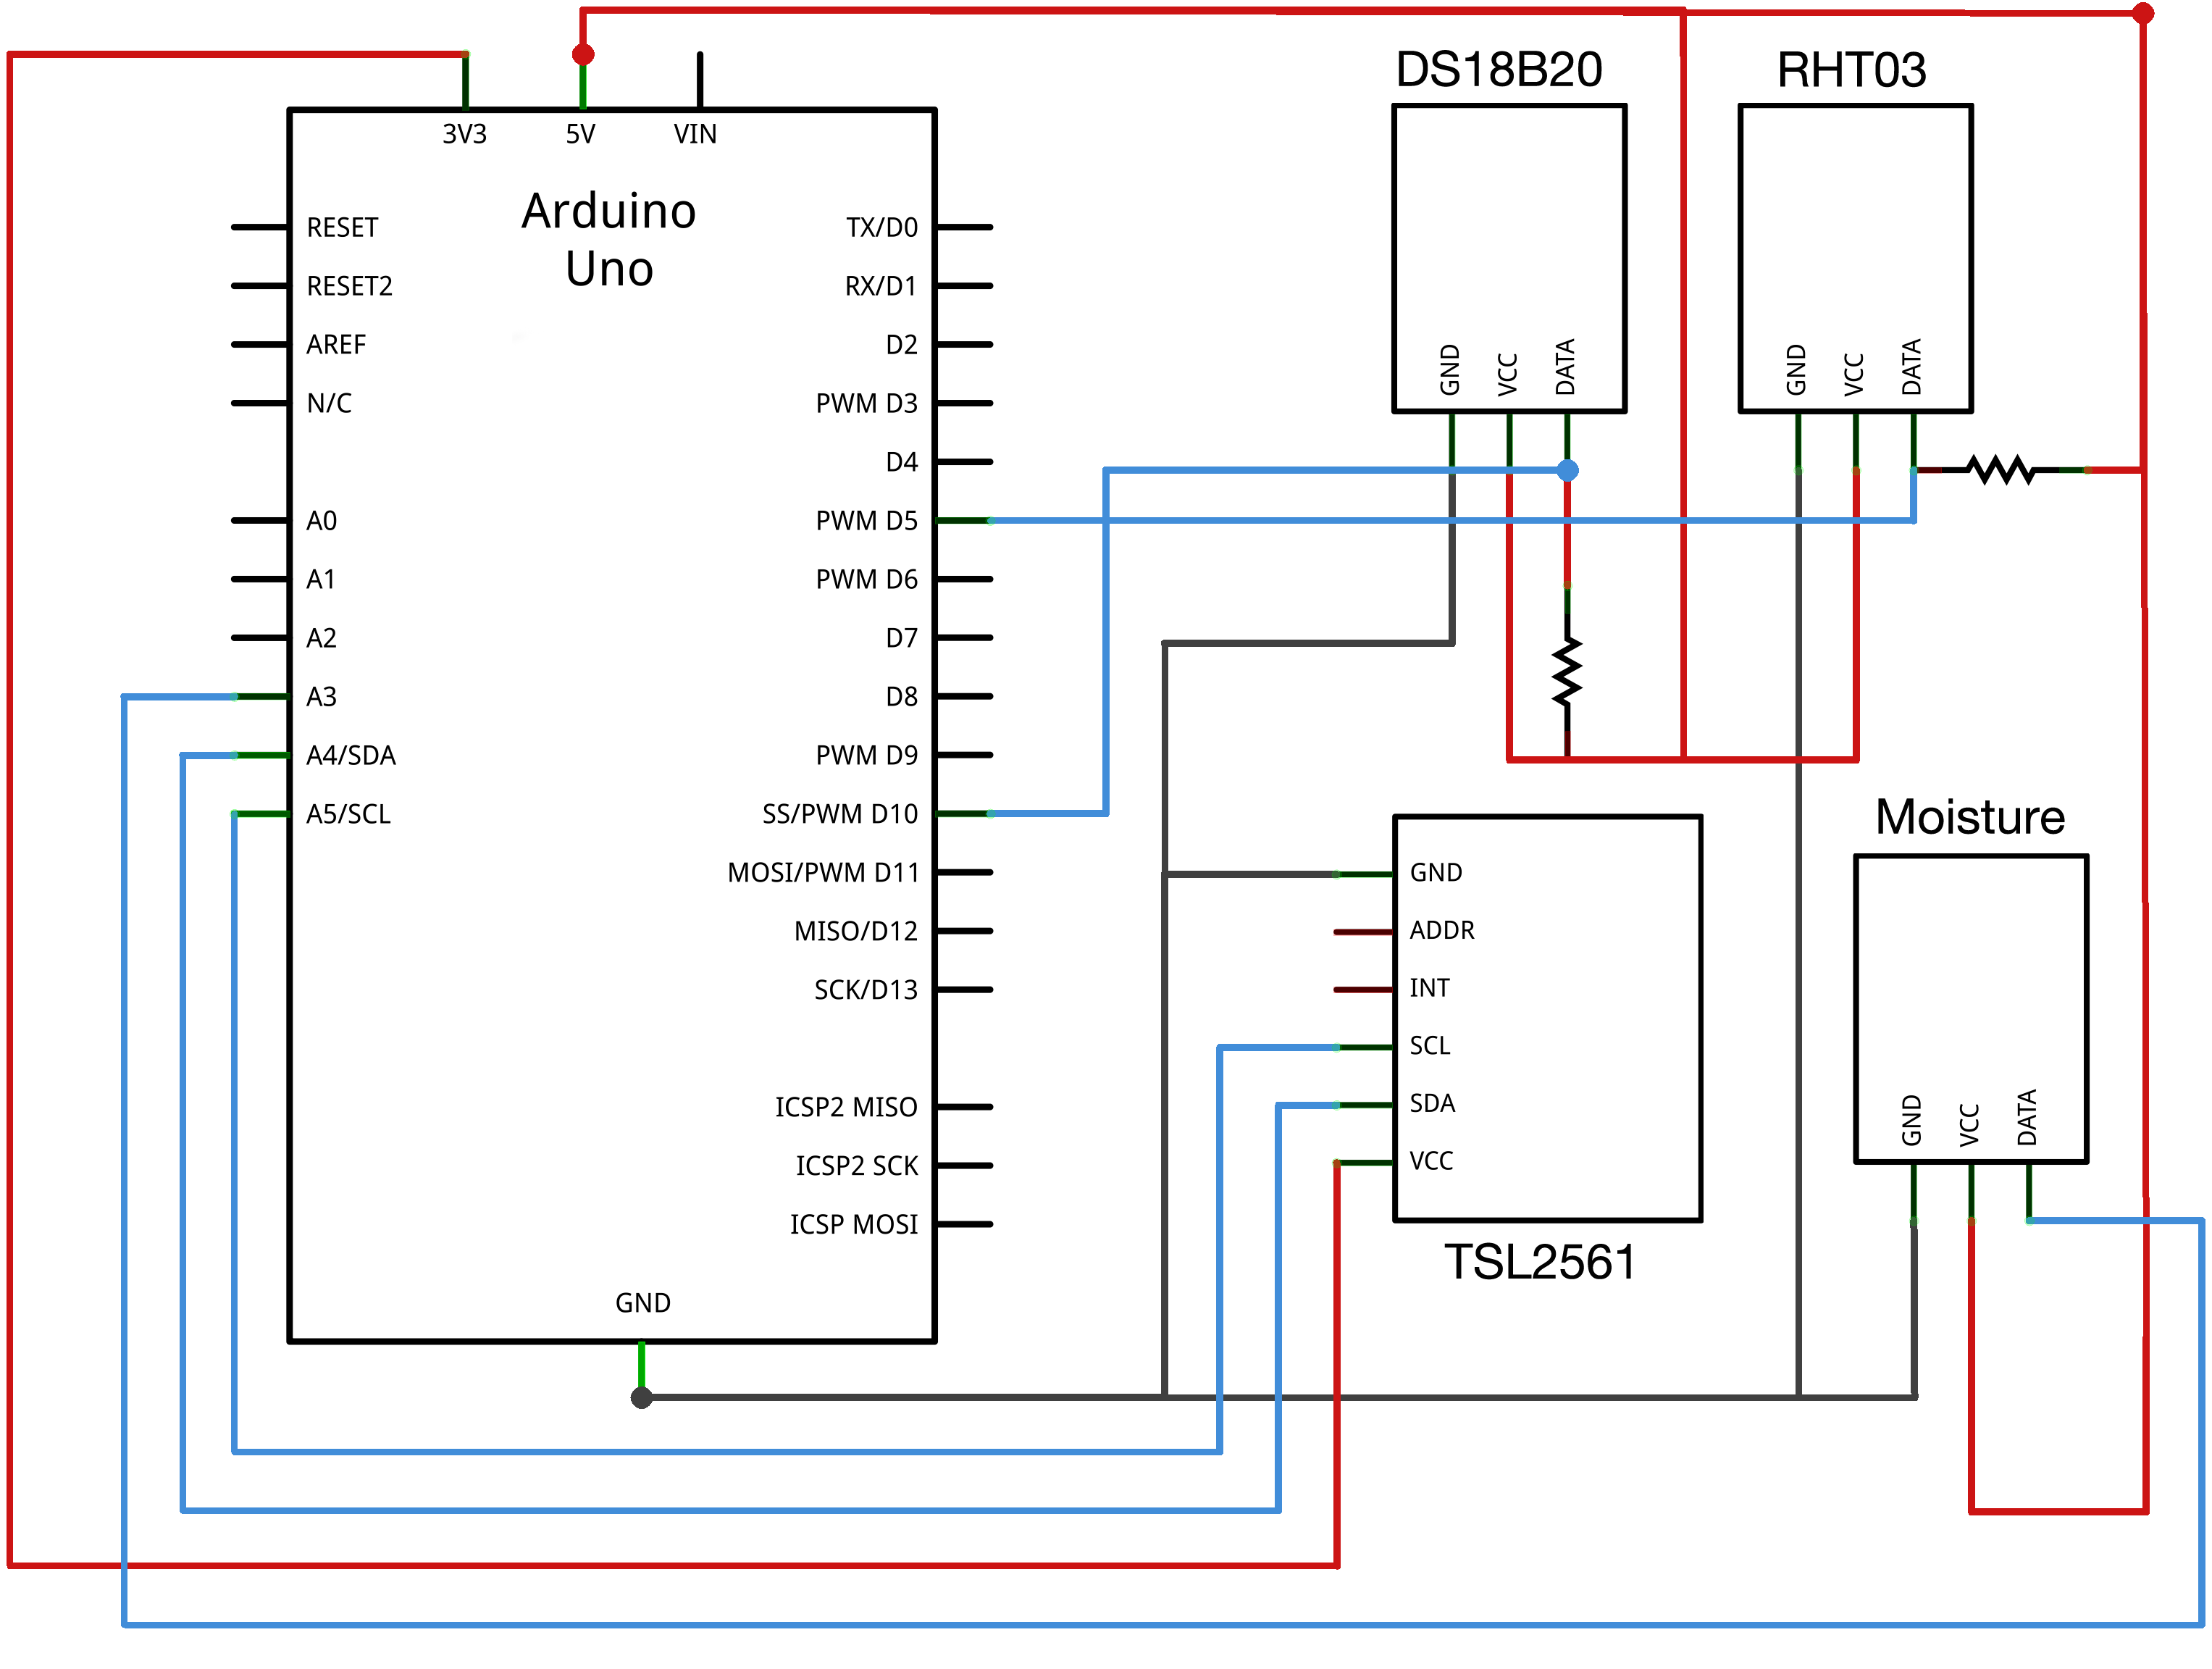
\includegraphics[width=1\textwidth]{img/hardware/Arduino_and_sensors_schem.png}
\caption{Schema diagram of Arduino sensor wiring. Pull-up resistors on the data line of the temperature sensors.} %The TSL2561 light sensor communicates over the i2c protocol (SDA,SCL), and the soil moisture sensor connects to analog input}
\label{fig:Arduino}
\end{figure}

The community surrounding Arduino is quite large, and we have therefore been able to find pre-written libraries for communicating with the different sensors. This has simplified the task of converting the digital signal to the correct units (Celsius, relative humidity, lux). 

In the case of the soil moisture sensor, it measures conductivity in the soil, and does not output moisture levels in any kind of universal measuring unit. But the conductivity measured in the soil is repeatable and proportional to the moisture level. Therefore we measured the resistance in air (high resistance), and in water (low resistance), and let these be the high and low points of a new unit called arbitrary moisture units (AMU) \citep{ch00ftech}.

The code residing in the Arduino runs a simple loop where it waits for a special character sent over serial communication through USB. If it receives this character it reads all the sensor values, and sends them back to the next device in the Monoplant system: the Raspberry Pi

\subsection{Raspberry Pi}
%(Why Raspberry? Beagleboard?)
The Raspberry Pi is a “cheap, accessible, programmable computer” \citep{Raspberrypi}, which is roughly the size of a credit card. Our model was released in early 2012 and contains two usb ports, audio and a SD-card slot. We have connected a wireless network adapter, a high-definition webcam, a powered USB-hub, and an Arduino to the Raspberry. The operating system running on it is a port of Debian Linux optimized for the Raspberry, called Raspbian. 

\begin{figure}
\centering
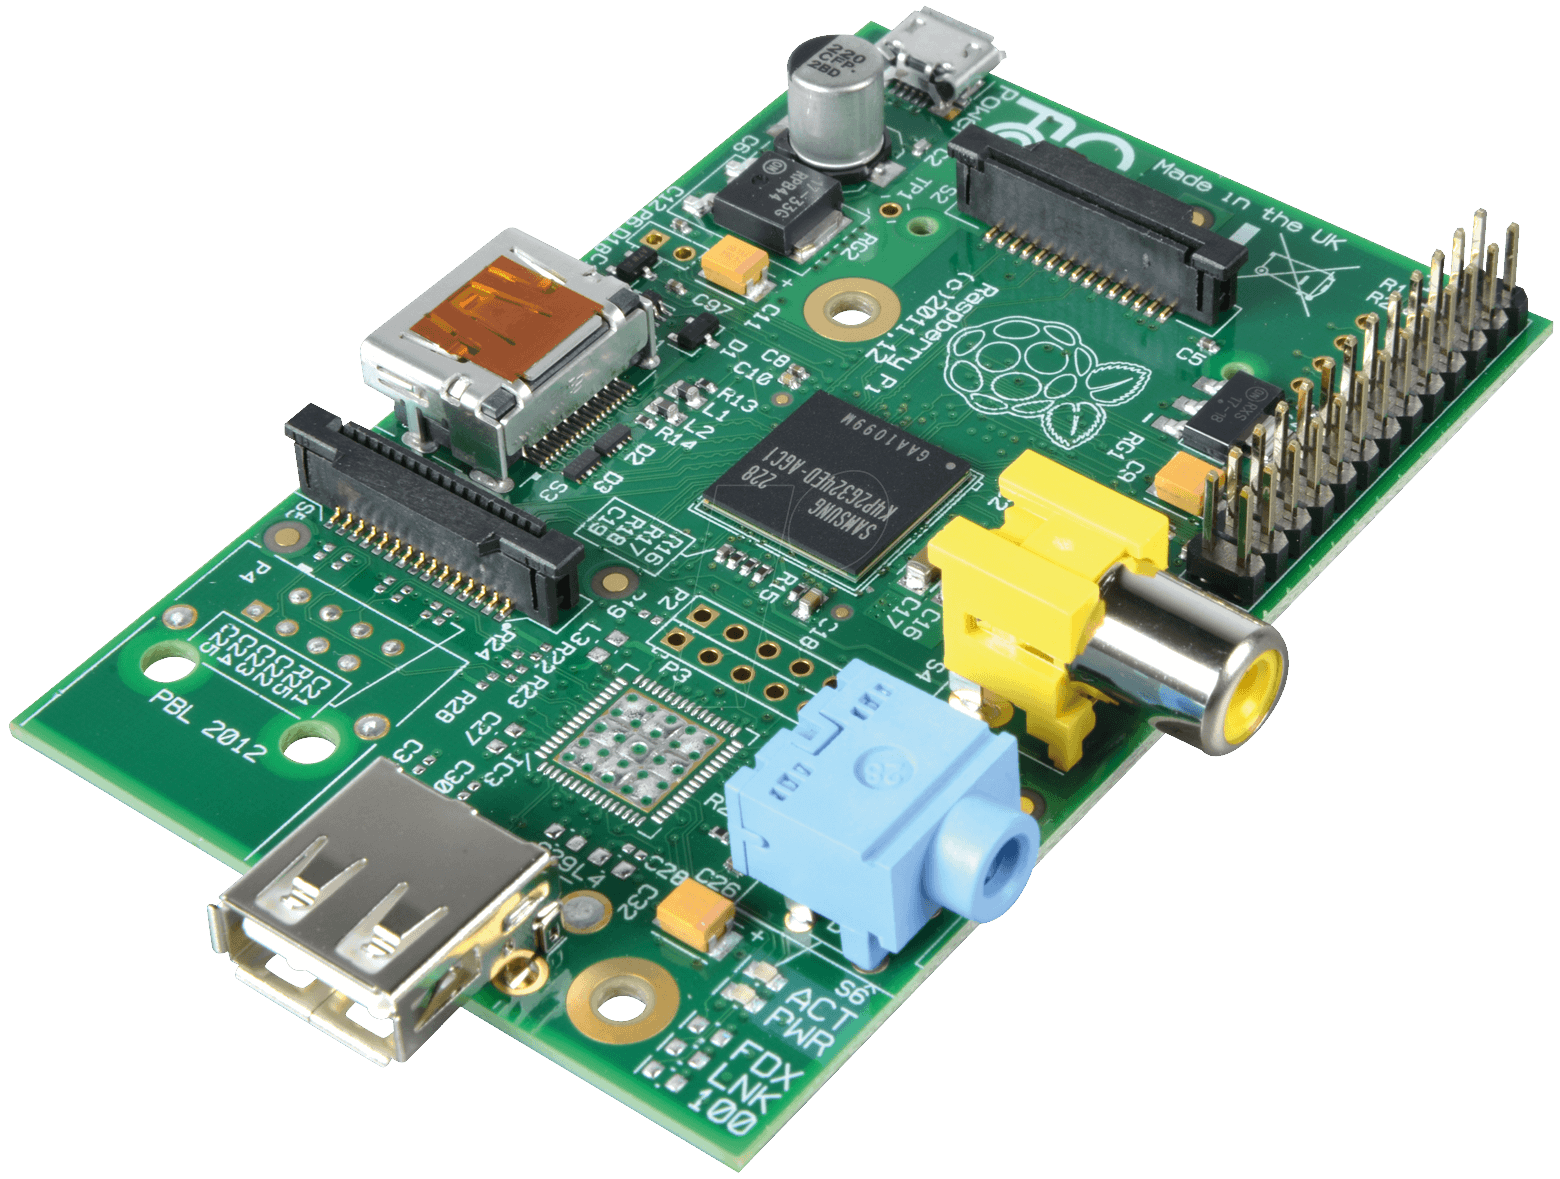
\includegraphics[width=1\textwidth]{img/hardware/raspberry.png}
\caption{Raspberry Pi}
\label{fig:Raspberry}
\end{figure}

%The GPIO-pins on the Raspberry works almost in the same fashion as the Arduino's digital input output pins. Thus we could in theory simplified the hardware by omitting the Arduino. The main reason for not doing this is that the Raspberry does not have an analog to digital converter (ADC). Therefore we would have to make a complex circuit involving an ADC to interface the Raspberry with the soil moisture sensor. In addition, we would most likely face timing issues. When we ask the digital sensors for data, they send the response immediately. If the unit receiving is not available to read the data, it gets lost. This can be a problem when using a high-level computer, as it performs multiple tasks in addition to reading sensordata. 

\subsubsection{Operation}
After booting up, a bash-script running an endless loop is called. The script snaps a photo of the plant using the webcam, and then runs a python-script responsible for collecting sensordata (see fig.~\ref{fig:Raspberrycode}). Since we sometimes can get erroneous values from the sensors, we read 15 values and upload the median value. These values, along with the photo captured by the webcam, are then passed on to the next logical unit in the Monoplant system. 

%http://en.wikibooks.org/wiki/LaTeX/Packages/Listings
\begin{figure}
	\begin{lstlisting}[style=htmlcssjs]
//instantiate lists
airtemp = []
humidity = []
light = []
soiltemp = [] 

for x in xrange(1,15): 
	ser.write("r") //Ask Arduino for data
	variables = ser.readline() //Read the data
	sensorReadings = variables.split('|') 
		//Split string on |

	airtemp.append(float(sensorReadings[0]))
	humidity.append(float(sensorReadings[1]))
	light.append(float(sensorReadings[2]))
	soiltemp.append(float((sensorReadings[3])[:-2])) 

//calculate and post the median using numpy
postData(np.median(airtemp),np.median(humidity),np.median(light),np.median(soiltemp)) 
	\end{lstlisting}
\caption{Reading sensor values from Arduino on Raspberry Pi, written in Python}
\label{fig:Raspberrycode}
\end{figure}

\section{Data processing and database}
When the data has been gathered at the low level hierarchy, it is stored in the cloud. This is done by posting the data to an application programming interface (API) on our web server. The main function of an API is to be a means of communication between different software, in our case the data collector, and the user interface. After some research on web-API design, we decided that a REST architectural style was best suited for our application. 
%REST uses URIs and HTTP by default, the data you send is the data you send. This meas that the data is easy to use out of the box, 
%SOAP can use URIs and HTTP, the data you send becomes larger as verbose SOAP-standards are added to the data.

\subsection{Representational State Transfer (REST)}
REST is an architectural style for distributed hypermedia systems \citep{fielding2000architectural}. In Fielding's dissertation, he writes about the interaction constraints of REST that is introduced in order to limit how a distributed system can be constructed. 

\begin{enumerate}
\item{} \emph{Client/Server} - This constraint separates the concerns of the client and the server. By separating these concerns, one secures that the two can evolve independent of each other. The client does not care about the internal logic of the server, and the server does not care what the client does with the data. This gives us the ability to separate the concerns of data collection, data storage and data visualization, which gives us the freedom to change the internal logic of any one of these without worrying about breaking the other two. It also means that we can create several different clients either for collecting data or displaying data.

\item{} \emph{Stateless} - The communication between client and server must be stateless. The request from client to server must contain all the information needed to understand the request. In practice this gives the client the responsibility to keep track of the state.

\item{} \emph{Caching} - In order to reduce the number of requests and improve efficiency, the server can state which responses the client can reuse when sending equivalent requests. This can greatly enhance user-perceived performance, but at the same time reduce reliability if cached data differs from what would have been delivered by the server on a request. We could theoretically cache almost everything since our data belongs to specific timestamps, and the chances that a sensor value is updated at a later time are minimal. However, since we are developing a prototype and have the need for rapid changes in the implementation, we have experienced that the need for reliable data exceeds the need for fast performance.

\item{} \emph{Uniform interface} - This is a rather complex constraint in terms of RESTful API design, and is the reason for a lot of discussions around implementation of true REST. Fielding describes a REST interface to be:

\begin{quote} ...efficient for large-grain hypermedia data transfer, optimizing for the common case of the Web, but resulting in an interface that is not optimal for other forms of architectural interaction. \citep[p. 82]{fielding2000architectural} 
\end{quote}

In an applied context this means that the server has resources that can be referenced via URLs and operated through the HTTP-verbs. In order to be a true REST interface, an API can have any resource available through URLs, but the only methods in which one can operate the resource is POST, GET, PUT and DELETE.

\item{} \emph{Layered system} - This constraint tells us that a REST interface may hide complexity hierarchically, by masking information so each component cannot "see" beyond the immediate layer with which they are interacting. \citep{fielding2000architectural}

\item{} \emph{Code on demand} - An optional constraint, allowing the server to serve executable code to the client. 

\end{enumerate}

REST is an architectural style, not a strict standard. It allows for flexibility, but at the same time promotes best practice. The goal for our API was to provide a way of storing and accessing plant data in the cloud, first and foremost for our own client side applications. Our objective was to create something that worked for us. A pragmatic approach to REST gave us the flexibility to create an API that gets the job done. In the following chapter we will describe how our API works, and discuss some choices we made in the implementation process.

\subsection{Application Programming Interface}
Our first implementation of the API was written in PHP using the framework Codeigniter. This worked well for a while, but after having made several dirty hacks and workarounds we decided to look for other options. After researching Ruby on Rails and their focus on "convention over configuration", we found that it was a framework well suited for building our API.  

\begin{quote}
Ruby on Rails is an open-source web framework that's optimized for programmer happiness and sustainable productivity. It lets you write beautiful code by favoring convention over configuration \citep{rubyonrails.org}. 
\end{quote}

Ruby on Rails (RoR) makes the assumption that there is a "best" way of doing things, and encourages that way. It emphasizes well-known software engineering principles such as convention over configuration, don't repeat yourself (DRY), model-view-controller and REST.

Our web server is running on Amazon Elastic Compute Cloud (ec2), a virtual computer service with low costs and extensive configuration options. We chose this because we needed to be able to configure the server for our purposes and install several libraries and applications onto the server. 
%We wanted to create the API The API is created with Ruby on Rails to 

Our API is a server-side Web-API that can be accessed through the HTTP-protocol. To use it, one can send a request to the domain of the API from any client that can send HTTP-requests. The API will interpret the request and respond based on how the interpretation went. Since our API is based on the REST architectural style, it adheres to how the HTTP-protocol is built, meaning that a resource has a unique identifier, a URI, and some uniform actions called the HTTP-verbs which the resource can be operated with. There are 8 methods in the HTTP/1.1 protocol \citep[p. 36]{fielding1999hypertext}, but only four of them are of interest when speaking of resources. These are the four basic functions of persistent storage in computer programming, often referred to as CRUD (Create, Read, Update and Delete), but in HTTP their names are POST, GET, PUT and DELETE. 

The Monoplant API has three resources: Plants, Sensorvalues and Videos. To create a plant, one can send a POST request to the URL: \begin{verbatim}http://Monoplant.me/plants.json\end{verbatim} A post request also needs information about the plant to create, in this case we will pass that information in the json-format (see fig.~\ref{fig:postdata}).

\begin{figure}
	\begin{lstlisting}[style=htmlcssjs]
{
	"plant": {
		"name": "Alfa",
		"location": "Intermedia",
		"plant_type": "Alfalfaspire"
	}
}
	\end{lstlisting}
	\caption{POST plant json data}
	\label{fig:postdata}
\end{figure}

For the API to know how to interpret this information in json, we also need to pass a parameter in the header called Content-type, this variable will be set to “application/json”. When we pass this request, the API will create a plant with the information we gave it, and give a HTTP response with the code: \verb@"201 created"@. The response contains a header and a body. The header has some meta-data about the request and the body will contain a representation of the created plant (see fig.~\ref{fig:plantresponse}).

\begin{figure}
	\begin{lstlisting}[style=htmlcssjs]
{
	created_at: "2013-09-17T10:45:17+02:00"
	id: 1
	location: "Intermedia"
	name: "Alfa"
	plant_type: "Alfalfaspire"
	updated_at: "2013-09-17T10:45:17+02:00"
}
	\end{lstlisting}
	\caption{Plant response in json}
	\label{fig:plantresponse}
\end{figure}

If we look at this representation, we see that the API has added an ID to the plant as well as the two data attributes \verb@created_at@ and \verb@updated_at@. Since we now have the id of the plant, we can tell the Raspberry Pi to start adding sensor values for that specific plant. The Raspberry will create a request using the data it gets from the Arduino and the image from the webcam and finally send that POST request to the URL:\begin{verbatim}http://Monoplant.me/plants/1/sensorvalues.json \end{verbatim}

As in the first example the API will interpret the request, store the data, and respond with a status code: \verb@"201 created"@. In the background, the API will generate a thumbnail of the image and upload both the thumbnail and the original to another static server, finally storing the URL for both of them in a database. The response body ends up looking as shown in figure~\ref{fig:sensorvaluesresponse}. If we need to look at this sensorvalue at a later time, we can simply do a GET request using the sensorvalue id we got from the previous response and call the URL:\begin{verbatim}http://Monoplant.me/plants/1/sensorvalues/10037.json \end{verbatim} This will make the API respond with a status code \verb@"302 Found"@, and the body will look just like the previous response body, unless it has been updated in the meantime. Note that the URL is built up according to which resource we are trying to operate. See table~\ref{fig:RESTurl} for an overview of how these URLs are built up.

Now that the data from the plant is securely stored in a database and accessible through the API, we move on to how these data are further processed to generate time-lapse videos. 

\begin{figure}
	\begin{lstlisting}[style=htmlcssjs]
{
	airTemp: 22.14
	created_at: "2013-09-17T10:49:43+02:00"
	humidity: 38.5
	id: 10037
	img_url: "http://s3-eu-west-1.amazonaws.com/plantespann/2013/9/17/original/10037.jpg?1379407782"
	light: 1702.5
	photo_content_type: "image/jpeg"
	photo_file_name: "viewcam.jpg"
	photo_file_size: 204358
	photo_updated_at: "2013-09-17T10:49:42+02:00"
	plant_id: 1
	soilMoisture: 54
	soilTemp: 22.25
	thumb_url: "http://s3-eu-west-1.amazonaws.com/plantespann/2013/9/17/thumb/10037.jpg?1379407782"
	updated_at: "2013-09-17T10:49:43+02:00"
}
	\end{lstlisting}
	\caption{Sensorvalues response from Monoplant}
	\label{fig:sensorvaluesresponse}
\end{figure}



\bgroup
\def\arraystretch{1.8}	%  margin for cells 1 is default
\begin{table*}
	\centering
	\begin{tabular}{@{}lp{250pt}@{}} \toprule
		\textbf{part of URL}&	\textbf{meaning}\\ \midrule
		\texttt{http://}&	the protocol we access the API through\\ 
		\texttt{Monoplant.me}&	the domain of the API\\ 
		\texttt{/plants/(:id)}&	\texttt{/plants} states that we want to access a resource named plant \\ &
		\texttt{/(:id)} is a number representing the specific plant we want to access\\ 
		\texttt{/sensorvalues/(:sid)}&	\texttt{/sensorvalues} states that we want to access a resource named sensorvalue. Since this comes after \texttt{/plants/(:id)} it means that we will get sensorvalues owned by the plant with \texttt{(:id)}. \\ &
		\texttt{/(:sid)} is a number representing the specific sensorvalue we want to access\\ 
		\texttt{(.format)}&	 \texttt{.format} can be blank, .html, .xml or .json. If it is blank, the API will respond with the default format, in our case html. \\ \bottomrule
	\end{tabular}
	\caption{How a REST-url is built up}
	\label{fig:RESTurl}
\end{table*}
\egroup

\subsection{Generating time-lapse videos}
Regular video cameras capture 24 to 30 images or frames per second (fps), and play them back at the same rate. The events in the video will then unfold at the same speed in which they happened during the shoot. Time-lapse photography utilizes this principle by slowing down the rate at which images are captured, while maintaining the playback rate. So for instance if we captured one image per second, and played it back at 24 fps, one second in the film would equal 24 seconds in real life. Thus when played back, time would appear to move faster. This makes it possible to pronounce changes that are subtle to the human eye such as: a sunset, moving clouds, or a plant growing.  

Each day at midnight the system collects all the images taken during the day, and combine them to a time-lapse video played back at 30 frames per second. As the Raspberry Pi captures approximately one picture per minute, one second in the video equals 30 minutes in real life. One picture each minute equals \begin{math} 60min*24hours=1440 \end{math}
pictures each day, which, if we divide it by 30 frames per second gives us a 48 second video representing 24 hours in real life. This equals a speed increase of 1800 times. 

%Logically, to adhere to the principle of separation between data generation, storage and presentation. The Raspberry would generate the timelapse videos itself, and then push them to the API. But in an effort to reduce the amount of load on the Raspberry Pi, we decided to compile the timelapse videos needed on the same server as the API. By doing so the amount of data transferred from the PI to the API is also reduced, as the API server already has the processing power and the images needed for the generation. 

\subsubsection{HTML5 Video Element}
Prior to HTML5 there was no standard way of implementing videos on web pages. Therefore the web was filled with a myriad of different solutions, with QuickTime, RealPlayer, and Flash being the most prominent \citep{pilgrim2010html5}.

In HTML5 we have a new standard \verb@<video>@ element that in theory should give us support for native video in all browsers. But due to the nature of video-files, problems arise when users have different operating systems and different browsers. 

A video file consists of a container, a video codec, and an audio codec. The container defines how the content within is stored, the video codec defines how the video stream is encoded, and the audio codec defines how the audio is encoded. Since there exists numerous containers, video- and audio codecs, endless permutations are possible. Therefore it is not likely that we will have a combination that would work in all browsers in any foreseeable future \citep{pilgrim2010html5}.

In order to maximize compatibility in our application, we decided to encode video in three different formats: H.264+MP4, Webm and Theora (see table~\ref{tab:videosupport}). This is done via a bash script that runs every night. First, we run a Perl script for "deflickering", i.e., calculate and convert the images to a median brightness to reduce video flickering. Then we use the programs Mencoder and FFmpeg2theora to create H.264, webm and theora videos. And finally, the videos are posted to the respective plants in a database, using the API. 

Thus, after 24 hours of collecting and storing data, videos in different formats are generated and Monoplant is ready to display information to the users, which takes us to next logical unit in the system.
%After the data has been collected from the sensors and uploaded through the API. And we have generated timelapse videos in different formats. We are ready for the next logical unit in the Monoplant application, displaying information to the users. 

\begin{table*}\centering
\begin{tabular}{@{}lcccc@{}} \toprule
Codecs/containers & IE & Firefox & Safari & Chrome \\ \midrule
Theora+Vorbis+Ogg & ~                 & 3.5+    & ~      & 5.0+   \\ 
H.264+AAC+MP4     & 9.0+              & ~       & 3.0+   & 5.0+   \\ 
WebM              & 9.0+              & 4.0+    & ~      & 6.0+   \\ \bottomrule
\end{tabular}
\caption{Video support in different browsers \citep{pilgrim2010html5}}
\label{tab:videosupport}
\end{table*}

%http://en.wikibooks.org/wiki/LaTeX/Packages/Listings
% \lstset{language=bash} 
% \begin{figure}
% \begin{lstlisting}
% #!/bin/bash
% #get yesterdays date
% year=`/bin/date -d '1 day ago' +%Y`

% date=`/bin/date -d '1 day ago' +%m`
% month=`expr $date + 0`

% date=`/bin/date -d '1 day ago' +%d`
% day=`expr $date + 0`

% #copy files
% cp /mnt/s3/plant_2/$year/$month/$day/original/* /home/ubuntu/bin/timelapse/source_folder_of_pictures/

% #run deflicker
% perl /home/ubuntu/bin/timelapse/timelapse-deflicker.pl

% #step into deflickered folder
% cd /home/ubuntu/bin/timelapse/source_folder_of_pictures/Deflickered

% #get a file for the coverpicture
% ls | grep -v files.txt > files.txt 
% coverpicture=$(sed -n '100p' < files.txt)
% rm files.txt

% #create video h264
% /usr/bin/mencoder -idx -nosound -noskip -of avi -ovc x264 -x264encopts pass=1:bitrate=2000:crf=24:bframes=0 -o output.avi -mf fps=30 'mf://@files.txt'
% /usr/bin/MP4Box -aviraw video output.avi
% /usr/bin/MP4Box -add output_video.h264 output.mp4

% #create video theora (ogv)
% /usr/local/bin/ffmpeg2theora --noaudio -v 7 output.avi

% #create video webm
% /usr/bin/mencoder -idx -ovc lavc -nosound -of lavf -lavfopts format=webm -lavcopts threads=4:vcodec=libvpx -ffourcc VP80 output.mp4 -o output.webm

% \end{lstlisting}
% \caption{Video encoding for HTML5}
% \label{fig:videoencoding}
% \end{figure}

\section{User interface}
The user interface (UI) of Monoplant is where we visualize the data from the API to the users. It is accessible through web (\url{http://www.monoplant.me}), and displays correctly on most devices due to a responsive design. The UI is built with RoR as the web application framework, Bootstrap as the design framework, and Highcharts as the graph framework.   

The main web page of each plant represents the current state of the plant. On the left side, it displays the last picture with the corresponding temperature, humidity, light and soil moisture. On the right side, there is a timelapse video from the day before, with a corresponding graph displaying all the sensorvalues throughout that day (see fig.~\ref{fig:mainpage} on page~\pageref{fig:mainpage}). 

On the top of the page there are two menu items. The first  is called \emph{videos} and links to the video overview. This is a page containing all the videos for the plant selected. In relation to each video, the max and min values for all the different sensors during that day is shown. The second menu item is called \emph{graphs} and is a drop-down menu with links to graphs for each of the different sensors. In addition there is a link to the graph containing all the sensorvalues for the last 24 hours. 

During our work with the UI, there were two aspects that proved to be particularly challenging: relative graphs, and connecting the timelapse videos to the graph. In the following sections the work to overcome these obstacles will be explained. 

\begin{figure}
\centering
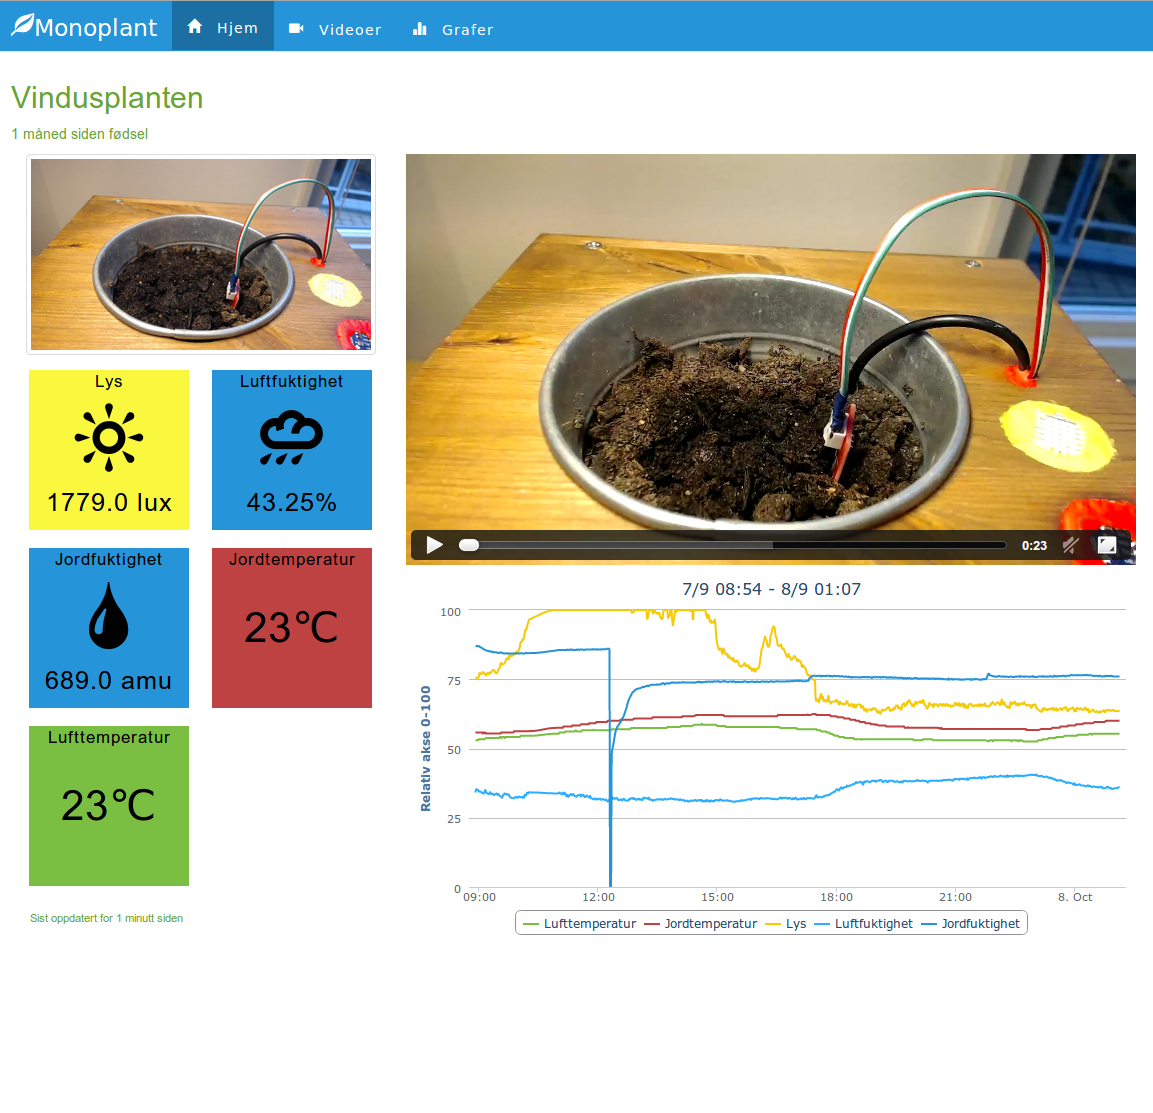
\includegraphics[width=1\textwidth]{img/interface/mainpage.png}
\caption{Screenshot from user interface}
\label{fig:mainpage}
\end{figure}

\subsection{Highcharts}
There are a few serious JavaScript chart libraries available with various types of focus, flexibility and documentation. We ran some tests with Google charts, d3.js and Highcharts, and found that Highcharts provided the most extensive documentation as well as an easy to understand interface. 

The first graph we had to make was a graph containing all the plant data from a given time corresponding to a timelapse video. This meant putting temperature, light, humidity and soil moisture in the same graph, even though they all have different units. 



\begin{figure}
\centering
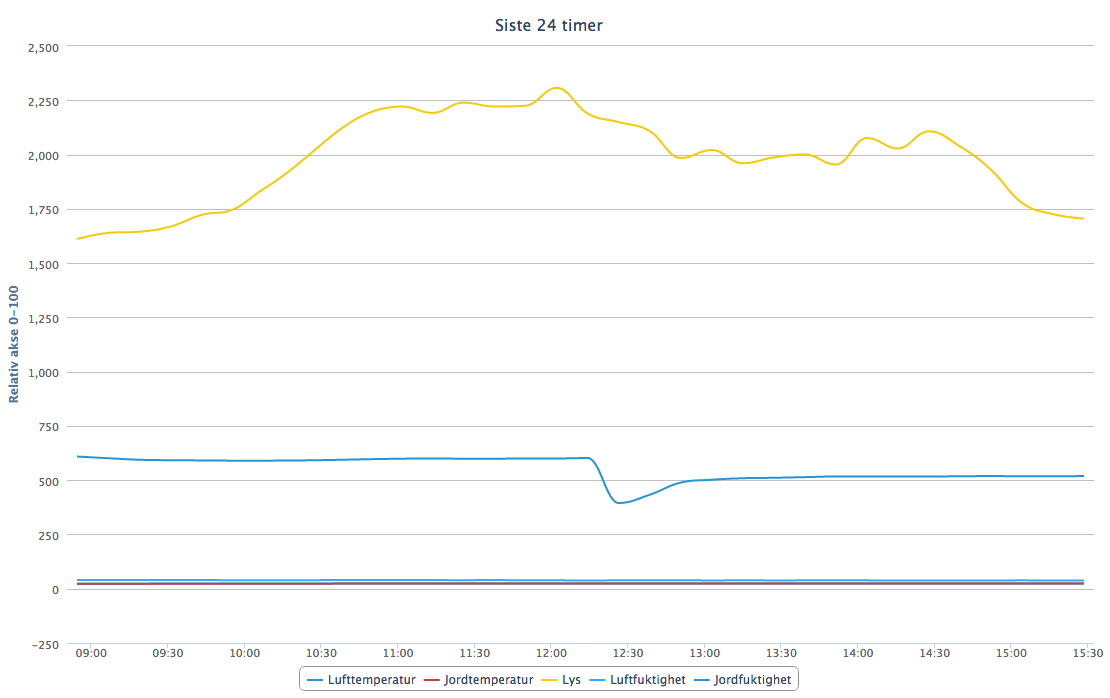
\includegraphics[width=1\textwidth]{img/interface/badgraph.png}
\caption{Screenshot from an unsuccessful graph}
\label{fig:badgraph}
\end{figure}

Our first attempt was done without manipulating the data at all. As Highcharts scales the y-axis based on the element with the highest values, the element with small values appeared as straight lines at the bottom of the graph. In figure~\ref{fig:badgraph} we tried to combine light levels of 2000 lux with temperature levels at $22\,^{\circ}\mathrm{C}$, and as we can see, all the elements except light and humidity are concentrated at the bottom. 

For this graph to display the environmental changes during a day we needed to create a relative scale and map the values to that scale. To exemplify, lets say you have a number \ensuremath{X}, which has a value between \ensuremath{A} and \ensuremath{B}, and you want to map it to a value \ensuremath{Y}, between \ensuremath{C} and \ensuremath{D}. The function is similar to calculating percentage and can then be written as: 
\begin{equation}
Y = \frac{(X-A)}{(B-A)} * (D-C) + C
\end{equation}

%This becomes a slightly more advanced version of calculating percentage (see figure~\ref{fig:mapfunc} on page~\pageref{fig:mapfunc}).

%We chose an output scale from 0 to 100 and wrote a function according to figure~\ref{fig:mapfunc} that mapped the values based on what type of data it was. We set the input scales as can be seen in figure~\ref{fig:mapscale}.

\begin{figure}
	\begin{lstlisting}[style=htmlcssjs]
{
	humidity: { min: 10, max:100 },
	soil temperature: { min:15, max:30 },
	light: { min: 400, max:2500 },
	air temprature: { min: 15, max: 30 },
	soil Moisture: { min: 0, max: 700 }
}
	\end{lstlisting}
	\caption{Mapping scales}
	\label{fig:mapscale}
\end{figure}

Through trial and error, we chose the \ensuremath{C} and \ensuremath{D} values of each unit (see fig.~\ref{fig:mapscale}). Then, after running the data through our new function all the units became visible (see fig.~\ref{fig:goodgraph} on page~\pageref{fig:goodgraph}). As we have mapped all the units to relative units, information of the values at the specific data points is lost. But as the graph is displayed along with the video, we wanted to keep the information level low.  

\begin{figure}
\centering
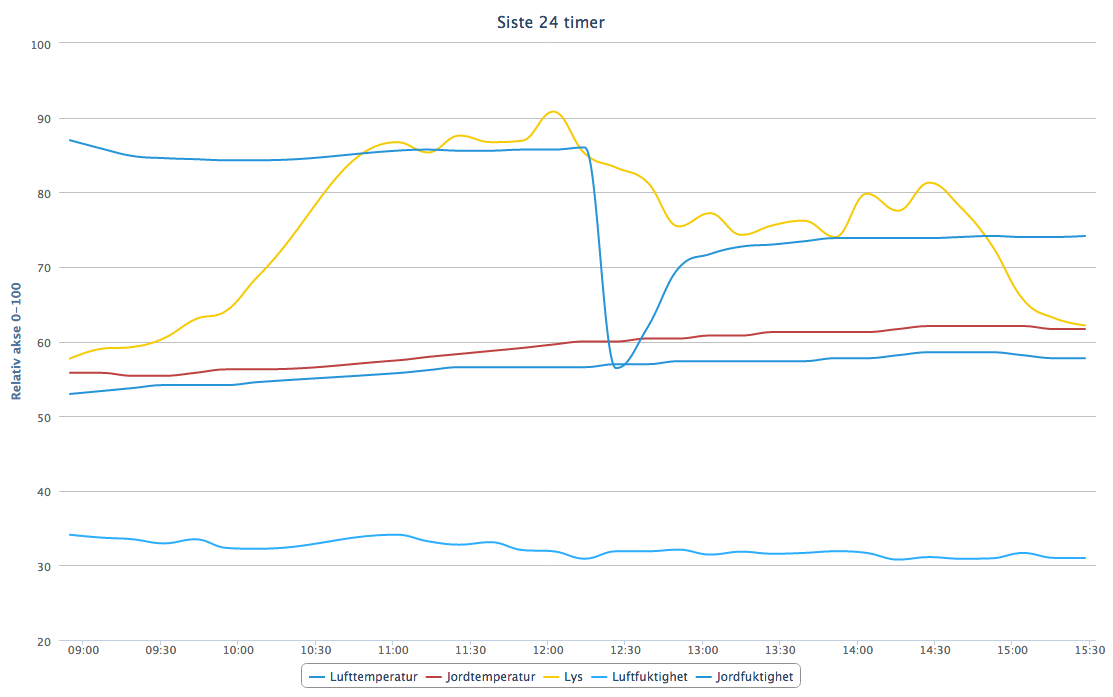
\includegraphics[width=1\textwidth]{img/interface/goodgraph.png}
\caption{Screenshot from a successful graph}
\label{fig:goodgraph}
\end{figure}

%To make sure one can read the appropriate sensorvalues we provide several other graphs, one for the last 24 hours, very similar to the video graph. The only difference is that we have included a mouse-over interaction technique with a tool-tip that displays the actual values alongside the corresponding image of the plant \citep[p.254]{kluge2010simulation}.

Apart from the video-graph and the last 24 hour-graph we provide singular line graphs for each variable. This gives us the ability to display graphs with correct y-axes. 
%The user can select time period for these graphs by interacting with the small graph on the bottom. 

\subsection{Connecting video and graph}
%explain objective
In order to present how changes in sensor variables manifested themselves physically in the plant, we wanted to connect the graph and the timelapse video. The visual solution became to present the video above the graph, both contained within the screen. As the video is playing, a vertical line layered above the graph moves from left to right representing the current point in the video. 

The HTML5 video-element can be accessed through JavaScript, and by checking the state of the video we are able to make the Highcharts graph follow the video based on the \verb@currentTime@ of the videoelement.

\begin{figure}
	\begin{lstlisting}[style=htmlcssjs]
function startVideo(){
	 interval = setInterval(function() {
		 var curtime = video.currentTime.toFixed(2);
		 if(curtime!= lastcurtime){
	 lastcurtime = curtime;
	 curmarker = Math.round(curtime*30);
	 stepTooltip(curmarker);
		 }
	 }, 33);
}

function stopVideo(){
	clearInterval(interval);
}
	\end{lstlisting}
	\caption{Video and graph connection code, written in JavaScript}
	\label{fig:videocode}
\end{figure}

By binding \verb@startVideo()@ to the play-event of the video-element and \verb@stopVideo()@ to the pause and stop event, we are able to move the graph marker as the video plays. The video-element has a built-in event called \verb@timeupdate@, which is triggered when the video's time is changed. However, in practice this event only appeared 3-7 times per second, giving a lagging experience of the graph marker. To overcome this we made a custom function using \verb@setInterval@, which turned out to be a lot faster and more reliable, providing a smooth flow of the graph marker. 


%The reason for using \emph{setInterval} instead of the videos built-in event \emph{timeupdate} is that it is not specified how often the event will fire, but by testing we found that it was somewhere between 3-7 times per second, varying randomly from second to second. This was not often enough as the video had a framerate of 30 frames per second, which meant updating the graph at 1/10 of the speed of the video, resulting in a laggish experience of the graph. We experienced that using \emph{setInterval} gave use much more accuracy when setting it to run every 33th millisecond. No browsers guarantee that the performance of \emph{setInterval} will be faster than 50 ms, but by running tests \citep{adequatleyqood}, we found that the Chrome browser ran this on an average of 4.5 ms. Even though this can be slower when considering the load on the browser when playing a video, we found that in practice most browsers were able to play the video and update the graph simultaneously. 

 %!TEX root = ../document.tex
\chapter{Theoretical perspective \& concepts for analysis}

In this chapter we will lay forth the theoretical perspective and theoretical concepts we will apply in this thesis. First we will introduce the \emph{sociocultural perspective} and highlight some key points including \emph{institutional practices}, \emph{zone of proximal development} and \emph{scaffolding}. Further we will look at \emph{multiple external representations} and lastly the concept and method of \emph{Inquiry learning}.

\section{Sociocultural perspective}

%The sociocultural perspective may be thought of as the synthesis of the behavioristic thesis and cognitive antithesis. The behavioristic model focuses on the role of the individual and the notion that knowledge arises through individual drill and practice. In contrast, the cognitive model focuses on the environment and the notion that the environment provides raw material for testing innately conceived hypotheses, thus focusing on instruction methods and acquisitional models. The sociocultural perspective considers the individual in the context of their environment, with a focus on means of mediation between the two. Thus, action is the primary unit in sociocultural analysis, which will be elaborated further in the following paragraphs. 

%The sociocultural perspective considers the individual in the context of their environment, with a focus on means of mediation between the two. Thus, action is the primary unit in sociocultural analysis, which will be elaborated further in the following paragraphs. 


In a biological sense the human species has not evolved significantly the last ten thousand years or so. In fact, changes in our gene pool are only minor, and can’t explain the difference between modern people and people of the Stone Age. Still we are able to achieve tasks that would have been impossible for our ancestors \citep{saljo2001laering}.

The explanation of this discrepancy from a sociocultural perspective becomes evident when one takes into account the \emph{tools} and \emph{signs} we use to mediate the world. We have created a culture where each of the \emph{tools} and \emph{signs} we use has a long history embedded in them. For instance if you are given the multiplication problem 122\texttimes284, you can flip up a calculator and get the answer instantaneously. Similarly, if you were to solve the multiplication problem 7\texttimes4 you can look up in a multiplication table and find the answer easily. These \emph{cultural tools} (calculator and multiplication table) enable you to make sense of the world in a different way than our ancestors. 

From the example given above we can see that there is an “irreducible tension” between the agent and the cultural tool \citep{wertsch1998mind}. Without the multiplication table you would not be able to solve the problem. But the multiplication table is not enough, as it would have been useless without a skilled user. The goal of a sociocultural approach is therefore to: 

\begin{quote}
"Create an account of human mental processes that recognizes the essential relationship between these processes and their cultural, historical, and institutional setting."\citep{wertsch1998mind} 
\end{quote}

This means that the unit of analysis is human action, and how it is mediated by cultural tools, or “agent-acting-with-mediational-means” \citep[\citealp{wertsch1993sociocultural} cited in][]{wertsch1998mind}. The mediated action can never be understood by the properties of only the agent, the mediational means, or the cultural, historical and institutional setting of the mediated activity. An example of this is $\text{H}_2\text{O}$: one can not understand what makes up water if one analyses hydrogen and oxygen separately. The characteristic of the whole is not made up by the characteristics of the elements \citep{vygotskiui1978mind}. Another example is the track-and-field event of pole vaulting. 
\begin{quote}
"The pole by itself does not magically propel vaulters over a cross bar; it must be used skillfully by the agent. At the same time, an agent without a pole or with an inappropriate pole is incapable of participating in the event" \citep{wertsch1998mind}. 
\end{quote}
So while analysis of the elements in isolation may be informative, we will never understand the big picture without taking into account the relation between the mediational means, the agent, and the sociocultural context. 

\subsection{Tools \& Signs}
One important distinction to make when talking about mediated activity is that of tools (physical tools) and signs (psychological tools) \citep{vygotskiui1978mind}. While they are similar in that they can play a mediating role in activity, they are different in the ways they orient human behavior. The tool is externally oriented and must lead to change in physical objects. A basic example of a tool is a hammer. An agent can mediate her activity toward the external world by using the tool to crush a coconut. A sign on the other hand is internally oriented and “changes nothing in the object of psychological operation” \citep{vygotskiui1978mind}. Examples of signs are: diagrams, drawings, language, or as mentioned above, multiplication tables. “It is a means of internal activity aimed at mastering oneself” \citep{vygotskiui1978mind}. 

Another illuminating example of the difference between tools and signs is that of a child presented with a birthday cake. The child does not immediately start eating, but waits until “happy birthday” has been sung and she has blown out the candles. In that sense the cake is a sign as it represents a lot more than just food in the mind of the child. It signifies that she is a year older, that she is going to get presents afterwards, that she is celebrated, etc. On the other hand, from the parents’ point of view, the cake can be used to signify that she is a year older and has new responsibilities in the society. 

If we look at the same example from a behavioristic point of view, another situation emerge. The behavioristic model focuses on the role of the individual and the notion that knowledge arises through individual drill and practice. The girl would therefore know from previous experience that cake tastes good, and immediately start to dig in. 

\emph{In contrast}, the cognitive model focuses on thought processes and the notion that the environment provides raw material for testing innately conceived hypotheses. The reason for the girl not eating the cake would therefore be an internal thought process and the context in which the cake is placed would play a minor role. 

\subsection{Implications for Learning}
“From a sociocultural perspective learning is understood as mastery and appropriation of cultural tools” \citetext{Wertsch, 1998, Säljö, 1999, 2001, cited in \citealp{mifsud2010reconsidering}}. \citet{wertsch1998mind} does however make a distinction between knowing how to use a cultural tool (mastery) and making a cultural tool one’s own (appropriation). Appropriation can be to take the mastery one step further. Oxford dictionary defines it as “the action of taking something for one’s own use”, or as \citet{wertsch1998mind} puts it “making a cultural tool one’s own”. One example of this is a person who has mastered the cultural tool "chords" on a guitar and later appropriates them to a song. It should however be recognized that both mastery and appropriation does not always happen. For example, a person could master the chords on the guitar and perform them flawlessly in class, but dismiss them as terribly ugly at home. Likewise, a person can appropriate chords to a song without mastering the chords themselves.

When we then ask what learning is from a sociocultural perspective, we are also asking “‘which cultural tools are valued?’, and ‘In which contexts do they apply’” \citep{mifsud2010reconsidering}. In order to give an answer to these questions, we have to take into account the cultural, historical and institutional context of the mediated activity. 

To set the scope for our thesis we have decided to place an emphasis on the institutional part of the context, while still acknowledging that the context has cultural and historical aspects.  

\subsection{Social practices}
With a sociocultural perspective on learning, we see external and internal processes as intertwined. By this we try to see student interactions with artefacts and each other as embedded in a cultural, historical and institutional practice, meaning that we take into account the relation between the mediational means, the agent and her contexts. These practices can be embedded into cultural artefacts or as \citet{furberg2009socio} states: "computer based environments can embed such practices in the design". She mentions two types of social practices embedded in Web-based inquiry learning environments: \emph{scientific inquiry} and \emph{institutional practices}.  Scientific inquiry is often expressed by encouraging students to do ideal scientific activities e.g. hypothesis generation, evaluating evidence and constructing explanations. Institutional practices can be expressed in terms of school science as an institutional practice, for example by means of tools that enable the teacher to supervise the students, assignments that makes the students think as if they are beeing assessed, or tools for the students to test their own skills. These practices can also include metaphores taken directly from the institution of school, for example as shown in figure~\ref{fig:scrshotviten} where all the assignments states that you need to be logged in as a student to type in an answer. These "embedded institutional practices can be, and often are, at odds with the ideal practices of scientific inquiry." \citetext{\citealp{chinn2002epistemologically}, referenced in \citealp{furberg2009socio}}

\begin{figure}
\centering
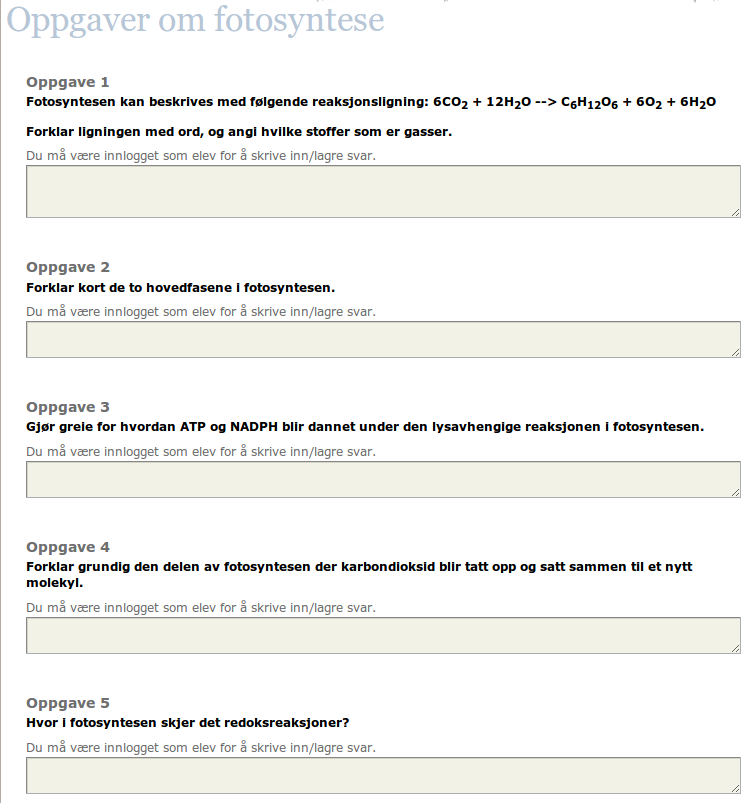
\includegraphics[width=1\textwidth]{img/theoretical/vitenassessment.png}
\caption{Screenshot from viten.no showing student-role metaphor}
\label{fig:scrshotviten}
\end{figure}

Likewise \citet{jimenez2000doing} pose that "doing science" has an obstacle named "doing school". Where "doing science" refers to argumentation or dialog characterized by “construction, representation, evaluation of knowledge claims and investigative methods” \citep{jimenez2000doing}. While "doing school" refers to what actions and activities students and teachers do that instantiates rituals, routines and expectations in educational settings, e.g. review homework assignments, take lecture notes, take tests, complete lab activities etc. \textbf{OBSOBSOBSOBS! DET ER EGENTLIG IKKE JIMINEZ SOM ER PROBLEMET I NESTE SETNING, DET ER DIV ANDRE STUDIER SOM FOKUSERER PÅ DOING SCIENCE OG UTELATER DOING SCHOOL BLABLABLA (SE FURBERGLUDVIKSEN 2008)} \citeauthor{jimenez2000doing} have contributed to the understanding of students argumentation and knowledge claims, but as \citet*{furberg2008students} suggests; a more holistic view is needed to get a rich understanding of the complexity of students' meaning making. Meaning that both the dimension of "doing school" and the dimension of "doing science" needs to be taken into account. 

\subsection{Spontaneous and scientific concepts} \label{cha:spontaneous_scientific}
In the early stages of life, children learn for the most part by experience. Skills such as mastering the native language, walking, running are learned through trial and error. This means that the knowledge of a concept is linked to the concrete experience where she was presented with the concept. A child who is presented with the concept of "brother" by a pointing gesture towards her brother, will at first only associate the word "brother" with that specific person. This is what Vygotsky calls \emph{spontaneous concepts}

An only child on the other hand, will be introduced to the concept of brother through other concepts. A parent can for instance say that "brothers are boys who have the same parents". The concept of brother will then be a general concept for the child, not linked to any concrete experiences, but to the concepts of "boys" and "parents". This is what Vygotsky calls \emph{scientific concepts}

The major difference between these two types of concepts is that spontaneous concepts are developed outside the conceptual framework and only linked to concrete experiences in the mind of the learner. If we presented the child having a brother with the abstract problem of a "brother's brother" \citep{vygotsky2012thought} he would become confused, as his only knowledge of the concept of brother is with situations with his brother

In contrast, scientific concepts are developed within a conceptual framework. They are immediately given a place within the system of concepts, i.e explained by their relation to other concepts. As a result, the child is consciously aware and able to reflect on the concept \citep{van1998concept}. If we presented the only child with the abstract problem of a "brother's brother", he would most likely be able to solve it because of the concepts relation to other concepts in the mind of the child. 

Another example is how children develop a concept of time. In the early stages of life, a child may think that day and night is analogous to light and darkness. This is the spontaneous concept saturated by experience. It is only later in school he learns the scientific concepts of the earth's rotation and its relation to the sun and the moon, which marks days and years. This information has not been appropriated by experience, as the child has not been to space and experienced it, the information is constructed using different signs linked together by the instructor. 

\begin{figure}
\centering
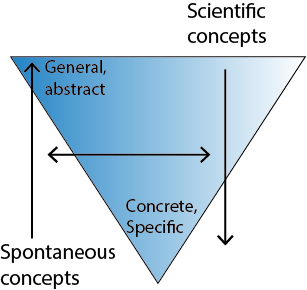
\includegraphics[width=0.6\textwidth]{img/theoretical/conceptpyramid.png}
\caption{The concept pyramid}
\label{fig:conceptpyramid}
\end{figure}

The relationship between these two categories can be explained as an upside-down pyramid. On the top we have the scientific concepts, which are general and abstract. And on the bottom we have the spontaneous concepts, which are specific and concrete. The concepts then move towards each other. The scientific concepts move downwards "toward greater concreteness" in a deductive manner, whereas the spontaneous concepts move "upward toward greater abstractness" \citep{vygotsky2012thought} in a inductive manner.

Even though the concepts move in opposite directions, there is a mutual dependency between them. In Vygotski{\u\i}'s terms: "In working its slow way upwards, an everyday concept clears a path for a scientific concept and its downward development". This means that "the development of a spontaneous concept must have reached a certain level for the child to be able to absorb a related scientific concept" \citep{vygotsky2012thought}. It is therefore essential for the teacher to bring the spontaneous concepts up to a level that makes the scientific concept within reach for the student. By doing this, the student will have the experience, and the related concepts necessary for constructing knowledge of an abstract concept. 

This brings us further to the zone of proximal development, as students who lack consciousness and control over the spontaneous concepts can "find this control within the zone of proximal development" \citep{vygotsky2012thought}.

\subsection{Zone of Proximal Development}
Lev Vygotski{\u\i}, was concerned with the relationship between learning and development, and argues that the theorists of his time such as Piaget, James and Koffka does not provide an adequate view of this. He finds that learning and development are interrelated, and that this relationship has some specific applications in school-learning. \citep[p. 84]{vygotskiui1978mind} Thus, in order to describe these issues he introduces the concept Zone of Proximal Development (ZPD), and defines it as follows:

\begin{quote}“The distance between the actual developmental level as determined by independent problem solving and the level of "potential development" as determined through problem solving under adult guidance or in collaboration with more capable peers” \citep[p. 86]{vygotskiui1978mind}
\end{quote}

The actual developmental level is in other words determined by looking at what a person can do alone. Vygotski{\u\i} found that this traditional way of determining a person's mental development did not hold in school learning, as it only describes what functions in a person that have already been matured. He therefore introduces a new developmental level, the "potential development", which can describe the functions in a person that are in the process of maturation. The actual development of a person is therefore the end product of developing, while the potential development is the state and process of developing. The ZPD can be used as a tool by teachers and instructors to delineate the immediate future of their students, i.e., their actual development of tomorrow.

Vygotski{\u\i} proposes further that ZPD is an essential feature of learning, which distinguishes learning from development, but at the same time provokes developmental processes that would not be possible without learning. In other words,

\begin{quote}“It awakens a variety of internal developmental processes that are able to operate only when the child is interacting with people  in  his  environment  and  in  cooperation  with his peers.” \citep[p. 90]{vygotskiui1978mind}
\end{quote}

By applying the ZPD to learning-situations, the key takeaway is that the analysis alters the traditional view of knowledge or mastery, and shows that the constructed knowledge provides the basis for further development. A great example of this is the process of mastering native language, which initially is learned as a means of communication between the child and other people. The use of language first happens on a social level, in the interaction with people, and is later developed to internal speech and becomes a means to organize thought, i.e., an internal mental function . Vygotski{\u\i} calls this concept the \textit{duality of learning} \citep{vygotskiui1978mind}. 

Another classic example is that of a child trying to grasp a ball. At first the gesture means nothing to the child, but when the mother realizes that the gesture indicates something, the situation changes dramatically. When she gives him the ball, as a result of the hand gesture, the "grasping movement changes to the act of pointing" \citep{vygotskiui1978mind}. This means that the operation that was initially an external activity is now "reconstructed and begins to occur internally" \citep{vygotskiui1978mind}. Thus, \textit{externalization} precedes \textit{internalization}. 

With this in mind, a teacher can understand what developmental processes is maturing in their students, and from that give adapted challenges, show partial solutions and in general tailor what to say and teach next. From this perspective, development is lagging behind learning, and the challenge for the teacher becomes to teach ahead of development, but at the same time not too far ahead. This leads us to the concept of scaffolding, which can be argued to be a refinement of ZPD. 

\subsection{Scaffolding}
Vygotski{\u\i}'s Zone of Proximal Development is the distance between what a person can do alone and what he can do with help from a More Knowledgeable Other (MKO). What types of help and how the MKO should provide it, has not been a focal point for Vygotski{\u\i}. Although \citeauthor*{wood1976role} does not reference to any Vygotski{\u\i}an literature, the term scaffolding introduced by them in 1976, bears resemblance to the very idea of ZPD. As they put it:

\begin{quote}“Scaffolding consist essentially of the adult ‘controlling’ those elements of the task that are initially beyond the learner’s capacity, thus permitting him to concentrate upon and complete only those elements that are within his range of competence” \citep{wood1976role}
\end{quote}

Thus, scaffolding can be applied by MKOs in order to keep the learning process within the learner’s ZPD. There is a is a nuanced balance for how much guiding is needed and a key point is that a person's ZPD is personal, thus a scaffold should be personally adjusted. An example can be if we were to teach two persons how to take a picture with a professional DSLR camera, one being an old woman (Mary) with little insight in technology, the other a young man (Ryan) who has grown up with technology. It is obvious that the two persons have different cultural backgrounds and taking a picture have different meanings to them, hence the tutoring of them need to be differently tailored. In the following section we will go through the six steps of scaffolding provided by \citet{wood1976role} using this example.

\begin{enumerate}
\item{} \emph{Recruitment} - We need to get the learners attention and interest in the task at hand. In our case this could be to show nice pictures of Mary's grandchildren to make her interested in taking nice pictures of them herself. For Ryan we could show the difference between pictures taken with an iPhone and a DSLR camera to make him understand the value of using a DSLR versus his iPhone.

\item{} \emph{Reduction in degrees of freedom} - The task must be narrowed down in order to provide a clear goal that can be reached. For Mary we can say that her task is to take a photo of her grandson playing in the garden with the use of auto-mode. And for Ryan, the task could be to take a landscape photo of his favorite view for his Facebook cover photo with the camera setting called A for aperture, which lets him control the depth of field - an important setting when photographing landscapes. 

\item{} \emph{Direction maintenance} - The learners must be kept on the path towards the goal, which implies a focus on motivation. Both to maintain progression and to keep a focus on the goal. From this point, scaffolding becomes an improvisation skill and it can be hard to plan ahead because of all the unforeseen things that can happen. Ryan can for example stop focusing on the landscape photo and instead take pictures of a car. While Mary starts looking at the pictures contained on the camera's memory stick. In this case one has to evaluate the goal versus the reduction in degrees of freedom. It might be that Ryan is more interested in taking pictures of cars, and since the main goal is to learn to take photos with a DSLR camera, an adjustment of the end product can be done. In Mary's case however, she might be easily distracted, and just needs someone to tell her to focus on taking pictures of her grandson. These are nuances that can be hard to spot, and requires a tutor with good improvisation skills.

\item{} \emph{Marking critical features} - Marking what the learner has done versus what is expected. This could be to show Mary that in her picture, she has left half her grandson's head out of the picture, and that she should try to capture a photo with the whole face visible. For Ryan it could be to point out that he has a very small depth of field in his photo, putting the trees in the foreground into focus, while leaving the mountains in the background blurred. Examples of correct solutions could be used to demonstrate the discrepancies between what the learner has produced and a correct solution.

\item{} \emph{Frustration control} - Balancing the dependency of the tutor and the independent problem solving. Both Mary and Ryan should be given some space to try taking photos, but we should at the same time be observant of when guiding or telling is needed. We could tell them to have the sun behind them to get the right light conditions, and hold the camera with two hands. The major risk here, is that the learner can become too dependent of the tutor, making it harder for the learner to achieve the goal, i.e. taking a picture alone at a later time.  

\item{}  \emph{Demonstration} - Showing a solution to the task, imitating the learner's earlier attempts and possibly correcting errors, with a hope that the learner will imitate back in a more correct manner. For Mary we could take a picture of her grandson, imitating her position, look for the sun, and then correct the position to get the sun behind us. Or for Ryan we could place the camera on a chair and use a timer to reduce movement in the camera, thereby allowing a slower shutter speed, which again allows a higher aperture, increasing the depth of field, giving focus to both the trees in the foreground and the mountains in the background. This might be supplemented by telling, to provide a context to the tutor's actions.
\end{enumerate}

As presented, some of these steps require planning while others require improvisation. Both the planning and improvisation turns out to be tailored to the specific situation at hand with all the complex contexts the learners bring with them to the situation. The steps can either be carried out manually by a tutor, or be mediated automatically by a computer-based system. \citet{fischer1991critics} presents one implementation of a computer-mediated scaffold where a critiquing system gives the user a "reasoned opinion about a product or action generated by a human". Another example is from \citet{furberg2009socio} where prompts requiring user-input is used to promote student reflection. 

One important thing to note when reviewing the literature on scaffolding by \citet{wood1976role} and ZPD by \citet{vygotskiui1978mind} is that these studies are done on pre-school children. Critics may therefore argue that the concepts are not applicable to adult learning. Our stance is that when learning new concepts, both children and adults are alike. New and unknown concepts are new and unknown both for adults and children, and adults therefore become "as children" when introduced with new learning material. The concepts can therefore be used to analyse learning in all contexts where learning takes place. 

%Even though the six steps provided by \citet{wood1976role} can be considered as a framework for scaffolding, it is still quite complex and demands careful consideration by the teacher or the designers of the computer based scaffold.  

\section{Multiple External Representations}
Multiple external representations (MER) have been used since long before the advent of computers for conveying information. Textbooks and manuals often contain images and illustrations, maps show different information in different ways, and whiteboards are used in addition to speech. With digital technology the possibilities of MER are expanded to include dynamic linking between the representations, and the representations can show dynamic information that is not available in the real world, e.g., showing the flow of oxygen. 

In an effort to identify the features of MER, \citet{ainsworth1999functions} has developed a classification framework. She suggests that MER can serve primarily three different purposes in learning situations:
\begin{itemize}
\item{} \emph{Complementary roles} - Different representations can focus on different aspects of the phenomenon under study, or they can contain different information of the same phenomenon. E.g. a topographic map in addition to a road map. 
\item{} \emph{Constrain interpretation} - One representation can be used to constrain the interpretation of the other. E.g. the text “the fork lies next to the spoon”. It is impossible to tell which side the fork is on, but by presenting an illustration of the example, the representation will constrain the interpretation of the text. 
\item{} \emph{Construct deeper understanding} - MER can be used to “promote abstraction, to encourage generalization and to teach the relation between representations” \citep{ainsworth1999functions}. 
\end{itemize}

The three different roles presented above are also the benefits of using MER. Complementary roles can support students to make up for insufficient knowledge of one representation by using another, constrain interpretation can “support the learners’ reasoning about the less familiar representation” \citet{ainsworth1999functions}, and finally the learners can gain deeper understanding of the domain by translating between representations \citep{van2006supporting}. 

On the other hand, when learners are faced with MER they must also undertake additional tasks as to understand the phenomenon or domain in question. This may lead to a heavy cognitive load, which “may leave less resources for actual learning” \citetext{Sweller, 1988, 1989, referenced in \citealp{van2006supporting}}. A key issue is then to reduce the cost for learners associated with MER, while keeping the benefits. 

\section{Inquiry learning}
According to \citet{prince2006inductive} science has traditionally been taught in a \textit{deductive} manner. In the same way as Sherlock Holmes collects piece by piece to form a theory, the students collect pieces of models and illustrations to grasp a scientific concept. Little attention is paid to why the students should learn the material, apart from having to perform on tests.

On the other hand we have the \textit{inductive} ways of teaching and learning. Instead of beginning with the theory, the students are presented with some sort of task, which becomes the motivation to learn the tools required to solve the task. Examples of this can be to make a battery in a science class, or finding out why potato-chips bags seem more inflated on the top of a mountain than by the sea.

Inquiry learning involves giving the students "questions to be answered, problems to be solved, or a set of observations to be explained" \citep{prince2006inductive}, or in other words: giving the students incentives to ask for information. There are several other inductive learning methods, such as problem-based learning, discovery learning and project-based learning, which all can be explained with the same statements as inquiry learning. Inquiry learning can therefore be seen as an umbrella term for inductive learning methods. \citep{prince2006inductive}

\citeauthor*{staver1987analysis} \citetext{\citeyear{staver1987analysis}, referenced in \citealp{prince2006inductive}} differentiates between \emph{structured inquiry} (e.g. tutorials), \emph{guided inquiry} and \emph{open inquiry}. This relates to the ZPD and scaffolding. Depending on the student's developmental level, different framings of the inquiry process are needed. To scaffold the inquiry learning process is not an easy task. In a review article, \citet{de1998scientific} identify four problems that learners may encounter when engaging with inquiry learning: \textit{hypothesis generation}, \textit{design of experiments}, \textit{interpretation of data}, and \textit{regulation of discovery learning}. They continue to argue for the need of supporting students during the process of scientific inquiry, providing scaffolds for each of these problems. The challenge then becomes "guiding students to the “right” path, but at the
same time letting them discover and make the discovery their own." \citep[p. 247]{kluge2010simulation}. In other words the students need to be steered towards the interesting discoveries, but at the same time have the freedom to explore and not be commanded in any way.

\subsection{Misconceptions}
Misconceptions appear in most educational contexts. According to \citet{gomez2008elementary} students have "qualitative differences in his or her understanding of science that is often inconsistent with what the teacher intended through his or her instruction". These are often deeply rooted, and remain intact even after instruction. This becomes especially relevant when dealing with inductive learning methods, as the students are given more freedom to explore their own ideas, and thus more freedom to pursue tracks that may lead to different conclusions than the ones intended by the instructor.

The term itself has been given many labels in research literature, depending on the focus: "alternative frameworks", "preconceptions", and "student ideas" are just some of them. An important factor here is how misconceptions are perceived. Are they resources for learning, or obstacles that the learner has to overcome? If we look at meaning making from a constructivist point of view, advanced knowledge is built upon prior understanding. Misconceptions then become "faulty extensions of productive prior knowledge" \citep{smith1994misconceptions}.

To then simply write misconceptions off as mistakes is, according to \citet{smith1994misconceptions}, a too narrow view in their role in learning. If we take the example of stating that "multiplication makes numbers larger", it is indeed an accurate explanation of most multiplication pieces. The problem arises in the few cases where we multiply by non-natural numbers. The conception that leads to erroneous conclusions in some contexts can be quite useful in others \citep{smith1994misconceptions}. The misconceptions are therefore for the students "conceptions in their own right with plausibility and at explanatory power" \citetext{Smith, diSessa \& Roschelle 1993, referenced in \citealp{larkin2012misconceptions}}. 

%As stated before, the goal then becomes to scaffold the students in such a way that the interesting discoveries are made, and the misconceptions discussed. 

\section{Summary of Concepts for Analysis}
We have now introduced the Sociocultural perspective and several important concepts within and besides its frames. Further we will use the Sociocultural perspective and the following concepts to guide our research design and discuss our findings:

\begin{itemize}
\item{Zone of Proximal developement (ZPD)}
\item{Scaffolding}
\item{Misconceptions}
\item{Multiple external representations (MER)}
\item{Institutional settings}
\item{Inquiry learning}
\item{Everyday language \& Scientific language}

\end{itemize}
 %!TEX root = ../document.tex
\chapter{Empirical settings and methods}
In this chapter, we will present the empirical setting and methods used in this thesis. First we will describe the empirical setting in which the data collection took place. Then we will proceed to present the methods for gathering data with a description of the technicalities of the data. Lastly, we will describe the procedures for selection and analysis of data.

\section{Case Study}
%vet ikke helt hva jeg har starta her, tror jeg må lese noen oppgaver med casestudy.
In our thesis, we have chosen gather data through a qualitative case study.  One of the most important reasons for choosing a case study was as \citet{yin2003case} states: "you want to cover contextual conditions because you believe they are relevant to the phenomenon under study". As the case was students inquiry about photosynthesis, it could not be examined without the context, the school, or more precisely the biology classroom setting where Monoplant was inserted. 



\section{Empirical setting}
The collection of data material used in this thesis took part in late autumn 2013, at a high school located in the center of Oslo. The school has a high threshold for admission, with a lower requirement of 43.5 points out of 60 in 2010 \citep{utdanningsetaten}. Thus, the students at this school are (mostly) high achievers. 

Contact with the school was first initiated through Intermedia, and a presentational flier was sent as an explanation of the project (see chapter \ref{samtykkeskjema}). A teacher contacted us, and luckily our request coincided perfectly with a two-week time frame for reviewing photosynthesis in his biology class. The teacher was therefore willing to test out our application instead of performing one of the experiments described in the textbook. 

The class selected was a biology class at the highest level offered at the school, biology 2, which has an extensive curriculum covering e.g. photosynthesis, enzymes and energy transmitters \citep{bios}. The class consisted of 11 girls and three boys between 17 and 18 years of age (vg3). For the main part of our data collection, all of the students were present. All of them agreed to participate in the study, but due to technical limitations and a busy time schedule, the primary data collection was  done with a small sample of the group. 

\subsection{Ethics}
Prior to the data collection, an application was sent to NSD (Norwegian Social Science Data Services) requesting permission to film the students. The application was approved with only minor changes to how the material was to be treated after completion. In addition all the students taking the class were given an consent form stating that participation was voluntary, and all material would be kept anonymous (see appendix). 

Throughout this thesis, and in the transcripts of video data, all the students' names have been replaced by pseudonyms and the name of the school is never mentioned. The data material containing identifying information of the students has been and will be stored securely on a separate hard drive at Intermedia, and will be deleted  upon termination of the project. 

During our time at the school we were always open about our role as researchers, and explained on several occasions how the data was going to be used. 

\subsection{Planning the experiments}
An initial planning and presentational meeting was held on the 21st. of October with the teacher. A thorough presentation and demonstration of the system was given, along with a discussion of the functionalities of the system, to see if it would spark some ideas for experiments. 

Stressing the importance of a scientific method, the teacher suggested that we could conduct two experiments, using the different sensors in the system to change one variable, while keeping the others relatively controlled. We agreed that the factor that would be easiest to control, yet yield interesting results was light intensity and light quality (wavelength). The first experiment would involve keeping the plant located in a window facing west, receiving sunlight and light from the fluorescent indoor-lighting, while we in the second experiment would relocate the plant to a light proof cabinet where it would only receive light of a known wavelength. Each of the two experiments would span a one-week period, depending on the time needed for measurable results.

\subsection{The experiments}
The project was presented for the class during a one-hour lecture on Friday 25th of October. We used the opportunity to give an in-depth explanation and demonstration of Monoplant, as well as explaining how we would collect and use the data material gathered. We then proceeded to initiate the first experiment, which went on for seven days until Friday 1st of November when the second experiment was initiated. The second experiment went on for 13 days until Wednesday 13th of November when the primary data collection session took place. During the experiments we as observers and researchers were present at four separate occasions, observing what the teacher was focusing on, and the nature of the class discussions. In addition we answered any questions they had regarding the system, and observed how it was used by the teacher and how the students interacted with it. 

\begin{figure}
\centering
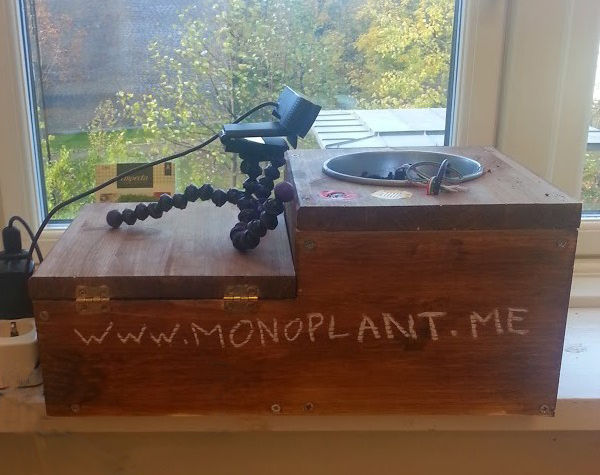
\includegraphics[width=0.8\textwidth]{img/empiricalsetting/window.jpg}
\caption{The experimental setup located in the window}
\label{fig:windowplant}
\end{figure}

\begin{figure}
\centering
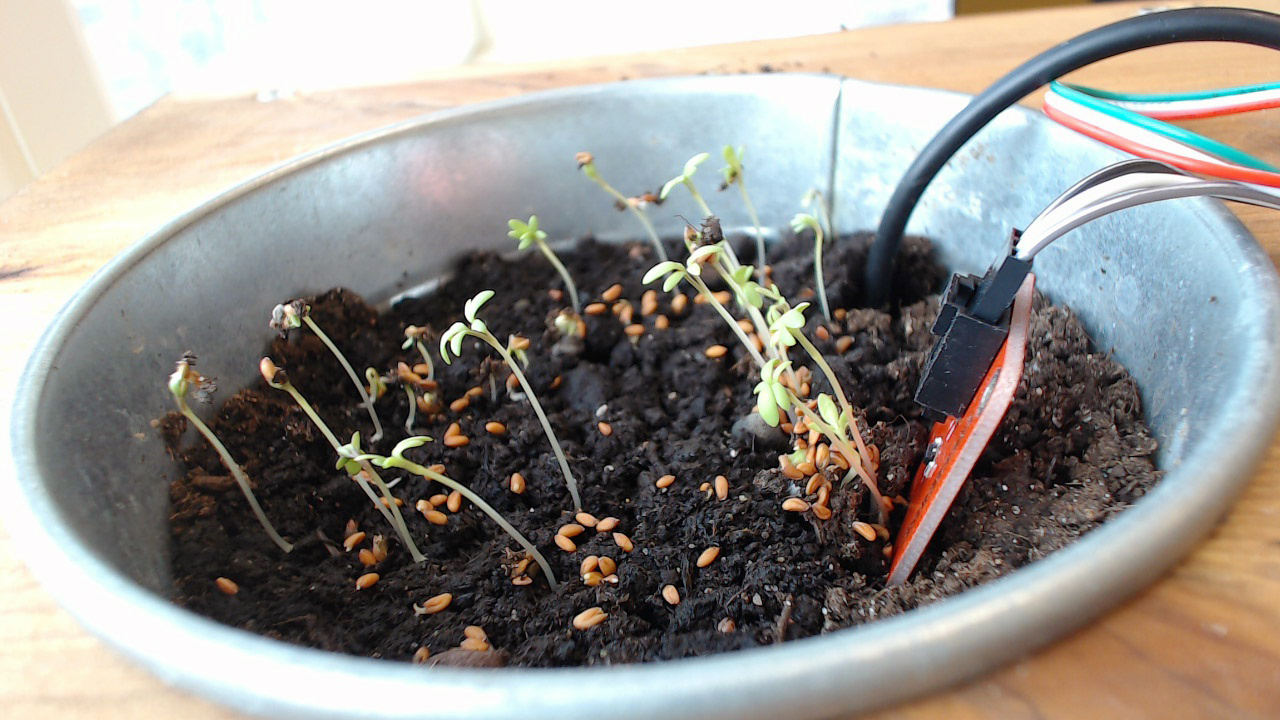
\includegraphics[width=0.8\textwidth]{img/empiricalsetting/windowsystem.jpg}
\caption{The plant receiving natural light}
\label{fig:windowsystemplant}
\end{figure}

\subsubsection*{The plant in the window}
The first experiment was conducted with a setup in the window as shown in figure~\ref{fig:windowplant}. The system was located in the front of the classroom near a door leading to the adjacent classroom, visible and in reach of everyone walking by. As figure~\ref{fig:windowsystemplant} shows, there is between 50 and 70 seeds in the pot. The plant was located in the window sill, exposed to sunlight or daylight depending on the weather, in addition to the fluorescent indoor-lighting. Due to the time of year, and lack of people using the classroom in the evening, this meant that the plant would get light in the period between 08:00 and 17:00.

It turned out that the system was draining power from a power outlet that was either connected to the indoor light or timer based, as the system went down and did not post data between 19:00 and 07:00. We also had some technical issues with the system from 25th of October to 27th of October, resulting in lost data from the first seeds germinating.

\begin{figure}
\centering
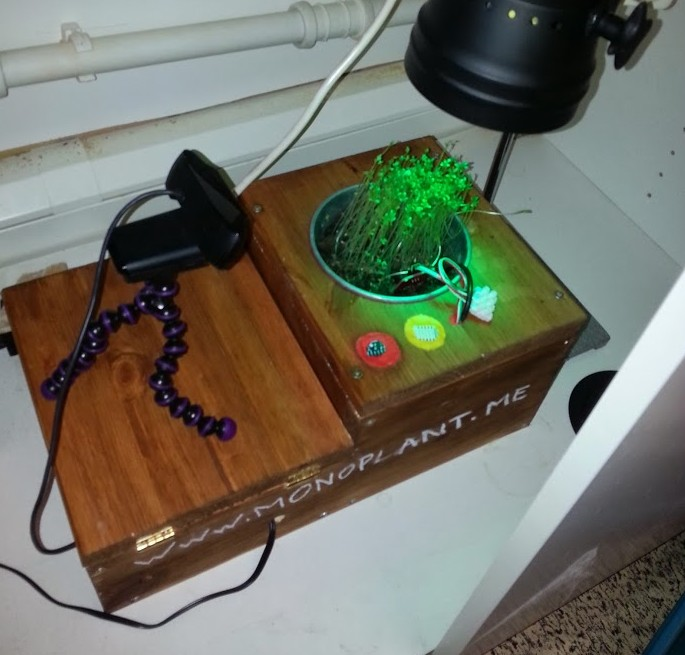
\includegraphics[width=0.8\textwidth]{img/empiricalsetting/cupboard.jpg}
\caption{The system located in the cabinet}
\label{fig:cabinetplant}
\end{figure}

\begin{figure}
\centering
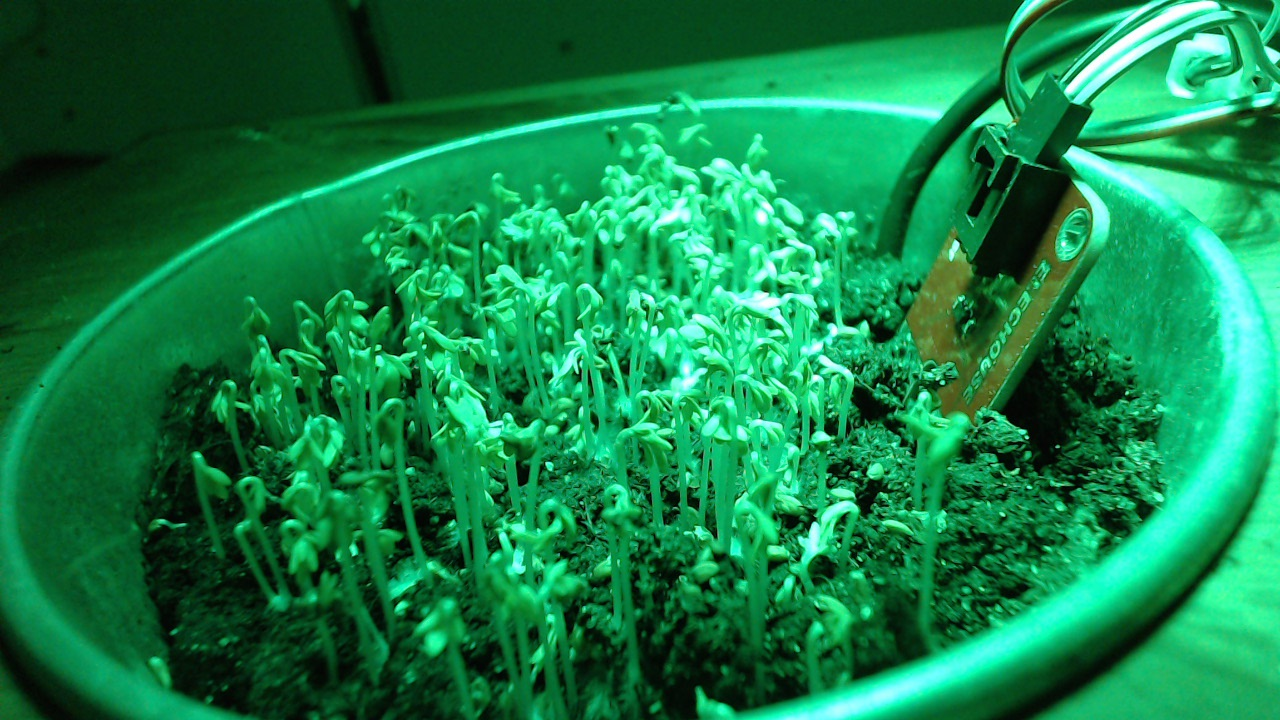
\includegraphics[width=0.8\textwidth]{img/empiricalsetting/cupboardsystem.jpg}
\caption{The plant in the cabinet, receiving green light}
\label{fig:cabinetsystemplant}
\end{figure}

\subsubsection*{The plant in the cabinet}
The second experiment was conducted with a setup in a cabinet as shown in figure~\ref{fig:cabinetplant}. The cabinet was located in a corner in the front of the classroom behind the teacher's desk, hidden and not nearly as accessible as the plant in the window. The picture in figure~\ref{fig:cabinetplant} is taken with light from the room coming in to the cabinet, hence it does not reflect the lighting conditions in the cabinet during the experiment. The cabinet door was closed and the lamp above the plant was emitting green light 24 hours a day, hence figure~\ref{fig:cabinetsystemplant} shows the lighting conditions more correctly. It is also worth noting that the pot contains around 30-40 seeds more than in the first experiment. When this experiment took place we did not have any technical issues, the system posted data continuously for the whole period.


\section{Methods}
Different methods for data collection was discussed and reviewed early on in the project. Our most influential source, regarding paradigm, methodology and method was the tradition for using qualitative data in information systems research in the design group at department of informatics. As our primary data source we chose video data with the use of multiple cameras and a screen dump. This was collected during a 45-minute session after the completion of the experiments, resulting in 3x45 minutes of video data and 45 minutes of audio data. Supplementary data from this session includes the written answers from the groups that were not filmed, and our personal notes. In the following sections the methods used will be discussed. 

\subsection{Video and audio}
It was determined early in the project that video and audio recording were to be used. The primary reason for this was the tradition at Intermedia, as video data collection has been used and thoroughly tested by a number of researchers here. This meant that we would get a lot of help from co-located researchers in what microphones to use, placement of cameras, operation of the equipment, etc. 

A total of 45 minutes of video and audio was recorded, using three separate video sources, and three microphones. One camera was placed in front of the group, able to capture facial expressions and where the students were looking. This camera had an external microphone connected that we placed on the table in front of the students, allowing us to filter out some of the noise in the classroom. The second camera was placed behind the students on their right hand side, facing the computer screen. This camera's primary function was to capture where the students were pointing and what they were doing on the laptop. The audio source of the second camera was the built-in microphone, which proved to cover most of the audio in the classroom. In addition to the video cameras we recorded a screen capture from the laptop, showing exactly what the students were doing in the system. The laptop had a built-in microphone as well but we only used the sound from camera two and the laptop to synchronize the different videos.
\begin{figure}
\centering
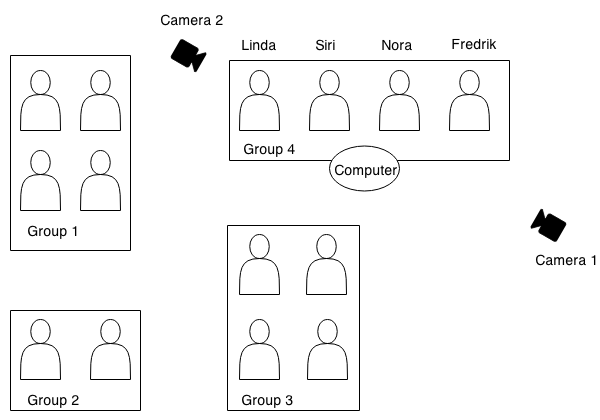
\includegraphics[width=0.8\textwidth]{img/empiricalsetting/class_diagram.png}
\caption{Camera setup}
\label{fig:camerasetup}
\end{figure}

\subsection{Passive observation}
During the experiments we were present at four separate occasions. The primary reason was to ensure that the system was working, assist with any technical difficulties regarding the user interface, and to ensure a smooth operation of the experiments. But we would also take notes regarding how the system was used in the lecture, if or how students showed interest in the experiments, and how the teacher was conveying information about photosynthesis in general. While these observation sessions were not thoroughly planned, and the data material never systematized, it proved to be a good supplementary data source to help us structure and make sense of our primary data. We would later on also use these notes as discussion points and indexical resources when reviewing the data material. 

\subsection{Student produced material}
While we filmed the group of students selected for our main data gathering, the rest of the class was divided into groups and told to discuss and write down answers to the given assignments. These answers were handed in and rewritten into computer documents later (see appendix X). This became a fine supplemental data source, as it gave an insight of what answers fellow students of the class came up with in a less monitored setting. 

\subsection{Web logs}
In order to review activity on the web page (\url{http://Monoplant.me}), Google Analytics tracking system was installed. Although we did not use this extensively, it allowed us to see if and how often the system was used, and if students were using it at home or only during classroom hours. 

\section{Analytical Procedures}
From mid November till late December 2013, we were observing, listening, transcribing and discussing the material. In this section we will discuss how we approached, selected and made sense of the data once it was collected.



\subsection{Approaching the data}
\citet{derry2010conducting} speaks about two different approaches to select parts of a video corpus for further examination: the \emph{inductive} and the \emph{deductive} approach. Inductive approaches apply when a minimally edited video corpus is collected and investigated with broad questions in mind but without a strong orienting theory. Deductive approaches involve identifying or creating a suitable video corpus and systematically sampling from it to examine specific re-search questions. \citep{derry2010conducting} To start with, we clearly fit into the inductive approach, but as many researchers have experienced: once you find something, you start looking for it. Hence our approach became leaned more to the deductive side later in our analysis.

To make sense of the data gathered we looked at it in several different ways with different focuses. Below is a chronological list of the ways we approached the data. 

\begin{enumerate}
\item{Initial screening of main video corpus, locating interesting interaction}
\item{Transcription of main video corpus}
\item{Watching supplemental video material to make detailed notes on interactions with the system}
\item{Watching the main video corpus with our supervisor and discussing which events and interactions are interesting and/or can be explained by existing theory}
\item{Select parts of transcript that are of interest}
\item{Detailed transcriptions of these parts}
\item{Writing explanations for these interactions}
\item{Linking interactions to support each other}
\item{Cut excerpts that did not fit together with other excerpts}
\item{Linking chunks of interactions to related theory}
\end{enumerate}

While we still had the impressions from the data collection fresh in mind, we sat down and watched all the video material. During the screening process we tried to make a content-log to get a better overview of a large corpus of data and select cue points in the video where interesting interaction took place, focusing on change in context and contradictions. This was followed by a rough transcription, using mostly audio and video from the camera facing the students. At this point we focused mostly on transcribing what was said, not paying attention to small audible details such as intonation. 

We then went on to the third step in the process, bringing in additional video material to generate thick descriptions of the interesting interactions taking place. Using audio cues, we merged all the three video files into one, so that the screen was divided into three parts: one for the camera facing the students, one for the camera facing the screen, and one for the screen dump. This enabled us to make a more detailed transcript of the parts containing inaudible utterances.

At this point in the process we presented the transcript and screened the video along with our supervisor, marking the points in the video that we deemed most interesting. In the following discussion a list of themes or grouping categories was selected, which would be subject to further analysis. A selection of excerpts from the transcripts was then picked out for further analysis where we kept focus on intonation, gestures, etc. to provide a thorough description of the events unfolding. 

As shown in the list, our approach was quite open to begin with, scanning the complete video corpus for what we found interesting. Once we began to find parts that interested us, we started to look for similar events and contradicting events. With help from our supervisor we found theoretical concepts we could link to our material, which again gave us an incentive to look for a specific type of material.

\subsection{Interaction analysis}
%Crang & cook: Video recordings can be criticized by pointing out that it is the researcher that selects the frame and focus. Hence the data can become biased. However, by trying to frame interaction generically, and providing a video, getting other people to double check coding and transcription.
The analytical procedure employed within this thesis is \emph{Interaction analysis} \citep{jordan1995interaction}, which emerged from fields such as ethnography, sociolinguistics, ethnomethodology, conversation analysis, and sociocultural theories. \citeauthor{jordan1995interaction} describes it as follows:

\begin{quote}
An interdisciplinary method for the empirical investigation of the interaction of human
beings with each other and with objects in their environment. It investigates human
activities such as talk, nonverbal interaction, and the use of artifacts and technologies,
identifying routine practices and problems and the resources for their solution \citep[p39]{jordan1995interaction}
\end{quote}

For Interaction analysis to become a reality video and audio recording technology has been a vital resource. The combination of recording talk as well as nonverbal interaction and the ability to replay a sequence as many times as necessary gives us the possibility to analyze more thoroughly. Combining this micro-level data of interaction with ethnographic data gives us a means of analyzing how the interaction is part of the situated context and institutional practices. \citep{furberg2009scientific}. 

\subsection{Systemic vs. dialogic}
\citet{arnseth2006approaching} introduces a distinction between two approaches to CSCL research: \emph{systemic} and \emph{dialogic}. A main feature of studies characterized to be using a \emph{systemic approach}, is that they generate models of how features of the technological system reviewed affects reasoning, collaboration, structures of discourse etc. The analytical focus is on describing the systematic relations between forms of social interaction, and specific types of support or other contextual factors on the one hand, and qualities of outcome on the other. \citep{arnseth2006approaching} In other words, \emph{systemic} studies tend to measure how much a specific feature or configuration in a CSCL-tool affects learning outcomes in terms of "measurable" or "quantifiable" variables. The result of this analytical practice is often a formulation of a model or reformulation of an existing model, which may state that a CSCL application together with a certain practice, are likely to produce a positive learning outcome.

\citeauthor*{arnseth2006approaching} argue that there has been little interest in the emergent characteristics of actions that take place when CSCL-tools are introduced in schools. As they write: \emph{"we need to examine more closely how the meaning and functions of CSCL applications are actually constituted in practice."} \citep[p. 181]{arnseth2006approaching}. Hence they introduce the \emph{dialogic} approach, where CSCL applications are not treated as a variable with features and configurations that in relation to other variables i.e. learning outcome can be determined statistically. Instead, the analytical concern  of the \emph{dialogic} approach is with how computer applications provide a new context for social interaction.

%\sout{ By observing the class during our visits to the school during the experiments, and by reading the textbook chapter on photosynthesis, we gathered ethnographic data on how the class worked together and what they were expected to know about photosynthesis. }

%\sout{Even though we have done a case study in a real educational setting, considering these ethnographic data is important if we are to keep a dialogic perspective.}


%\sout{At point 8 in the list, we had found over 20 excerpts that we wanted to present and discuss. By categorizing these into four themes: \emph{Hypothesis generation and testing}, \emph{Misconception}, \emph{Conceptualization} and \emph{Linking between representations}, we were able to find the best excerpts to represent the themes. Hence we ended up with 11 excerpts, which will be presented in the following chapter.}

 %!TEX root = ../document.tex
\chapter{Data \& Analysis}
In this chapter we will present the findings from our case study with a focus on themes relevant to our research questions. Each of the themes contain at least one Excerpt with a context description, excerpt from the transcript, and an analysis of the unfolding events. 

The first theme (\ref{cha:hypothesisgeneration}) is named \textit{Hypothesis generation and testing}. Here we follow a hypothesis from generation to falsification to a new improved hypothesis. Then we move on to \textit{Misconception} (\ref{cha:guidedinquiry}) where we show examples of how misconceptions can be addressed successfully or unsuccessfully by the teacher, and how it can lead to hypothesis generation based on false premises. The third theme (\ref{cha:conceptualization}) is dubbed \textit{conceptualization} and presents three Excerpts regarding scientific and everyday language. The last theme (\ref{cha:linking}), \textit{linking between representations}, aims to show how the students relate the digital representation to the physical world (biology of plant).  

For the sake of simplicity the first experiment, where the plant was located in the window has been named plant A, and the second experiment where the plant was located in the cabinet, plant B. 


\begin{table}[H]
\begin{center}
	\begin{tabular}{l r r } \toprule
	Who &  Interactions  & Percentage\\ \midrule  
	Linda &	 14  & 3.67\% \\
	Nora&	118 & 30,97\% \\ 
	Siri& 	182 & 47.77\% \\
	Fredrik& 67 & 17.59\% \\ \midrule
	All &	381 & 100\%\\
	\bottomrule
	\end{tabular}
\end{center}
\caption{Verbal interactions by participant}
\end{table}

\section{Hypothesis generation and testing}
\label{cha:hypothesisgeneration}
\subsection{First claim}
\subsubsection*{Context}
\label{firsthypothesis}
We enter the situation at the beginning of class. The students have been divided into groups, and they are approximately two minutes into the task. Preceding this discussion, the students have tried for about one minute to figure out what the task is about, and what the two experiments involved. Siri has read out loud the first question in the assignment: "what did you expect would happen?" (in the experiment), and they have rehearsed some of the theories presented in previous lectures (e.g soil moisture decreasing over time). Prior to the excerpt, the students have appeared a bit insecure about the task. But as we enter the setting they seem more focused and interested, and the discussion has changed from making general observations to generating hypotheses.

\subsubsection*{Excerpt 1}
\begin{table}[H]
	\begin{center}
		\begin{tabular}{r l p{7cm} p{3cm} } \toprule
				Time &  Who &  Speech  & Action \\ \midrule 

			2:04 %time
			&Nora %name
			&\parbox[t]{7cm}{\raggedright hehe.. mm.. hmhm .. når den stod i skapet så.. jeg visste ... %speech 
			}&\parbox[t]{3cm}{\raggedright  %action 
			}
			\\

			2:13 %time
			&Siri %name
			&\parbox[t]{7cm}{\raggedright ... neddi skapet ... %speech 
			}&\parbox[t]{3cm}{\raggedright  %action 
			}
			\\

			2:13 %time
			&Nora %name
			&\parbox[t]{7cm}{\raggedright eller jeg visste ikke helt hva den skull.. hva som skulle skje da egentlig .. %speech 
			}&\parbox[t]{3cm}{\raggedright  %action 
			}
			\\
			2:16 %time
			&Siri %name
			&\parbox[t]{7cm}{\raggedright .. det var det planten stod i skapet også skulle det være bare grønt lys på den ... men det kan jo hende for eksempel at det kom litt annet lys inn i skapet også .. så da er det ikke sikkert at det bare var grønt lys ..  %speech 
			}&\parbox[t]{3cm}{\raggedright peker på skapet %action 
			}
			\\

			2:31 %time
			&Nora %name
			&\parbox[t]{7cm}{\raggedright  %speech 
			}&\parbox[t]{3cm}{\raggedright nikker %action 
			} 
			\\

			2:31 %time
			&Siri %name
			&\parbox[t]{7cm}{\raggedright og planten tar jo opp littegrann grønt lys også, men ikke så mye .. så derfor kunne det hende atte den ikke vokste like my.. eller jeg trodde at den ikke ville vokse like mye i skapet .. siden da fikk den bare grønt lys ...  %speech 
			}&\parbox[t]{3cm}{\raggedright  %action 
			}
			\\
			2:46 %time
			&Nora %name
			&\parbox[t]{7cm}{\raggedright ... mmm ... %speech 
			}&\parbox[t]{3cm}{\raggedright  nikker%action 
			}
			\\
		\end{tabular}
	\end{center}
	\caption{First hypothesis}
	\label{excerpt:hypothesisgeneration}
\end{table}

\subsubsection*{Analysis}
\begin{figure}
\centering
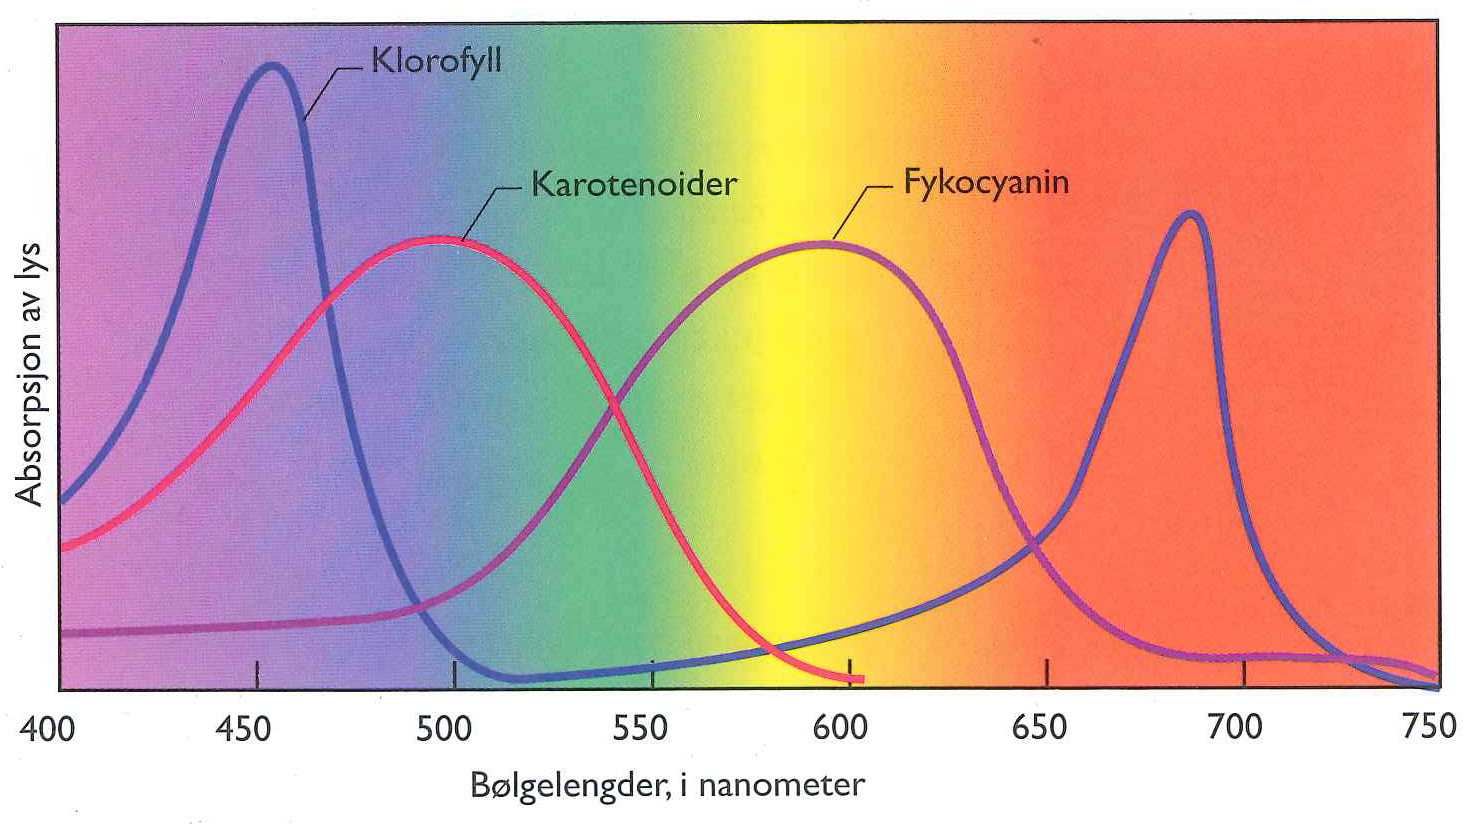
\includegraphics[width=\textwidth]{img/dataandanalasys/absorbtion.png}
\caption{Absorption of wavelengths by pigments \citep{bios}}
\label{fig:absorption}
\end{figure}
At first, Nora is not sure what would happen to the plant given green light in the cabinet (plant B). Siri, as one who thinks out loud, promptly starts reflecting on what could have happened. First she proposes that the plant was given more than green light, indicating that there could be error sources to the experiment. This is acknowledged by a slight nod from Nora. Then she goes on to reflect on the wavelengths plants absorb, agreeing that they only absorb a small amount of green light. They conclude that the plant in the cabinet would not grow as much as plant A. Nora agrees with this hypothesis by nodding and saying "mmm". 

The basis for the statement that plants only absorb a small amount of green light can be found in the textbook: "reflected and transmitted light can hit our eyes and give the object color" \citep[pg. 103]{bios}. The book also contains a graph of the different pigments according to the wavelengths of light they absorb (see fig. \ref{fig:absorption}), clearly showing that chlorophyll absorbs little of green light. In addition, the teacher has used this as a discussion point in earlier lectures, asking why plants' leaves appear green. 

\subsection{Claim refuted}

\subsubsection*{Context}
We enter the setting immediately after the excerpt explained in the previous section. Siri has generated a hypothesis, that she wants to test out. The mood in the group has now gone from laughter and insecurity about the task to concentration and goal-driven work. The overall noise level in the class room has also fallen significantly. 

\subsubsection*{Excerpt 2}
\begin{table}[H]
	\begin{center}
		\begin{tabular}{r l p{7cm} p{3cm} } \toprule
			Time &  Who &  Speech  & Action \\ \midrule 

			2:47 %time
			&Siri %name
			&\parbox[t]{7cm}{\raggedright ...eller nesten bare grønt lys ihvertfall ... men hvor mye vokste den egentlig? er det den ((refererer til planten på bordet)) som stod i skapet? %speech 
			}&\parbox[t]{3cm}{\raggedright peker på planten som står på pulten %action 
			}\\

			2:52 %time
			&Sjur %name
			&\parbox[t]{7cm}{\raggedright ja %speech 
			}&\parbox[t]{3cm}{\raggedright  %action 
			}\\

			2:53 %time
			&Nora %name
			&\parbox[t]{7cm}{\raggedright OJ(!) %speech 
			}&\parbox[t]{3cm}{\raggedright  %action 
			}\\

			2:53 %time
			&Siri %name
			&\parbox[t]{7cm}{\raggedright Den har jo vokst ganske mye %speech 
			}&\parbox[t]{3cm}{\raggedright smiler %action 
			}\\
			2:59 %time
			&Siri %name
			&\parbox[t]{7cm}{\raggedright men var stilkene på den som stod i vinduet var de også hvite? %speech 
			}&\parbox[t]{3cm}{\raggedright Peker mot vinduet %action 
			}\\
		\end{tabular}
	\end{center}
	\caption{Claim refuted}
	\label{excerpt:testinghypothesis}
\end{table}
\subsubsection*{Analysis}
After Siri proposed that plant B would not grow as much as plant A, she wants to find out if it holds. Suddenly she notices the plant, which is placed on the table in front of them, and exclaims, "is it that one(!)?". When Sjur confirms, the whole group and especially Siri look surprised. It seems like they all firmly believed that the hypothesis Siri presented earlier (see section \ref{firsthypothesis}) should hold true. Their knowledge of photosynthesis would also point to the plant not growing as much as it had. Thus, the first hypothesis generated by the group has now been falsified. 

As a reaction to this Siri stops to think for a few seconds before she points at the window and asks: "were the stems on the one in the window also white?". This is a very appropriate scientific question, as a plant with absolutely no photosynthesis would most likely be white, as a result of having no pigments. The reason for her asking this may be related to a comment made by another student in a previous lecture. He had observed that when they put plants in the basement for winter storage, the leaves would turn white. 

\subsection{A new claim}
\subsubsection*{Context}
This next excerpt is from a situation occurring only a few seconds later. The group has been instructed to interact with the system on the computer in front of them to find the answer to the question asked at 2:59 \emph{"were the stems on the one in the window also white?"}. When we enter the situation they have a video of plant A on the screen in front of them, dated 31st of October, ready to play. 

\subsubsection*{Excerpt 3}
\begin{table}[H]
		\begin{center}
			\begin{tabular}{r l p{7cm} p{3cm} } \toprule
					Time &  Who &  Speech  & Action \\ \midrule 
				3:21 %time
				&Nora %name
				&\parbox[t]{7cm}{\raggedright Ja for karse har jo hvit stilk %speech 
				}&\parbox[t]{3cm}{\raggedright  %action 
				}\\

				3:23 %time
				&Siri %name
				&\parbox[t]{7cm}{\raggedright Ja det de har hvit stilk de også %speech 
				}&\parbox[t]{3cm}{\raggedright  %action 
				}\\

				3:24 %time
				&Fredrik %name
				&\parbox[t]{7cm}{\raggedright mhm ... mmja så da er det jo egentlig ganske ... ja ikke så stor forskjell da på de som stod ...  i skapet ((peker på planten på border)) og de som stod i vinduskarmen hvis man bare ser på ...  utseende %speech 
				}&\parbox[t]{3cm}{\raggedright Dette sies mens Siri starter videoen, hun stopper også videoen før de har sett den halvferdig. %action 
				}\\

				3:37 %time
				&Siri %name
				&\parbox[t]{7cm}{\raggedright ja .. men da ville jeg kanskje tenke at det kan hende at det kom inn annet lys enn det grønne lyset også. siden de har vokst så bra, og at de vokser bedre hvis de får flere.. lys i flere bølgelengder enn bare grønt lys %speech 
				}&\parbox[t]{3cm}{\raggedright Stemmeleiet går opp mot slutten av setningen, og løfter blikket fra arket for å få bekreftelse
				 %action 
				}\\
			\end{tabular}
		\end{center}
	\caption{A new claim}
	\label{excerpt:newhypothesis}
\end{table}
\subsubsection*{Analysis}
Here Nora and Siri find that the stem of plant A is white as well. Fredrik then says that there is not much difference between the two plants if they consider just their looks. Since Siri got that answer to her question about the stems, she has ruled out that photosynthesis is not happening to the plant in the cabinet. Thus she formulates a new hypothesis, which presumes an error source in the experiment: the plant has grown as much as it did because light of other wavelengths than green has entered the cabinet.
This hypothesis would also explain why her first hypothesis, that the plant would not grow as much as the other, failed. It is also worth noting that monoplant does not provide a means of observing the wavelength of light, but we did however provide the students with a spectrometer image of the green light as shown in INSERT FIGREF HERE.

\section{Misconception}
\label{cha:guidedinquiry}


\subsection{Assumptions based on a misconception}

\subsubsection*{Context}
Prior to the following excerpt, the students have been looking at the movements of the two plants, and observed that plant A is moving towards the sun, a phenomenon called \emph{heliotropism}. They are now observing the movement of plant B. Fredrik has just pointed out that it is growing straight up without any skewed movement like plant A. As we enter the setting, all the students are concentrated and watching a video of plant B from the 4th of November.


\subsubsection*{Excerpt 4}

\def\arraystretch{1.5}
\begin{table}[H]
	\begin{adjustwidth}{-4em}{-4em}
		\begin{center}
			\begin{tabular}{r l p{7cm} p{3cm} } \toprule
				Time &  Who &  Speech  & Action\\ \midrule  

				7:46 %time
				&Nora %name
				&\parbox[t]{7cm}{\raggedright Jeg føler at de vokser veldig mye inni ... skapet eller er det? ... %speech 
				}&\parbox[t]{3cm}{\raggedright  %action 
				}\\

				7:51 %time
				&Siri %name
				&\parbox[t]{7cm}{\raggedright Ja det virka som om de vokste ... %speech 
				}&\parbox[t]{3cm}{\raggedright  %action 
				}\\

				7:53 %time
				&Nora %name
				&\parbox[t]{7cm}{\raggedright ... ser ut som de ble lenger lissom ... %speech 
				}&\parbox[t]{3cm}{\raggedright  %action 
				}\\

				7:53 %time
				&Siri %name
				&\parbox[t]{7cm}{\raggedright ... enda mer der. %speech 
				}&\parbox[t]{3cm}{\raggedright  %action 
				}\\

				7:54 %time
				&Fredrik %name
				&\parbox[t]{7cm}{\raggedright ja %speech 
				}&\parbox[t]{3cm}{\raggedright  %action 
				}\\

				7:56 %time
				&Siri %name
				&\parbox[t]{7cm}{\raggedright ... enn ute, at de ble mye lengre. %speech 
				}&\parbox[t]{3cm}{\raggedright  %action 
				}\\

				7:59 %time
				&Fredrik %name
				&\parbox[t]{7cm}{\raggedright mhm. %speech 
				}&\parbox[t]{3cm}{\raggedright  %action 
				}\\

				8:01 %time
				&Siri %name
				&\parbox[t]{7cm}{\raggedright Kanskje de fokuserer veldig på å vokse oppover når lyset er rett over dem.. at de vokser rett oppover ((fører hånden oppover)) i stedet for å følge lyset og gå lissom sånn sakte oppover ((snurrer hånden sakte oppover)) %speech 
				}&\parbox[t]{3cm}{\raggedright  %action 
				}\\
				
				
				\bottomrule
			\end{tabular}
		\end{center}
	\end{adjustwidth}
	\caption{Assumption based on a misconception}
	\label{excerpt:disconfirmation}
\end{table}

\subsubsection*{Analysis}
When Nora says that the plant is growing taller in the cabinet, she is very cautious when introducing the idea, as it seems like an unlikely observation according to their hypothesis. Siri approves and states that it is indeed growing more than plant A. Fredrik agrees and they all seem a bit puzzled by this observation.

Siri starts to formulate a new hypothesis for why plant B grows more than plant A. Her reasoning is that heliotropism makes plant A grow slower because it has to move after the sun, and since plant B can grow straight up without following the sun, it grows faster. 

There is no indication that this hypothesis relates to anything she has read in the textbook or learned in class, so it seems like her hypothesis is based on what she has observed: plant A grows slowly and follows the sun, whereas plant B grows faster and more upright. Since the students can't explain the phenomena with their current knowledge of photosynthesis, Siri proposes a hypothesis based on empirical data. However, as we will show in the next excerpt, the students have also created a misconception, which is that seeds need photosynthesis to grow.


\subsection{Scaffolding to repair misconception}

\subsubsection*{Context}
When we enter the situation, the teacher has been talking with the group for a couple of minutes. They have discussed that plant B grew taller than plant A. The teacher wants to know how they explain this, because they all thought the outcome would be the opposite (see section \ref{firsthypothesis} on page \pageref{firsthypothesis}). Siri has explained her favorite hypotheses, that plant B might have received more than just green light, because if it only got green light it would probably not grow as much.  It is at this point we are entering the setting.
 
\subsubsection*{Excerpt 5}

\def\arraystretch{1.5}
\begin{table}[H]
	\begin{adjustwidth}{-4em}{-4em}
		\begin{center}
		\begin{tabular}{r l p{7cm} p{3cm} } \toprule
			Time &  Who &  Speech  & Action\\ \midrule  

			13:44 %time
			&Lærer %name
			&\parbox[t]{7cm}{\raggedright ja.. så altså dere tenker at .. sammenhengen mellom \underline{vekst} og fotosyntese den er helt klar ... du kan ikke du tenker at du kan ik et \textbf{frø} kan ikke \textbf{spire} og vokse og bli en plante uten at drives fotosyntese.. tenker dere alle det? %speech 
			}&\parbox[t]{3cm}{\raggedright  %action 
			}\\

			14:00 %time
			&Fredrik %name
			&\parbox[t]{7cm}{\raggedright Det er jo noen planter som ikke har fotosyntese ... og de spirer jo og fordet ikkesant.. det er vel en liten energipakke på en måte i  frøet da? er det ikke det da? %speech 
			}&\parbox[t]{3cm}{\raggedright  %action 
			}\\

			14:14 %time
			&Lærer %name
			&\parbox[t]{7cm}{\raggedright okei, er det? %speech 
			}&\parbox[t]{3cm}{\raggedright  %action 
			}\\

			14:14 %time
			&Nora %name
			&\parbox[t]{7cm}{\raggedright Ja %speech 
			}&\parbox[t]{3cm}{\raggedright nikker annerkjennende %action 
			}\\
			
			\bottomrule
		\end{tabular}
		\end{center}
	\end{adjustwidth}
	\caption{Teacher scaffolding to repair misconception}
	\label{excerpt:teachertalk}
\end{table}

\subsubsection*{Analysis}
The excerpt starts with the teacher formulating a question in which he says: "a \emph{seed} can't \emph{germinate} and grow to become a plant without photosynthesis.. do you all think that?". In this sentence the teacher says what Siri indicated in a way which leads the group to think outside the textbook model of photosynthesis. By using the words "\emph{seed}"" and "\emph{germination}"" (bold text in excerpt) the teacher hints to the germination process. 

When the teacher have asked if this is what they all think, Fredrik starts answering right away. He introduces the notion that there are plants that do not have photosynthesis, but can nevertheless grow from a seed. Hence that the seed have an energy pack. This notion lays the basis for a discussion to which the teacher leads the students to find out that seeds have starch as a food reserve, which makes it possible for them to grow (germinate). 

Up till this point in the session, the students have tried to generate and test hypotheses with what they know about photosynthesis, or what they have observed in Monoplant. Despite of this, they fail to generate valid hypotheses for why plant B has grown more than plant A. They are hampered because they think that seeds need photosynthesis to grow. This misconception is repaired due to teacher intervention, and at this point the students know that a seed can grow without photosynthesis and therefore without light.

\begin{figure}
\centering
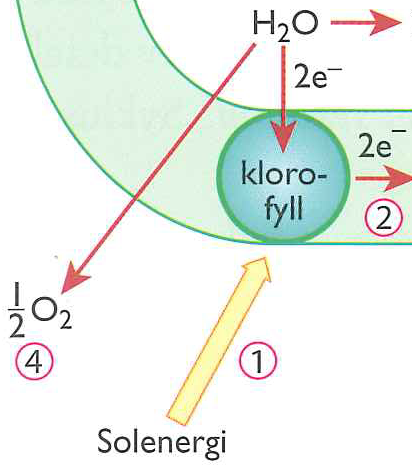
\includegraphics[width=0.4\textwidth]{img/data_analysis/light_dependent_detail.png}
\caption{Detail from the illustration of the light-dependent reaction \citep{bios}}
\label{fig:lightdependentdetail}
\end{figure}

\subsection{Misconception not followed up}

\subsubsection*{Context}
The teacher is standing in front of the group asking them questions to make them reflect on different aspects of the photosynthesis. The conversation follows a pattern where the teacher asks a question, and the students answer. As we enter the setting, Siri has just presented a hypothesis. As the teacher asks for other explanations, all of the students are looking down on the textbook illustration of the light-dependent reaction placed on the table in front of them (see figure \ref{fig:lightdependentdetail}). 

\subsubsection*{Excerpt 6}
\begin{table}[H]
	\begin{center}
		\begin{tabular}{r l p{7cm} p{3cm} } \toprule
			Time &  Who &  Speech  & Action \\ \midrule 
			12:34 %time
			&Lærer %name
			&\parbox[t]{7cm}{\raggedright ja det er et alternativ en alterna har dere noen andre eventuelle forklaringer? det kunne være andre forklaringer? %speech 
			}&\parbox[t]{3cm}{\raggedright  %action 
			}\\

			12:42 %time
			&Nora %name
			&\parbox[t]{7cm}{\raggedright kan jeg bar sp.. solener.. ehh kan det bare være lys også? %speech 
			}&\parbox[t]{3cm}{\raggedright Peker på ordet "solenergi" på modellen på arket %action 
			}\\

			12:45 %time
			&Lærer %name
			&\parbox[t]{7cm}{\raggedright Hva sier du %speech 
			}&\parbox[t]{3cm}{\raggedright bøyer seg frem for å høre bedre %action 
			}\\

			12:46 %time
			&Nora %name
			&\parbox[t]{7cm}{\raggedright Kan lys forårsake eksit.... at det eksiterer? eller bare sol? %speech 
			}&\parbox[t]{3cm}{\raggedright Tar fingeren langs pilen i modellen hvor det står "solenergi", og illustrerer at solenergi kommer inn til klorofyllmolekylene %action 
			}\\

			12:50 %time
			&Lærer %name
			&\parbox[t]{7cm}{\raggedright vanlig lys.. åja du mener lampe altså sånn grønt lys? %speech 
			}&\parbox[t]{3cm}{\raggedright  %action 
			}\\

			12:54 %time
			&Nora %name
			&\parbox[t]{7cm}{\raggedright mhm %speech 
			}&\parbox[t]{3cm}{\raggedright  %action 
			}\\

			12:55 %time
			&Lærer %name
			&\parbox[t]{7cm}{\raggedright Altså det er jo spørsmålet...  %speech 
			}&\parbox[t]{3cm}{\raggedright  %action 
			}\\

			12:57 %time
			&Nora %name
			&\parbox[t]{7cm}{\raggedright eller jeg mente ehh.. lys  %speech 
			}&\parbox[t]{3cm}{\raggedright peker opp mot lampene i taket %action 
			}\\
			12:57 %time
			&Siri %name
			&\parbox[t]{7cm}{\raggedright ... det var jo det de gjorde i skapet %speech 
			}&\parbox[t]{3cm}{\raggedright peker mot skapet %action 
			}\\

			12:58 %time
			&Lærer %name
			&\parbox[t]{7cm}{\raggedright Åja her inne? jammen få.. fikk de det inne i skapet? %speech 
			}&\parbox[t]{3cm}{\raggedright  %action 
			}\\

			13:00 %time
			&Nora %name
			&\parbox[t]{7cm}{\raggedright Nei jeg bare lurer jeg mm. %speech 
			}&\parbox[t]{3cm}{\raggedright  %action 
			}\\
		\end{tabular}
	\end{center}
	\caption{Misconception not followed up}
	\label{excerpt:misconceptionnotfollowed}
\end{table}

\subsubsection*{Analysis}
After the teacher has asked if there can be any other explanations, Nora takes the opportunity to ask the question: "...ehh can it be light as well?". As she asks the question, she points at the word "solar energy" in the illustration of the light-dependent reaction (see fig \ref{fig:lightdependentdetail} on page \pageref{fig:lightdependentdetail}). The teacher does not quite understand what she is asking, and therefore leans in and ask her to repeat the question. She reformulates her question in a more scientific language, asking if only sunlight can excite chlorophyll, and not artificial light. As she says the word "excite", she is pointing at the illustration of the chlorophyll molecule, and as she says "sun", she is pointing at the word "solar energy".

When Nora asks these questions, she refers to the illustration in front of her (as indicated by her pointing gesture). The reason for Nora asking is that in the illustration, photons are labeled as "solar energy" . This is probably done by the authors of the textbook to simplify the model as the audience is high school students, but in this case it leads to a big misconception. As we can see from her questions, she is unsure if artificial light can cause photosynthesis (which it can). If this were the case, Nora could rule out photosynthesis as the cause of the cabinet plant growing more than the window plant.

The teacher then proceeds to ask her if she means a lamp with green light, whereupon she confirms by saying "mmm". When the teacher replies that it is the question they are supposed to answer, she quickly replies that she meant artificial light, while pointing to the fluorescent ceiling lighting in the class room. The teacher then misinterprets her question, and think she is speaking of the specific lighting in the classroom, and not artificial light in general.

After Nora's question regarding the "erroneous" representation in the model, and the teacher's failure to understand the motivation behind the question, the discussion quickly takes another turn. The question is left hanging, it is not followed up later in the session.

\sout{Indicate that this will be followed up later?}


\section{Conceptualization}
\label{cha:conceptualization}

\subsection{Everyday language}

\subsubsection*{Context}
When we enter the setting, the teacher has just left the group. Morten has asked the students to look at the videos of the two different experiments and see if there are any differences in their appearance. The students have looked at plant B and found that it is mostly the stem that grows, not the leaves. Fredrik has requested that they should check plant A to compare the two, and Siri has just started the video from 29th of October, showing plant A. \sout{The group seems more motivated than in the next excerpt (\ref{excerpt:teacherintervention}), \textit{teacher intervention}.}


\subsubsection*{Excerpt 8}

\def\arraystretch{1.5}
\begin{table}[H]
	\begin{adjustwidth}{-4em}{-4em}
		\begin{center}
		\begin{tabular}{r l p{7cm} p{3cm} } \toprule
			Time &  Who &  Speech  & Action\\ \midrule  

			17:12 %time
			&Siri %name
			&\parbox[t]{7cm}{\raggedright Der åpner jo bladene seg med en gang nesten %speech 
			}&\parbox[t]{3cm}{\raggedright Nora ser mot planten på bordet %action 
			}\\

			17:15 %time
			&Fredrik %name
			&\parbox[t]{7cm}{\raggedright ja ... ((stillhet, venter til video er ferdig)) det kan jo ha noe med at her trenger den jo bladene for å ((tar hånden over bordet og beveger den raskt oppover som om han tar i mot noe)) \textbf{fange} lyset da, mens ((nikker mot skapet)) den trenger jo ikke det så mye inni skapet.. eh kanskje %speech 
			}&\parbox[t]{3cm}{\raggedright   %action 
			}\\

			17:34 %time
			&Siri %name
			&\parbox[t]{7cm}{\raggedright at den \textbf{bruker} næringen fra jorda og frøet mer i skapet? %speech 
			}&\parbox[t]{3cm}{\raggedright  %action 
			}\\

			17:37 %time
			&Fredrik %name
			&\parbox[t]{7cm}{\raggedright ehhhh.. ja. eller at den ikke utnytter den sol.. det \textbf{sollyset} inne i skapet så det den trenger jo ikke da også at bladene \textbf{spretter ut} så tidlig eller at... eh ja. %speech 
			}&\parbox[t]{3cm}{\raggedright  Gestikulerer med hånden som om den var planten som utnytter sol og vokser blader. %action 
			}\\

			\bottomrule
		\end{tabular}
		\end{center}
	\end{adjustwidth}
	\caption{Everyday language}
	\label{excerpt:everydaylanguage}
\end{table}

\subsubsection*{Analysis}
 First Siri mentions that the leaves are opening almost at once (compared to what they saw in the video from the cabinet). Fredrik approves, waits for the video to stop and then he says that plant A need leaves in order to "capture" light, while plant B does not need any leaves for that purpose. Siri asks if what he means is that plant B uses more food from the soil and the seed. Fredrik answers that plant B does not make use of the sunlight, hence it does not need leaves that "pops out" early. 

 The textbook Analysis of this phenomenon is that photosynthesis happens in the leaves. Photons become absorbed by different pigments that excite electrons, which again triggers the other parts of photosynthesis. Plants therefore need leaves in order to perform photosynthesis. Thus, the students are discussing a complex phenomenon using everyday language. Examples are (bold text in excerpt) \textit{capture} (fange) and \textit{use} (bruker) instead of \textit{absorb}, and \textit{sunlight} (sollyset) instead of \textit{photons}. 

\subsection{Teacher intervention}

\subsubsection*{Context}
The discussions preceding this excerpt has been a bit slow, leading us to intervene more in the situation, and asking more questions. The students still seem interested and concentrated, with Siri in the lead. The language used by the participants has up until this point been informal, and most utterances has been related to observations. A few seconds prior to excerpt 9 Sjur has instructed them to flip the task sheet, revealing an illustration from the textbook of the light-dependent reaction. INSERT FIGREF!!!

\subsubsection*{Excerpt 9}
\begin{table}[H]
	\begin{center}
		\begin{tabular}{r l p{7cm} p{3cm} } \toprule
			Time &  Who &  Speech  & Action \\ \midrule 
			11:20 %time
			&Lærer %name
			&\parbox[t]{7cm}{\raggedright Går det bra eller %speech 
			}&\parbox[t]{3cm}{\raggedright kommer bort til bordet og lener seg på det.%action 
			}\\

			11:23 %time
			&Siri %name
			&\parbox[t]{7cm}{\raggedright mmm, ja %speech 
			}&\parbox[t]{3cm}{\raggedright  alle nikker%action 
			}\\

			11:24 %time
			&Lærer %name
			&\parbox[t]{7cm}{\raggedright skjønner dere ... har dere funnet forklaring på alle spørsmålene? %speech 
			}&\parbox[t]{3cm}{\raggedright  %action 
			}\\

			11:26 %time
			&Alle jentene %name
			&\parbox[t]{7cm}{\raggedright *** vi prøver ... %speech 
			}&\parbox[t]{3cm}{\raggedright snakker i munnen på hverandre %action 
			}\\

			11:27 %time
			&Siri %name
			&\parbox[t]{7cm}{\raggedright Jeg tror kanskje jeg har en ide om det med at den her ute ((peker mot vinduet, refererer til planten i vinduet)) ikke vokser like høyt, eller så fort ihvertfall.. fordi atte når det kommer veldig mye sol så blir jo \textbf{klorofyllmolekylene eksitert}, men når alle ... alle \textbf{klorofyllene} blir \textbf{eksitert} i planten, sånn atte det ikke er flere som kan bli \textbf{eksitert} så hjelper det ikke om det er mere lys. %speech 
			}&\parbox[t]{3cm}{\raggedright  %action 
			}\\
		\end{tabular}
	\end{center}
	\caption{Teacher intervention}
	\label{excerpt:teacherintervention}
\end{table}

\subsubsection*{Analysis}
When the teacher approaches the group, Siri's language quickly change from explaining things in everyday terms to a more precise scientific language. After roughly 11 minutes of discussion, first occurrences of the words like \textit{excited}, \textit{chlorophyll}, and \textit{molecules} (bold text in excerpt) appear. 

One reason for the sudden change in language may be that only seconds before the excerpt, the students looked at the figure from the textbook, representing the light-dependent part of photosynthesis \sout{SEE FIGREF INSERT HERE}. This may have led Siri onto a more theoretical path of explanations, causing her to try and explain the phenomenon using scientific language. 

Another explanation of this phenomenon may be that when the teacher asks a question, the students think he will be assessing the answer. Thereby creating a test-like situation for the students, where Siri is eager to express her knowledge about the photosynthesis model as explained in the textbook. 

\sout{will be followed up as institutional stuff in discussion}

\subsection{Scientific language}
\subsubsection*{Context}
The students work with task 3 regarding soil moisture and differences in absorption rate. Most of the discussions have been concerned with making general observations, and they are struggling to form new hypotheses. The main observation is that there are major differences in the absorption rate in the two experiments. In an effort to push the discussion further, Sjur (researcher) has started to intervene, asking what it could mean in terms of photosynthesis that the soil moisture level drops less in the end of the experiment (see Figure \ref{fig:soilmoistscreenshot}). Approximately one minute before excerpt 10 starts, the teacher has tried to position himself discretely behind the group, but all the students except Linda has noticed him. As we enter the setting, Nora initiates the discussion.

\subsubsection*{Excerpt 10}
\begin{table}[H]
	\begin{center}
		\begin{tabular}{r l p{7cm} p{3cm} } \toprule
			Time &  Who &  Speech  & Action \\ \midrule 
			29:16:00 %time
			&Nora %name
			&\parbox[t]{7cm}{\raggedright men det er sånn...fordi vi har jo...det er jo den \textbf{lysuavhengige} delen av \textbf{fotosyntesen} også...jeg vet ikke om den har...\textbf{atp} og \textbf{nadph} fra f... %speech 
			}&\parbox[t]{3cm}{\raggedright ser mot Sjur mens hun snakker, vender seg mot Fredrik når han avbryter henne %action 
			}\\

			29:26:00 %time
			&Fredrik %name
			&\parbox[t]{7cm}{\raggedright ...den må jo ha den...først drive den lys... eller den må jo drive den \textbf{lysavhengige} også for å drive den \textbf{lysuavhengige} %speech 
			}&\parbox[t]{3cm}{\raggedright bruker hendene til å vise at den lysuavhengige reaksjonen er avhengig av den lysavhengige reaksjonen %action 
			}\\

			29:35:00 %time
			&Siri %name
			&\parbox[t]{7cm}{\raggedright mhm %speech 
			}&\parbox[t]{3cm}{\raggedright  %action 
			}\\

			29:36:00 %time
			&Fredrik %name
			&\parbox[t]{7cm}{\raggedright ...den har vel ikke \underline{atp} eller \underline{nadph} fra før av? %speech 
			}&\parbox[t]{3cm}{\raggedright alle ler %action 
			}\\

			29:44:00 %time
			&Nora %name
			&\parbox[t]{7cm}{\raggedright ja det var det jeg lurte på også %speech 
			}&\parbox[t]{3cm}{\raggedright  %action 
			}\\

			29:46:00 %time
			&Siri %name
			&\parbox[t]{7cm}{\raggedright nei det er vel den \textbf{lysavhengige} reaksjonen bruker til å danne det? %speech 
			}&\parbox[t]{3cm}{\raggedright  %action 
			}\\
		\end{tabular}
	\end{center}
	\caption{Scientific language}
	\label{excerpt:scientificlanguage}
\end{table}

\subsubsection*{Analysis}
After failed attempts to explain the observation of difference in absorption rate in the two experiments, Nora suddenly switches to a more scientific language than in the minutes preceding this discussion. The words emphasized in bold can be found both in the textbook and in the language used by the teacher in earlier presentations of the material. 

There may be several reasons for this sudden change in language. \emph{First}: Sjur has asked an intervening question, and while she is answering this, she is looking at him as if he knows the answer, leading to a test-like situation. \emph{Second}: the teacher is standing behind her listening to the whole situation. \emph{Or third}: she is simply trying to bring in another representation as the students have not yet been able to explain the phenomena with the use the physical plant and the system. 


\section{Linking representations}
\label{cha:linking}
\subsection{Soil moisture representation}


\subsubsection*{Context}
The students have read the introduction to assignment 3: \emph{"Look at the soil moisture graph for the whole period of the experiment. Plant A was sown on 25th of October and plant B was sown 1st of November."} Siri has navigated to the soil moisture graph in the system (see Figure~\ref{fig:soilmoistscreenshot}), and got some help from Sjur to navigate the graph. Siri expanded the graph to include the lifespan of both plants and Sjur explained that this was indeed what they were looking at. Siri lets go of the mouse and keyboard to read assignment 3a: \emph{Is there any difference in the absorption rate?} It is at this point we enter excerpt 11



\subsubsection*{Excerpt 11}

\def\arraystretch{1.5}
\begin{table}[H]
	\begin{adjustwidth}{-4em}{-4em}
		\begin{center}
		\begin{tabular}{r l p{7cm} p{3cm} } \toprule
			Time &  Who &  Speech  & Action\\ \midrule  

			21:34 %time
			&Nora %name
			&\parbox[t]{7cm}{\raggedright Åja, fra de... den og den ((peker på høyre og venstre side av grafen)) %speech 
			}&\parbox[t]{3cm}{\raggedright Lager v-tegn med fingrene og viser hvilken periode i grafen planten var i vinduet, og hvilken periode den var i skapet %action 
			}\\

			21:36 %time
			&Sjur %name
			&\parbox[t]{7cm}{\raggedright ja. %speech 
			}&\parbox[t]{3cm}{\raggedright  %action 
			}\\

			21:37 %time
			&Siri %name
			&\parbox[t]{7cm}{\raggedright Åja, så det der er den ene planten og det der er den andre.. %speech 
			}&\parbox[t]{3cm}{\raggedright Peker først på venstre side av grafen, så på høyre %action 
			}\\

			21:41 %time
			&Nora %name
			&\parbox[t]{7cm}{\raggedright mhm, den der går litt brattere ned på ... %speech 
			}&\parbox[t]{3cm}{\raggedright Peker på området i grafen hvor planten sto i skapet %action 
			}\\

			21:44 %time
			&Fredrik %name
			&\parbox[t]{7cm}{\raggedright Ja, den går mye brattere ned. %speech 
			}&\parbox[t]{3cm}{\raggedright  %action 
			}\\

			21:46 %time
			&Siri %name
			&\parbox[t]{7cm}{\raggedright Kanskje det betyr at den der andre planten bruker mye mer fuktighet fra jorden %speech 
			}&\parbox[t]{3cm}{\raggedright Peker på området i grafen hvor planten sto i skapet %action 
			}\\

			\bottomrule
		\end{tabular}
		\end{center}
	\end{adjustwidth}
	\caption{Linking between representations}
	\label{excerpt:soilmoistureexcerpt}
\end{table}

\begin{figure}
	\centering
	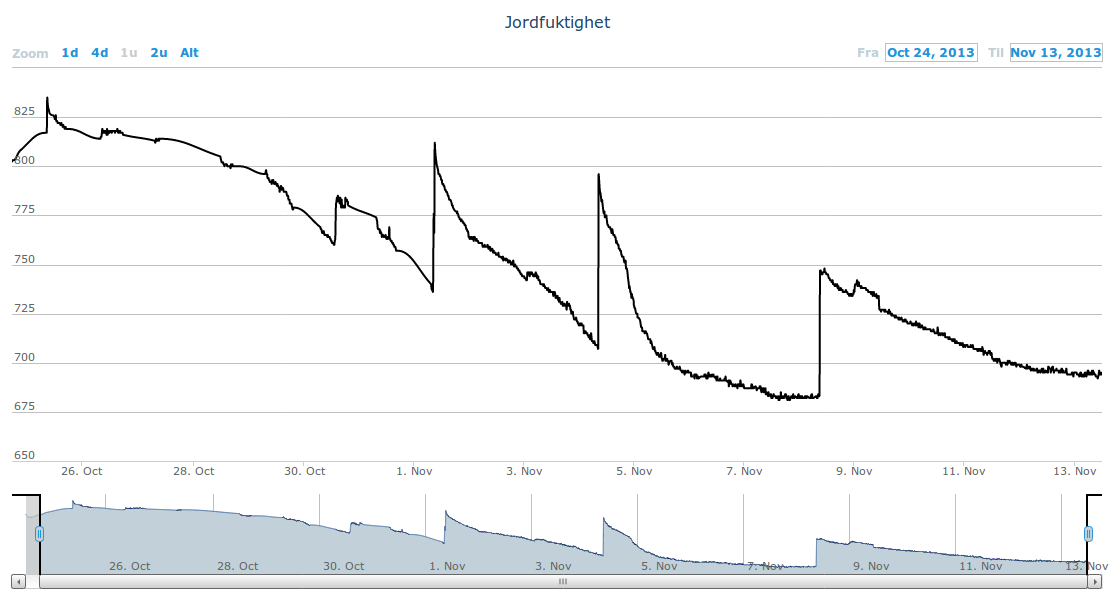
\includegraphics[width=1.0\textwidth]{img/dataandanalasys/soilmoisturegraph.png}
	\caption{Screenshot from the soil moisture graph}
	\label{fig:soilmoistscreenshot}
\end{figure}

\subsubsection*{Analysis}
Here the students are looking at Monoplant's representation of the soil moisture over time (see figure~\ref{fig:soilmoistscreenshot}). At first they try to interpret what part of the graph is which plant. First, Nora shows by pointing with a V-shaped hand which part of the graph that represents plant A and plant B. Siri follows up and explains in an acknowledging way by pointing first to the left and then to the right. When this is confirmed and the students understand how the graph is divided between the two experiments, they start to interpret what the graph tells them. Nora observes and tell the others that the curves from the plant in the cabinet is much steeper than from the one in the window. The other students agree and Siri claims that the plant in the cabinet uses a lot more water. Hence it seems like the students are interpreting the graph to represent the water ($\text{H}_2\text{O}$) usage of the plant. 

This might be for several reasons. For example the textbook shows that plants use $\text{H}_2\text{O}$ in both the light dependent and the light independent reactions, so the students knows that $\text{H}_2\text{O}$ plays a central role in photosynthesis. There are also some constraints for interpretation in the system. First it is designed to represent a plant, hence it would be hard to interpret the soil moisture graph to not represent the life of the plant. Lastly there is the assignment: \emph{"Is there any difference in the \textbf{absorption} rate?"} By using the word absorption, we have constrained the interpretation of the graph, which lead the students to focus on the plants absorption of $\text{H}_2\text{O}$.

 %!TEX root = ../document.tex
\chapter{Discussion}
In this chapter we will discuss our research question by contextualizing our findings to the theoretical concepts introduced earlier . As an overall theme we will look at the inquiry process of the students in interaction with Monoplant. This will be showed through 4 sections, the first being about the inquiry process. Next we will discuss how multiple external representations support the inquiry process of the students, then how scaffolding is instantiated in the environment, and finally how the institutional setting frame the students' inquiry process.


\section{Inquiry process}
In this section we will broadly address our first research question: \emph{"What characterizes the students’ inquiry in interaction with monoplant?"}
In the previous chapter we presented excerpts from the session where the students interacted with monoplant. We have seen that the students were generating hypotheses of what happened with the plant and why it grew as much as it did. We showed examples of explanations, discussion, misconceptions and surprises.

\subsection{Tentative hypothesis}
We designed the experiments together with the teacher. The students were given a problem in form of the assignments they discussed but needed to figure out the answers by themselves with the help of Monoplant, which presented detailed data logging of the experiments. The experiments conducted combined with the problem solving-session with the students can be categorized as \emph{guided inquiry}  \citetext{\citet{staver1987analysis}, referenced in \citealp{prince2006inductive}}. 

As showed in excerpt 1, Siri presented a hypothesis in which she stated that plant B would not grow much because it would not get as much light as plant A. In excerpt 2 data was presented to her that showed that plant B had indeed grown much. Her interpretation of this data was directed by her first hypothesis and because the data disconfirmed it, the next hypothesis is claiming there might be some error source in the experiment. Hence the misinterpretation did not result in a direct confirmation of the previous hypothesis, instead it laid the basis for a denial of a disconfirmation, or an explanation for why the first hypothesis did not hold even though she still thinks it should.

The four problems that \citet{de1998scientific} addressed for inquiry learning where: \textit{hypothesis generation}, \textit{design of experiments}, \textit{interpretation of data}, and \textit{regulation of discovery learning}. In our case we controlled two of these problems by designing and initiating the experiments for the students, as well as letting Monoplant do a systematic logging of data during the experiment, hence regulating the inquiry process. This meant that the students faced two problems, interpreting the data and generating hypotheses based on the data. \citeauthor*{klahr1993heuristics} \citetext{\citeyear{klahr1993heuristics}, referenced in \citealp{de1998scientific}} reported that misinterpretation of data often result in confirmation of current hypothesis. 



\subsubsection*{Delay inquiry}
As the students were done with the textbook chapter of photosynthesis and were able to explain  phenomena such as growth theoretically, the presumptions of the outcomes to the experiment colored the interpretation of data because it was connected to the student's prior conceptual knowledge. Siri knew that plants make food for themselves by doing photosynthesis. To do photosynthesis, a green plant such as the cress in the experiment needs light of wavelengths other than green (blue and red). This reasoning makes sense to Siri because she knows a lot of the scientific concepts concerning the theme at hand. We can say that the inquiry process became deductive as it was affected by the students preconceptions and their ability to explain the observations they made with Monoplant. 

However, this is a misconception in inquiry learning, and what \citet{gomez2008elementary} refers to as inconsistent understanding, according to what the teacher intended. In this case Siri's conception of photosynthesis, which in the context of the textbook examples makes sense, becomes a misconception when she is confronted with a plant that germinates. Hence it leads her to an erroneous conclusion. \citet{smith1994misconceptions} makes the description of this kind of misconceptions as "faulty extensions of productive prior knowledge". So that a conception might help describe a phenomenon in one context, but falsely describe it in another context. \citeauthor{klahr1993heuristics} sets words to what seems to be the main issue: 

\begin{quote}"compared to the binary feedback provided to subjects in the typical psychology experiment, real-world evidence evaluation is not so straightforward" \citetext{\citet[p. 114]{klahr1993heuristics}, referenced in \citealp{de1998scientific}}
\end{quote}

Even though our field of study is different from \citeauthor{klahr1993heuristics}, this distiction helps us to illustrate what we can see in the students inquiry: the context of the plant in the experiment is new for the students, making it difficult for them to apply their prior knowledge to the phenomenon. 

We have now established that the inquiry process is influenced by the fact that the students have certain knowledge about photosynthesis. Coming into the experiment, this can at one hand lead to misconceptions due to the students having a great freedom to pursue their ideas through the inquiry process. In that case, these misconceptions should be followed up and corrected. On the other hand, the system or an instructor or can guide the students to pursue the fruitful ideas from the start, staying one step ahead of possible misconceptions. We will discuss this further in the section about scaffolding.



\section{Multiple External Representations in Inquiry processes}
During the inquiry process the students were presented with different representations of the photosynthesis phenomenon. In this section we will give account for how those representations were used in the inquiry process and how they complimented each other. We will also look at differences in the students' language when engaging in talk with the different representations. To recap, our second research question is as follows: \emph{"How does Monoplant, by presenting photosynthesis differently from the text book, support the inquiry process?"}

\subsection{Complementary processes}
%How does textbook present photosynthesis
When reviewing the textbook used in science education, we found that the scientific concepts are largely represented in a theoretical manner. In the first paragraph of the chapter concerning photosynthesis, scientific words such as "pigments", "chloroplasts" and "glucose" appear. Later on, photosynthesis is explained by its chemical formula and the chapter rarely gives any examples of how photosynthesis affects the life of plants concretely. The textbook therefore emphasizes how photosynthesis fits into a larger system of scientific concepts, and is more concerned with conveying the big picture than the specific and concrete experiences. 

%How does monoplant represent photosynthesis
Monoplant on the other hand affords a more inductive or "bottom-up" approach. As a learning resource, Monoplant is a tool for exploring ideas related to photosynthesis. The variables relevant for the plant's photosynthesis are mediated through graphs and videos, but leaving the interpretation of these data in the hands of the students. The system is only concerned with one plant in one specific context, and not trying to generalize from the specific results to a larger scientific concept. 

When looking at our data with this in mind, a pattern in the students' language emerge. During the inquiry process, students use everyday language when engaging with Monoplant. An example comes from excerpt 10 where Siri says that the plant "use moisture from the earth". Another example is from excerpt 7 where students use concepts as "pop out", "capture" and "use sunlight". All of these concepts have their scientific counterpart that is represented in the textbook, but when discussing among themselves, the students choose to talk about the phenomenon in a "non-academic" way. 

However, the students' language seem to change when engaging with representations linked to the textbook. An example of this is from excerpt 8 where Siri use scientific concepts such as "chlorophyll molecule" and "excited" when looking at a textbook illustration of photosynthesis. 

An explanation of the change in language may be given by applying \citet{vygotsky2012thought} theory of spontaneous and scientific concepts as presented in chapter \ref{cha:spontaneous_scientific} on page \pageref{cha:spontaneous_scientific}. When engaging with Monoplant, the students are addressing concrete results in a concrete experiment in a specific context. The concepts they use are therefore linked to what they are observing. When Siri says that the plant "use sunlight", it is because this is something he has experience with. She knows that the sun transfers energy that plants make use of, and she has perhaps seen plants die as a result of receiving no light. This is an example of a spontaneous concept \citep{vygotsky2012thought} - "a nonconscious and nonsystematic" concept. Spontaneous concepts have their strength in explaining what concerns the situation, empirical and practical \citep{vygotsky2012thought}, and are therefore deemed fit to mediate the student's thoughts when discussing the plant on the screen in front of them. 

%The corresponding scientific concept in this case would be to "excite electrons", but this is an abstract concept that is difficult to link any concrete experiences to. As a result she feels more comfortable using the spontaneous concept: to "use sunlight" when explaining her thoughts to the other students. 

Yet we see from excerpt 8 that the same student also use the scientific concept "excite electrons" when describing the same phenomenon but interacting with the textbook instead of Monoplant. This is a more abstract concept, but has its strength in its "conscious and deliberate character" \citep{vygotsky2012thought}. An explanation of the change in language may be that the student is not aware of the two concepts referring to the same phenomenon. She masters the scientific concept only in the realm of the textbook and the concept's relation to other scientific concepts. And she masters the spontaneous concept only when referring to the concrete experiments where they have observable results. 

Another more plausible explanation would be that in engaging with both Monoplant and the textbook she has mastered both the scientific and spontaneous concept of exciting electrons. The spontaneous concept has "in it's slow way upwards cleared the path for a scientific concept" \citep{vygotsky2012thought}. The student is therefore able to speak of "exciting electrons" both when talking about the concrete experiment, and when discussing the experiment in more abstract terms. 

Vygotsky states that the "development of scientific concepts runs ahead of the development of spontaneous concepts". The school has therefore in this setting supplied the curriculum necessary for the scientific concept generation. Whereas the students' inquiry process with Monoplant has supplied a framework for enriching the scientific concept with personal experiences.

On the other hand, we do not find any evidence of the other participants mastering the concept of "exciting electrons" on the same level as Siri. Yet they are able to discuss the matter with her using the spontaneous concept. This would suggest that the other students are not far away from mastering both the scientific and spontaneous concept. In line with \citet{vygotsky2012thought} we will argue that the control the spontaneous concepts lacks lie within the Zone of Proximal Development for the other students. 

We believe our data warrants the assumption that different types of representations spurs complementary processes that can lead to stronger concept comprehension among the students. Inquiry-based environments have their strength in that they provide personal experiences, while more scientific representations are able to place the phenomenon in a broader scientific context. As scientific concepts and spontaneous concepts mutually enrich and are dependent on each other \citep{vygotsky2012thought}. It is important to take the development of both into account when designing learning environments. 
%As shown, using Monoplant in the inquiry process can provide concrete experiences which helps the concept "come to life" \citep{van1998concept}. 
%Can we write about inquiry learning in general as spontaneous concepts? Can this be elaborated?




\subsection{Complementary roles}
During the inquiry process the students were faced with three fundamentally different representations of the same phenomenon: the textbook, the physical plant, and the digital Monoplant system. The textbook consists of textual representations, along with pictures, illustrations and graphs. The physical plant is a real-life representation of photosynthesis in action. And the Monoplant system mediates information such as timelapse-videos that would otherwise be unavailable in the real world. 

As pointed out by \citet{van2006supporting} there are many benefits of representing the same phenomenon in multiple ways. First, each of the representations can show specific aspects of the domain to be learned. Second, one representation can constrain the interpretation of another representation. And third, learners can build abstractions by translating between the representations, which may lead to a deeper understanding of the domain. In our case Monoplant was used to convey external factors' effect on photosynthesis. Using both qualitative information in the form of videos and the physical plant, and quantitative in the form of graphs. 

But while the benefits of using MER in education seem obvious, both \citet{ainsworth1999functions} and \citet{van2006supporting} point to problems students face while undergoing extra tasks related to MER. To exemplify, let us first take a look at the different representations within the Monoplant system. The first task the students then have to face is to understand the syntax of the representations. E.g. one of the graphs represented is relative, meaning that the different units of measurement of the sensorvalues are discarded and replaced with percentage-values. The students then have to understand what the different axes of the graph represent and how the variables relate to one another. Second, the students have to understand which parts of the domain are represented. The system is designed in such a way that it does not constrain to one specific form of interaction, and the relation between Monoplant and external factors' effect on photosynthesis can therefore be somewhat obscure. And finally, the students have to understand the relation between the different representations. E.g. when playing a video file, it is necessary to see it in relation with the graph to get both the quantitative and qualitative aspects of the phenomenon. 

In our data we see evidence of the students having problems with the latter of these tasks: comprehending the relation between the different representations. 




\subsection{Representation becomes Misconception}
As mentioned earlier, explanations can be accurate enough for one situation but lead to false conclusions in other situations. \citep{smith1994misconceptions} This is true for representations and models as well and becomes evident if we look at Excerpt 6. After looking at the textbook representation that uses the word "solar energy" to label photons, Nora asks "Can light cause excit.. that it excites. Or is it just the sun?". As the book provides the context to photosynthesis it mostly frames examples to the nature where sunlight and solar energy is indeed valid simplifications of photons. But in the case of the experiments with Monoplant, this simplification is challenged but not addressed. Monoplant show how much light the plant got, but does not distinguish what sort of light. The experiments were however designed in such a way that it differentiated light quality (wavelength of light). Nora might have interpreted the experiments to address differences to a plant that have access to solar energy and one which gets another type of light energy. In any case this is a good example of how an explanation can be plausible and have explanatory power in one setting, but lead to erroneous conclusions in another setting. This is also a great example of the need for scaffolding in an inquiry process, which leads us to the next section........ . . . 









How does Monoplant, by visualizing/present photosynthesis differently from the text book, support the inquiry process? 
Here we can talk about: 
\begin{itemize}
\item{how do the textbook represent photosynthesis/external factors}
\item{how do Monoplant represent photosynthesis/external factors}
\item{\nameref{ex:excerpt10} (soilmoist)}
\item{\nameref{ex:excerpt6} (misconception from textbook representation)}
\item{Excerpts: 2, 3, 4, 6, 7, 8, 10}
\item{MER}
\item{Social practices}
\item{Everyday language \& Scientific language}
\end{itemize}




\section{Scaffolding}
How is scaffolding instantiated in the environment?
Here we can talk about: 
\begin{itemize}
\item{ZPD}
\item{Scaffolding}
\item{Inquiry learning}
\item{Misconceptions}
\item{Excerpts: (3), 4, 5, 6, 8, 9}
\end{itemize}



\section{Institutional setting}
How does the institutional setting frame the students inquiry process? (“doing school \& doing science”)
By this we mean to set focus on how the institutional setting affects the students interaction with monoplant and their inquiry process. 
embedded stuff: datalogging, -assignments, language,
Filming and records the session made it possible for the students to keep an oral discussion without actually writing any answers down on paper. 

students using knowledge, brilliere med kunnskap for å vise kontroll på pensum.

\begin{itemize}
\item{Institutional settings}
\item{Inquiry learning}
\item{Everyday language \& Scientific language}
\item{Excerpts: 1, 5, 8, 9}
\end{itemize}

=======
%!TEX root = ../document.tex
\setcounter{page}{1}
\pagenumbering{arabic}
\chapter{Introduction}
In this master thesis we will look at how students use a plant monitoring system called Monoplant to support their scientific inquiry when learning about photosynthesis. 

%Computer based technology are increasingly being used for educational purposes, both in school settings and student-initiated settings. As of 2009 every high school student in Norway should have a personal computer available for use (UDIR). The use of ICT is receiving increased attention as it is believed that it can enhance students learning and provide productive learning environments. One important point is that the usage of ICT is important in itself to prepare students for working with technology. However, making use of the opportunities these technologies give us, by applying digital content specifically designed for educational contexts, is in our opinion of equal importance. 

With the advent of Internet-connected embedded devices, we face an opportunity to distribute time consuming and tedious tasks to computers. By using digital sensors, one can initiate the collection of quantitative data from our surroundings and do other things while a computer handles monotonous tasks such as logging and storing of the data. Say we want to conduct an experiment where we log the temperature throughout a day. Instead of walking over to the thermometer every 15 minutes to write down the temperature, a computer can read and store the temperature in a database. This technology has been used by meteorologists, scientists and commercial operators for a long time, but the technology is now becoming so cheap that regular people can afford it. %An important positive effect of this is of course that we can save a lot of time when gathering quantitative data, but we think a more interesting aspect is what can be done with this data. 

A popular uprising usage is automation of tasks, as one can make the computer react to the data based on some preset thresholds regarding the values. There is for example automated watering systems that water plants based on readings of the soil moisture, or heating systems that turn on if the temperature is below a value. Automation can indeed take loads of work off our backs and thereby save us time. While there is truly a market for this, we think an even more interesting usage of such data exists and it consists of interpretation. The logged data can be accessed and presented in any way we want. This creates a great possibility for creating digital content from the real world and design it to be used in educational contexts.


\section{Motivations and background}
When we started working with ideas for this thesis, our goal was to do research on an actual product in a real world setting. As we chose to develop a system ourselves, a major part of the work on this thesis became to build and complete the system. In 2012 during a project in inf5261 - \emph{Development of mobile information systems} we developed a mixed reality game called Plantagotchi. The prototype developed in this course became the foundation of the system in this thesis referred to as Monoplant. The idea was to animate a digital version of a real plant, which was affected by how the real plant was treated. In this project the user group was children at the age of 8-12 and the game was planned to be used as a school contest where classes competed in getting the happiest plant. The educational outcome being pupil motivation for learning about growth conditions for plants, so that they could win the game. 

\begin{figure}
\centering
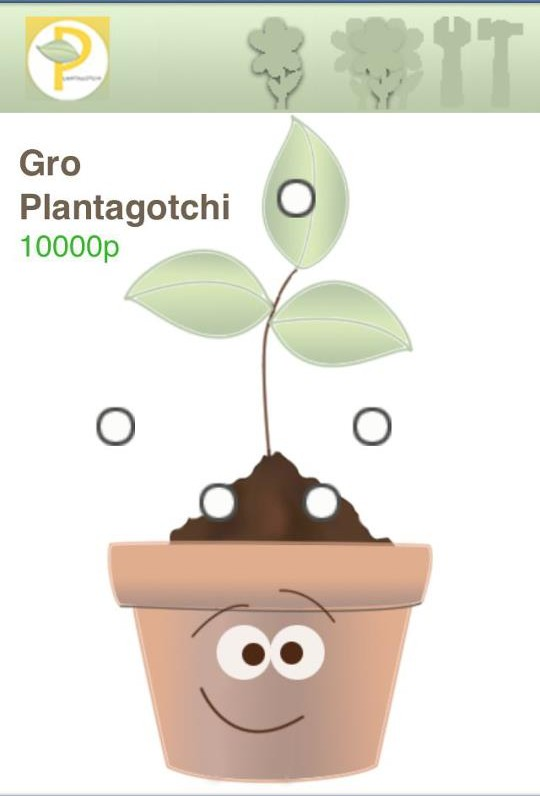
\includegraphics[width=0.5\textwidth]{img/introduction/plantagotchi.jpg}
\caption{Screenshot of Plantagotchi prototype}
\label{fig:scrshotplantagotchi}
\end{figure}

During the spring of 2013 we both took the course inf5790 \emph{Technology enhanced learning} and were introduced to the field of Computer Supported Collaborative Learning (CSCL). As we brought with us an idea of an application that pupils could use to collaboratively learn about a scientific domain, CSCL became the field where we could adapt theoretical perspectives and concepts, which set words to and explained our personal ideas and experiences. 

As mentioned, the starting point of this thesis was to do research on an actual working system, in an authentic environment. We therefore brought with us the ground idea from Plantagotchi and spent a lot of time improving it and developing a new working prototype. Furthermore, in October 2013 we got in touch with a school, and had a fully working plant monitoring system which we could test with real users in their natural setting. The focus in this thesis is therefore directed to this design experiment study performed in a high school biology class. We will however provide some background information about the decisions made while developing Monoplant. 


\section{Monoplant}
Plants live a slow life, they grow slowly and move slowly. Humans have no means of directly observe when a plant grow, but we are able to see that it has grown or bloomed. However, humans have the ability to use tools in order to make sense of the world, and we have created such a tool: Monoplant, which can help us see how plants evolve over time.

Monoplant is a monitoring system for plants, or rather humans who want to monitor their plants. It continuously gathers data about a plant's environment and makes the data available to the users via the Internet. One functionality is thereby to remotely monitor a plant and get instant data about temperature, humidity, light-level, soil moisture and even a picture of the plant. However, one of the main reasons for designing Monoplant, was that we wanted to see how plants develop over time, or in biological terms their ontogenetic development. Hence we tried to combine readings over time to see if we were able to observe if some of the variables affected the plant physically. The first step became to merge the images taken into a time-lapse video. This made it possible to see a plant's physical development throughout a day in a matter of seconds. In order to link this with the variables from the environment, we had to connect each image in the video to it's corresponding data reading. This is done by presenting a graph together with the time-lapse video and marking the point in the graph which corresponds to the current image in the video (see figure~\ref{fig:scrshotgraphlapse}). Thus we are connecting \emph{visible} changes of the plant (i.e., the video) to \emph{invisible} changes in the environment (e.g., soil moisture and humidity levels).


\begin{figure}
	\centering
	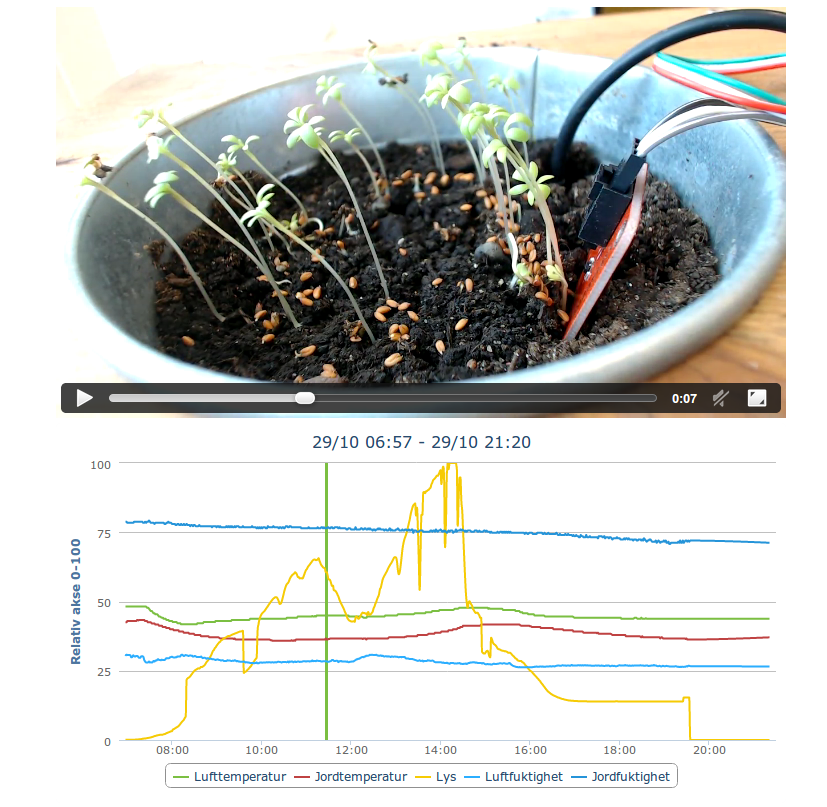
\includegraphics[width=\textwidth]{img/introduction/graphlapse.png}
	\caption{Screenshot of timelapse and graph}
	\label{fig:scrshotgraphlapse}
\end{figure}

%Maybe write something about how this is generic, but that in this thesis we have chosen to focus on how it can be used in learning.

\section{Research questions}
%place our focus in the CSCL field
As mentioned, the overall theme of this thesis will be how students can use Monoplant in their scientific inquiry when learning about photosynthesis in a biology class. This will be investigated through an analysis of a study performed the autumn of 2013. In order to address this broad theme we will try to answer four research questions. The first question is: 


\begin{noindlist}
\item \emph{"What characterizes the students’ inquiry in interaction with Monoplant?"}\\
This will naturally adress the characteristics of the students' actions and interactions during their work with Monoplant. The first question will also be elaborated through the next three questions.
\item \emph{"How does Monoplant, by presenting photosynthesis differently from the text book, support the inquiry process?"}\\
This question is indicating that there is a difference between the representation of photosynthesis in the school textbook and in Monoplant. To answer this we will address these differences, and discuss what implications they have in the students' inquiry process.
\item \emph{"In what way is scaffolding operationalized in the environment?"}\\
For this question to make sense, we need to introduce the theoretical concept of \emph{scaffolding} and put it in a broader context of instructional theory. This will be elaborated later in the thesis, but for now we can call it training wheels. We will look at how the teacher and Monoplant help the students in their inquiry process.
\item \emph{"How does the institutional setting frame the students inquiry process?"}.\\
As the study took place in a school setting, we wanted to look at how the social practices within school affected the inquiry process.
\end{noindlist}


\section{Thesis outline}
%scientific backgroud 
%technical background
%theory
%empirical & method
%data and analysis
%discussion
%concluding remarks
We will now present an outline for this thesis, providing an overview of the content as well as the structure. 

\subsubsection*{Chapter 1 - Introduction}
The introduction presents our personal and professional motivations for writing this thesis, a brief introductions to Monoplant followed by the research questions, and lastly this "readers guide".

\subsubsection*{Chapter 2 - Scientific background}
This chapter is an introduction to photosynthesis and thereby the scientific language within the domain. The introduction represents what the students in our case are supposed to learn in \emph{Biology 2}. It is provided as a tool to understand what we mean later in the thesis when using domain specific terms such as \emph{"light dependent reaction"}, \emph{"excited"} or \emph{"chlorophyll molecules"}.

\subsubsection*{Chapter 3 - Technical architecture and programming}
%The application is divided into three logical units: data collection, data processing and database, and user interface. In the following sections these units will be explained further. 
A major part of the work done was to design and build Monoplant. In this chapter we will describe Monoplant's architecture and address some of the technical concerns we met during the development process. We will introduce \emph{Raspberry Pi}, \emph{Arduino}, \emph{Ruby on Rails}, \emph{REST} and other frameworks and tools used to build Monoplant.

\subsubsection*{Chapter 4 - Theoretical perspective and concepts for analysis}
%In this chapter we will lay forth the theoretical perspective and theoretical concepts we will apply in this thesis. First we will introduce the \emph{sociocultural perspective} and highlight some key points including \emph{institutional practices}, \emph{zone of proximal development} and \emph{scaffolding}. Further we will look at \emph{multiple external representations} and lastly the concept and method of \emph{Inquiry learning}.

In this chapter we will present the sociocultural perspective, which will be used throughout this thesis. We will also introduce the theoretical concepts: \emph{spontanous and scientific concepts}, \emph{zone of proximal developement (ZPD)}, \emph{scaffolding}, \emph{multiple external representations (MER)}, \emph{institutional settings}, \emph{inquiry learning} and \emph{misconceptions}. We will make an account for our interpretation of these concepts as we will use them later in the thesis to help answer our research questions. 

\subsubsection*{Chapter 5 - Empirical setting and method}
%In this chapter, we will present the empirical setting and methods used in this thesis. First we will describe the empirical setting in which the data collection took place. Then we will proceed to present the methods for gathering data with a description of the technicalities of the data. Lastly, we will describe the procedures for selection and analysis of data.

Throughout October 2013 we gathered data for this thesis. In this chapter we will introduce \emph{design based research} and describe the empirical setting in which this data gathering took place. We will also describe the methods used for collecting the data and how we chose to use those methods. Lastly we will explain how we approached, selected and made sense of the data once the data collection was done. 

\subsubsection*{Chapter 6 - Data and analysis}
%In this chapter we will present the findings from our case study with a focus on themes relevant to our research questions. Each of the themes contain at least one excerpt with a context description, excerpt from the transcript, and an analysis of the unfolding events.
Here we will present the main findings from our study. The chapter contains 10 data extracts, which is presented one by one. First by a context description, then a data transcript and finally a clarification and analysis of what happened. 

\subsubsection*{Chapter 7 - Discussion}
%In this chapter we discuss our research questions by contextualizing our findings according to the theoretical concepts introduced earlier. As an overall theme we look at the inquiry process of the students in interaction with Monoplant. This will be showed through 4 sections, the first being about the inquiry process itself. Next we will discuss how multiple external representations support the inquiry process of the students. Then how scaffolding is instantiated in the environment, and finally how the institutional setting frame the students' inquiry process.
In this chapter we will discuss our research questions by applying the theoretical concepts introduced in chapter 4. Our first research question \emph{"What characterizes the students’ inquiry in interaction with Monoplant?"} will be the overall theme of this chapter, but all four of the questions will be addressed.

\subsubsection*{Chapter 8 - Concluding remarks}
Our concluding remarks will provide the reader with an overview of how we approached this thesis and a review of our main findings according to the research questions. Lastly we will present shortcomings and suggestions for further work.
%!TEX root = ../document.tex
\chapter{Scientific background}
\label{cha:scientificbg}
In this chapter we will first give a rudimentary introduction to photosynthesis as it is described in the curriculum for Biology 2 \citep{bios}. Then proceed to some monitoring and automated systems, which will lead to the next chapter, an introduction to Monoplant and its technical specifications.

\section{Photosynthesis}
The variables that we monitor in our application are directly linked to the precondition of all life, photosynthesis. During this process plants transform energy from light to chemical energy in the form of e.g., glucose and starch. As most organisms are not able to make use of light energy directly, plants are a necessity for producing energy that other organisms can transform. The equation for photosynthesis is written as: \ce{(CO2)n + (H2O)n + photons -> (CH2O)n + (O2)n}, which means that carbon dioxide, water and light transform to glucose and oxygen.  

Photosynthesis consists of two main parts: the light-dependent reaction, and the light-independent reaction. The light-dependent reaction, as the name implies, occur only in the light. The light-independent reaction occurs both in the light and dark, but does not rely on energy from photons.  

\begin{figure}
\centering
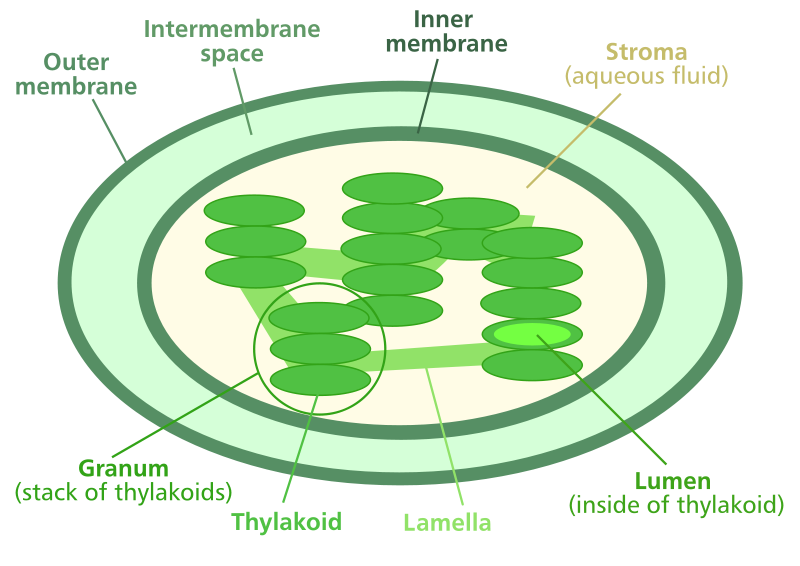
\includegraphics[width=0.8\textwidth]{img/photosynthesis/Chloroplast_diagram.png}
\caption{Illustration of a chloroplast molecule \citep{wiki:chloroplast}}
\label{fig:chloroplast}
\end{figure}

\subsection{Light-dependent reaction}
The light-dependent reaction consists of two different photosystems (photosystem 1 and photosystem 2) creating adenosine triphosphate (ATP) and nicotinamide adenine dinucleotide phosphate (NADPH) molecules for the light-independent reactions. Both systems are located in the thylakoid membrane inside the chloroplast organelles (see fig.~\ref{fig:chloroplast}). In the process, photosystem 2 precedes photosystem 1 as photosystem 1 was discovered first. 

\subsubsection*{Photosystem 2}
In photosystem 2, antenna-complexes consisting of pigments, proteins and enzymes absorb light of different wavelengths and transfer the energy to chlorophyll molecules \citep{bios}. The energy leads to electrons jumping to an orbit lying further from the nucleus, making the atom excited. This makes the atom unstable, and a perfect candidate for giving away its electrons to electron-acceptors in an electron-transport chain.

Since the chlorophyll loses two of its electrons in the process, it gets positively charged and need to find new electrons to be able to absorb photons again. This happens by taking two electrons from a water molecule absorbed by the plant's roots, which then gets split into \ce{2H+} and \ce{1/2O2} \citep{bios}. The oxygen dissolves in the air, while the hydrogen protons are “trapped” on the inside of the thylakoid membrane (lumen). This makes the lumen positively charged relative to the stroma, which enables generation of ATP-molecules from ADP- and P-molecules. 

\subsubsection*{Photosystem 1}
Photosystem 1 consists of the same parts as photosystem 2, but instead of splitting water molecules, it receives two electrons from the electron transport chain in photosystem 2. These electrons gets transferred out in the stroma, and are then tied together with an h+-proton and NADP+ to produce NADPH.

\begin{figure}
\centering
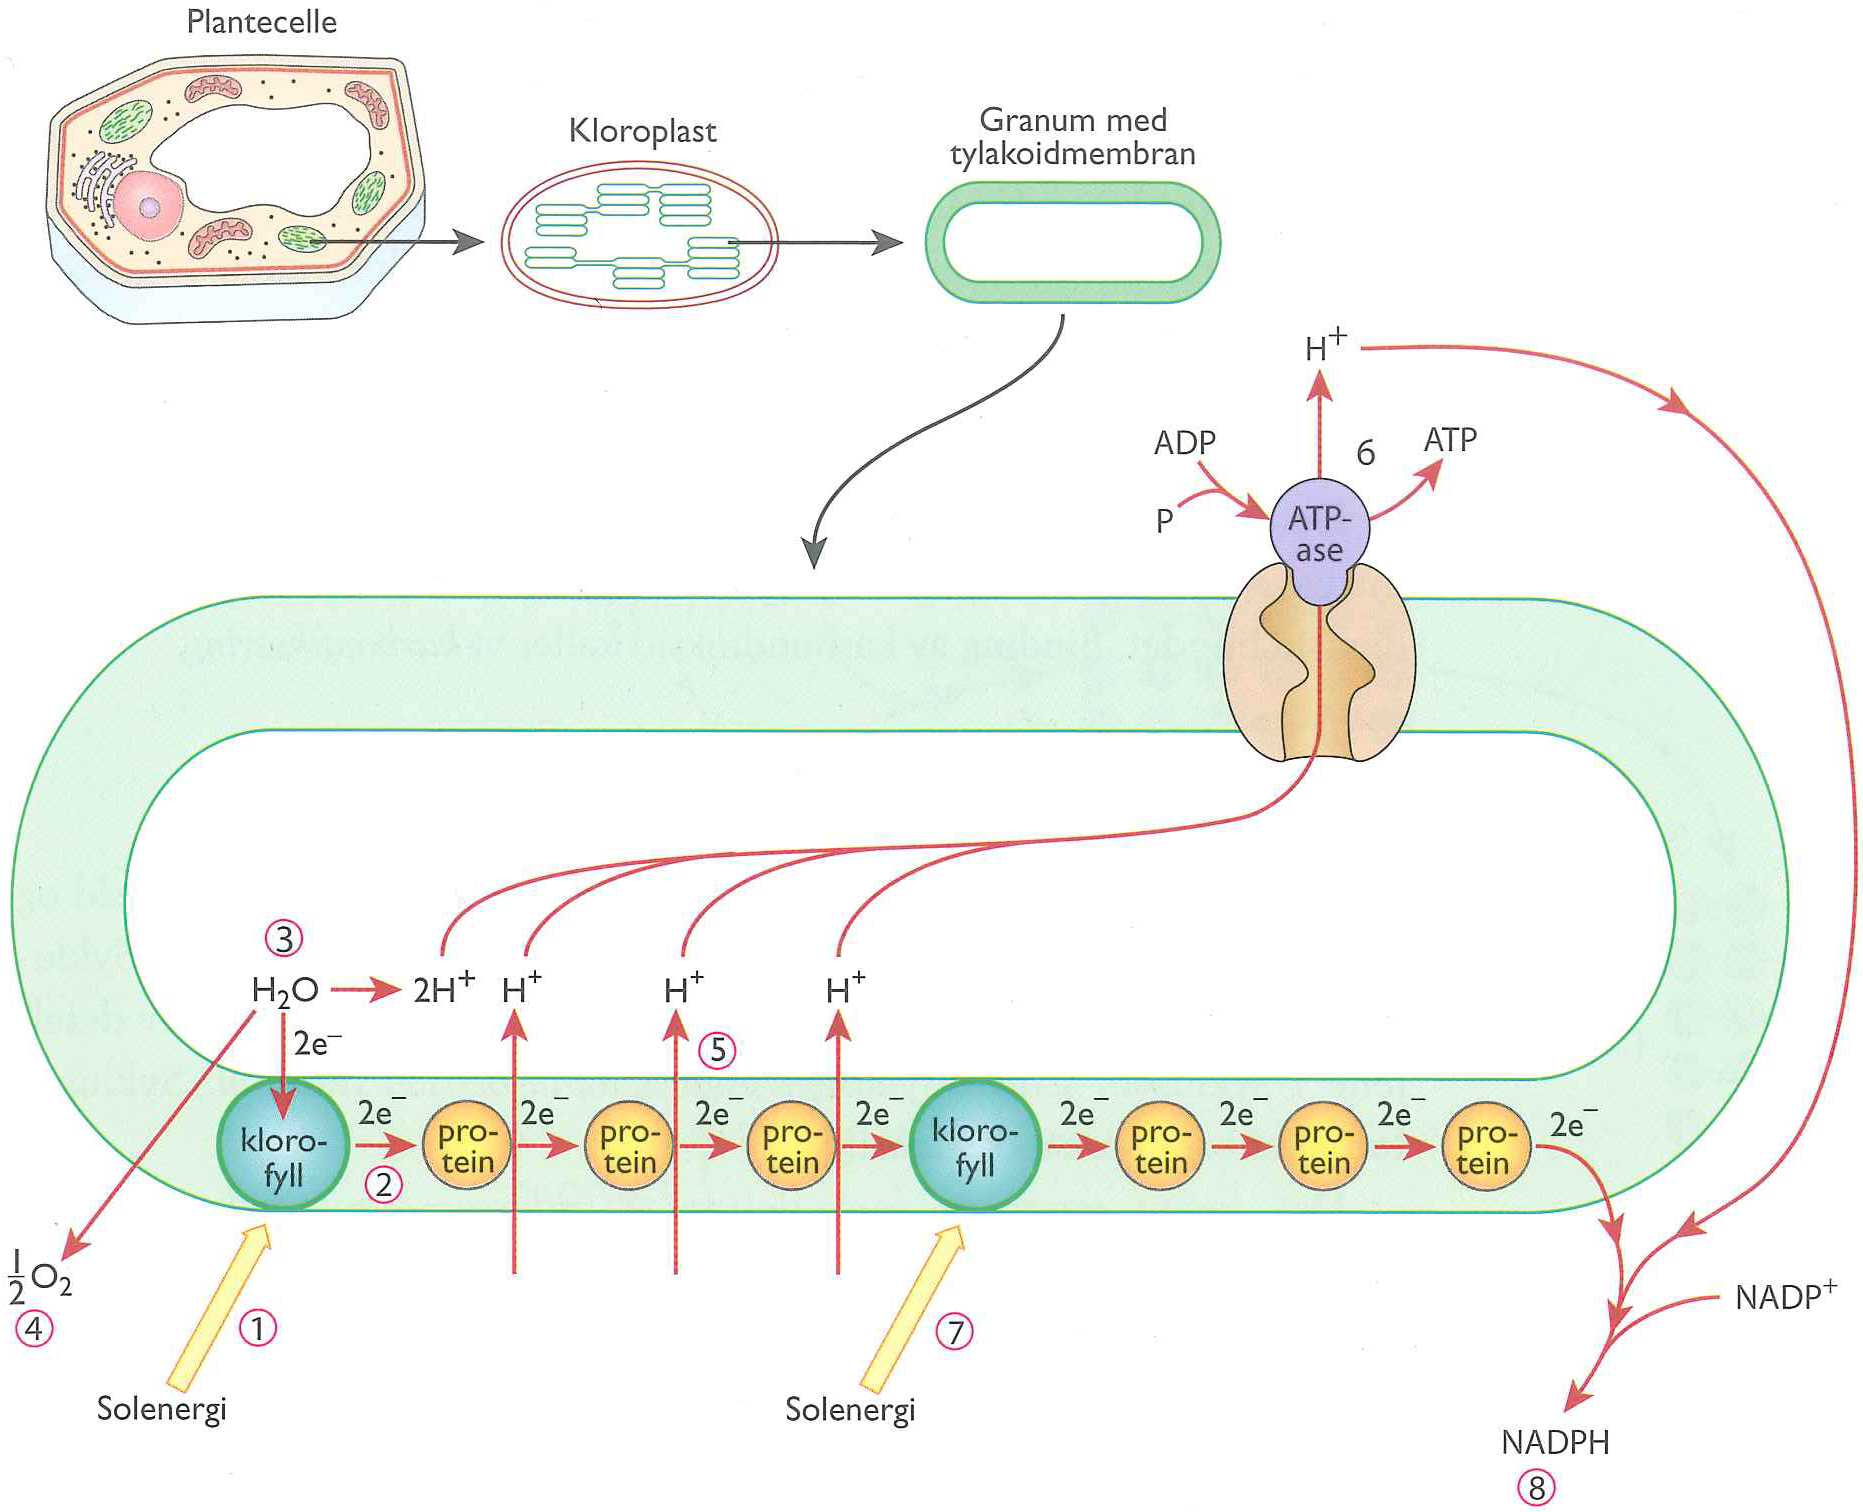
\includegraphics[width=\textwidth]{img/photosynthesis/light_dependent.png}
\caption{Illustration of PS1 and PS2 \citep{bios}}
\label{fig:photosystem}
\end{figure}

\subsection{Light-independent reaction (Calvin-cycle)}
This reaction works as a “sugar-factory”, collecting carbon dioxide and hydrocarbon in many cycles to make glucose. The process takes place in the stroma (see fig.~\ref{fig:chloroplast}), and requires the NADPH and ATP generated in the light-dependent reaction \citep{bi2}. 

The glucose produced can be used to generate other organic compounds such as other carbohydrates (e.g., starch and cellulose), proteins and lipids, depending on what the plant needs.

\subsection{External factors}
Many external factors affect the photosynthesis in plants. As photosynthesis is a relatively inefficient process, using only 8-10\% of the energy in sunlight, much research has gone into increasing photosynthesis to achieve greater conversion rates \citep{kirschbaum2011does}. The factors of significance are \citep{bios}:
\begin{itemize}
\item \ce{CO2} levels
\item Temperature
\item Light intensity and wavelength
\item Water
\end{itemize}
Each of these factors may be a limiting factor, or stressfactor, not enabling photosynthesis to reach its full potential. 

\subsubsection{\ce{CO2} levels}
\ce{CO2} is used in the light-independent reaction for making glucose. The atmosphere contains approximately 0.038\% \ce{CO2}, while the air in e.g., a classroom would most likely contain slightly higher values due to a high concentration of students exhaling \ce{CO2}. In a greenhouse \ce{CO2} levels can get too low, due to a high concentration of plants consuming \ce{CO2} and outputting \ce{O2}. The optimal concentration for most plants is between 0.015\% and 0.05\% \citep{bios}. 


\begin{figure}
        \centering
        \begin{subfigure}[b]{0.45\textwidth}
                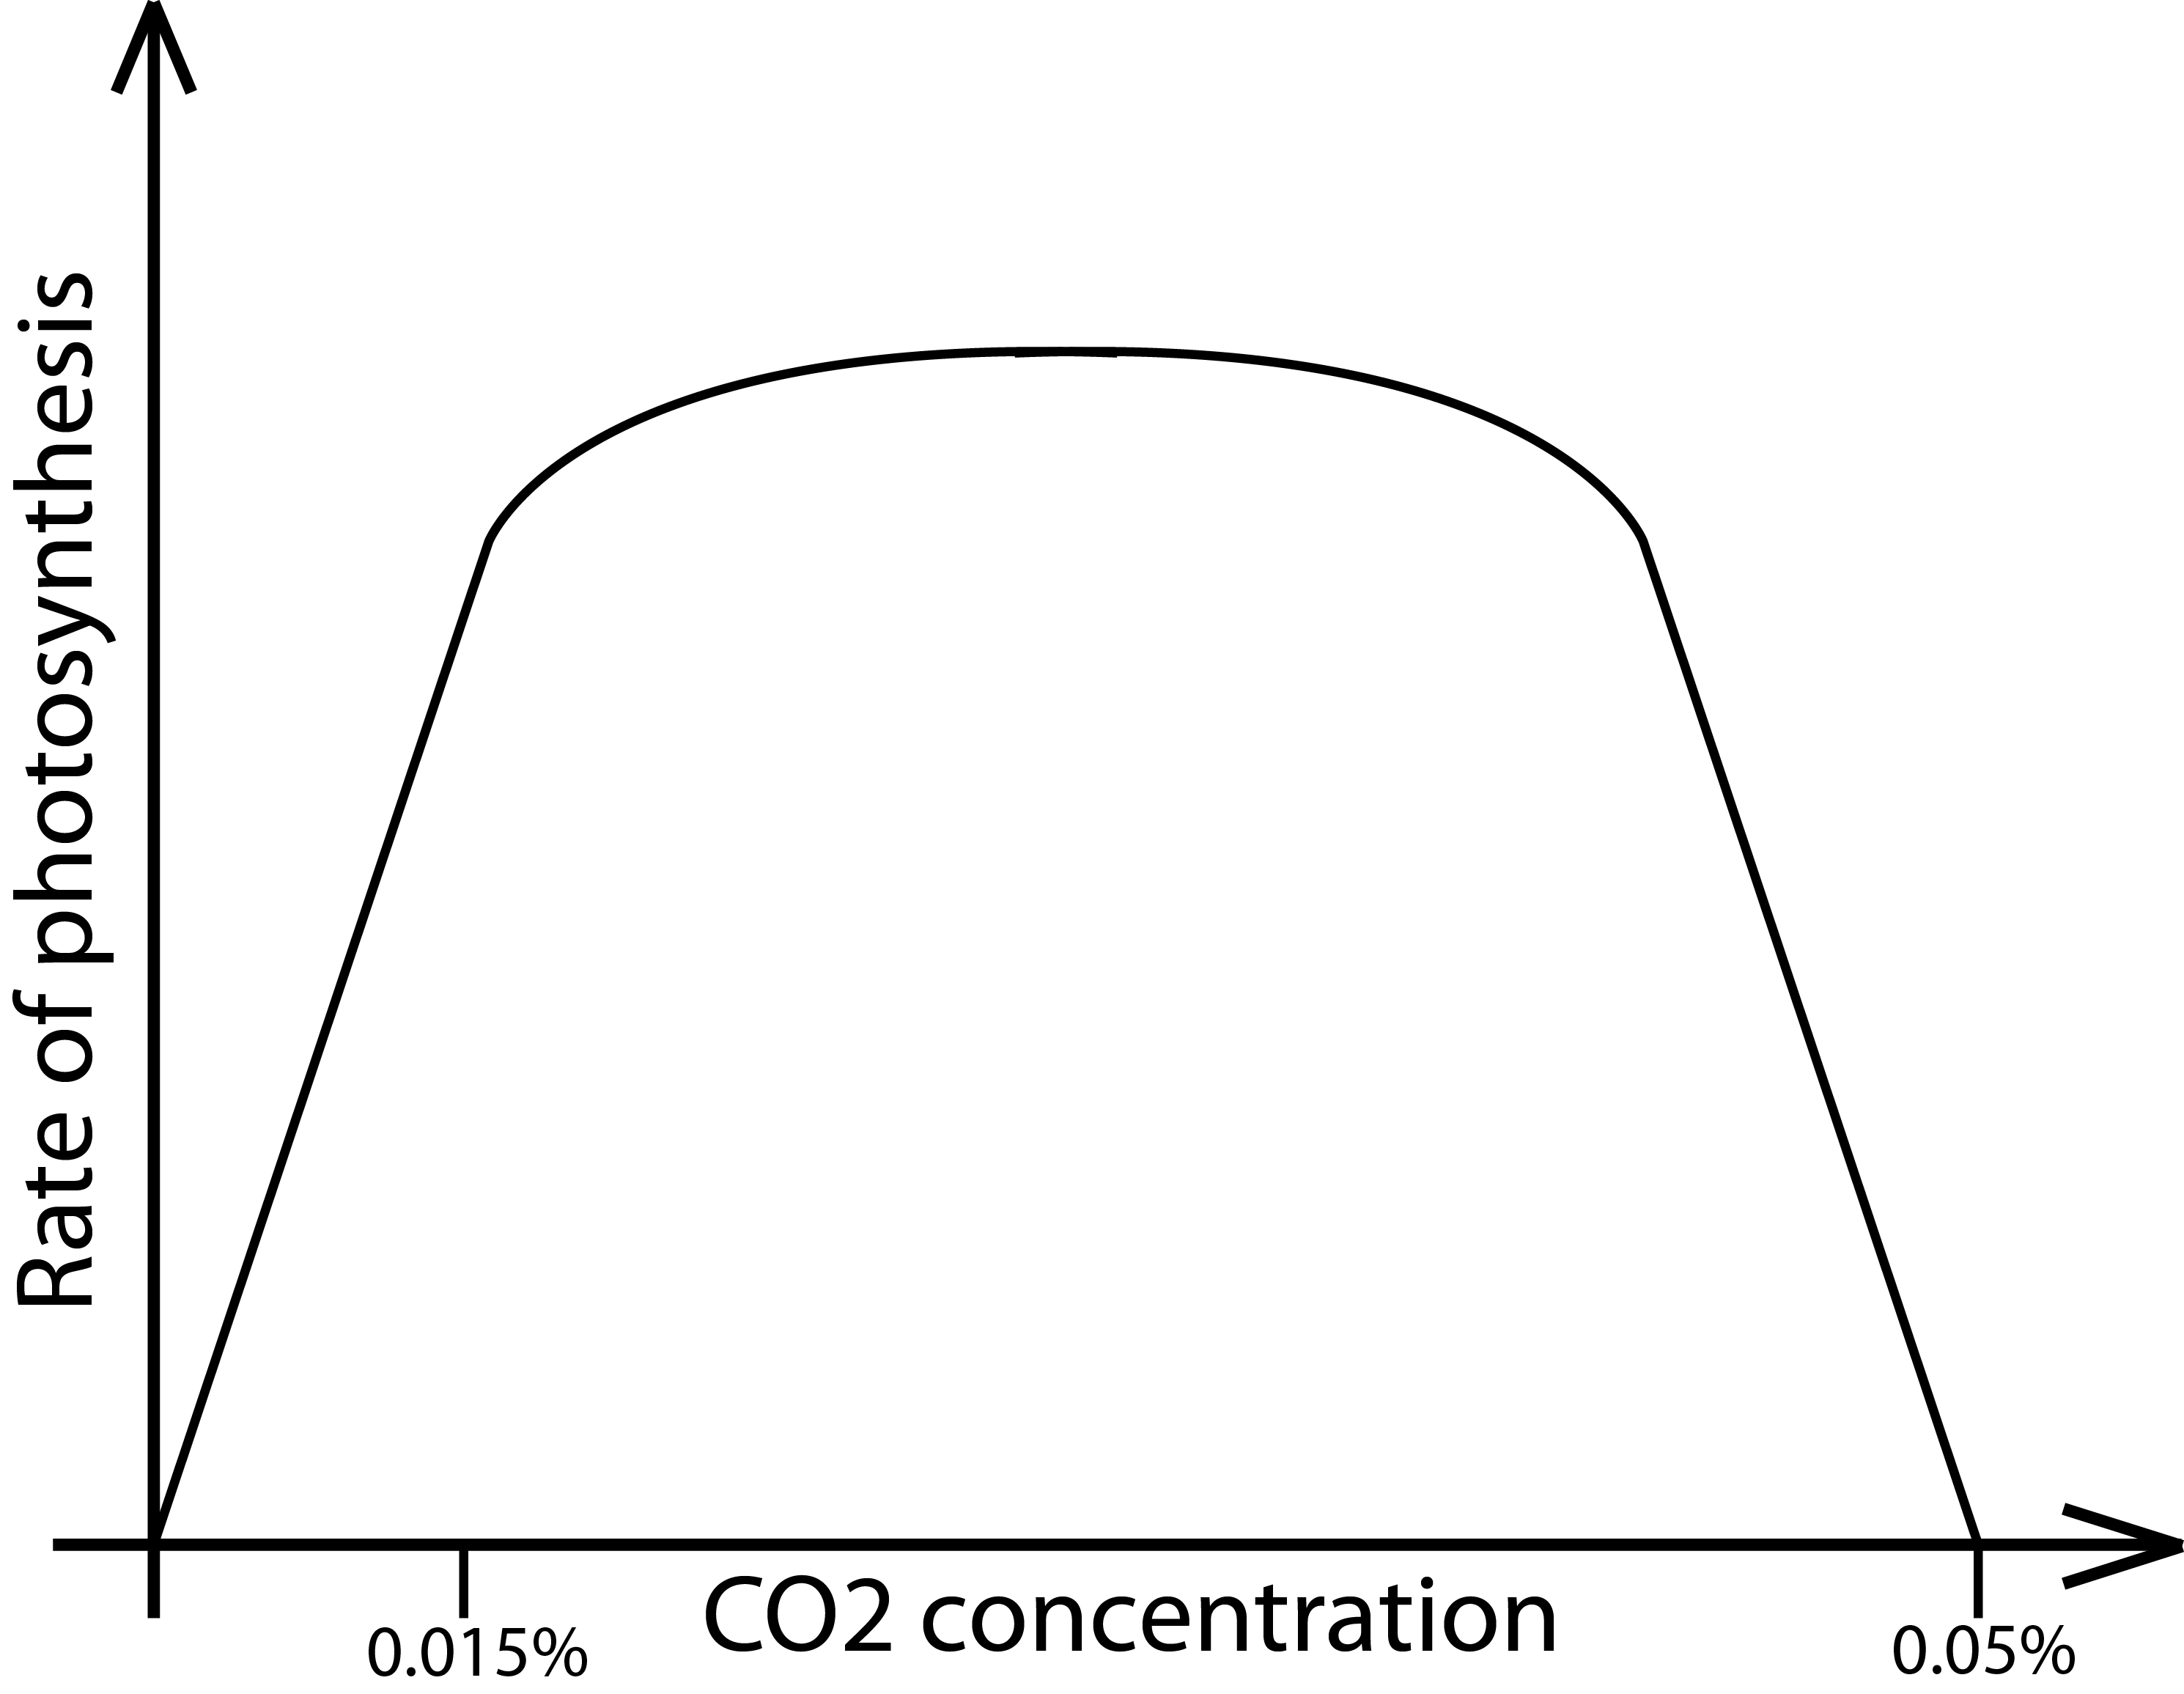
\includegraphics[width=\textwidth]{img/photosynthesis/co2.png}
                \caption{Effect of \ce{CO2} levels on photosynthesis}
                \label{fig:co2levels}
        \end{subfigure}
        ~~
        \begin{subfigure}[b]{0.45\textwidth}
                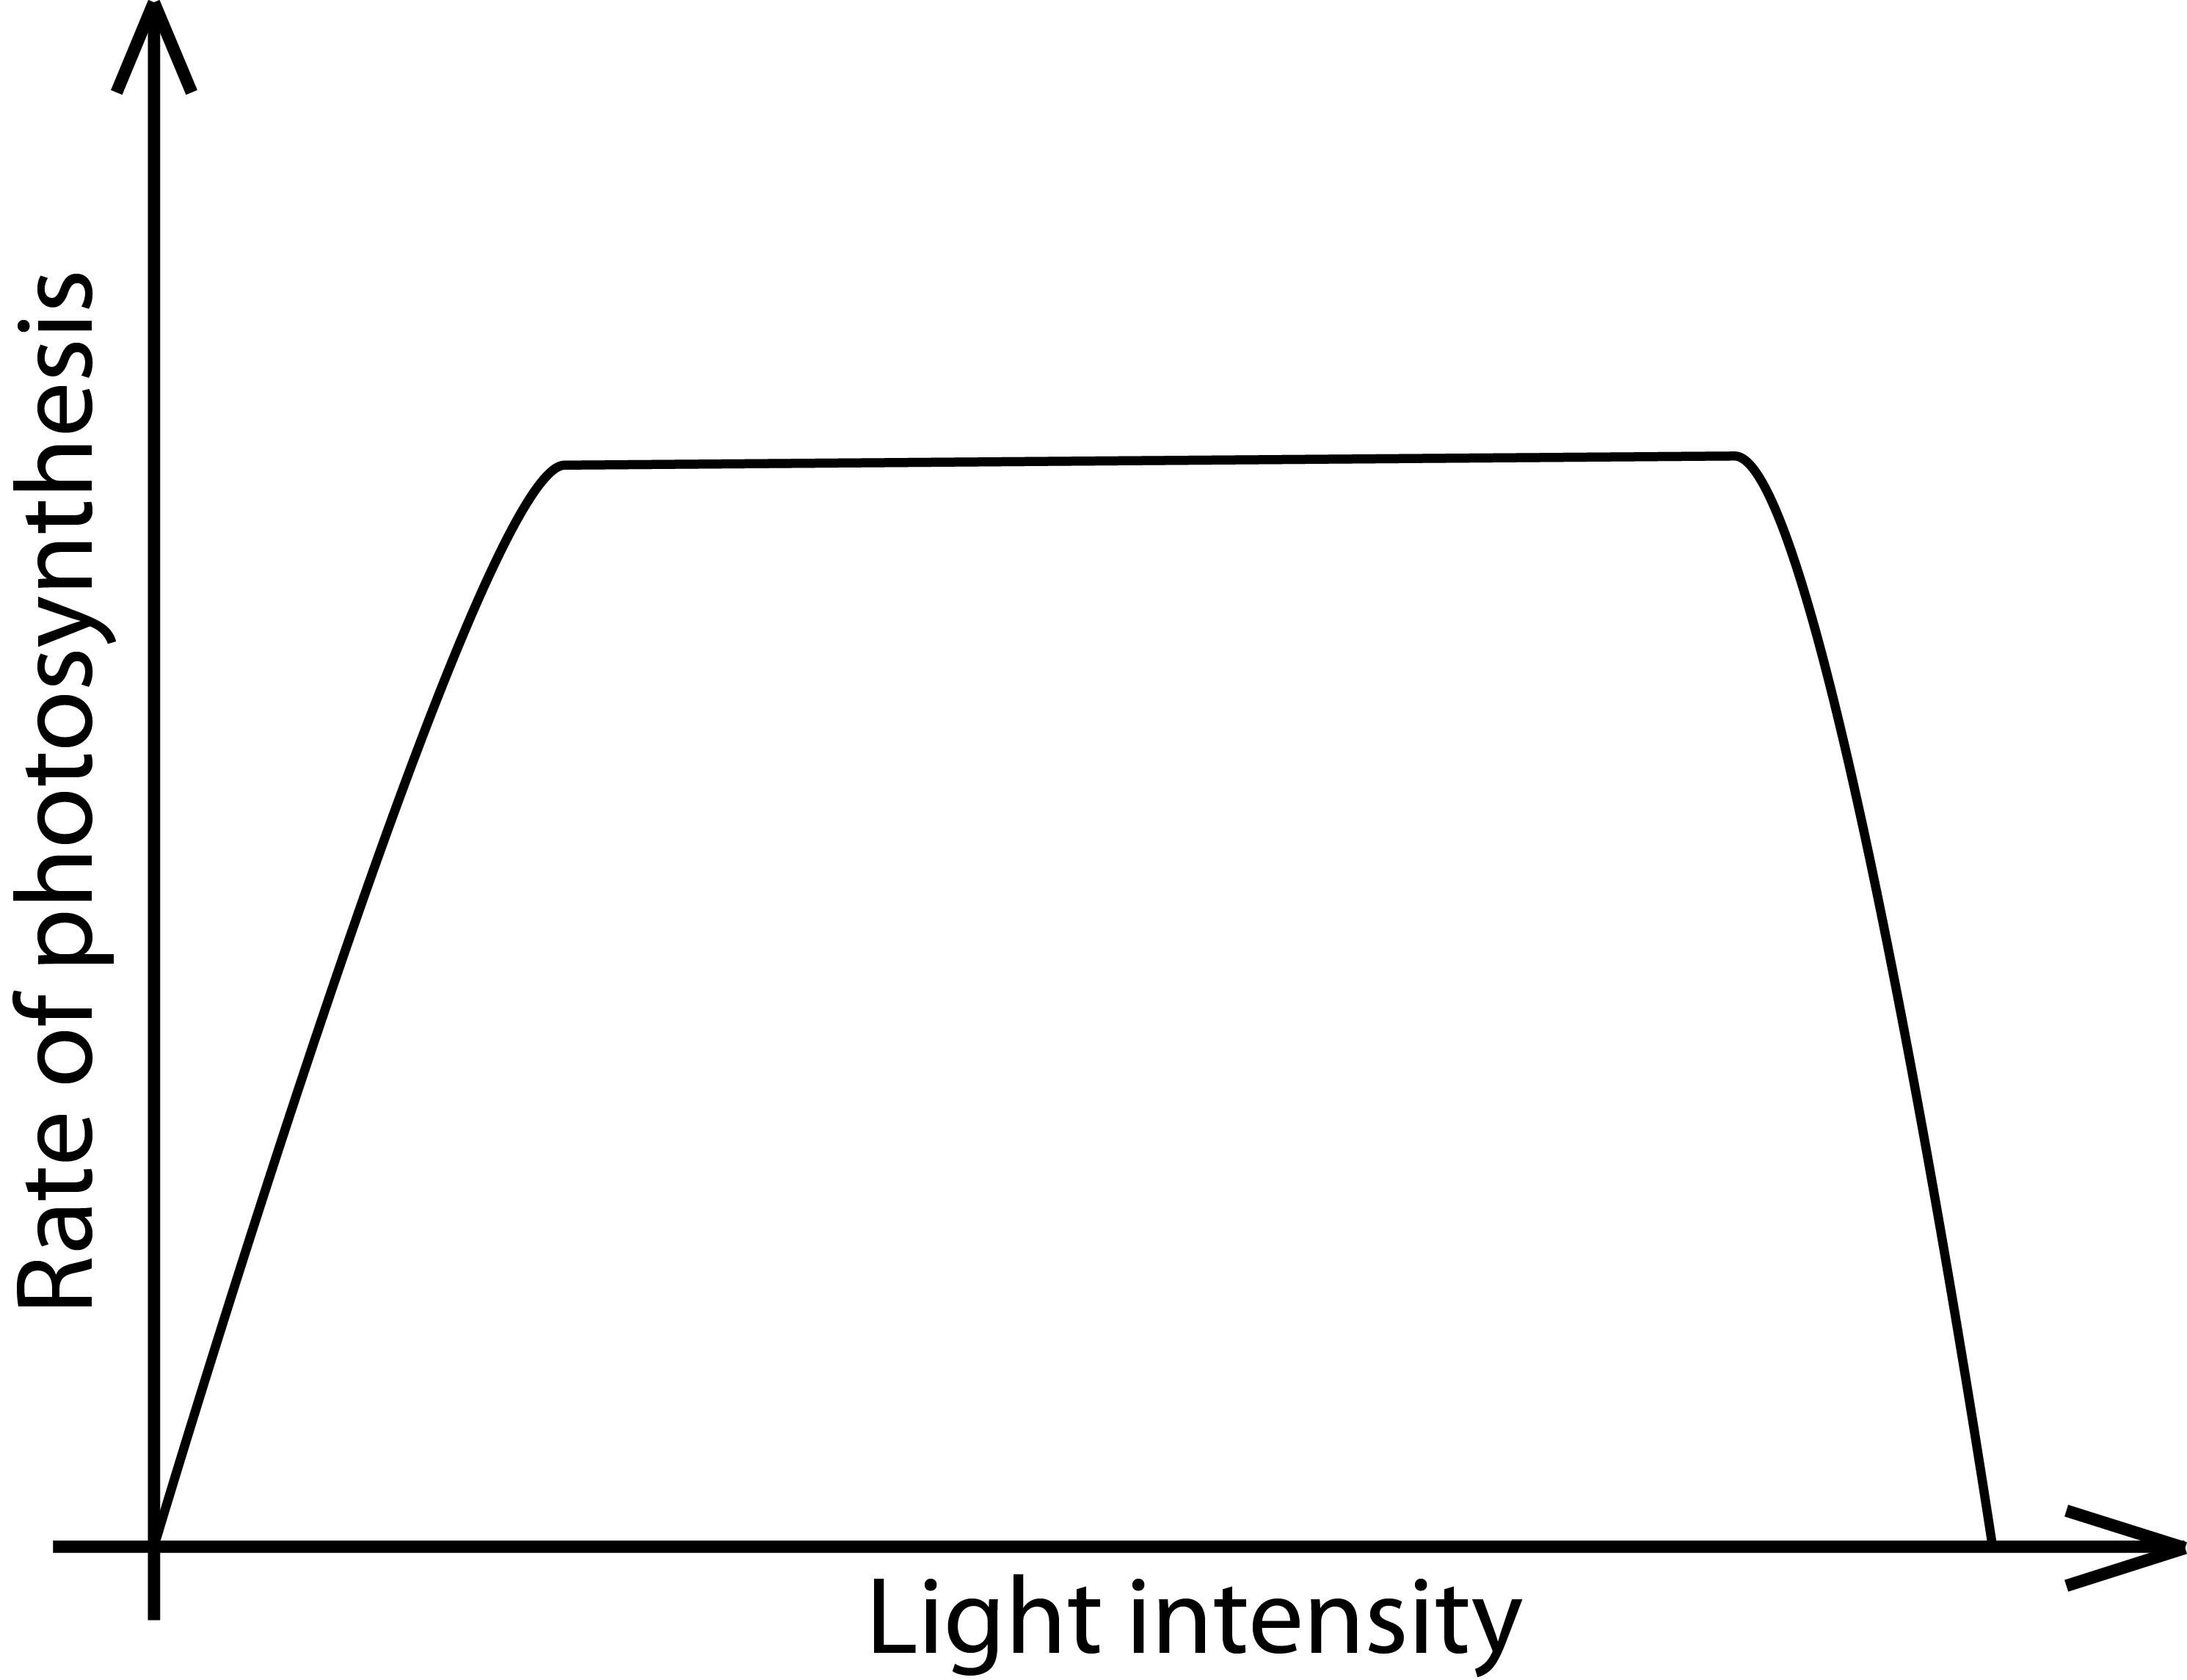
\includegraphics[width=\textwidth]{img/photosynthesis/light_intensity.png}
                \caption{Effect of light intensity on photosynthesis}
                \label{fig:lightintensity}
        \end{subfigure}
       
\end{figure}

\begin{figure}
\centering
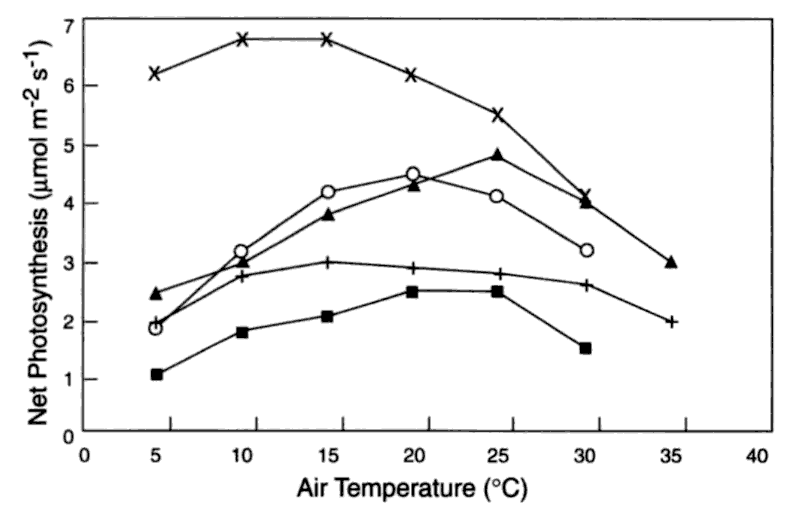
\includegraphics[width=0.75\textwidth]{img/photosynthesis/temperature_new.png}
\caption{Effect of temperature on photosynthesis. Species:
 \textit{\ensuremath{\blacktriangle} Pinus Taeda},  
\textit{\ensuremath{\bigcirc} Pinus Strobus}, 
\textit{\ensuremath{+} Pinus Sylvestris}, 
\textit{\ensuremath{\blacksquare} Picea Engelmanii}, 
\textit{\ensuremath{\times} Pinus Ponderosa}
\citep{hollinger1995external}
}
\label{fig:temperature}
\end{figure}

\subsubsection{Temperature}
All enzymes have an optimal temperature during which they function best \citep{bios}. This temperature may vary from species to species as plants grow in different climates, altitudes and seasons. If the temperature is too low or too high, the molecular structure of the enzymes may be destroyed.

\subsubsection{Light intensity and wavelength}
The different pigments in the light dependent reaction absorb light of wavelengths from mainly 400nm to 700nm. Chlorophyll b for instance absorbs blue light (450nm). If a plant with a high concentration of chlorophyll b is not given light of this wavelength, the electrons would not be excited and the reaction in photosystem 2 would not start.

Light intensity also plays a role in this reaction. In low light conditions, there is not enough energy available to excite the chlorophyll molecules, in order to move electrons as needed in PS2. In optimal light conditions, the production is light-saturated meaning that all the chlorophyll molecules are exciting electrons. In too strong light conditions, the chloroplasts may burn out from the heat and die.  

\begin{figure}
        \centering
        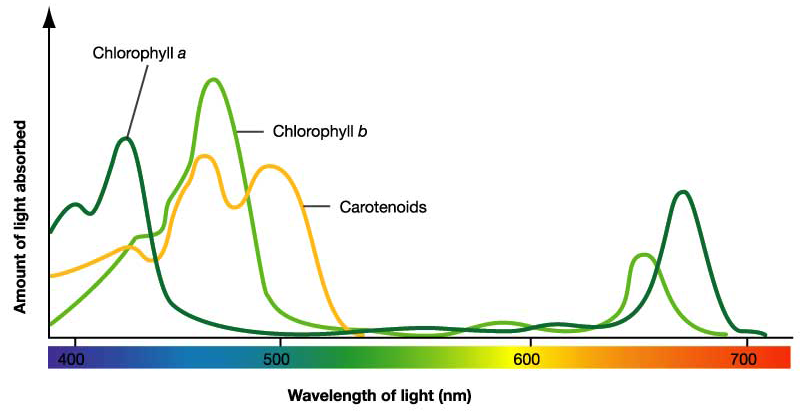
\includegraphics[width=0.8\textwidth]{img/photosynthesis/absorption-spectrum.png}
        \caption{Wavelengths of light absorbed by different pigments}
        \citep{uicbiology}
        \label{fig:wavelengthabsorbtion}
\end{figure}

\subsubsection{Water}
Water is used in both the light-dependent and light-independent reactions, but is seldom a limiting factor. If water-levels are low and the evaporation-rate is high, most plants will close the leaves to minimize water-loss. This makes the plant unable to absorb \ce{CO2} and photons, which leads to plant reduction \citep{bi2}. Water shortage is only a problem in itself when the plant's cells dries out, leading to the stem and tissue collapsing. 


% \section{Koubachi} %Dette er noe dritt! fuck Koubachi. jævla sveitsere
% \begin{figure}
%         \centering
%         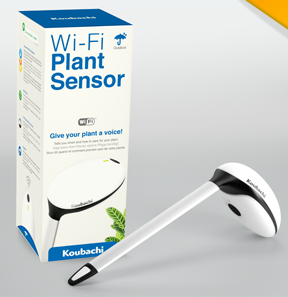
\includegraphics[width=0.4\textwidth]{img/koubachi/sensor.png}
%         \caption{Koubachi}
%         \label{fig:koubachi}
% \end{figure}

% Koubachi is a commercial plant monitoring system developed by a company by the same name. The functioning steps of Koubachi is divided in 3: 1.)\emph{Measure}, 2.) \emph{Analyze} and 3.) \emph{Display}. This is done through a sensor unit, the \emph{Koubachi Plant Care Engine (PCE)} and user interfaces in form of a web application and an iOs application \citep{koubachi}. As seen in figure~\ref{fig:koubachidata}, the sensor unit measures soil moisture, temperature and light. The web interface displays the last of the transmitted readings. The koubachi transmits data once every 24 hours in order to save battery life. It does however read data every tenth minute, so the PCE has access to how the environment change over the span of each day.

% The PCE is basically an API with the functionality of storing data from sensors, analyzing the data and distributing data and instructions on how and when to care for the plant. Based on plant care models developed by biologists through greenhouse experiments, the PCE can determine the needs of any plant species. Thus, combining the data gathered by the sensor unit with the plant care model, Koubachi provides notifications about how and when to care for your plant. An example of this can be seen in figure~\ref{fig:koubachigraph}, where a graph of light measurements the preceding week i displayed together with a note that \emph{Gretches has too much shade} (Gretches beeing the name of the plant). Apart from obvious technical differences, this seems to be the main divergence from Monoplant; Koubachi is not only presenting data, it is also providing an opinion if the plant is comfortable or not, even suggesting measures for care taking.

% \begin{figure}
%         \centering
%         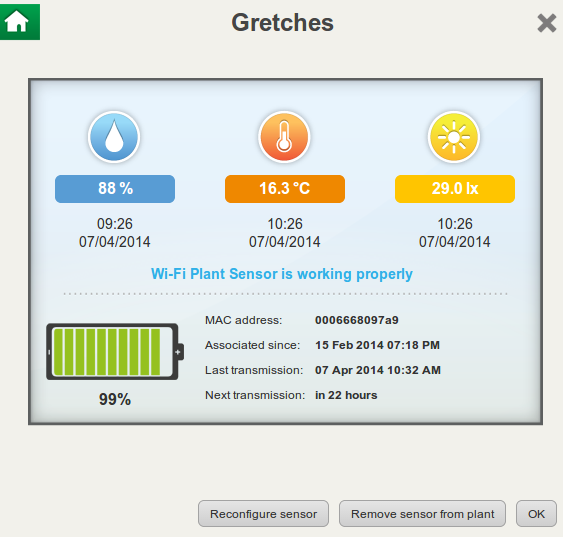
\includegraphics[width=0.8\textwidth]{img/koubachi/instantdata.png}
%         \caption{Last data from web interface}
%         \label{fig:koubachidata}
% \end{figure}

% \begin{figure}
%         \centering
%         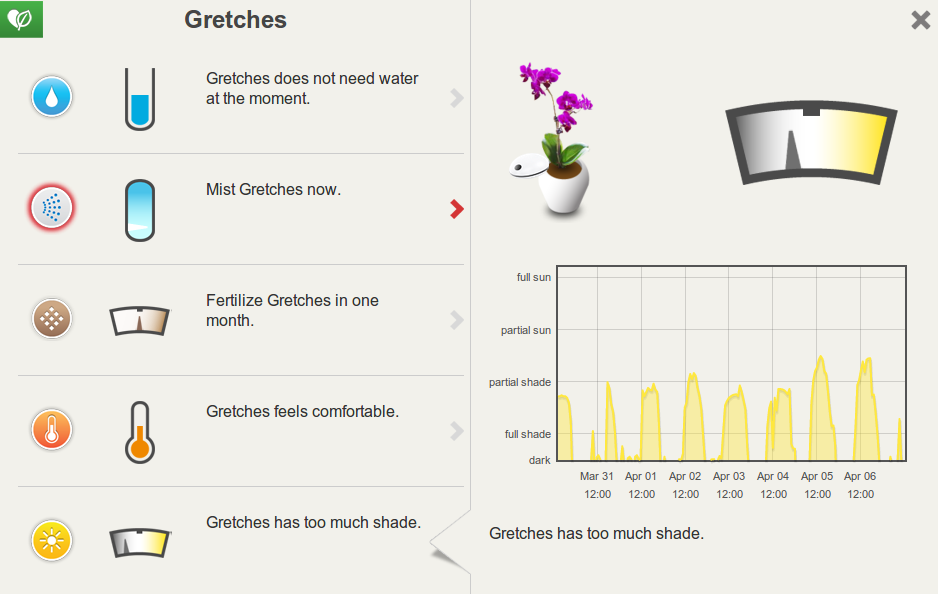
\includegraphics[width=0.8\textwidth]{img/koubachi/lightgraph.png}
%         \caption{Light graph from web interface}
%         \label{fig:koubachigraph}
% \end{figure}


%!TEX root = ../document.tex
\chapter{Technical architecture and programming}
In this chapter we will present the technical aspects of our learning tool, Monoplant. We will explain the rationale for the design choices made, and go into detail on some of the more advanced parts of the system. We will not give an in-depth explanation of all the technicalities, but rather present an overview to give the reader some background to understand the learning opportunities built into the system. First we will give a short introduction of some related applications, then we present Monoplant based on its architectural structure. First addressing the data collection, then data processing and storage, and finally the user interface.

\section{Related applications}
When starting our work with Monoplant, a review of existing technology was done. While there is some commercial plant monitoring systems, the major part of existing projects where characterized by the "do it yourself"-style (DIY). The latter involved use of prototype platforms such as Arduino, where the makers provided instructions for how people could make their own version of their system. Projects reviewed included twittering plants, plants making phone-calls, self-watering plants and gardening Arduinos \citep{botanicalls,selfwater,garduino}. All the DIY projects where focused on responding to variable changes around the plant, and can therefore be categorized as automated systems. 

The commercial products reviewed where Koubachi and Twine \citep{koubachi,twine}. Twine being a monitoring system for usage in the home and Koubachi a plant monitoring system with a focus on helping people take care of their plants. The systems reviewed proved that there is an interest for plants and for using technology to bridge the gap in human-plant interaction. However, the tools are not concerned with learning, and are mostly making use of 1-3 environmental variables, paying no attention to capturing visual images of plants. Monoplant is therefore a more complex system, and the systems reviewed did not inform our design to any large degree.

% \section{Koubachi} %Dette er noe dritt! fuck Koubachi. jævla sveitsere
% \begin{figure}
%         \centering
%         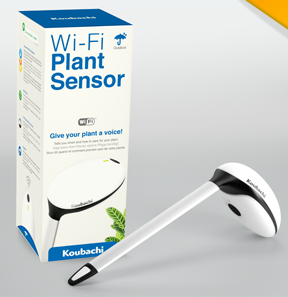
\includegraphics[width=0.4\textwidth]{img/koubachi/sensor.png}
%         \caption{Koubachi}
%         \label{fig:koubachi}
% \end{figure}

% Koubachi is a commercial plant monitoring system developed by a company by the same name. The functioning steps of Koubachi is divided in 3: 1.)\emph{Measure}, 2.) \emph{Analyze} and 3.) \emph{Display}. This is done through a sensor unit, the \emph{Koubachi Plant Care Engine (PCE)} and user interfaces in form of a web application and an iOs application \citep{koubachi}. As seen in figure~\ref{fig:koubachidata}, the sensor unit measures soil moisture, temperature and light. The web interface displays the last of the transmitted readings. The koubachi transmits data once every 24 hours in order to save battery life. It does however read data every tenth minute, so the PCE has access to how the environment change over the span of each day.

% The PCE is basically an API with the functionality of storing data from sensors, analyzing the data and distributing data and instructions on how and when to care for the plant. Based on plant care models developed by biologists through greenhouse experiments, the PCE can determine the needs of any plant species. Thus, combining the data gathered by the sensor unit with the plant care model, Koubachi provides notifications about how and when to care for your plant. An example of this can be seen in figure~\ref{fig:koubachigraph}, where a graph of light measurements the preceding week i displayed together with a note that \emph{Gretches has too much shade} (Gretches beeing the name of the plant). Apart from obvious technical differences, this seems to be the main divergence from Monoplant; Koubachi is not only presenting data, it is also providing an opinion if the plant is comfortable or not, even suggesting measures for care taking.

% \begin{figure}
%         \centering
%         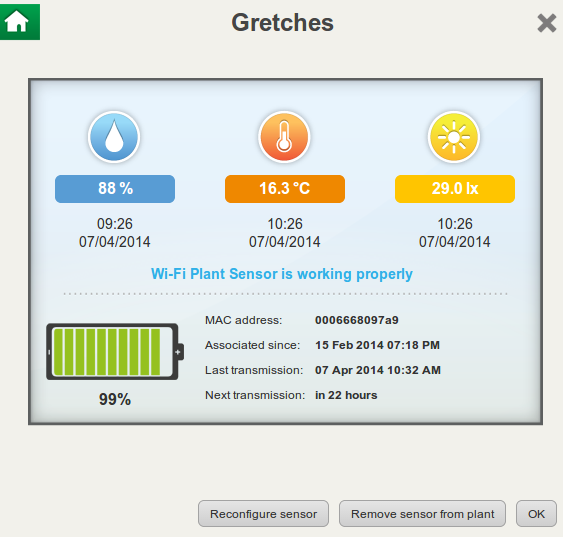
\includegraphics[width=0.8\textwidth]{img/koubachi/instantdata.png}
%         \caption{Last data from web interface}
%         \label{fig:koubachidata}
% \end{figure}

% \begin{figure}
%         \centering
%         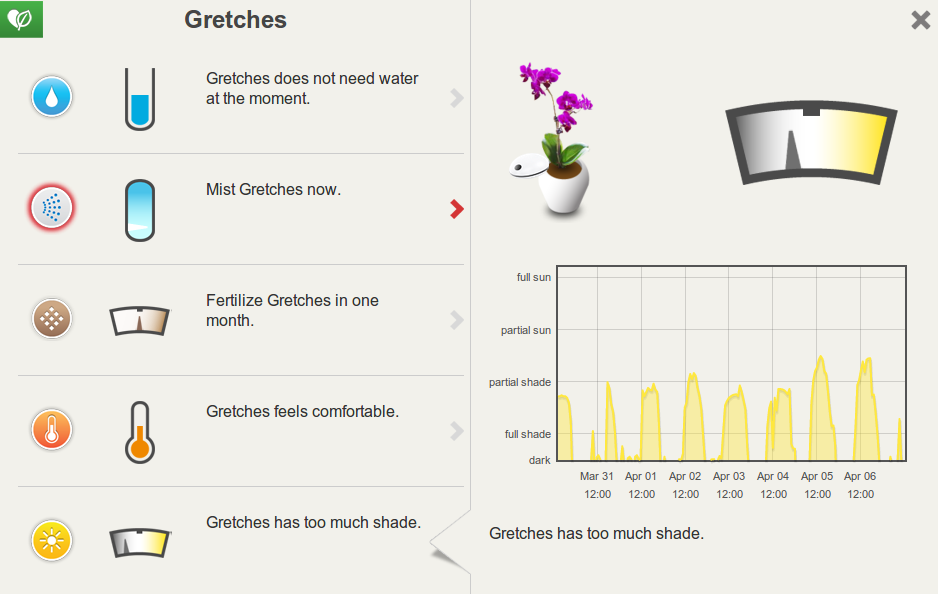
\includegraphics[width=0.8\textwidth]{img/koubachi/lightgraph.png}
%         \caption{Light graph from web interface}
%         \label{fig:koubachigraph}
% \end{figure}


\begin{figure}
\centering
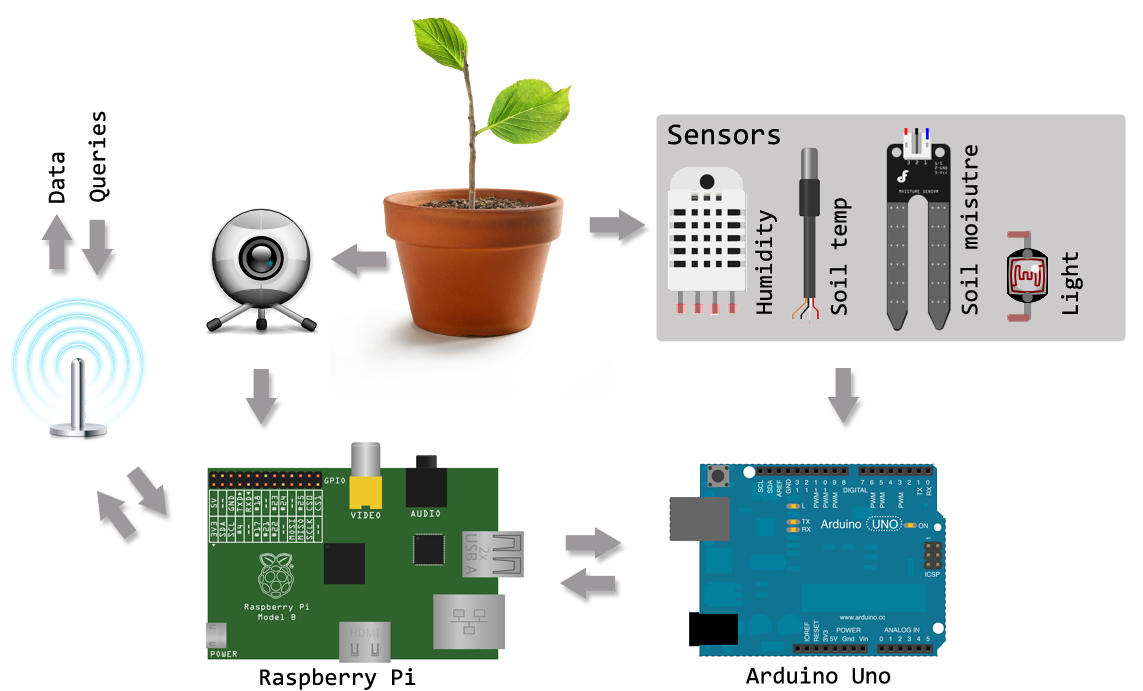
\includegraphics[width=1\textwidth]{img/hardware/application.png}
\caption{High-level illustration of the physical hardware components in Monoplant}
\label{fig:application}
\end{figure}

\section{Plant data collection}
At the lowest level in the information hierarchy is the hardware and software responsible for capturing and uploading environmental data regarding the plant. Like a patient in a hospital, the plant is connected to a range of sensors, each responsible for reading a specific variable that is important for the plant's functioning. These variables are sent to a computer, processed, and uploaded to the next level in the data hierarchy. In the following sections we will follow the data on its way from the plant's physical location to the "cloud" and the user.

\subsection{Sensors}

\def\arraystretch{1.8}
\begin{table}
	\begin{tabular}{@{}lp{250pt}@{}}\toprule
	Sensor               & Description \\ \midrule                                                                                                  
	TSL2561              & Digital luminosity sensor. Measures light in lux from 300-1100nm.                                            \\ 
	RHT03                & Digital humidity and temperature sensor. Measures relative humidity and temperature in Celsius.              \\ 
	DS18B20              & Digital waterproof temperature sensor. Measures temperature in Celsius.                                       \\ 
	DFRobot sku:sen0114  & Analog soil moisture sensor. Returns values between 0 and 900 depending on electrical conductivity of soil.  \\ \bottomrule
	\end{tabular}
	\caption{Sensors used in the application}
\end{table}


With the advent of the "internet of things", sensors are becoming available in many different forms and packages. They are cheap and can be used as modular building blocks in a wide range of applications, from automating tasks such as keeping a steady indoor-temperature, to measuring variables that humans cannot see. 

The sensors are able to capture information concerning the environment and transform it to data variables, which we can store and categorize. In total there are five different sensors connected to the plant, or in the plant’s vicinity: soil moisture, soil temperature, air temperature, humidity, and light intensity. 


%(write something about the sensortag)

The sensors we have used in this project are analogous to a volume controller on an amplifier. On an amplifier one can adjust the volume by varying the resistance in the signal going to the speakers. If we turn the volume up, the resistance goes down, and if we turn the volume down, the resistance goes up. Sensors work in the same way, but instead of controlling resistance with a volume knob, it is controlled by light, moisture or other environmental variables. 

To exemplify let's look at temperature sensors, or "thermistors". They vary their resistance in relation to the temperature. Since we already know how many volts we are sending to the thermistor on the one end, we can use the amount of volts we get back to calculate the resistance. In our application this is done by a voltage divider, which uses a formula as follows: 

\begin{equation}
V_{out}=\frac{R_{2}}{R_{1}+R_{2}}\cdot V_{in} 
\label{eq:vdiv1}
\end{equation}
Where $V_{out}$ is voltage out, $V_{in}$ is voltage in, $R_{1}$ is a given resistance, and $R_{2}$ is the resistance we want to calculate. For this example let's assume that $V_{in} = 5_{v}$, $V_{out} = 2_{v}$, and $R_{1} = 1K\Omega$. We solve this equation with regard to $R_{2}$
\begin{equation}
R_{2} = \frac{V_{out} \cdot R_{1}}{V_{in}-V_{out}}
\end{equation} 

\begin{equation}
R_{2} = \frac{2_{v} \cdot 1000\Omega}{5_{v}-2_{v}}
\end{equation} 

\begin{equation}
R_{2} = \frac{2000\Omega}{3}
\end{equation} 

\begin{equation}
R_{2} = 667\Omega
\end{equation} 

Then we can see that the calculated resistance is 667$\Omega$. This value can then be mapped to the correct unit of measure, in this case Celsius or Fahrenheit. 

As we are using digital sensors, all of these calculations are done internally in the sensors, and coded into a digital signal. This signal is then passed onto the next unit in our system, the Arduino.  

\subsection{Arduino}
%(Write about embedded systems. What other alternatives are there to the Arduino? )

Arduino is an open-source prototyping platform that makes it easy to interface low-level electronics (i.e., sensors) with higher-level electronics (i.e., computers). The core part of the Arduino is an Atmel\texttrademark Atmega microcontroller, which can be programmed by a computer over a USB port, using the Arduino programming language and the Arduino development environment \citep{Arduino}.

%We have used an Arduino Uno that has 13 digital input output pins (GPIO), five analog inputs, i2c inputs, and a USB port for serial communication. The soil temperature sensor and the temperature and humidity sensor are connected to the digital inputs through a 1K(ohm) pullup resistor. The pullup resistor is used to keep the voltage sent to the Arduino from fluctuating when the sensor is not sending any data. The TSL2561 luminosity sensor is connected to the A4/SDA and A5/SDL ports of the Arduino as it communicates over the i2c protocol. And the DFRobot soil moisture sensor is connected to A3 (Analog input 3) as it outputs analog voltage.  

\begin{figure}
\centering
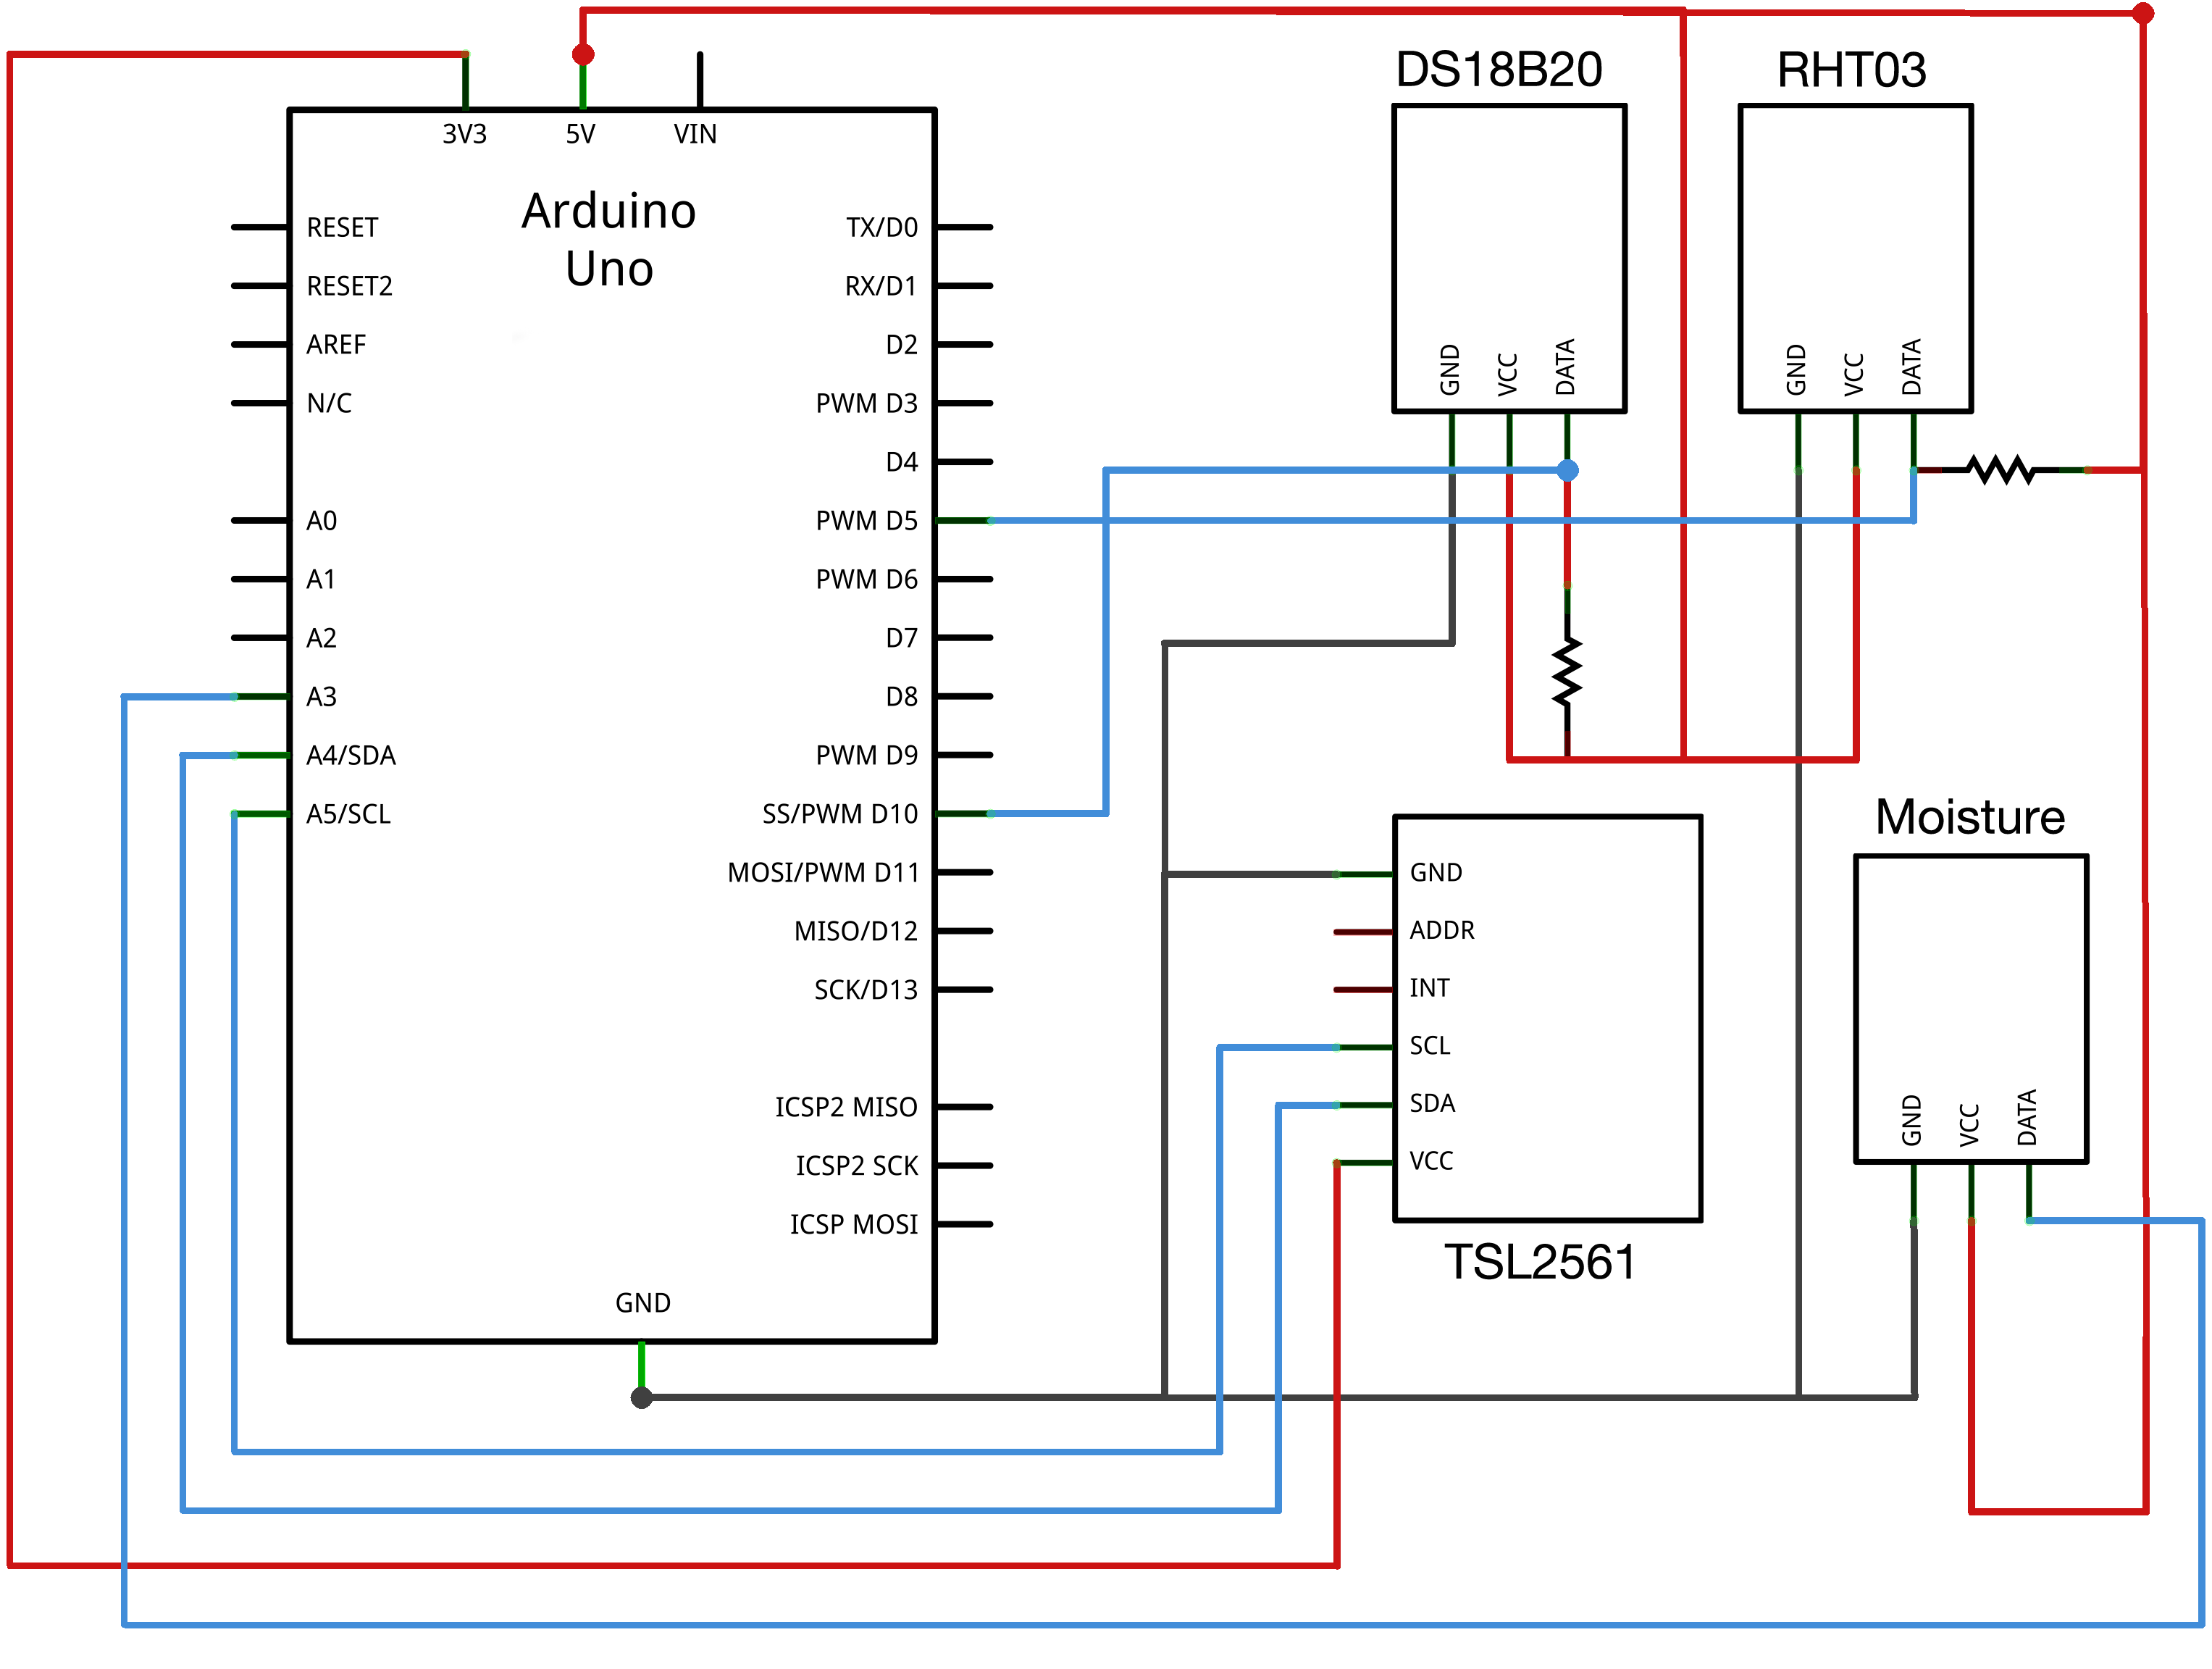
\includegraphics[width=1\textwidth]{img/hardware/Arduino_and_sensors_schem.png}
\caption{Schema diagram of Arduino sensor wiring. Pull-up resistors on the data line of the temperature sensors.} %The TSL2561 light sensor communicates over the i2c protocol (SDA,SCL), and the soil moisture sensor connects to analog input}
\label{fig:Arduino}
\end{figure}

The community surrounding Arduino is quite large, and we have therefore been able to find pre-written libraries for communicating with the different sensors. This has simplified the task of converting the digital signal to the correct units (Celsius, relative humidity, lux). 

In the case of the soil moisture sensor, it measures conductivity in the soil, and does not output moisture levels in any kind of universal measuring unit. But the conductivity measured in the soil is repeatable and proportional to the moisture level. Therefore we measured the resistance in air (high resistance), and in water (low resistance), and let these be the high and low points of a new unit called arbitrary moisture units (AMU) \citep{ch00ftech}.

The code residing in the Arduino runs a simple loop where it waits for a special character sent over serial communication through USB. If it receives this character it reads all the sensor values, and sends them back to the next device in the Monoplant system: the Raspberry Pi

\subsection{Raspberry Pi}
%(Why Raspberry? Beagleboard?)
The Raspberry Pi is a “cheap, accessible, programmable computer” \citep{Raspberrypi}, which is roughly the size of a credit card. Our model was released in early 2012 and contains two usb ports, audio and a SD-card slot. We have connected a wireless network adapter, a high-definition webcam, a powered USB-hub, and an Arduino to the Raspberry. The operating system running on it is a port of Debian Linux optimized for the Raspberry, called Raspbian. 

\begin{figure}
\centering
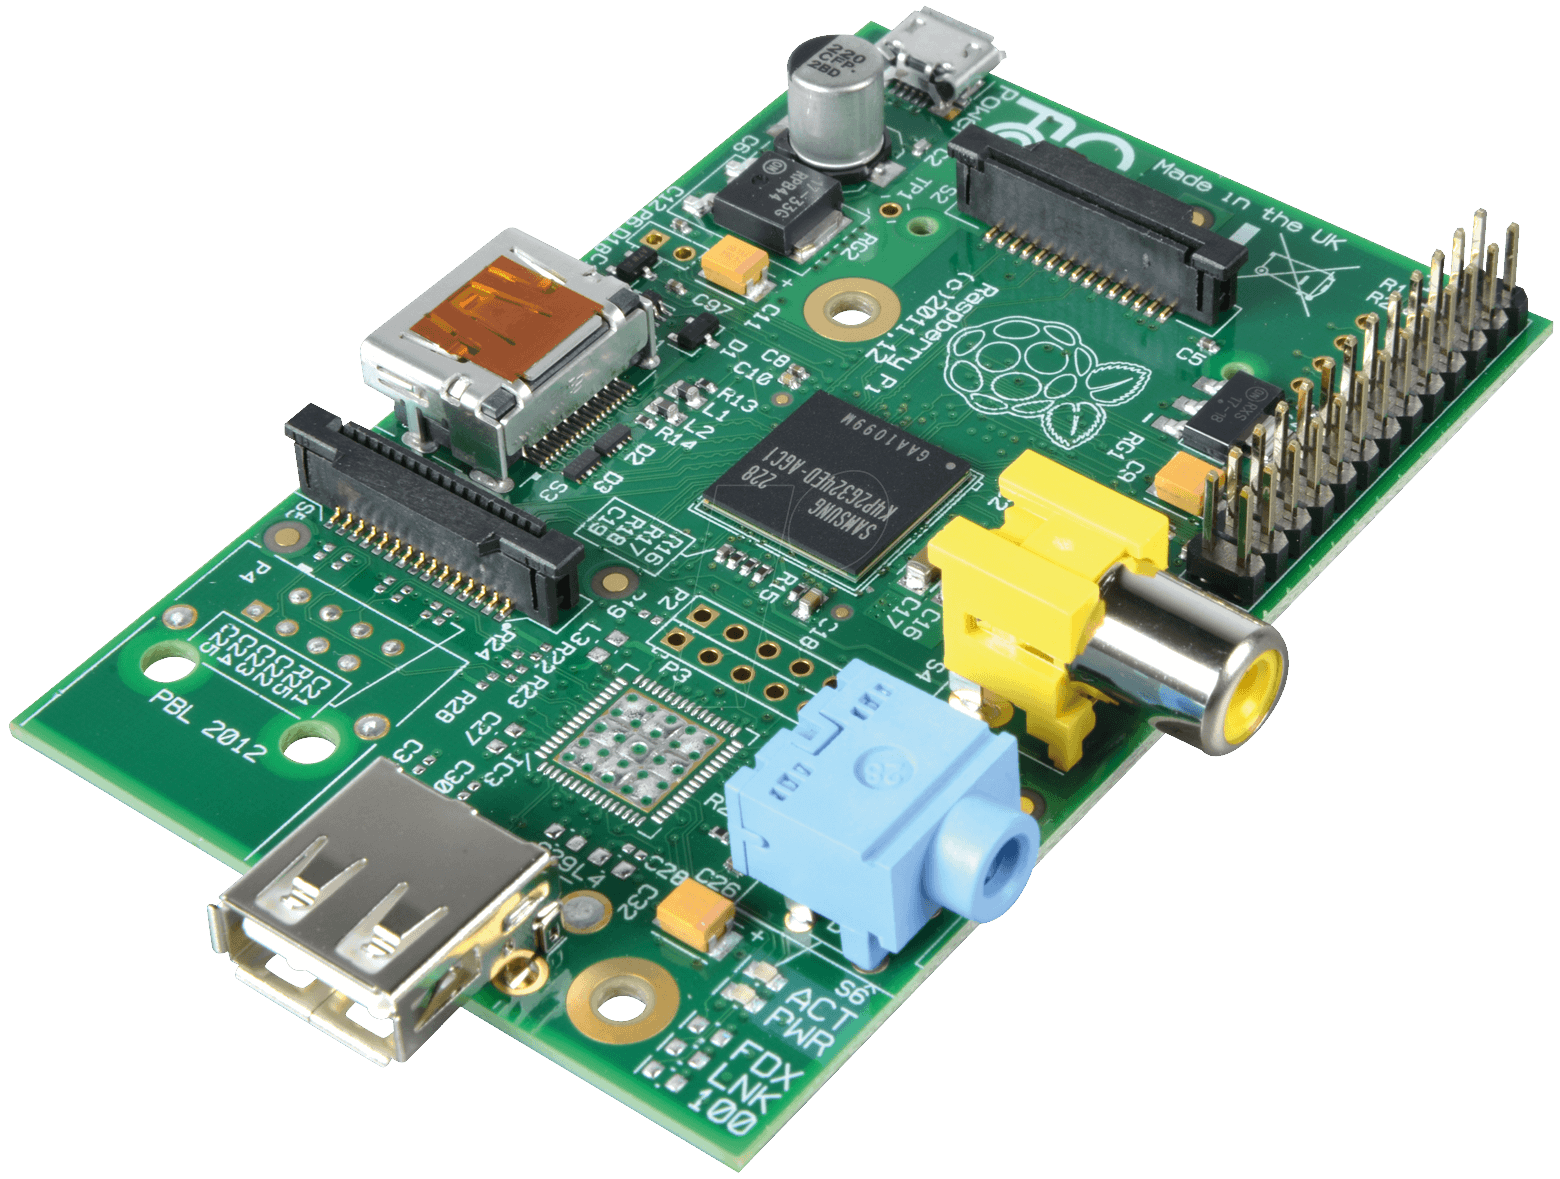
\includegraphics[width=1\textwidth]{img/hardware/raspberry.png}
\caption{Raspberry Pi}
\label{fig:Raspberry}
\end{figure}

%The GPIO-pins on the Raspberry works almost in the same fashion as the Arduino's digital input output pins. Thus we could in theory simplified the hardware by omitting the Arduino. The main reason for not doing this is that the Raspberry does not have an analog to digital converter (ADC). Therefore we would have to make a complex circuit involving an ADC to interface the Raspberry with the soil moisture sensor. In addition, we would most likely face timing issues. When we ask the digital sensors for data, they send the response immediately. If the unit receiving is not available to read the data, it gets lost. This can be a problem when using a high-level computer, as it performs multiple tasks in addition to reading sensordata. 

\subsubsection{Operation}
After booting up, a bash-script running an endless loop is called. The script snaps a photo of the plant using the webcam, and then runs a python-script responsible for collecting sensordata (see fig.~\ref{fig:Raspberrycode}). Since we sometimes can get erroneous values from the sensors, we read 15 values and upload the median value. These values, along with the photo captured by the webcam, are then passed on to the next logical unit in the Monoplant system. 

%http://en.wikibooks.org/wiki/LaTeX/Packages/Listings
\begin{figure}
	\begin{lstlisting}[style=htmlcssjs]
//instantiate lists
airtemp = []
humidity = []
light = []
soiltemp = [] 

for x in xrange(1,15): 
	ser.write("r") //Ask Arduino for data
	variables = ser.readline() //Read the data
	sensorReadings = variables.split('|') 
		//Split string on |

	airtemp.append(float(sensorReadings[0]))
	humidity.append(float(sensorReadings[1]))
	light.append(float(sensorReadings[2]))
	soiltemp.append(float((sensorReadings[3])[:-2])) 

//calculate and post the median using numpy
postData(np.median(airtemp),np.median(humidity),np.median(light),np.median(soiltemp)) 
	\end{lstlisting}
\caption{Reading sensor values from Arduino on Raspberry Pi, written in Python}
\label{fig:Raspberrycode}
\end{figure}

\section{Data processing and database}
When the data has been gathered at the low level hierarchy, it is stored in the cloud. This is done by posting the data to an application programming interface (API) on our web server. The main function of an API is to be a means of communication between different software, in our case the data collector, and the user interface. After some research on web-API design, we decided that a REST architectural style was best suited for our application. 
%REST uses URIs and HTTP by default, the data you send is the data you send. This meas that the data is easy to use out of the box, 
%SOAP can use URIs and HTTP, the data you send becomes larger as verbose SOAP-standards are added to the data.

\subsection{Representational State Transfer (REST)}
REST is an architectural style for distributed hypermedia systems \citep{fielding2000architectural}. In Fielding's dissertation, he writes about the interaction constraints of REST that is introduced in order to limit how a distributed system can be constructed. 

\begin{enumerate}
\item{} \emph{Client/Server} - This constraint separates the concerns of the client and the server. By separating these concerns, one secures that the two can evolve independent of each other. The client does not care about the internal logic of the server, and the server does not care what the client does with the data. This gives us the ability to separate the concerns of data collection, data storage and data visualization, which gives us the freedom to change the internal logic of any one of these without worrying about breaking the other two. It also means that we can create several different clients either for collecting data or displaying data.

\item{} \emph{Stateless} - The communication between client and server must be stateless. The request from client to server must contain all the information needed to understand the request. In practice this gives the client the responsibility to keep track of the state.

\item{} \emph{Caching} - In order to reduce the number of requests and improve efficiency, the server can state which responses the client can reuse when sending equivalent requests. This can greatly enhance user-perceived performance, but at the same time reduce reliability if cached data differs from what would have been delivered by the server on a request. We could theoretically cache almost everything since our data belongs to specific timestamps, and the chances that a sensor value is updated at a later time are minimal. However, since we are developing a prototype and have the need for rapid changes in the implementation, we have experienced that the need for reliable data exceeds the need for fast performance.

\item{} \emph{Uniform interface} - This is a rather complex constraint in terms of RESTful API design, and is the reason for a lot of discussions around implementation of true REST. Fielding describes a REST interface to be:

\begin{quote} ...efficient for large-grain hypermedia data transfer, optimizing for the common case of the Web, but resulting in an interface that is not optimal for other forms of architectural interaction. \citep[p. 82]{fielding2000architectural} 
\end{quote}

In an applied context this means that the server has resources that can be referenced via URLs and operated through the HTTP-verbs. In order to be a true REST interface, an API can have any resource available through URLs, but the only methods in which one can operate the resource is POST, GET, PUT and DELETE.

\item{} \emph{Layered system} - This constraint tells us that a REST interface may hide complexity hierarchically, by masking information so each component cannot "see" beyond the immediate layer with which they are interacting. \citep{fielding2000architectural}

\item{} \emph{Code on demand} - An optional constraint, allowing the server to serve executable code to the client. 

\end{enumerate}

REST is an architectural style, not a strict standard. It allows for flexibility, but at the same time promotes best practice. The goal for our API was to provide a way of storing and accessing plant data in the cloud, first and foremost for our own client side applications. Our objective was to create something that worked for us. A pragmatic approach to REST gave us the flexibility to create an API that gets the job done. In the following chapter we will describe how our API works, and discuss some choices we made in the implementation process.

\subsection{Application Programming Interface}
Our first implementation of the API was written in PHP using the framework Codeigniter. This worked well for a while, but after having made several dirty hacks and workarounds we decided to look for other options. After researching Ruby on Rails and their focus on "convention over configuration", we found that it was a framework well suited for building our API.  

\begin{quote}
Ruby on Rails is an open-source web framework that's optimized for programmer happiness and sustainable productivity. It lets you write beautiful code by favoring convention over configuration \citep{rubyonrails.org}. 
\end{quote}

Ruby on Rails (RoR) makes the assumption that there is a "best" way of doing things, and encourages that way. It emphasizes well-known software engineering principles such as convention over configuration, don't repeat yourself (DRY), model-view-controller and REST.

Our web server is running on Amazon Elastic Compute Cloud (ec2), a virtual computer service with low costs and extensive configuration options. We chose this because we needed to be able to configure the server for our purposes and install several libraries and applications onto the server. 
%We wanted to create the API The API is created with Ruby on Rails to 

Our API is a server-side Web-API that can be accessed through the HTTP-protocol. To use it, one can send a request to the domain of the API from any client that can send HTTP-requests. The API will interpret the request and respond based on how the interpretation went. Since our API is based on the REST architectural style, it adheres to how the HTTP-protocol is built, meaning that a resource has a unique identifier, a URI, and some uniform actions called the HTTP-verbs which the resource can be operated with. There are 8 methods in the HTTP/1.1 protocol \citep[p. 36]{fielding1999hypertext}, but only four of them are of interest when speaking of resources. These are the four basic functions of persistent storage in computer programming, often referred to as CRUD (Create, Read, Update and Delete), but in HTTP their names are POST, GET, PUT and DELETE. 

The Monoplant API has three resources: Plants, Sensorvalues and Videos. To create a plant, one can send a POST request to the URL: \begin{verbatim}http://Monoplant.me/plants.json\end{verbatim} A post request also needs information about the plant to create, in this case we will pass that information in the json-format (see fig.~\ref{fig:postdata}).

\begin{figure}
	\begin{lstlisting}[style=htmlcssjs]
{
	"plant": {
		"name": "Alfa",
		"location": "Intermedia",
		"plant_type": "Alfalfaspire"
	}
}
	\end{lstlisting}
	\caption{POST plant json data}
	\label{fig:postdata}
\end{figure}

For the API to know how to interpret this information in json, we also need to pass a parameter in the header called Content-type, this variable will be set to “application/json”. When we pass this request, the API will create a plant with the information we gave it, and give a HTTP response with the code: \verb@"201 created"@. The response contains a header and a body. The header has some meta-data about the request and the body will contain a representation of the created plant (see fig.~\ref{fig:plantresponse}).

\begin{figure}
	\begin{lstlisting}[style=htmlcssjs]
{
	created_at: "2013-09-17T10:45:17+02:00"
	id: 1
	location: "Intermedia"
	name: "Alfa"
	plant_type: "Alfalfaspire"
	updated_at: "2013-09-17T10:45:17+02:00"
}
	\end{lstlisting}
	\caption{Plant response in json}
	\label{fig:plantresponse}
\end{figure}

If we look at this representation, we see that the API has added an ID to the plant as well as the two data attributes \verb@created_at@ and \verb@updated_at@. Since we now have the id of the plant, we can tell the Raspberry Pi to start adding sensor values for that specific plant. The Raspberry will create a request using the data it gets from the Arduino and the image from the webcam and finally send that POST request to the URL:\begin{verbatim}http://Monoplant.me/plants/1/sensorvalues.json \end{verbatim}

As in the first example the API will interpret the request, store the data, and respond with a status code: \verb@"201 created"@. In the background, the API will generate a thumbnail of the image and upload both the thumbnail and the original to another static server, finally storing the URL for both of them in a database. The response body ends up looking as shown in figure~\ref{fig:sensorvaluesresponse}. If we need to look at this sensorvalue at a later time, we can simply do a GET request using the sensorvalue id we got from the previous response and call the URL:\begin{verbatim}http://Monoplant.me/plants/1/sensorvalues/10037.json \end{verbatim} This will make the API respond with a status code \verb@"302 Found"@, and the body will look just like the previous response body, unless it has been updated in the meantime. Note that the URL is built up according to which resource we are trying to operate. See table~\ref{fig:RESTurl} for an overview of how these URLs are built up.

Now that the data from the plant is securely stored in a database and accessible through the API, we move on to how these data are further processed to generate time-lapse videos. 

\begin{figure}
	\begin{lstlisting}[style=htmlcssjs]
{
	airTemp: 22.14
	created_at: "2013-09-17T10:49:43+02:00"
	humidity: 38.5
	id: 10037
	img_url: "http://s3-eu-west-1.amazonaws.com/plantespann/2013/9/17/original/10037.jpg?1379407782"
	light: 1702.5
	photo_content_type: "image/jpeg"
	photo_file_name: "viewcam.jpg"
	photo_file_size: 204358
	photo_updated_at: "2013-09-17T10:49:42+02:00"
	plant_id: 1
	soilMoisture: 54
	soilTemp: 22.25
	thumb_url: "http://s3-eu-west-1.amazonaws.com/plantespann/2013/9/17/thumb/10037.jpg?1379407782"
	updated_at: "2013-09-17T10:49:43+02:00"
}
	\end{lstlisting}
	\caption{Sensorvalues response from Monoplant}
	\label{fig:sensorvaluesresponse}
\end{figure}



\bgroup
\def\arraystretch{1.8}	%  margin for cells 1 is default
\begin{table*}
	\centering
	\begin{tabular}{@{}lp{250pt}@{}} \toprule
		\textbf{part of URL}&	\textbf{meaning}\\ \midrule
		\texttt{http://}&	the protocol we access the API through\\ 
		\texttt{Monoplant.me}&	the domain of the API\\ 
		\texttt{/plants/(:id)}&	\texttt{/plants} states that we want to access a resource named plant \\ &
		\texttt{/(:id)} is a number representing the specific plant we want to access\\ 
		\texttt{/sensorvalues/(:sid)}&	\texttt{/sensorvalues} states that we want to access a resource named sensorvalue. Since this comes after \texttt{/plants/(:id)} it means that we will get sensorvalues owned by the plant with \texttt{(:id)}. \\ &
		\texttt{/(:sid)} is a number representing the specific sensorvalue we want to access\\ 
		\texttt{(.format)}&	 \texttt{.format} can be blank, .html, .xml or .json. If it is blank, the API will respond with the default format, in our case html. \\ \bottomrule
	\end{tabular}
	\caption{How a REST-url is built up}
	\label{fig:RESTurl}
\end{table*}
\egroup

\subsection{Generating time-lapse videos}
Regular video cameras capture 24 to 30 images or frames per second (fps), and play them back at the same rate. The events in the video will then unfold at the same speed in which they happened during the shoot. Time-lapse photography utilizes this principle by slowing down the rate at which images are captured, while maintaining the playback rate. So for instance if we captured one image per second, and played it back at 24 fps, one second in the film would equal 24 seconds in real life. Thus when played back, time would appear to move faster. This makes it possible to pronounce changes that are subtle to the human eye such as: a sunset, moving clouds, or a plant growing.  

Each day at midnight the system collects all the images taken during the day, and combine them to a time-lapse video played back at 30 frames per second. As the Raspberry Pi captures approximately one picture per minute, one second in the video equals 30 minutes in real life. One picture each minute equals \begin{math} 60min*24hours=1440 \end{math}
pictures each day, which, if we divide it by 30 frames per second gives us a 48 second video representing 24 hours in real life. This equals a speed increase of 1800 times. 

%Logically, to adhere to the principle of separation between data generation, storage and presentation. The Raspberry would generate the timelapse videos itself, and then push them to the API. But in an effort to reduce the amount of load on the Raspberry Pi, we decided to compile the timelapse videos needed on the same server as the API. By doing so the amount of data transferred from the PI to the API is also reduced, as the API server already has the processing power and the images needed for the generation. 

\subsubsection{HTML5 Video Element}
Prior to HTML5 there was no standard way of implementing videos on web pages. Therefore the web was filled with a myriad of different solutions, with QuickTime, RealPlayer, and Flash being the most prominent \citep{pilgrim2010html5}.

In HTML5 we have a new standard \verb@<video>@ element that in theory should give us support for native video in all browsers. But due to the nature of video-files, problems arise when users have different operating systems and different browsers. 

A video file consists of a container, a video codec, and an audio codec. The container defines how the content within is stored, the video codec defines how the video stream is encoded, and the audio codec defines how the audio is encoded. Since there exists numerous containers, video- and audio codecs, endless permutations are possible. Therefore it is not likely that we will have a combination that would work in all browsers in any foreseeable future \citep{pilgrim2010html5}.

In order to maximize compatibility in our application, we decided to encode video in three different formats: H.264+MP4, Webm and Theora (see table~\ref{tab:videosupport}). This is done via a bash script that runs every night. First, we run a Perl script for "deflickering", i.e., calculate and convert the images to a median brightness to reduce video flickering. Then we use the programs Mencoder and FFmpeg2theora to create H.264, webm and theora videos. And finally, the videos are posted to the respective plants in a database, using the API. 

Thus, after 24 hours of collecting and storing data, videos in different formats are generated and Monoplant is ready to display information to the users, which takes us to next logical unit in the system.
%After the data has been collected from the sensors and uploaded through the API. And we have generated timelapse videos in different formats. We are ready for the next logical unit in the Monoplant application, displaying information to the users. 

\begin{table*}\centering
\begin{tabular}{@{}lcccc@{}} \toprule
Codecs/containers & IE & Firefox & Safari & Chrome \\ \midrule
Theora+Vorbis+Ogg & ~                 & 3.5+    & ~      & 5.0+   \\ 
H.264+AAC+MP4     & 9.0+              & ~       & 3.0+   & 5.0+   \\ 
WebM              & 9.0+              & 4.0+    & ~      & 6.0+   \\ \bottomrule
\end{tabular}
\caption{Video support in different browsers \citep{pilgrim2010html5}}
\label{tab:videosupport}
\end{table*}

%http://en.wikibooks.org/wiki/LaTeX/Packages/Listings
% \lstset{language=bash} 
% \begin{figure}
% \begin{lstlisting}
% #!/bin/bash
% #get yesterdays date
% year=`/bin/date -d '1 day ago' +%Y`

% date=`/bin/date -d '1 day ago' +%m`
% month=`expr $date + 0`

% date=`/bin/date -d '1 day ago' +%d`
% day=`expr $date + 0`

% #copy files
% cp /mnt/s3/plant_2/$year/$month/$day/original/* /home/ubuntu/bin/timelapse/source_folder_of_pictures/

% #run deflicker
% perl /home/ubuntu/bin/timelapse/timelapse-deflicker.pl

% #step into deflickered folder
% cd /home/ubuntu/bin/timelapse/source_folder_of_pictures/Deflickered

% #get a file for the coverpicture
% ls | grep -v files.txt > files.txt 
% coverpicture=$(sed -n '100p' < files.txt)
% rm files.txt

% #create video h264
% /usr/bin/mencoder -idx -nosound -noskip -of avi -ovc x264 -x264encopts pass=1:bitrate=2000:crf=24:bframes=0 -o output.avi -mf fps=30 'mf://@files.txt'
% /usr/bin/MP4Box -aviraw video output.avi
% /usr/bin/MP4Box -add output_video.h264 output.mp4

% #create video theora (ogv)
% /usr/local/bin/ffmpeg2theora --noaudio -v 7 output.avi

% #create video webm
% /usr/bin/mencoder -idx -ovc lavc -nosound -of lavf -lavfopts format=webm -lavcopts threads=4:vcodec=libvpx -ffourcc VP80 output.mp4 -o output.webm

% \end{lstlisting}
% \caption{Video encoding for HTML5}
% \label{fig:videoencoding}
% \end{figure}

\section{User interface}
The user interface (UI) of Monoplant is where we visualize the data from the API to the users. It is accessible through web (\url{http://www.monoplant.me}), and displays correctly on most devices due to a responsive design. The UI is built with RoR as the web application framework, Bootstrap as the design framework, and Highcharts as the graph framework.   

The main web page of each plant represents the current state of the plant. On the left side, it displays the last picture with the corresponding temperature, humidity, light and soil moisture. On the right side, there is a timelapse video from the day before, with a corresponding graph displaying all the sensorvalues throughout that day (see fig.~\ref{fig:mainpage} on page~\pageref{fig:mainpage}). 

On the top of the page there are two menu items. The first  is called \emph{videos} and links to the video overview. This is a page containing all the videos for the plant selected. In relation to each video, the max and min values for all the different sensors during that day is shown. The second menu item is called \emph{graphs} and is a drop-down menu with links to graphs for each of the different sensors. In addition there is a link to the graph containing all the sensorvalues for the last 24 hours. 

During our work with the UI, there were two aspects that proved to be particularly challenging: relative graphs, and connecting the timelapse videos to the graph. In the following sections the work to overcome these obstacles will be explained. 

\begin{figure}
\centering
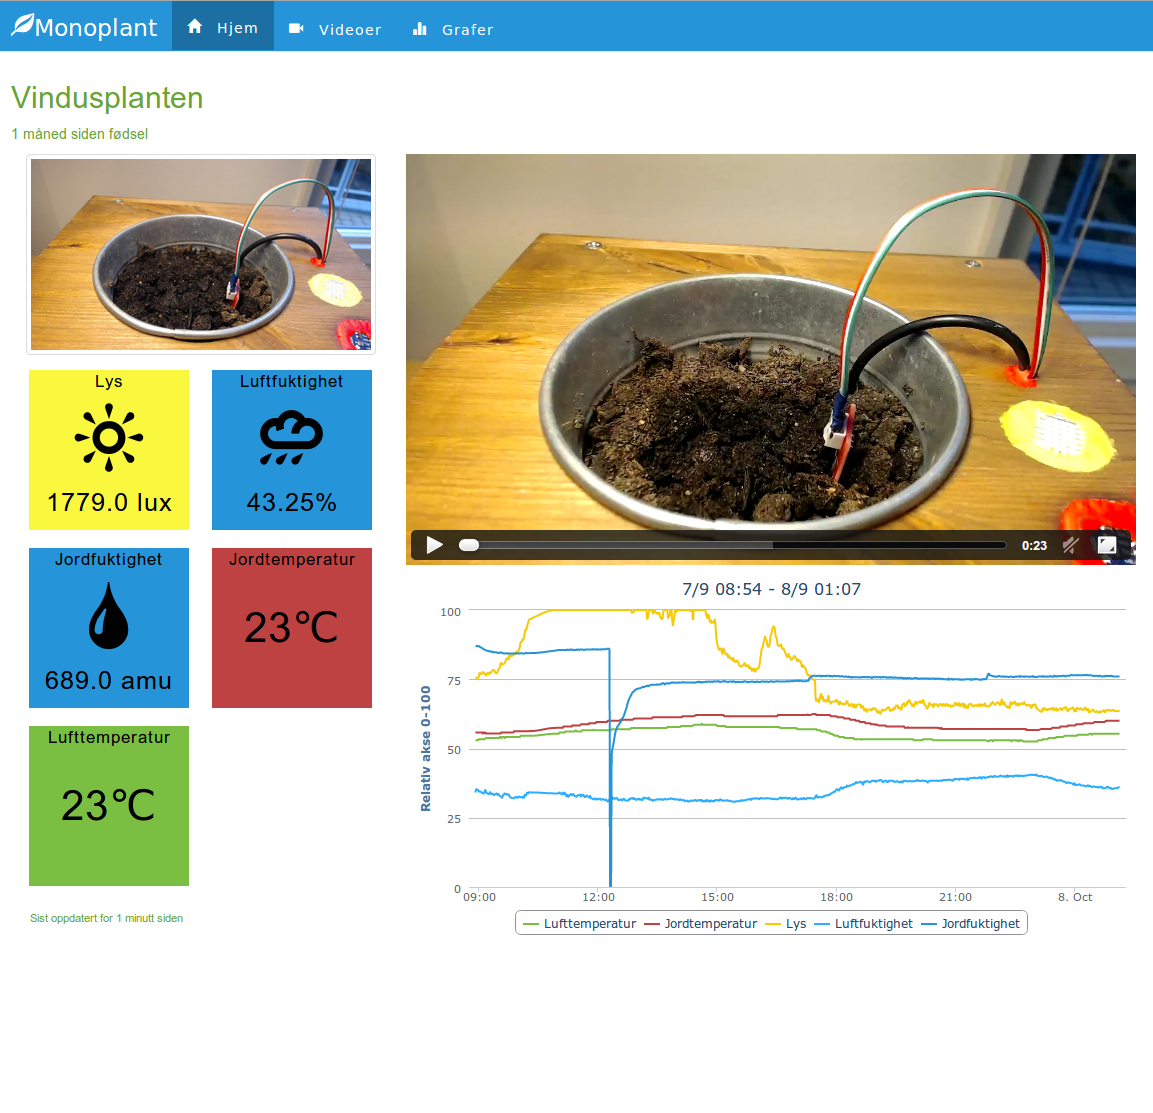
\includegraphics[width=1\textwidth]{img/interface/mainpage.png}
\caption{Screenshot from user interface}
\label{fig:mainpage}
\end{figure}

\subsection{Highcharts}
There are a few serious JavaScript chart libraries available with various types of focus, flexibility and documentation. We ran some tests with Google charts, d3.js and Highcharts, and found that Highcharts provided the most extensive documentation as well as an easy to understand interface. 

The first graph we had to make was a graph containing all the plant data from a given time corresponding to a timelapse video. This meant putting temperature, light, humidity and soil moisture in the same graph, even though they all have different units. 



\begin{figure}
\centering
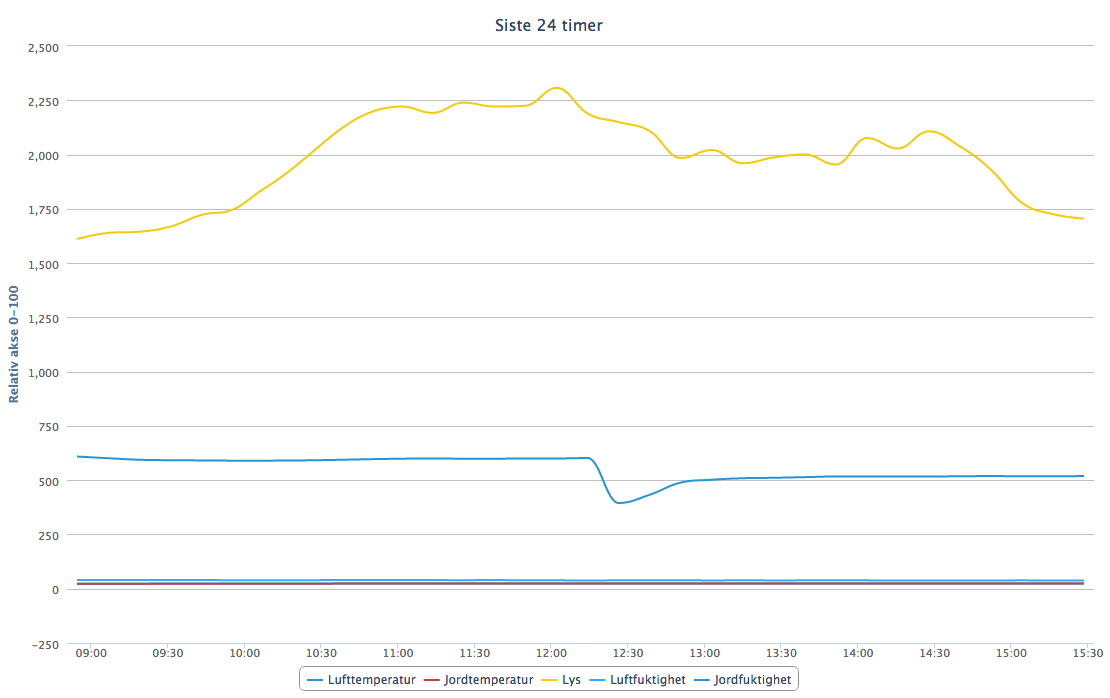
\includegraphics[width=1\textwidth]{img/interface/badgraph.png}
\caption{Screenshot from an unsuccessful graph}
\label{fig:badgraph}
\end{figure}

Our first attempt was done without manipulating the data at all. As Highcharts scales the y-axis based on the element with the highest values, the element with small values appeared as straight lines at the bottom of the graph. In figure~\ref{fig:badgraph} we tried to combine light levels of 2000 lux with temperature levels at $22\,^{\circ}\mathrm{C}$, and as we can see, all the elements except light and humidity are concentrated at the bottom. 

For this graph to display the environmental changes during a day we needed to create a relative scale and map the values to that scale. To exemplify, lets say you have a number \ensuremath{X}, which has a value between \ensuremath{A} and \ensuremath{B}, and you want to map it to a value \ensuremath{Y}, between \ensuremath{C} and \ensuremath{D}. The function is similar to calculating percentage and can then be written as: 
\begin{equation}
Y = \frac{(X-A)}{(B-A)} * (D-C) + C
\end{equation}

%This becomes a slightly more advanced version of calculating percentage (see figure~\ref{fig:mapfunc} on page~\pageref{fig:mapfunc}).

%We chose an output scale from 0 to 100 and wrote a function according to figure~\ref{fig:mapfunc} that mapped the values based on what type of data it was. We set the input scales as can be seen in figure~\ref{fig:mapscale}.

\begin{figure}
	\begin{lstlisting}[style=htmlcssjs]
{
	humidity: { min: 10, max:100 },
	soil temperature: { min:15, max:30 },
	light: { min: 400, max:2500 },
	air temprature: { min: 15, max: 30 },
	soil Moisture: { min: 0, max: 700 }
}
	\end{lstlisting}
	\caption{Mapping scales}
	\label{fig:mapscale}
\end{figure}

Through trial and error, we chose the \ensuremath{C} and \ensuremath{D} values of each unit (see fig.~\ref{fig:mapscale}). Then, after running the data through our new function all the units became visible (see fig.~\ref{fig:goodgraph} on page~\pageref{fig:goodgraph}). As we have mapped all the units to relative units, information of the values at the specific data points is lost. But as the graph is displayed along with the video, we wanted to keep the information level low.  

\begin{figure}
\centering
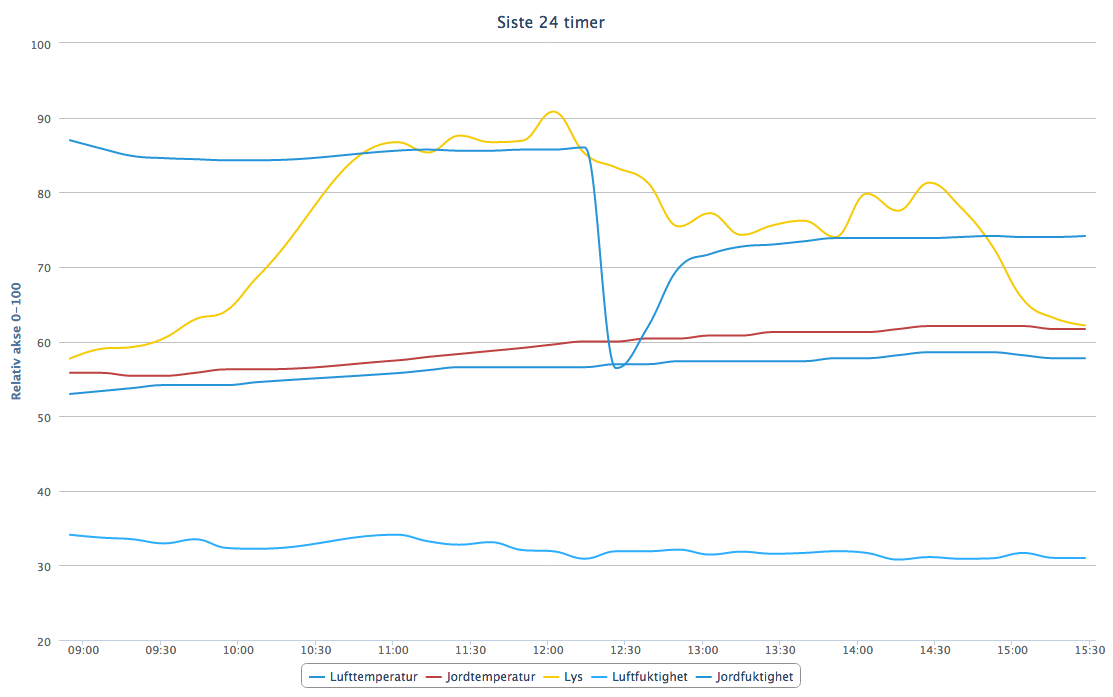
\includegraphics[width=1\textwidth]{img/interface/goodgraph.png}
\caption{Screenshot from a successful graph}
\label{fig:goodgraph}
\end{figure}

%To make sure one can read the appropriate sensorvalues we provide several other graphs, one for the last 24 hours, very similar to the video graph. The only difference is that we have included a mouse-over interaction technique with a tool-tip that displays the actual values alongside the corresponding image of the plant \citep[p.254]{kluge2010simulation}.

Apart from the video-graph and the last 24 hour-graph we provide singular line graphs for each variable. This gives us the ability to display graphs with correct y-axes. 
%The user can select time period for these graphs by interacting with the small graph on the bottom. 

\subsection{Connecting video and graph}
%explain objective
In order to present how changes in sensor variables manifested themselves physically in the plant, we wanted to connect the graph and the timelapse video. The visual solution became to present the video above the graph, both contained within the screen. As the video is playing, a vertical line layered above the graph moves from left to right representing the current point in the video. 

The HTML5 video-element can be accessed through JavaScript, and by checking the state of the video we are able to make the Highcharts graph follow the video based on the \verb@currentTime@ of the videoelement.

\begin{figure}
	\begin{lstlisting}[style=htmlcssjs]
function startVideo(){
	 interval = setInterval(function() {
		 var curtime = video.currentTime.toFixed(2);
		 if(curtime!= lastcurtime){
	 lastcurtime = curtime;
	 curmarker = Math.round(curtime*30);
	 stepTooltip(curmarker);
		 }
	 }, 33);
}

function stopVideo(){
	clearInterval(interval);
}
	\end{lstlisting}
	\caption{Video and graph connection code, written in JavaScript}
	\label{fig:videocode}
\end{figure}

By binding \verb@startVideo()@ to the play-event of the video-element and \verb@stopVideo()@ to the pause and stop event, we are able to move the graph marker as the video plays. The video-element has a built-in event called \verb@timeupdate@, which is triggered when the video's time is changed. However, in practice this event only appeared 3-7 times per second, giving a lagging experience of the graph marker. To overcome this we made a custom function using \verb@setInterval@, which turned out to be a lot faster and more reliable, providing a smooth flow of the graph marker. 


%The reason for using \emph{setInterval} instead of the videos built-in event \emph{timeupdate} is that it is not specified how often the event will fire, but by testing we found that it was somewhere between 3-7 times per second, varying randomly from second to second. This was not often enough as the video had a framerate of 30 frames per second, which meant updating the graph at 1/10 of the speed of the video, resulting in a laggish experience of the graph. We experienced that using \emph{setInterval} gave use much more accuracy when setting it to run every 33th millisecond. No browsers guarantee that the performance of \emph{setInterval} will be faster than 50 ms, but by running tests \citep{adequatleyqood}, we found that the Chrome browser ran this on an average of 4.5 ms. Even though this can be slower when considering the load on the browser when playing a video, we found that in practice most browsers were able to play the video and update the graph simultaneously. 

%!TEX root = ../document.tex
\chapter{Theoretical perspective \& concepts for analysis}

In this chapter we will lay forth the theoretical perspective and theoretical concepts we will apply in this thesis. First we will introduce the \emph{sociocultural perspective} and highlight some key points including \emph{institutional practices}, \emph{zone of proximal development} and \emph{scaffolding}. Further we will look at \emph{multiple external representations} and lastly the concept and method of \emph{Inquiry learning}.

\section{Sociocultural perspective}

%The sociocultural perspective may be thought of as the synthesis of the behavioristic thesis and cognitive antithesis. The behavioristic model focuses on the role of the individual and the notion that knowledge arises through individual drill and practice. In contrast, the cognitive model focuses on the environment and the notion that the environment provides raw material for testing innately conceived hypotheses, thus focusing on instruction methods and acquisitional models. The sociocultural perspective considers the individual in the context of their environment, with a focus on means of mediation between the two. Thus, action is the primary unit in sociocultural analysis, which will be elaborated further in the following paragraphs. 

%The sociocultural perspective considers the individual in the context of their environment, with a focus on means of mediation between the two. Thus, action is the primary unit in sociocultural analysis, which will be elaborated further in the following paragraphs. 


In a biological sense the human species has not evolved significantly the last ten thousand years or so. In fact, changes in our gene pool are only minor, and can’t explain the difference between modern people and people of the Stone Age. Still we are able to achieve tasks that would have been impossible for our ancestors \citep{saljo2001laering}.

The explanation of this discrepancy from a sociocultural perspective becomes evident when one takes into account the \emph{tools} and \emph{signs} we use to mediate the world. We have created a culture where each of the \emph{tools} and \emph{signs} we use has a long history embedded in them. For instance if you are given the multiplication problem 122\texttimes284, you can flip up a calculator and get the answer instantaneously. Similarly, if you were to solve the multiplication problem 7\texttimes4 you can look up in a multiplication table and find the answer easily. These \emph{cultural tools} (calculator and multiplication table) enable you to make sense of the world in a different way than our ancestors. 

From the example given above we can see that there is an “irreducible tension” between the agent and the cultural tool \citep{wertsch1998mind}. Without the multiplication table you would not be able to solve the problem. But the multiplication table is not enough, as it would have been useless without a skilled user. The goal of a sociocultural approach is therefore to: 

\begin{quote}
"Create an account of human mental processes that recognizes the essential relationship between these processes and their cultural, historical, and institutional setting."\citep{wertsch1998mind} 
\end{quote}

This means that the unit of analysis is human action, and how it is mediated by cultural tools, or “agent-acting-with-mediational-means” \citep[\citealp{wertsch1993sociocultural} cited in][]{wertsch1998mind}. The mediated action can never be understood by the properties of only the agent, the mediational means, or the cultural, historical and institutional setting of the mediated activity. An example of this is $\text{H}_2\text{O}$: one can not understand what makes up water if one analyses hydrogen and oxygen separately. The characteristic of the whole is not made up by the characteristics of the elements \citep{vygotskiui1978mind}. Another example is the track-and-field event of pole vaulting. 
\begin{quote}
"The pole by itself does not magically propel vaulters over a cross bar; it must be used skillfully by the agent. At the same time, an agent without a pole or with an inappropriate pole is incapable of participating in the event" \citep{wertsch1998mind}. 
\end{quote}
So while analysis of the elements in isolation may be informative, we will never understand the big picture without taking into account the relation between the mediational means, the agent, and the sociocultural context. 

\subsection{Tools \& Signs}
One important distinction to make when talking about mediated activity is that of tools (physical tools) and signs (psychological tools) \citep{vygotskiui1978mind}. While they are similar in that they can play a mediating role in activity, they are different in the ways they orient human behavior. The tool is externally oriented and must lead to change in physical objects. A basic example of a tool is a hammer. An agent can mediate her activity toward the external world by using the tool to crush a coconut. A sign on the other hand is internally oriented and “changes nothing in the object of psychological operation” \citep{vygotskiui1978mind}. Examples of signs are: diagrams, drawings, language, or as mentioned above, multiplication tables. “It is a means of internal activity aimed at mastering oneself” \citep{vygotskiui1978mind}. 

Another illuminating example of the difference between tools and signs is that of a child presented with a birthday cake. The child does not immediately start eating, but waits until “happy birthday” has been sung and she has blown out the candles. In that sense the cake is a sign as it represents a lot more than just food in the mind of the child. It signifies that she is a year older, that she is going to get presents afterwards, that she is celebrated, etc. On the other hand, from the parents’ point of view, the cake can be used to signify that she is a year older and has new responsibilities in the society. 

If we look at the same example from a behavioristic point of view, another situation emerge. The behavioristic model focuses on the role of the individual and the notion that knowledge arises through individual drill and practice. The girl would therefore know from previous experience that cake tastes good, and immediately start to dig in. 

\emph{In contrast}, the cognitive model focuses on thought processes and the notion that the environment provides raw material for testing innately conceived hypotheses. The reason for the girl not eating the cake would therefore be an internal thought process and the context in which the cake is placed would play a minor role. 

\subsection{Implications for Learning}
“From a sociocultural perspective learning is understood as mastery and appropriation of cultural tools” \citetext{Wertsch, 1998, Säljö, 1999, 2001, cited in \citealp{mifsud2010reconsidering}}. \citet{wertsch1998mind} does however make a distinction between knowing how to use a cultural tool (mastery) and making a cultural tool one’s own (appropriation). Appropriation can be to take the mastery one step further. Oxford dictionary defines it as “the action of taking something for one’s own use”, or as \citet{wertsch1998mind} puts it “making a cultural tool one’s own”. One example of this is a person who has mastered the cultural tool "chords" on a guitar and later appropriates them to a song. It should however be recognized that both mastery and appropriation does not always happen. For example, a person could master the chords on the guitar and perform them flawlessly in class, but dismiss them as terribly ugly at home. Likewise, a person can appropriate chords to a song without mastering the chords themselves.

When we then ask what learning is from a sociocultural perspective, we are also asking “‘which cultural tools are valued?’, and ‘In which contexts do they apply’” \citep{mifsud2010reconsidering}. In order to give an answer to these questions, we have to take into account the cultural, historical and institutional context of the mediated activity. 

To set the scope for our thesis we have decided to place an emphasis on the institutional part of the context, while still acknowledging that the context has cultural and historical aspects.  

\subsection{Social practices}
With a sociocultural perspective on learning, we see external and internal processes as intertwined. By this we try to see student interactions with artefacts and each other as embedded in a cultural, historical and institutional practice, meaning that we take into account the relation between the mediational means, the agent and her contexts. These practices can be embedded into cultural artefacts or as \citet{furberg2009socio} states: "computer based environments can embed such practices in the design". She mentions two types of social practices embedded in Web-based inquiry learning environments: \emph{scientific inquiry} and \emph{institutional practices}.  Scientific inquiry is often expressed by encouraging students to do ideal scientific activities e.g. hypothesis generation, evaluating evidence and constructing explanations. Institutional practices can be expressed in terms of school science as an institutional practice, for example by means of tools that enable the teacher to supervise the students, assignments that makes the students think as if they are beeing assessed, or tools for the students to test their own skills. These practices can also include metaphores taken directly from the institution of school, for example as shown in figure~\ref{fig:scrshotviten} where all the assignments states that you need to be logged in as a student to type in an answer. These "embedded institutional practices can be, and often are, at odds with the ideal practices of scientific inquiry." \citetext{\citealp{chinn2002epistemologically}, referenced in \citealp{furberg2009socio}}

\begin{figure}
\centering
\includegraphics[width=1\textwidth]{img/theoretical/vitenassessment.png}
\caption{Screenshot from viten.no showing student-role metaphor}
\label{fig:scrshotviten}
\end{figure}

Likewise \citet{jimenez2000doing} pose that "doing science" has an obstacle named "doing school". Where "doing science" refers to argumentation or dialog characterized by “construction, representation, evaluation of knowledge claims and investigative methods” \citep{jimenez2000doing}. While "doing school" refers to what actions and activities students and teachers do that instantiates rituals, routines and expectations in educational settings, e.g. review homework assignments, take lecture notes, take tests, complete lab activities etc. \textbf{OBSOBSOBSOBS! DET ER EGENTLIG IKKE JIMINEZ SOM ER PROBLEMET I NESTE SETNING, DET ER DIV ANDRE STUDIER SOM FOKUSERER PÅ DOING SCIENCE OG UTELATER DOING SCHOOL BLABLABLA (SE FURBERGLUDVIKSEN 2008)} \citeauthor{jimenez2000doing} have contributed to the understanding of students argumentation and knowledge claims, but as \citet*{furberg2008students} suggests; a more holistic view is needed to get a rich understanding of the complexity of students' meaning making. Meaning that both the dimension of "doing school" and the dimension of "doing science" needs to be taken into account. 

\subsection{Spontaneous and scientific concepts} \label{cha:spontaneous_scientific}
In the early stages of life, children learn for the most part by experience. Skills such as mastering the native language, walking, running are learned through trial and error. This means that the knowledge of a concept is linked to the concrete experience where she was presented with the concept. A child who is presented with the concept of "brother" by a pointing gesture towards her brother, will at first only associate the word "brother" with that specific person. This is what Vygotsky calls \emph{spontaneous concepts}

An only child on the other hand, will be introduced to the concept of brother through other concepts. A parent can for instance say that "brothers are boys who have the same parents". The concept of brother will then be a general concept for the child, not linked to any concrete experiences, but to the concepts of "boys" and "parents". This is what Vygotsky calls \emph{scientific concepts}

The major difference between these two types of concepts is that spontaneous concepts are developed outside the conceptual framework and only linked to concrete experiences in the mind of the learner. If we presented the child having a brother with the abstract problem of a "brother's brother" \citep{vygotsky2012thought} he would become confused, as his only knowledge of the concept of brother is with situations with his brother

In contrast, scientific concepts are developed within a conceptual framework. They are immediately given a place within the system of concepts, i.e explained by their relation to other concepts. As a result, the child is consciously aware and able to reflect on the concept \citep{van1998concept}. If we presented the only child with the abstract problem of a "brother's brother", he would most likely be able to solve it because of the concepts relation to other concepts in the mind of the child. 

Another example is how children develop a concept of time. In the early stages of life, a child may think that day and night is analogous to light and darkness. This is the spontaneous concept saturated by experience. It is only later in school he learns the scientific concepts of the earth's rotation and its relation to the sun and the moon, which marks days and years. This information has not been appropriated by experience, as the child has not been to space and experienced it, the information is constructed using different signs linked together by the instructor. 

\begin{figure}
\centering
\includegraphics[width=0.6\textwidth]{img/theoretical/conceptpyramid.png}
\caption{The concept pyramid}
\label{fig:conceptpyramid}
\end{figure}

The relationship between these two categories can be explained as an upside-down pyramid. On the top we have the scientific concepts, which are general and abstract. And on the bottom we have the spontaneous concepts, which are specific and concrete. The concepts then move towards each other. The scientific concepts move downwards "toward greater concreteness" in a deductive manner, whereas the spontaneous concepts move "upward toward greater abstractness" \citep{vygotsky2012thought} in a inductive manner.

Even though the concepts move in opposite directions, there is a mutual dependency between them. In Vygotski{\u\i}'s terms: "In working its slow way upwards, an everyday concept clears a path for a scientific concept and its downward development". This means that "the development of a spontaneous concept must have reached a certain level for the child to be able to absorb a related scientific concept" \citep{vygotsky2012thought}. It is therefore essential for the teacher to bring the spontaneous concepts up to a level that makes the scientific concept within reach for the student. By doing this, the student will have the experience, and the related concepts necessary for constructing knowledge of an abstract concept. 

This brings us further to the zone of proximal development, as students who lack consciousness and control over the spontaneous concepts can "find this control within the zone of proximal development" \citep{vygotsky2012thought}.

\subsection{Zone of Proximal Development}
Lev Vygotski{\u\i}, was concerned with the relationship between learning and development, and argues that the theorists of his time such as Piaget, James and Koffka does not provide an adequate view of this. He finds that learning and development are interrelated, and that this relationship has some specific applications in school-learning. \citep[p. 84]{vygotskiui1978mind} Thus, in order to describe these issues he introduces the concept Zone of Proximal Development (ZPD), and defines it as follows:

\begin{quote}“The distance between the actual developmental level as determined by independent problem solving and the level of "potential development" as determined through problem solving under adult guidance or in collaboration with more capable peers” \citep[p. 86]{vygotskiui1978mind}
\end{quote}

The actual developmental level is in other words determined by looking at what a person can do alone. Vygotski{\u\i} found that this traditional way of determining a person's mental development did not hold in school learning, as it only describes what functions in a person that have already been matured. He therefore introduces a new developmental level, the "potential development", which can describe the functions in a person that are in the process of maturation. The actual development of a person is therefore the end product of developing, while the potential development is the state and process of developing. The ZPD can be used as a tool by teachers and instructors to delineate the immediate future of their students, i.e., their actual development of tomorrow.

Vygotski{\u\i} proposes further that ZPD is an essential feature of learning, which distinguishes learning from development, but at the same time provokes developmental processes that would not be possible without learning. In other words,

\begin{quote}“It awakens a variety of internal developmental processes that are able to operate only when the child is interacting with people  in  his  environment  and  in  cooperation  with his peers.” \citep[p. 90]{vygotskiui1978mind}
\end{quote}

By applying the ZPD to learning-situations, the key takeaway is that the analysis alters the traditional view of knowledge or mastery, and shows that the constructed knowledge provides the basis for further development. A great example of this is the process of mastering native language, which initially is learned as a means of communication between the child and other people. The use of language first happens on a social level, in the interaction with people, and is later developed to internal speech and becomes a means to organize thought, i.e., an internal mental function . Vygotski{\u\i} calls this concept the \textit{duality of learning} \citep{vygotskiui1978mind}. 

Another classic example is that of a child trying to grasp a ball. At first the gesture means nothing to the child, but when the mother realizes that the gesture indicates something, the situation changes dramatically. When she gives him the ball, as a result of the hand gesture, the "grasping movement changes to the act of pointing" \citep{vygotskiui1978mind}. This means that the operation that was initially an external activity is now "reconstructed and begins to occur internally" \citep{vygotskiui1978mind}. Thus, \textit{externalization} precedes \textit{internalization}. 

With this in mind, a teacher can understand what developmental processes is maturing in their students, and from that give adapted challenges, show partial solutions and in general tailor what to say and teach next. From this perspective, development is lagging behind learning, and the challenge for the teacher becomes to teach ahead of development, but at the same time not too far ahead. This leads us to the concept of scaffolding, which can be argued to be a refinement of ZPD. 

\subsection{Scaffolding}
Vygotski{\u\i}'s Zone of Proximal Development is the distance between what a person can do alone and what he can do with help from a More Knowledgeable Other (MKO). What types of help and how the MKO should provide it, has not been a focal point for Vygotski{\u\i}. Although \citeauthor*{wood1976role} does not reference to any Vygotski{\u\i}an literature, the term scaffolding introduced by them in 1976, bears resemblance to the very idea of ZPD. As they put it:

\begin{quote}“Scaffolding consist essentially of the adult ‘controlling’ those elements of the task that are initially beyond the learner’s capacity, thus permitting him to concentrate upon and complete only those elements that are within his range of competence” \citep{wood1976role}
\end{quote}

Thus, scaffolding can be applied by MKOs in order to keep the learning process within the learner’s ZPD. There is a is a nuanced balance for how much guiding is needed and a key point is that a person's ZPD is personal, thus a scaffold should be personally adjusted. An example can be if we were to teach two persons how to take a picture with a professional DSLR camera, one being an old woman (Mary) with little insight in technology, the other a young man (Ryan) who has grown up with technology. It is obvious that the two persons have different cultural backgrounds and taking a picture have different meanings to them, hence the tutoring of them need to be differently tailored. In the following section we will go through the six steps of scaffolding provided by \citet{wood1976role} using this example.

\begin{enumerate}
\item{} \emph{Recruitment} - We need to get the learners attention and interest in the task at hand. In our case this could be to show nice pictures of Mary's grandchildren to make her interested in taking nice pictures of them herself. For Ryan we could show the difference between pictures taken with an iPhone and a DSLR camera to make him understand the value of using a DSLR versus his iPhone.

\item{} \emph{Reduction in degrees of freedom} - The task must be narrowed down in order to provide a clear goal that can be reached. For Mary we can say that her task is to take a photo of her grandson playing in the garden with the use of auto-mode. And for Ryan, the task could be to take a landscape photo of his favorite view for his Facebook cover photo with the camera setting called A for aperture, which lets him control the depth of field - an important setting when photographing landscapes. 

\item{} \emph{Direction maintenance} - The learners must be kept on the path towards the goal, which implies a focus on motivation. Both to maintain progression and to keep a focus on the goal. From this point, scaffolding becomes an improvisation skill and it can be hard to plan ahead because of all the unforeseen things that can happen. Ryan can for example stop focusing on the landscape photo and instead take pictures of a car. While Mary starts looking at the pictures contained on the camera's memory stick. In this case one has to evaluate the goal versus the reduction in degrees of freedom. It might be that Ryan is more interested in taking pictures of cars, and since the main goal is to learn to take photos with a DSLR camera, an adjustment of the end product can be done. In Mary's case however, she might be easily distracted, and just needs someone to tell her to focus on taking pictures of her grandson. These are nuances that can be hard to spot, and requires a tutor with good improvisation skills.

\item{} \emph{Marking critical features} - Marking what the learner has done versus what is expected. This could be to show Mary that in her picture, she has left half her grandson's head out of the picture, and that she should try to capture a photo with the whole face visible. For Ryan it could be to point out that he has a very small depth of field in his photo, putting the trees in the foreground into focus, while leaving the mountains in the background blurred. Examples of correct solutions could be used to demonstrate the discrepancies between what the learner has produced and a correct solution.

\item{} \emph{Frustration control} - Balancing the dependency of the tutor and the independent problem solving. Both Mary and Ryan should be given some space to try taking photos, but we should at the same time be observant of when guiding or telling is needed. We could tell them to have the sun behind them to get the right light conditions, and hold the camera with two hands. The major risk here, is that the learner can become too dependent of the tutor, making it harder for the learner to achieve the goal, i.e. taking a picture alone at a later time.  

\item{}  \emph{Demonstration} - Showing a solution to the task, imitating the learner's earlier attempts and possibly correcting errors, with a hope that the learner will imitate back in a more correct manner. For Mary we could take a picture of her grandson, imitating her position, look for the sun, and then correct the position to get the sun behind us. Or for Ryan we could place the camera on a chair and use a timer to reduce movement in the camera, thereby allowing a slower shutter speed, which again allows a higher aperture, increasing the depth of field, giving focus to both the trees in the foreground and the mountains in the background. This might be supplemented by telling, to provide a context to the tutor's actions.
\end{enumerate}

As presented, some of these steps require planning while others require improvisation. Both the planning and improvisation turns out to be tailored to the specific situation at hand with all the complex contexts the learners bring with them to the situation. The steps can either be carried out manually by a tutor, or be mediated automatically by a computer-based system. \citet{fischer1991critics} presents one implementation of a computer-mediated scaffold where a critiquing system gives the user a "reasoned opinion about a product or action generated by a human". Another example is from \citet{furberg2009socio} where prompts requiring user-input is used to promote student reflection. 

One important thing to note when reviewing the literature on scaffolding by \citet{wood1976role} and ZPD by \citet{vygotskiui1978mind} is that these studies are done on pre-school children. Critics may therefore argue that the concepts are not applicable to adult learning. Our stance is that when learning new concepts, both children and adults are alike. New and unknown concepts are new and unknown both for adults and children, and adults therefore become "as children" when introduced with new learning material. The concepts can therefore be used to analyse learning in all contexts where learning takes place. 

%Even though the six steps provided by \citet{wood1976role} can be considered as a framework for scaffolding, it is still quite complex and demands careful consideration by the teacher or the designers of the computer based scaffold.  

\section{Multiple External Representations}
Multiple external representations (MER) have been used since long before the advent of computers for conveying information. Textbooks and manuals often contain images and illustrations, maps show different information in different ways, and whiteboards are used in addition to speech. With digital technology the possibilities of MER are expanded to include dynamic linking between the representations, and the representations can show dynamic information that is not available in the real world, e.g., showing the flow of oxygen. 

In an effort to identify the features of MER, \citet{ainsworth1999functions} has developed a classification framework. She suggests that MER can serve primarily three different purposes in learning situations:
\begin{itemize}
\item{} \emph{Complementary roles} - Different representations can focus on different aspects of the phenomenon under study, or they can contain different information of the same phenomenon. E.g. a topographic map in addition to a road map. 
\item{} \emph{Constrain interpretation} - One representation can be used to constrain the interpretation of the other. E.g. the text “the fork lies next to the spoon”. It is impossible to tell which side the fork is on, but by presenting an illustration of the example, the representation will constrain the interpretation of the text. 
\item{} \emph{Construct deeper understanding} - MER can be used to “promote abstraction, to encourage generalization and to teach the relation between representations” \citep{ainsworth1999functions}. 
\end{itemize}

The three different roles presented above are also the benefits of using MER. Complementary roles can support students to make up for insufficient knowledge of one representation by using another, constrain interpretation can “support the learners’ reasoning about the less familiar representation” \citet{ainsworth1999functions}, and finally the learners can gain deeper understanding of the domain by translating between representations \citep{van2006supporting}. 

On the other hand, when learners are faced with MER they must also undertake additional tasks as to understand the phenomenon or domain in question. This may lead to a heavy cognitive load, which “may leave less resources for actual learning” \citetext{Sweller, 1988, 1989, referenced in \citealp{van2006supporting}}. A key issue is then to reduce the cost for learners associated with MER, while keeping the benefits. 

\section{Inquiry learning}
According to \citet{prince2006inductive} science has traditionally been taught in a \textit{deductive} manner. In the same way as Sherlock Holmes collects piece by piece to form a theory, the students collect pieces of models and illustrations to grasp a scientific concept. Little attention is paid to why the students should learn the material, apart from having to perform on tests.

On the other hand we have the \textit{inductive} ways of teaching and learning. Instead of beginning with the theory, the students are presented with some sort of task, which becomes the motivation to learn the tools required to solve the task. Examples of this can be to make a battery in a science class, or finding out why potato-chips bags seem more inflated on the top of a mountain than by the sea.

Inquiry learning involves giving the students "questions to be answered, problems to be solved, or a set of observations to be explained" \citep{prince2006inductive}, or in other words: giving the students incentives to ask for information. There are several other inductive learning methods, such as problem-based learning, discovery learning and project-based learning, which all can be explained with the same statements as inquiry learning. Inquiry learning can therefore be seen as an umbrella term for inductive learning methods. \citep{prince2006inductive}

\citeauthor*{staver1987analysis} \citetext{\citeyear{staver1987analysis}, referenced in \citealp{prince2006inductive}} differentiates between \emph{structured inquiry} (e.g. tutorials), \emph{guided inquiry} and \emph{open inquiry}. This relates to the ZPD and scaffolding. Depending on the student's developmental level, different framings of the inquiry process are needed. To scaffold the inquiry learning process is not an easy task. In a review article, \citet{de1998scientific} identify four problems that learners may encounter when engaging with inquiry learning: \textit{hypothesis generation}, \textit{design of experiments}, \textit{interpretation of data}, and \textit{regulation of discovery learning}. They continue to argue for the need of supporting students during the process of scientific inquiry, providing scaffolds for each of these problems. The challenge then becomes "guiding students to the “right” path, but at the
same time letting them discover and make the discovery their own." \citep[p. 247]{kluge2010simulation}. In other words the students need to be steered towards the interesting discoveries, but at the same time have the freedom to explore and not be commanded in any way.

\subsection{Misconceptions}
Misconceptions appear in most educational contexts. According to \citet{gomez2008elementary} students have "qualitative differences in his or her understanding of science that is often inconsistent with what the teacher intended through his or her instruction". These are often deeply rooted, and remain intact even after instruction. This becomes especially relevant when dealing with inductive learning methods, as the students are given more freedom to explore their own ideas, and thus more freedom to pursue tracks that may lead to different conclusions than the ones intended by the instructor.

The term itself has been given many labels in research literature, depending on the focus: "alternative frameworks", "preconceptions", and "student ideas" are just some of them. An important factor here is how misconceptions are perceived. Are they resources for learning, or obstacles that the learner has to overcome? If we look at meaning making from a constructivist point of view, advanced knowledge is built upon prior understanding. Misconceptions then become "faulty extensions of productive prior knowledge" \citep{smith1994misconceptions}.

To then simply write misconceptions off as mistakes is, according to \citet{smith1994misconceptions}, a too narrow view in their role in learning. If we take the example of stating that "multiplication makes numbers larger", it is indeed an accurate explanation of most multiplication pieces. The problem arises in the few cases where we multiply by non-natural numbers. The conception that leads to erroneous conclusions in some contexts can be quite useful in others \citep{smith1994misconceptions}. The misconceptions are therefore for the students "conceptions in their own right with plausibility and at explanatory power" \citetext{Smith, diSessa \& Roschelle 1993, referenced in \citealp{larkin2012misconceptions}}. 

%As stated before, the goal then becomes to scaffold the students in such a way that the interesting discoveries are made, and the misconceptions discussed. 

\section{Summary of Concepts for Analysis}
We have now introduced the Sociocultural perspective and several important concepts within and besides its frames. Further we will use the Sociocultural perspective and the following concepts to guide our research design and discuss our findings:

\begin{itemize}
\item{Zone of Proximal developement (ZPD)}
\item{Scaffolding}
\item{Misconceptions}
\item{Multiple external representations (MER)}
\item{Institutional settings}
\item{Inquiry learning}
\item{Everyday language \& Scientific language}

\end{itemize}
%!TEX root = ../document.tex
\chapter{Empirical settings and methods}
In this chapter, we will present the empirical setting and methods used in this thesis. First we will describe the empirical setting in which the data collection took place. Then we will proceed to present the methods for gathering data with a description of the technicalities of the data. Lastly, we will describe the procedures for selection and analysis of data.

\section{Case Study}
%vet ikke helt hva jeg har starta her, tror jeg må lese noen oppgaver med casestudy.
In our thesis, we have chosen gather data through a qualitative case study.  One of the most important reasons for choosing a case study was as \citet{yin2003case} states: "you want to cover contextual conditions because you believe they are relevant to the phenomenon under study". As the case was students inquiry about photosynthesis, it could not be examined without the context, the school, or more precisely the biology classroom setting where Monoplant was inserted. 



\section{Empirical setting}
The collection of data material used in this thesis took part in late autumn 2013, at a high school located in the center of Oslo. The school has a high threshold for admission, with a lower requirement of 43.5 points out of 60 in 2010 \citep{utdanningsetaten}. Thus, the students at this school are (mostly) high achievers. 

Contact with the school was first initiated through Intermedia, and a presentational flier was sent as an explanation of the project (see chapter \ref{samtykkeskjema}). A teacher contacted us, and luckily our request coincided perfectly with a two-week time frame for reviewing photosynthesis in his biology class. The teacher was therefore willing to test out our application instead of performing one of the experiments described in the textbook. 

The class selected was a biology class at the highest level offered at the school, biology 2, which has an extensive curriculum covering e.g. photosynthesis, enzymes and energy transmitters \citep{bios}. The class consisted of 11 girls and three boys between 17 and 18 years of age (vg3). For the main part of our data collection, all of the students were present. All of them agreed to participate in the study, but due to technical limitations and a busy time schedule, the primary data collection was  done with a small sample of the group. 

\subsection{Ethics}
Prior to the data collection, an application was sent to NSD (Norwegian Social Science Data Services) requesting permission to film the students. The application was approved with only minor changes to how the material was to be treated after completion. In addition all the students taking the class were given an consent form stating that participation was voluntary, and all material would be kept anonymous (see appendix). 

Throughout this thesis, and in the transcripts of video data, all the students' names have been replaced by pseudonyms and the name of the school is never mentioned. The data material containing identifying information of the students has been and will be stored securely on a separate hard drive at Intermedia, and will be deleted  upon termination of the project. 

During our time at the school we were always open about our role as researchers, and explained on several occasions how the data was going to be used. 

\subsection{Planning the experiments}
An initial planning and presentational meeting was held on the 21st. of October with the teacher. A thorough presentation and demonstration of the system was given, along with a discussion of the functionalities of the system, to see if it would spark some ideas for experiments. 

Stressing the importance of a scientific method, the teacher suggested that we could conduct two experiments, using the different sensors in the system to change one variable, while keeping the others relatively controlled. We agreed that the factor that would be easiest to control, yet yield interesting results was light intensity and light quality (wavelength). The first experiment would involve keeping the plant located in a window facing west, receiving sunlight and light from the fluorescent indoor-lighting, while we in the second experiment would relocate the plant to a light proof cabinet where it would only receive light of a known wavelength. Each of the two experiments would span a one-week period, depending on the time needed for measurable results.

\subsection{The experiments}
The project was presented for the class during a one-hour lecture on Friday 25th of October. We used the opportunity to give an in-depth explanation and demonstration of Monoplant, as well as explaining how we would collect and use the data material gathered. We then proceeded to initiate the first experiment, which went on for seven days until Friday 1st of November when the second experiment was initiated. The second experiment went on for 13 days until Wednesday 13th of November when the primary data collection session took place. During the experiments we as observers and researchers were present at four separate occasions, observing what the teacher was focusing on, and the nature of the class discussions. In addition we answered any questions they had regarding the system, and observed how it was used by the teacher and how the students interacted with it. 

\begin{figure}
\centering
\includegraphics[width=0.8\textwidth]{img/empiricalsetting/window.jpg}
\caption{The experimental setup located in the window}
\label{fig:windowplant}
\end{figure}

\begin{figure}
\centering
\includegraphics[width=0.8\textwidth]{img/empiricalsetting/windowsystem.jpg}
\caption{The plant receiving natural light}
\label{fig:windowsystemplant}
\end{figure}

\subsubsection*{The plant in the window}
The first experiment was conducted with a setup in the window as shown in figure~\ref{fig:windowplant}. The system was located in the front of the classroom near a door leading to the adjacent classroom, visible and in reach of everyone walking by. As figure~\ref{fig:windowsystemplant} shows, there is between 50 and 70 seeds in the pot. The plant was located in the window sill, exposed to sunlight or daylight depending on the weather, in addition to the fluorescent indoor-lighting. Due to the time of year, and lack of people using the classroom in the evening, this meant that the plant would get light in the period between 08:00 and 17:00.

It turned out that the system was draining power from a power outlet that was either connected to the indoor light or timer based, as the system went down and did not post data between 19:00 and 07:00. We also had some technical issues with the system from 25th of October to 27th of October, resulting in lost data from the first seeds germinating.

\begin{figure}
\centering
\includegraphics[width=0.8\textwidth]{img/empiricalsetting/cupboard.jpg}
\caption{The system located in the cabinet}
\label{fig:cabinetplant}
\end{figure}

\begin{figure}
\centering
\includegraphics[width=0.8\textwidth]{img/empiricalsetting/cupboardsystem.jpg}
\caption{The plant in the cabinet, receiving green light}
\label{fig:cabinetsystemplant}
\end{figure}

\subsubsection*{The plant in the cabinet}
The second experiment was conducted with a setup in a cabinet as shown in figure~\ref{fig:cabinetplant}. The cabinet was located in a corner in the front of the classroom behind the teacher's desk, hidden and not nearly as accessible as the plant in the window. The picture in figure~\ref{fig:cabinetplant} is taken with light from the room coming in to the cabinet, hence it does not reflect the lighting conditions in the cabinet during the experiment. The cabinet door was closed and the lamp above the plant was emitting green light 24 hours a day, hence figure~\ref{fig:cabinetsystemplant} shows the lighting conditions more correctly. It is also worth noting that the pot contains around 30-40 seeds more than in the first experiment. When this experiment took place we did not have any technical issues, the system posted data continuously for the whole period.


\section{Methods}
Different methods for data collection was discussed and reviewed early on in the project. Our most influential source, regarding paradigm, methodology and method was the tradition for using qualitative data in information systems research in the design group at department of informatics. As our primary data source we chose video data with the use of multiple cameras and a screen dump. This was collected during a 45-minute session after the completion of the experiments, resulting in 3x45 minutes of video data and 45 minutes of audio data. Supplementary data from this session includes the written answers from the groups that were not filmed, and our personal notes. In the following sections the methods used will be discussed. 

\subsection{Video and audio}
It was determined early in the project that video and audio recording were to be used. The primary reason for this was the tradition at Intermedia, as video data collection has been used and thoroughly tested by a number of researchers here. This meant that we would get a lot of help from co-located researchers in what microphones to use, placement of cameras, operation of the equipment, etc. 

A total of 45 minutes of video and audio was recorded, using three separate video sources, and three microphones. One camera was placed in front of the group, able to capture facial expressions and where the students were looking. This camera had an external microphone connected that we placed on the table in front of the students, allowing us to filter out some of the noise in the classroom. The second camera was placed behind the students on their right hand side, facing the computer screen. This camera's primary function was to capture where the students were pointing and what they were doing on the laptop. The audio source of the second camera was the built-in microphone, which proved to cover most of the audio in the classroom. In addition to the video cameras we recorded a screen capture from the laptop, showing exactly what the students were doing in the system. The laptop had a built-in microphone as well but we only used the sound from camera two and the laptop to synchronize the different videos.
\begin{figure}
\centering
\includegraphics[width=0.8\textwidth]{img/empiricalsetting/class_diagram.png}
\caption{Camera setup}
\label{fig:camerasetup}
\end{figure}

\subsection{Passive observation}
During the experiments we were present at four separate occasions. The primary reason was to ensure that the system was working, assist with any technical difficulties regarding the user interface, and to ensure a smooth operation of the experiments. But we would also take notes regarding how the system was used in the lecture, if or how students showed interest in the experiments, and how the teacher was conveying information about photosynthesis in general. While these observation sessions were not thoroughly planned, and the data material never systematized, it proved to be a good supplementary data source to help us structure and make sense of our primary data. We would later on also use these notes as discussion points and indexical resources when reviewing the data material. 

\subsection{Student produced material}
While we filmed the group of students selected for our main data gathering, the rest of the class was divided into groups and told to discuss and write down answers to the given assignments. These answers were handed in and rewritten into computer documents later (see appendix X). This became a fine supplemental data source, as it gave an insight of what answers fellow students of the class came up with in a less monitored setting. 

\subsection{Web logs}
In order to review activity on the web page (\url{http://Monoplant.me}), Google Analytics tracking system was installed. Although we did not use this extensively, it allowed us to see if and how often the system was used, and if students were using it at home or only during classroom hours. 

\section{Analytical Procedures}
From mid November till late December 2013, we were observing, listening, transcribing and discussing the material. In this section we will discuss how we approached, selected and made sense of the data once it was collected.



\subsection{Approaching the data}
\citet{derry2010conducting} speaks about two different approaches to select parts of a video corpus for further examination: the \emph{inductive} and the \emph{deductive} approach. Inductive approaches apply when a minimally edited video corpus is collected and investigated with broad questions in mind but without a strong orienting theory. Deductive approaches involve identifying or creating a suitable video corpus and systematically sampling from it to examine specific re-search questions. \citep{derry2010conducting} To start with, we clearly fit into the inductive approach, but as many researchers have experienced: once you find something, you start looking for it. Hence our approach became leaned more to the deductive side later in our analysis.

To make sense of the data gathered we looked at it in several different ways with different focuses. Below is a chronological list of the ways we approached the data. 

\begin{enumerate}
\item{Initial screening of main video corpus, locating interesting interaction}
\item{Transcription of main video corpus}
\item{Watching supplemental video material to make detailed notes on interactions with the system}
\item{Watching the main video corpus with our supervisor and discussing which events and interactions are interesting and/or can be explained by existing theory}
\item{Select parts of transcript that are of interest}
\item{Detailed transcriptions of these parts}
\item{Writing explanations for these interactions}
\item{Linking interactions to support each other}
\item{Cut excerpts that did not fit together with other excerpts}
\item{Linking chunks of interactions to related theory}
\end{enumerate}

While we still had the impressions from the data collection fresh in mind, we sat down and watched all the video material. During the screening process we tried to make a content-log to get a better overview of a large corpus of data and select cue points in the video where interesting interaction took place, focusing on change in context and contradictions. This was followed by a rough transcription, using mostly audio and video from the camera facing the students. At this point we focused mostly on transcribing what was said, not paying attention to small audible details such as intonation. 

We then went on to the third step in the process, bringing in additional video material to generate thick descriptions of the interesting interactions taking place. Using audio cues, we merged all the three video files into one, so that the screen was divided into three parts: one for the camera facing the students, one for the camera facing the screen, and one for the screen dump. This enabled us to make a more detailed transcript of the parts containing inaudible utterances.

At this point in the process we presented the transcript and screened the video along with our supervisor, marking the points in the video that we deemed most interesting. In the following discussion a list of themes or grouping categories was selected, which would be subject to further analysis. A selection of excerpts from the transcripts was then picked out for further analysis where we kept focus on intonation, gestures, etc. to provide a thorough description of the events unfolding. 

As shown in the list, our approach was quite open to begin with, scanning the complete video corpus for what we found interesting. Once we began to find parts that interested us, we started to look for similar events and contradicting events. With help from our supervisor we found theoretical concepts we could link to our material, which again gave us an incentive to look for a specific type of material.

\subsection{Interaction analysis}
%Crang & cook: Video recordings can be criticized by pointing out that it is the researcher that selects the frame and focus. Hence the data can become biased. However, by trying to frame interaction generically, and providing a video, getting other people to double check coding and transcription.
The analytical procedure employed within this thesis is \emph{Interaction analysis} \citep{jordan1995interaction}, which emerged from fields such as ethnography, sociolinguistics, ethnomethodology, conversation analysis, and sociocultural theories. \citeauthor{jordan1995interaction} describes it as follows:

\begin{quote}
An interdisciplinary method for the empirical investigation of the interaction of human
beings with each other and with objects in their environment. It investigates human
activities such as talk, nonverbal interaction, and the use of artifacts and technologies,
identifying routine practices and problems and the resources for their solution \citep[p39]{jordan1995interaction}
\end{quote}

For Interaction analysis to become a reality video and audio recording technology has been a vital resource. The combination of recording talk as well as nonverbal interaction and the ability to replay a sequence as many times as necessary gives us the possibility to analyze more thoroughly. Combining this micro-level data of interaction with ethnographic data gives us a means of analyzing how the interaction is part of the situated context and institutional practices. \citep{furberg2009scientific}. 

\subsection{Systemic vs. dialogic}
\citet{arnseth2006approaching} introduces a distinction between two approaches to CSCL research: \emph{systemic} and \emph{dialogic}. A main feature of studies characterized to be using a \emph{systemic approach}, is that they generate models of how features of the technological system reviewed affects reasoning, collaboration, structures of discourse etc. The analytical focus is on describing the systematic relations between forms of social interaction, and specific types of support or other contextual factors on the one hand, and qualities of outcome on the other. \citep{arnseth2006approaching} In other words, \emph{systemic} studies tend to measure how much a specific feature or configuration in a CSCL-tool affects learning outcomes in terms of "measurable" or "quantifiable" variables. The result of this analytical practice is often a formulation of a model or reformulation of an existing model, which may state that a CSCL application together with a certain practice, are likely to produce a positive learning outcome.

\citeauthor*{arnseth2006approaching} argue that there has been little interest in the emergent characteristics of actions that take place when CSCL-tools are introduced in schools. As they write: \emph{"we need to examine more closely how the meaning and functions of CSCL applications are actually constituted in practice."} \citep[p. 181]{arnseth2006approaching}. Hence they introduce the \emph{dialogic} approach, where CSCL applications are not treated as a variable with features and configurations that in relation to other variables i.e. learning outcome can be determined statistically. Instead, the analytical concern  of the \emph{dialogic} approach is with how computer applications provide a new context for social interaction.

%\sout{ By observing the class during our visits to the school during the experiments, and by reading the textbook chapter on photosynthesis, we gathered ethnographic data on how the class worked together and what they were expected to know about photosynthesis. }

%\sout{Even though we have done a case study in a real educational setting, considering these ethnographic data is important if we are to keep a dialogic perspective.}


%\sout{At point 8 in the list, we had found over 20 excerpts that we wanted to present and discuss. By categorizing these into four themes: \emph{Hypothesis generation and testing}, \emph{Misconception}, \emph{Conceptualization} and \emph{Linking between representations}, we were able to find the best excerpts to represent the themes. Hence we ended up with 11 excerpts, which will be presented in the following chapter.}

%!TEX root = ../document.tex
\chapter{Data \& Analysis}
In this chapter we will present the findings from our case study with a focus on themes relevant to our research questions. Each of the themes contain at least one Excerpt with a context description, excerpt from the transcript, and an analysis of the unfolding events. 

The first theme (\ref{cha:hypothesisgeneration}) is named \textit{Hypothesis generation and testing}. Here we follow a hypothesis from generation to falsification to a new improved hypothesis. Then we move on to \textit{Misconception} (\ref{cha:guidedinquiry}) where we show examples of how misconceptions can be addressed successfully or unsuccessfully by the teacher, and how it can lead to hypothesis generation based on false premises. The third theme (\ref{cha:conceptualization}) is dubbed \textit{conceptualization} and presents three Excerpts regarding scientific and everyday language. The last theme (\ref{cha:linking}), \textit{linking between representations}, aims to show how the students relate the digital representation to the physical world (biology of plant).  

For the sake of simplicity the first experiment, where the plant was located in the window has been named plant A, and the second experiment where the plant was located in the cabinet, plant B. 


\begin{table}[H]
\begin{center}
	\begin{tabular}{l r r } \toprule
	Who &  Interactions  & Percentage\\ \midrule  
	Linda &	 14  & 3.67\% \\
	Nora&	118 & 30,97\% \\ 
	Siri& 	182 & 47.77\% \\
	Fredrik& 67 & 17.59\% \\ \midrule
	All &	381 & 100\%\\
	\bottomrule
	\end{tabular}
\end{center}
\caption{Verbal interactions by participant}
\end{table}

\section{Hypothesis generation and testing}
\label{cha:hypothesisgeneration}
\subsection{First claim}
\subsubsection*{Context}
\label{firsthypothesis}
We enter the situation at the beginning of class. The students have been divided into groups, and they are approximately two minutes into the task. Preceding this discussion, the students have tried for about one minute to figure out what the task is about, and what the two experiments involved. Siri has read out loud the first question in the assignment: "what did you expect would happen?" (in the experiment), and they have rehearsed some of the theories presented in previous lectures (e.g soil moisture decreasing over time). Prior to the excerpt, the students have appeared a bit insecure about the task. But as we enter the setting they seem more focused and interested, and the discussion has changed from making general observations to generating hypotheses.

\subsubsection*{Excerpt 1}
\begin{table}[H]
	\begin{center}
		\begin{tabular}{r l p{7cm} p{3cm} } \toprule
				Time &  Who &  Speech  & Action \\ \midrule 

			2:04 %time
			&Nora %name
			&\parbox[t]{7cm}{\raggedright hehe.. mm.. hmhm .. når den stod i skapet så.. jeg visste ... %speech 
			}&\parbox[t]{3cm}{\raggedright  %action 
			}
			\\

			2:13 %time
			&Siri %name
			&\parbox[t]{7cm}{\raggedright ... neddi skapet ... %speech 
			}&\parbox[t]{3cm}{\raggedright  %action 
			}
			\\

			2:13 %time
			&Nora %name
			&\parbox[t]{7cm}{\raggedright eller jeg visste ikke helt hva den skull.. hva som skulle skje da egentlig .. %speech 
			}&\parbox[t]{3cm}{\raggedright  %action 
			}
			\\
			2:16 %time
			&Siri %name
			&\parbox[t]{7cm}{\raggedright .. det var det planten stod i skapet også skulle det være bare grønt lys på den ... men det kan jo hende for eksempel at det kom litt annet lys inn i skapet også .. så da er det ikke sikkert at det bare var grønt lys ..  %speech 
			}&\parbox[t]{3cm}{\raggedright peker på skapet %action 
			}
			\\

			2:31 %time
			&Nora %name
			&\parbox[t]{7cm}{\raggedright  %speech 
			}&\parbox[t]{3cm}{\raggedright nikker %action 
			} 
			\\

			2:31 %time
			&Siri %name
			&\parbox[t]{7cm}{\raggedright og planten tar jo opp littegrann grønt lys også, men ikke så mye .. så derfor kunne det hende atte den ikke vokste like my.. eller jeg trodde at den ikke ville vokse like mye i skapet .. siden da fikk den bare grønt lys ...  %speech 
			}&\parbox[t]{3cm}{\raggedright  %action 
			}
			\\
			2:46 %time
			&Nora %name
			&\parbox[t]{7cm}{\raggedright ... mmm ... %speech 
			}&\parbox[t]{3cm}{\raggedright  nikker%action 
			}
			\\
		\end{tabular}
	\end{center}
	\caption{First hypothesis}
	\label{excerpt:hypothesisgeneration}
\end{table}

\subsubsection*{Analysis}
\begin{figure}
\centering
\includegraphics[width=\textwidth]{img/dataandanalasys/absorbtion.png}
\caption{Absorption of wavelengths by pigments \citep{bios}}
\label{fig:absorption}
\end{figure}
At first, Nora is not sure what would happen to the plant given green light in the cabinet (plant B). Siri, as one who thinks out loud, promptly starts reflecting on what could have happened. First she proposes that the plant was given more than green light, indicating that there could be error sources to the experiment. This is acknowledged by a slight nod from Nora. Then she goes on to reflect on the wavelengths plants absorb, agreeing that they only absorb a small amount of green light. They conclude that the plant in the cabinet would not grow as much as plant A. Nora agrees with this hypothesis by nodding and saying "mmm". 

The basis for the statement that plants only absorb a small amount of green light can be found in the textbook: "reflected and transmitted light can hit our eyes and give the object color" \citep[pg. 103]{bios}. The book also contains a graph of the different pigments according to the wavelengths of light they absorb (see fig. \ref{fig:absorption}), clearly showing that chlorophyll absorbs little of green light. In addition, the teacher has used this as a discussion point in earlier lectures, asking why plants' leaves appear green. 

\subsection{Claim refuted}

\subsubsection*{Context}
We enter the setting immediately after the excerpt explained in the previous section. Siri has generated a hypothesis, that she wants to test out. The mood in the group has now gone from laughter and insecurity about the task to concentration and goal-driven work. The overall noise level in the class room has also fallen significantly. 

\subsubsection*{Excerpt 2}
\begin{table}[H]
	\begin{center}
		\begin{tabular}{r l p{7cm} p{3cm} } \toprule
			Time &  Who &  Speech  & Action \\ \midrule 

			2:47 %time
			&Siri %name
			&\parbox[t]{7cm}{\raggedright ...eller nesten bare grønt lys ihvertfall ... men hvor mye vokste den egentlig? er det den ((refererer til planten på bordet)) som stod i skapet? %speech 
			}&\parbox[t]{3cm}{\raggedright peker på planten som står på pulten %action 
			}\\

			2:52 %time
			&Sjur %name
			&\parbox[t]{7cm}{\raggedright ja %speech 
			}&\parbox[t]{3cm}{\raggedright  %action 
			}\\

			2:53 %time
			&Nora %name
			&\parbox[t]{7cm}{\raggedright OJ(!) %speech 
			}&\parbox[t]{3cm}{\raggedright  %action 
			}\\

			2:53 %time
			&Siri %name
			&\parbox[t]{7cm}{\raggedright Den har jo vokst ganske mye %speech 
			}&\parbox[t]{3cm}{\raggedright smiler %action 
			}\\
			2:59 %time
			&Siri %name
			&\parbox[t]{7cm}{\raggedright men var stilkene på den som stod i vinduet var de også hvite? %speech 
			}&\parbox[t]{3cm}{\raggedright Peker mot vinduet %action 
			}\\
		\end{tabular}
	\end{center}
	\caption{Claim refuted}
	\label{excerpt:testinghypothesis}
\end{table}
\subsubsection*{Analysis}
After Siri proposed that plant B would not grow as much as plant A, she wants to find out if it holds. Suddenly she notices the plant, which is placed on the table in front of them, and exclaims, "is it that one(!)?". When Sjur confirms, the whole group and especially Siri look surprised. It seems like they all firmly believed that the hypothesis Siri presented earlier (see section \ref{firsthypothesis}) should hold true. Their knowledge of photosynthesis would also point to the plant not growing as much as it had. Thus, the first hypothesis generated by the group has now been falsified. 

As a reaction to this Siri stops to think for a few seconds before she points at the window and asks: "were the stems on the one in the window also white?". This is a very appropriate scientific question, as a plant with absolutely no photosynthesis would most likely be white, as a result of having no pigments. The reason for her asking this may be related to a comment made by another student in a previous lecture. He had observed that when they put plants in the basement for winter storage, the leaves would turn white. 

\subsection{A new claim}
\subsubsection*{Context}
This next excerpt is from a situation occurring only a few seconds later. The group has been instructed to interact with the system on the computer in front of them to find the answer to the question asked at 2:59 \emph{"were the stems on the one in the window also white?"}. When we enter the situation they have a video of plant A on the screen in front of them, dated 31st of October, ready to play. 

\subsubsection*{Excerpt 3}
\begin{table}[H]
		\begin{center}
			\begin{tabular}{r l p{7cm} p{3cm} } \toprule
					Time &  Who &  Speech  & Action \\ \midrule 
				3:21 %time
				&Nora %name
				&\parbox[t]{7cm}{\raggedright Ja for karse har jo hvit stilk %speech 
				}&\parbox[t]{3cm}{\raggedright  %action 
				}\\

				3:23 %time
				&Siri %name
				&\parbox[t]{7cm}{\raggedright Ja det de har hvit stilk de også %speech 
				}&\parbox[t]{3cm}{\raggedright  %action 
				}\\

				3:24 %time
				&Fredrik %name
				&\parbox[t]{7cm}{\raggedright mhm ... mmja så da er det jo egentlig ganske ... ja ikke så stor forskjell da på de som stod ...  i skapet ((peker på planten på border)) og de som stod i vinduskarmen hvis man bare ser på ...  utseende %speech 
				}&\parbox[t]{3cm}{\raggedright Dette sies mens Siri starter videoen, hun stopper også videoen før de har sett den halvferdig. %action 
				}\\

				3:37 %time
				&Siri %name
				&\parbox[t]{7cm}{\raggedright ja .. men da ville jeg kanskje tenke at det kan hende at det kom inn annet lys enn det grønne lyset også. siden de har vokst så bra, og at de vokser bedre hvis de får flere.. lys i flere bølgelengder enn bare grønt lys %speech 
				}&\parbox[t]{3cm}{\raggedright Stemmeleiet går opp mot slutten av setningen, og løfter blikket fra arket for å få bekreftelse
				 %action 
				}\\
			\end{tabular}
		\end{center}
	\caption{A new claim}
	\label{excerpt:newhypothesis}
\end{table}
\subsubsection*{Analysis}
Here Nora and Siri find that the stem of plant A is white as well. Fredrik then says that there is not much difference between the two plants if they consider just their looks. Since Siri got that answer to her question about the stems, she has ruled out that photosynthesis is not happening to the plant in the cabinet. Thus she formulates a new hypothesis, which presumes an error source in the experiment: the plant has grown as much as it did because light of other wavelengths than green has entered the cabinet.
This hypothesis would also explain why her first hypothesis, that the plant would not grow as much as the other, failed. It is also worth noting that monoplant does not provide a means of observing the wavelength of light, but we did however provide the students with a spectrometer image of the green light as shown in INSERT FIGREF HERE.

\section{Misconception}
\label{cha:guidedinquiry}


\subsection{Assumptions based on a misconception}

\subsubsection*{Context}
Prior to the following excerpt, the students have been looking at the movements of the two plants, and observed that plant A is moving towards the sun, a phenomenon called \emph{heliotropism}. They are now observing the movement of plant B. Fredrik has just pointed out that it is growing straight up without any skewed movement like plant A. As we enter the setting, all the students are concentrated and watching a video of plant B from the 4th of November.


\subsubsection*{Excerpt 4}

\def\arraystretch{1.5}
\begin{table}[H]
	\begin{adjustwidth}{-4em}{-4em}
		\begin{center}
			\begin{tabular}{r l p{7cm} p{3cm} } \toprule
				Time &  Who &  Speech  & Action\\ \midrule  

				7:46 %time
				&Nora %name
				&\parbox[t]{7cm}{\raggedright Jeg føler at de vokser veldig mye inni ... skapet eller er det? ... %speech 
				}&\parbox[t]{3cm}{\raggedright  %action 
				}\\

				7:51 %time
				&Siri %name
				&\parbox[t]{7cm}{\raggedright Ja det virka som om de vokste ... %speech 
				}&\parbox[t]{3cm}{\raggedright  %action 
				}\\

				7:53 %time
				&Nora %name
				&\parbox[t]{7cm}{\raggedright ... ser ut som de ble lenger lissom ... %speech 
				}&\parbox[t]{3cm}{\raggedright  %action 
				}\\

				7:53 %time
				&Siri %name
				&\parbox[t]{7cm}{\raggedright ... enda mer der. %speech 
				}&\parbox[t]{3cm}{\raggedright  %action 
				}\\

				7:54 %time
				&Fredrik %name
				&\parbox[t]{7cm}{\raggedright ja %speech 
				}&\parbox[t]{3cm}{\raggedright  %action 
				}\\

				7:56 %time
				&Siri %name
				&\parbox[t]{7cm}{\raggedright ... enn ute, at de ble mye lengre. %speech 
				}&\parbox[t]{3cm}{\raggedright  %action 
				}\\

				7:59 %time
				&Fredrik %name
				&\parbox[t]{7cm}{\raggedright mhm. %speech 
				}&\parbox[t]{3cm}{\raggedright  %action 
				}\\

				8:01 %time
				&Siri %name
				&\parbox[t]{7cm}{\raggedright Kanskje de fokuserer veldig på å vokse oppover når lyset er rett over dem.. at de vokser rett oppover ((fører hånden oppover)) i stedet for å følge lyset og gå lissom sånn sakte oppover ((snurrer hånden sakte oppover)) %speech 
				}&\parbox[t]{3cm}{\raggedright  %action 
				}\\
				
				
				\bottomrule
			\end{tabular}
		\end{center}
	\end{adjustwidth}
	\caption{Assumption based on a misconception}
	\label{excerpt:disconfirmation}
\end{table}

\subsubsection*{Analysis}
When Nora says that the plant is growing taller in the cabinet, she is very cautious when introducing the idea, as it seems like an unlikely observation according to their hypothesis. Siri approves and states that it is indeed growing more than plant A. Fredrik agrees and they all seem a bit puzzled by this observation.

Siri starts to formulate a new hypothesis for why plant B grows more than plant A. Her reasoning is that heliotropism makes plant A grow slower because it has to move after the sun, and since plant B can grow straight up without following the sun, it grows faster. 

There is no indication that this hypothesis relates to anything she has read in the textbook or learned in class, so it seems like her hypothesis is based on what she has observed: plant A grows slowly and follows the sun, whereas plant B grows faster and more upright. Since the students can't explain the phenomena with their current knowledge of photosynthesis, Siri proposes a hypothesis based on empirical data. However, as we will show in the next excerpt, the students have also created a misconception, which is that seeds need photosynthesis to grow.


\subsection{Scaffolding to repair misconception}

\subsubsection*{Context}
When we enter the situation, the teacher has been talking with the group for a couple of minutes. They have discussed that plant B grew taller than plant A. The teacher wants to know how they explain this, because they all thought the outcome would be the opposite (see section \ref{firsthypothesis} on page \pageref{firsthypothesis}). Siri has explained her favorite hypotheses, that plant B might have received more than just green light, because if it only got green light it would probably not grow as much.  It is at this point we are entering the setting.
 
\subsubsection*{Excerpt 5}

\def\arraystretch{1.5}
\begin{table}[H]
	\begin{adjustwidth}{-4em}{-4em}
		\begin{center}
		\begin{tabular}{r l p{7cm} p{3cm} } \toprule
			Time &  Who &  Speech  & Action\\ \midrule  

			13:44 %time
			&Lærer %name
			&\parbox[t]{7cm}{\raggedright ja.. så altså dere tenker at .. sammenhengen mellom \underline{vekst} og fotosyntese den er helt klar ... du kan ikke du tenker at du kan ik et \textbf{frø} kan ikke \textbf{spire} og vokse og bli en plante uten at drives fotosyntese.. tenker dere alle det? %speech 
			}&\parbox[t]{3cm}{\raggedright  %action 
			}\\

			14:00 %time
			&Fredrik %name
			&\parbox[t]{7cm}{\raggedright Det er jo noen planter som ikke har fotosyntese ... og de spirer jo og fordet ikkesant.. det er vel en liten energipakke på en måte i  frøet da? er det ikke det da? %speech 
			}&\parbox[t]{3cm}{\raggedright  %action 
			}\\

			14:14 %time
			&Lærer %name
			&\parbox[t]{7cm}{\raggedright okei, er det? %speech 
			}&\parbox[t]{3cm}{\raggedright  %action 
			}\\

			14:14 %time
			&Nora %name
			&\parbox[t]{7cm}{\raggedright Ja %speech 
			}&\parbox[t]{3cm}{\raggedright nikker annerkjennende %action 
			}\\
			
			\bottomrule
		\end{tabular}
		\end{center}
	\end{adjustwidth}
	\caption{Teacher scaffolding to repair misconception}
	\label{excerpt:teachertalk}
\end{table}

\subsubsection*{Analysis}
The excerpt starts with the teacher formulating a question in which he says: "a \emph{seed} can't \emph{germinate} and grow to become a plant without photosynthesis.. do you all think that?". In this sentence the teacher says what Siri indicated in a way which leads the group to think outside the textbook model of photosynthesis. By using the words "\emph{seed}"" and "\emph{germination}"" (bold text in excerpt) the teacher hints to the germination process. 

When the teacher have asked if this is what they all think, Fredrik starts answering right away. He introduces the notion that there are plants that do not have photosynthesis, but can nevertheless grow from a seed. Hence that the seed have an energy pack. This notion lays the basis for a discussion to which the teacher leads the students to find out that seeds have starch as a food reserve, which makes it possible for them to grow (germinate). 

Up till this point in the session, the students have tried to generate and test hypotheses with what they know about photosynthesis, or what they have observed in Monoplant. Despite of this, they fail to generate valid hypotheses for why plant B has grown more than plant A. They are hampered because they think that seeds need photosynthesis to grow. This misconception is repaired due to teacher intervention, and at this point the students know that a seed can grow without photosynthesis and therefore without light.

\begin{figure}
\centering
\includegraphics[width=0.4\textwidth]{img/data_analysis/light_dependent_detail.png}
\caption{Detail from the illustration of the light-dependent reaction \citep{bios}}
\label{fig:lightdependentdetail}
\end{figure}

\subsection{Misconception not followed up}

\subsubsection*{Context}
The teacher is standing in front of the group asking them questions to make them reflect on different aspects of the photosynthesis. The conversation follows a pattern where the teacher asks a question, and the students answer. As we enter the setting, Siri has just presented a hypothesis. As the teacher asks for other explanations, all of the students are looking down on the textbook illustration of the light-dependent reaction placed on the table in front of them (see figure \ref{fig:lightdependentdetail}). 

\subsubsection*{Excerpt 6}
\begin{table}[H]
	\begin{center}
		\begin{tabular}{r l p{7cm} p{3cm} } \toprule
			Time &  Who &  Speech  & Action \\ \midrule 
			12:34 %time
			&Lærer %name
			&\parbox[t]{7cm}{\raggedright ja det er et alternativ en alterna har dere noen andre eventuelle forklaringer? det kunne være andre forklaringer? %speech 
			}&\parbox[t]{3cm}{\raggedright  %action 
			}\\

			12:42 %time
			&Nora %name
			&\parbox[t]{7cm}{\raggedright kan jeg bar sp.. solener.. ehh kan det bare være lys også? %speech 
			}&\parbox[t]{3cm}{\raggedright Peker på ordet "solenergi" på modellen på arket %action 
			}\\

			12:45 %time
			&Lærer %name
			&\parbox[t]{7cm}{\raggedright Hva sier du %speech 
			}&\parbox[t]{3cm}{\raggedright bøyer seg frem for å høre bedre %action 
			}\\

			12:46 %time
			&Nora %name
			&\parbox[t]{7cm}{\raggedright Kan lys forårsake eksit.... at det eksiterer? eller bare sol? %speech 
			}&\parbox[t]{3cm}{\raggedright Tar fingeren langs pilen i modellen hvor det står "solenergi", og illustrerer at solenergi kommer inn til klorofyllmolekylene %action 
			}\\

			12:50 %time
			&Lærer %name
			&\parbox[t]{7cm}{\raggedright vanlig lys.. åja du mener lampe altså sånn grønt lys? %speech 
			}&\parbox[t]{3cm}{\raggedright  %action 
			}\\

			12:54 %time
			&Nora %name
			&\parbox[t]{7cm}{\raggedright mhm %speech 
			}&\parbox[t]{3cm}{\raggedright  %action 
			}\\

			12:55 %time
			&Lærer %name
			&\parbox[t]{7cm}{\raggedright Altså det er jo spørsmålet...  %speech 
			}&\parbox[t]{3cm}{\raggedright  %action 
			}\\

			12:57 %time
			&Nora %name
			&\parbox[t]{7cm}{\raggedright eller jeg mente ehh.. lys  %speech 
			}&\parbox[t]{3cm}{\raggedright peker opp mot lampene i taket %action 
			}\\
			12:57 %time
			&Siri %name
			&\parbox[t]{7cm}{\raggedright ... det var jo det de gjorde i skapet %speech 
			}&\parbox[t]{3cm}{\raggedright peker mot skapet %action 
			}\\

			12:58 %time
			&Lærer %name
			&\parbox[t]{7cm}{\raggedright Åja her inne? jammen få.. fikk de det inne i skapet? %speech 
			}&\parbox[t]{3cm}{\raggedright  %action 
			}\\

			13:00 %time
			&Nora %name
			&\parbox[t]{7cm}{\raggedright Nei jeg bare lurer jeg mm. %speech 
			}&\parbox[t]{3cm}{\raggedright  %action 
			}\\
		\end{tabular}
	\end{center}
	\caption{Misconception not followed up}
	\label{excerpt:misconceptionnotfollowed}
\end{table}

\subsubsection*{Analysis}
After the teacher has asked if there can be any other explanations, Nora takes the opportunity to ask the question: "...ehh can it be light as well?". As she asks the question, she points at the word "solar energy" in the illustration of the light-dependent reaction (see fig \ref{fig:lightdependentdetail} on page \pageref{fig:lightdependentdetail}). The teacher does not quite understand what she is asking, and therefore leans in and ask her to repeat the question. She reformulates her question in a more scientific language, asking if only sunlight can excite chlorophyll, and not artificial light. As she says the word "excite", she is pointing at the illustration of the chlorophyll molecule, and as she says "sun", she is pointing at the word "solar energy".

When Nora asks these questions, she refers to the illustration in front of her (as indicated by her pointing gesture). The reason for Nora asking is that in the illustration, photons are labeled as "solar energy" . This is probably done by the authors of the textbook to simplify the model as the audience is high school students, but in this case it leads to a big misconception. As we can see from her questions, she is unsure if artificial light can cause photosynthesis (which it can). If this were the case, Nora could rule out photosynthesis as the cause of the cabinet plant growing more than the window plant.

The teacher then proceeds to ask her if she means a lamp with green light, whereupon she confirms by saying "mmm". When the teacher replies that it is the question they are supposed to answer, she quickly replies that she meant artificial light, while pointing to the fluorescent ceiling lighting in the class room. The teacher then misinterprets her question, and think she is speaking of the specific lighting in the classroom, and not artificial light in general.

After Nora's question regarding the "erroneous" representation in the model, and the teacher's failure to understand the motivation behind the question, the discussion quickly takes another turn. The question is left hanging, it is not followed up later in the session.

\sout{Indicate that this will be followed up later?}


\section{Conceptualization}
\label{cha:conceptualization}

\subsection{Everyday language}

\subsubsection*{Context}
When we enter the setting, the teacher has just left the group. Morten has asked the students to look at the videos of the two different experiments and see if there are any differences in their appearance. The students have looked at plant B and found that it is mostly the stem that grows, not the leaves. Fredrik has requested that they should check plant A to compare the two, and Siri has just started the video from 29th of October, showing plant A. \sout{The group seems more motivated than in the next excerpt (\ref{excerpt:teacherintervention}), \textit{teacher intervention}.}


\subsubsection*{Excerpt 8}

\def\arraystretch{1.5}
\begin{table}[H]
	\begin{adjustwidth}{-4em}{-4em}
		\begin{center}
		\begin{tabular}{r l p{7cm} p{3cm} } \toprule
			Time &  Who &  Speech  & Action\\ \midrule  

			17:12 %time
			&Siri %name
			&\parbox[t]{7cm}{\raggedright Der åpner jo bladene seg med en gang nesten %speech 
			}&\parbox[t]{3cm}{\raggedright Nora ser mot planten på bordet %action 
			}\\

			17:15 %time
			&Fredrik %name
			&\parbox[t]{7cm}{\raggedright ja ... ((stillhet, venter til video er ferdig)) det kan jo ha noe med at her trenger den jo bladene for å ((tar hånden over bordet og beveger den raskt oppover som om han tar i mot noe)) \textbf{fange} lyset da, mens ((nikker mot skapet)) den trenger jo ikke det så mye inni skapet.. eh kanskje %speech 
			}&\parbox[t]{3cm}{\raggedright   %action 
			}\\

			17:34 %time
			&Siri %name
			&\parbox[t]{7cm}{\raggedright at den \textbf{bruker} næringen fra jorda og frøet mer i skapet? %speech 
			}&\parbox[t]{3cm}{\raggedright  %action 
			}\\

			17:37 %time
			&Fredrik %name
			&\parbox[t]{7cm}{\raggedright ehhhh.. ja. eller at den ikke utnytter den sol.. det \textbf{sollyset} inne i skapet så det den trenger jo ikke da også at bladene \textbf{spretter ut} så tidlig eller at... eh ja. %speech 
			}&\parbox[t]{3cm}{\raggedright  Gestikulerer med hånden som om den var planten som utnytter sol og vokser blader. %action 
			}\\

			\bottomrule
		\end{tabular}
		\end{center}
	\end{adjustwidth}
	\caption{Everyday language}
	\label{excerpt:everydaylanguage}
\end{table}

\subsubsection*{Analysis}
 First Siri mentions that the leaves are opening almost at once (compared to what they saw in the video from the cabinet). Fredrik approves, waits for the video to stop and then he says that plant A need leaves in order to "capture" light, while plant B does not need any leaves for that purpose. Siri asks if what he means is that plant B uses more food from the soil and the seed. Fredrik answers that plant B does not make use of the sunlight, hence it does not need leaves that "pops out" early. 

 The textbook Analysis of this phenomenon is that photosynthesis happens in the leaves. Photons become absorbed by different pigments that excite electrons, which again triggers the other parts of photosynthesis. Plants therefore need leaves in order to perform photosynthesis. Thus, the students are discussing a complex phenomenon using everyday language. Examples are (bold text in excerpt) \textit{capture} (fange) and \textit{use} (bruker) instead of \textit{absorb}, and \textit{sunlight} (sollyset) instead of \textit{photons}. 

\subsection{Teacher intervention}

\subsubsection*{Context}
The discussions preceding this excerpt has been a bit slow, leading us to intervene more in the situation, and asking more questions. The students still seem interested and concentrated, with Siri in the lead. The language used by the participants has up until this point been informal, and most utterances has been related to observations. A few seconds prior to excerpt 9 Sjur has instructed them to flip the task sheet, revealing an illustration from the textbook of the light-dependent reaction. INSERT FIGREF!!!

\subsubsection*{Excerpt 9}
\begin{table}[H]
	\begin{center}
		\begin{tabular}{r l p{7cm} p{3cm} } \toprule
			Time &  Who &  Speech  & Action \\ \midrule 
			11:20 %time
			&Lærer %name
			&\parbox[t]{7cm}{\raggedright Går det bra eller %speech 
			}&\parbox[t]{3cm}{\raggedright kommer bort til bordet og lener seg på det.%action 
			}\\

			11:23 %time
			&Siri %name
			&\parbox[t]{7cm}{\raggedright mmm, ja %speech 
			}&\parbox[t]{3cm}{\raggedright  alle nikker%action 
			}\\

			11:24 %time
			&Lærer %name
			&\parbox[t]{7cm}{\raggedright skjønner dere ... har dere funnet forklaring på alle spørsmålene? %speech 
			}&\parbox[t]{3cm}{\raggedright  %action 
			}\\

			11:26 %time
			&Alle jentene %name
			&\parbox[t]{7cm}{\raggedright *** vi prøver ... %speech 
			}&\parbox[t]{3cm}{\raggedright snakker i munnen på hverandre %action 
			}\\

			11:27 %time
			&Siri %name
			&\parbox[t]{7cm}{\raggedright Jeg tror kanskje jeg har en ide om det med at den her ute ((peker mot vinduet, refererer til planten i vinduet)) ikke vokser like høyt, eller så fort ihvertfall.. fordi atte når det kommer veldig mye sol så blir jo \textbf{klorofyllmolekylene eksitert}, men når alle ... alle \textbf{klorofyllene} blir \textbf{eksitert} i planten, sånn atte det ikke er flere som kan bli \textbf{eksitert} så hjelper det ikke om det er mere lys. %speech 
			}&\parbox[t]{3cm}{\raggedright  %action 
			}\\
		\end{tabular}
	\end{center}
	\caption{Teacher intervention}
	\label{excerpt:teacherintervention}
\end{table}

\subsubsection*{Analysis}
When the teacher approaches the group, Siri's language quickly change from explaining things in everyday terms to a more precise scientific language. After roughly 11 minutes of discussion, first occurrences of the words like \textit{excited}, \textit{chlorophyll}, and \textit{molecules} (bold text in excerpt) appear. 

One reason for the sudden change in language may be that only seconds before the excerpt, the students looked at the figure from the textbook, representing the light-dependent part of photosynthesis \sout{SEE FIGREF INSERT HERE}. This may have led Siri onto a more theoretical path of explanations, causing her to try and explain the phenomenon using scientific language. 

Another explanation of this phenomenon may be that when the teacher asks a question, the students think he will be assessing the answer. Thereby creating a test-like situation for the students, where Siri is eager to express her knowledge about the photosynthesis model as explained in the textbook. 

\sout{will be followed up as institutional stuff in discussion}

\subsection{Scientific language}
\subsubsection*{Context}
The students work with task 3 regarding soil moisture and differences in absorption rate. Most of the discussions have been concerned with making general observations, and they are struggling to form new hypotheses. The main observation is that there are major differences in the absorption rate in the two experiments. In an effort to push the discussion further, Sjur (researcher) has started to intervene, asking what it could mean in terms of photosynthesis that the soil moisture level drops less in the end of the experiment (see Figure \ref{fig:soilmoistscreenshot}). Approximately one minute before excerpt 10 starts, the teacher has tried to position himself discretely behind the group, but all the students except Linda has noticed him. As we enter the setting, Nora initiates the discussion.

\subsubsection*{Excerpt 10}
\begin{table}[H]
	\begin{center}
		\begin{tabular}{r l p{7cm} p{3cm} } \toprule
			Time &  Who &  Speech  & Action \\ \midrule 
			29:16:00 %time
			&Nora %name
			&\parbox[t]{7cm}{\raggedright men det er sånn...fordi vi har jo...det er jo den \textbf{lysuavhengige} delen av \textbf{fotosyntesen} også...jeg vet ikke om den har...\textbf{atp} og \textbf{nadph} fra f... %speech 
			}&\parbox[t]{3cm}{\raggedright ser mot Sjur mens hun snakker, vender seg mot Fredrik når han avbryter henne %action 
			}\\

			29:26:00 %time
			&Fredrik %name
			&\parbox[t]{7cm}{\raggedright ...den må jo ha den...først drive den lys... eller den må jo drive den \textbf{lysavhengige} også for å drive den \textbf{lysuavhengige} %speech 
			}&\parbox[t]{3cm}{\raggedright bruker hendene til å vise at den lysuavhengige reaksjonen er avhengig av den lysavhengige reaksjonen %action 
			}\\

			29:35:00 %time
			&Siri %name
			&\parbox[t]{7cm}{\raggedright mhm %speech 
			}&\parbox[t]{3cm}{\raggedright  %action 
			}\\

			29:36:00 %time
			&Fredrik %name
			&\parbox[t]{7cm}{\raggedright ...den har vel ikke \underline{atp} eller \underline{nadph} fra før av? %speech 
			}&\parbox[t]{3cm}{\raggedright alle ler %action 
			}\\

			29:44:00 %time
			&Nora %name
			&\parbox[t]{7cm}{\raggedright ja det var det jeg lurte på også %speech 
			}&\parbox[t]{3cm}{\raggedright  %action 
			}\\

			29:46:00 %time
			&Siri %name
			&\parbox[t]{7cm}{\raggedright nei det er vel den \textbf{lysavhengige} reaksjonen bruker til å danne det? %speech 
			}&\parbox[t]{3cm}{\raggedright  %action 
			}\\
		\end{tabular}
	\end{center}
	\caption{Scientific language}
	\label{excerpt:scientificlanguage}
\end{table}

\subsubsection*{Analysis}
After failed attempts to explain the observation of difference in absorption rate in the two experiments, Nora suddenly switches to a more scientific language than in the minutes preceding this discussion. The words emphasized in bold can be found both in the textbook and in the language used by the teacher in earlier presentations of the material. 

There may be several reasons for this sudden change in language. \emph{First}: Sjur has asked an intervening question, and while she is answering this, she is looking at him as if he knows the answer, leading to a test-like situation. \emph{Second}: the teacher is standing behind her listening to the whole situation. \emph{Or third}: she is simply trying to bring in another representation as the students have not yet been able to explain the phenomena with the use the physical plant and the system. 


\section{Linking representations}
\label{cha:linking}
\subsection{Soil moisture representation}


\subsubsection*{Context}
The students have read the introduction to assignment 3: \emph{"Look at the soil moisture graph for the whole period of the experiment. Plant A was sown on 25th of October and plant B was sown 1st of November."} Siri has navigated to the soil moisture graph in the system (see Figure~\ref{fig:soilmoistscreenshot}), and got some help from Sjur to navigate the graph. Siri expanded the graph to include the lifespan of both plants and Sjur explained that this was indeed what they were looking at. Siri lets go of the mouse and keyboard to read assignment 3a: \emph{Is there any difference in the absorption rate?} It is at this point we enter excerpt 11



\subsubsection*{Excerpt 11}

\def\arraystretch{1.5}
\begin{table}[H]
	\begin{adjustwidth}{-4em}{-4em}
		\begin{center}
		\begin{tabular}{r l p{7cm} p{3cm} } \toprule
			Time &  Who &  Speech  & Action\\ \midrule  

			21:34 %time
			&Nora %name
			&\parbox[t]{7cm}{\raggedright Åja, fra de... den og den ((peker på høyre og venstre side av grafen)) %speech 
			}&\parbox[t]{3cm}{\raggedright Lager v-tegn med fingrene og viser hvilken periode i grafen planten var i vinduet, og hvilken periode den var i skapet %action 
			}\\

			21:36 %time
			&Sjur %name
			&\parbox[t]{7cm}{\raggedright ja. %speech 
			}&\parbox[t]{3cm}{\raggedright  %action 
			}\\

			21:37 %time
			&Siri %name
			&\parbox[t]{7cm}{\raggedright Åja, så det der er den ene planten og det der er den andre.. %speech 
			}&\parbox[t]{3cm}{\raggedright Peker først på venstre side av grafen, så på høyre %action 
			}\\

			21:41 %time
			&Nora %name
			&\parbox[t]{7cm}{\raggedright mhm, den der går litt brattere ned på ... %speech 
			}&\parbox[t]{3cm}{\raggedright Peker på området i grafen hvor planten sto i skapet %action 
			}\\

			21:44 %time
			&Fredrik %name
			&\parbox[t]{7cm}{\raggedright Ja, den går mye brattere ned. %speech 
			}&\parbox[t]{3cm}{\raggedright  %action 
			}\\

			21:46 %time
			&Siri %name
			&\parbox[t]{7cm}{\raggedright Kanskje det betyr at den der andre planten bruker mye mer fuktighet fra jorden %speech 
			}&\parbox[t]{3cm}{\raggedright Peker på området i grafen hvor planten sto i skapet %action 
			}\\

			\bottomrule
		\end{tabular}
		\end{center}
	\end{adjustwidth}
	\caption{Linking between representations}
	\label{excerpt:soilmoistureexcerpt}
\end{table}

\begin{figure}
	\centering
	\includegraphics[width=1.0\textwidth]{img/dataandanalasys/soilmoisturegraph.png}
	\caption{Screenshot from the soil moisture graph}
	\label{fig:soilmoistscreenshot}
\end{figure}

\subsubsection*{Analysis}
Here the students are looking at Monoplant's representation of the soil moisture over time (see figure~\ref{fig:soilmoistscreenshot}). At first they try to interpret what part of the graph is which plant. First, Nora shows by pointing with a V-shaped hand which part of the graph that represents plant A and plant B. Siri follows up and explains in an acknowledging way by pointing first to the left and then to the right. When this is confirmed and the students understand how the graph is divided between the two experiments, they start to interpret what the graph tells them. Nora observes and tell the others that the curves from the plant in the cabinet is much steeper than from the one in the window. The other students agree and Siri claims that the plant in the cabinet uses a lot more water. Hence it seems like the students are interpreting the graph to represent the water ($\text{H}_2\text{O}$) usage of the plant. 

This might be for several reasons. For example the textbook shows that plants use $\text{H}_2\text{O}$ in both the light dependent and the light independent reactions, so the students knows that $\text{H}_2\text{O}$ plays a central role in photosynthesis. There are also some constraints for interpretation in the system. First it is designed to represent a plant, hence it would be hard to interpret the soil moisture graph to not represent the life of the plant. Lastly there is the assignment: \emph{"Is there any difference in the \textbf{absorption} rate?"} By using the word absorption, we have constrained the interpretation of the graph, which lead the students to focus on the plants absorption of $\text{H}_2\text{O}$.

%!TEX root = ../document.tex
\chapter{Discussion}
In this chapter we will discuss our research question by contextualizing our findings to the theoretical concepts introduced earlier . As an overall theme we will look at the inquiry process of the students in interaction with Monoplant. This will be showed through 4 sections, the first being about the inquiry process. Next we will discuss how multiple external representations support the inquiry process of the students, then how scaffolding is instantiated in the environment, and finally how the institutional setting frame the students' inquiry process.


\section{Inquiry process}
In this section we will broadly address our first research question: \emph{"What characterizes the students’ inquiry in interaction with monoplant?"}
In the previous chapter we presented excerpts from the session where the students interacted with monoplant. We have seen that the students were generating hypotheses of what happened with the plant and why it grew as much as it did. We showed examples of explanations, discussion, misconceptions and surprises.

\subsection{Tentative hypothesis}
We designed the experiments together with the teacher. The students were given a problem in form of the assignments they discussed but needed to figure out the answers by themselves with the help of Monoplant, which presented detailed data logging of the experiments. The experiments conducted combined with the problem solving-session with the students can be categorized as \emph{guided inquiry}  \citetext{\citet{staver1987analysis}, referenced in \citealp{prince2006inductive}}. 

As showed in excerpt 1, Siri presented a hypothesis in which she stated that plant B would not grow much because it would not get as much light as plant A. In excerpt 2 data was presented to her that showed that plant B had indeed grown much. Her interpretation of this data was directed by her first hypothesis and because the data disconfirmed it, the next hypothesis is claiming there might be some error source in the experiment. Hence the misinterpretation did not result in a direct confirmation of the previous hypothesis, instead it laid the basis for a denial of a disconfirmation, or an explanation for why the first hypothesis did not hold even though she still thinks it should.

The four problems that \citet{de1998scientific} addressed for inquiry learning where: \textit{hypothesis generation}, \textit{design of experiments}, \textit{interpretation of data}, and \textit{regulation of discovery learning}. In our case we controlled two of these problems by designing and initiating the experiments for the students, as well as letting Monoplant do a systematic logging of data during the experiment, hence regulating the inquiry process. This meant that the students faced two problems, interpreting the data and generating hypotheses based on the data. \citeauthor*{klahr1993heuristics} \citetext{\citeyear{klahr1993heuristics}, referenced in \citealp{de1998scientific}} reported that misinterpretation of data often result in confirmation of current hypothesis. 



\subsubsection*{Delay inquiry}
As the students were done with the textbook chapter of photosynthesis and were able to explain  phenomena such as growth theoretically, the presumptions of the outcomes to the experiment colored the interpretation of data because it was connected to the student's prior conceptual knowledge. Siri knew that plants make food for themselves by doing photosynthesis. To do photosynthesis, a green plant such as the cress in the experiment needs light of wavelengths other than green (blue and red). This reasoning makes sense to Siri because she knows a lot of the scientific concepts concerning the theme at hand. We can say that the inquiry process became deductive as it was affected by the students preconceptions and their ability to explain the observations they made with Monoplant. 

However, this is a misconception in inquiry learning, and what \citet{gomez2008elementary} refers to as inconsistent understanding, according to what the teacher intended. In this case Siri's conception of photosynthesis, which in the context of the textbook examples makes sense, becomes a misconception when she is confronted with a plant that germinates. Hence it leads her to an erroneous conclusion. \citet{smith1994misconceptions} makes the description of this kind of misconceptions as "faulty extensions of productive prior knowledge". So that a conception might help describe a phenomenon in one context, but falsely describe it in another context. \citeauthor{klahr1993heuristics} sets words to what seems to be the main issue: 

\begin{quote}"compared to the binary feedback provided to subjects in the typical psychology experiment, real-world evidence evaluation is not so straightforward" \citetext{\citet[p. 114]{klahr1993heuristics}, referenced in \citealp{de1998scientific}}
\end{quote}

Even though our field of study is different from \citeauthor{klahr1993heuristics}, this distiction helps us to illustrate what we can see in the students inquiry: the context of the plant in the experiment is new for the students, making it difficult for them to apply their prior knowledge to the phenomenon. 

We have now established that the inquiry process is influenced by the fact that the students have certain knowledge about photosynthesis. Coming into the experiment, this can at one hand lead to misconceptions due to the students having a great freedom to pursue their ideas through the inquiry process. In that case, these misconceptions should be followed up and corrected. On the other hand, the system or an instructor or can guide the students to pursue the fruitful ideas from the start, staying one step ahead of possible misconceptions. We will discuss this further in the section about scaffolding.



\section{Multiple External Representations in Inquiry processes}
During the inquiry process the students were presented with different representations of the photosynthesis phenomenon. In this section we will give account for how those representations were used in the inquiry process and how they complimented each other. We will also look at differences in the students' language when engaging in talk with the different representations. To recap, our second research question is as follows: \emph{"How does Monoplant, by presenting photosynthesis differently from the text book, support the inquiry process?"}

\subsection{Complementary processes}
%How does textbook present photosynthesis
When reviewing the textbook used in science education, we found that the scientific concepts are largely represented in a theoretical manner. In the first paragraph of the chapter concerning photosynthesis, scientific words such as "pigments", "chloroplasts" and "glucose" appear. Later on, photosynthesis is explained by its chemical formula and the chapter rarely gives any examples of how photosynthesis affects the life of plants concretely. The textbook therefore emphasizes how photosynthesis fits into a larger system of scientific concepts, and is more concerned with conveying the big picture than the specific and concrete experiences. 

%How does monoplant represent photosynthesis
Monoplant on the other hand affords a more inductive or "bottom-up" approach. As a learning resource, Monoplant is a tool for exploring ideas related to photosynthesis. The variables relevant for the plant's photosynthesis are mediated through graphs and videos, but leaving the interpretation of these data in the hands of the students. The system is only concerned with one plant in one specific context, and not trying to generalize from the specific results to a larger scientific concept. 

When looking at our data with this in mind, a pattern in the students' language emerge. During the inquiry process, students use everyday language when engaging with Monoplant. An example comes from excerpt 10 where Siri says that the plant "use moisture from the earth". Another example is from excerpt 7 where students use concepts as "pop out", "capture" and "use sunlight". All of these concepts have their scientific counterpart that is represented in the textbook, but when discussing among themselves, the students choose to talk about the phenomenon in a "non-academic" way. 

However, the students' language seem to change when engaging with representations linked to the textbook. An example of this is from excerpt 8 where Siri use scientific concepts such as "chlorophyll molecule" and "excited" when looking at a textbook illustration of photosynthesis. 

An explanation of the change in language may be given by applying \citet{vygotsky2012thought} theory of spontaneous and scientific concepts as presented in chapter \ref{cha:spontaneous_scientific} on page \pageref{cha:spontaneous_scientific}. When engaging with Monoplant, the students are addressing concrete results in a concrete experiment in a specific context. The concepts they use are therefore linked to what they are observing. When Siri says that the plant "use sunlight", it is because this is something he has experience with. She knows that the sun transfers energy that plants make use of, and she has perhaps seen plants die as a result of receiving no light. This is an example of a spontaneous concept \citep{vygotsky2012thought} - "a nonconscious and nonsystematic" concept. Spontaneous concepts have their strength in explaining what concerns the situation, empirical and practical \citep{vygotsky2012thought}, and are therefore deemed fit to mediate the student's thoughts when discussing the plant on the screen in front of them. 

%The corresponding scientific concept in this case would be to "excite electrons", but this is an abstract concept that is difficult to link any concrete experiences to. As a result she feels more comfortable using the spontaneous concept: to "use sunlight" when explaining her thoughts to the other students. 

Yet we see from excerpt 8 that the same student also use the scientific concept "excite electrons" when describing the same phenomenon but interacting with the textbook instead of Monoplant. This is a more abstract concept, but has its strength in its "conscious and deliberate character" \citep{vygotsky2012thought}. An explanation of the change in language may be that the student is not aware of the two concepts referring to the same phenomenon. She masters the scientific concept only in the realm of the textbook and the concept's relation to other scientific concepts. And she masters the spontaneous concept only when referring to the concrete experiments where they have observable results. 

Another more plausible explanation would be that in engaging with both Monoplant and the textbook she has mastered both the scientific and spontaneous concept of exciting electrons. The spontaneous concept has "in it's slow way upwards cleared the path for a scientific concept" \citep{vygotsky2012thought}. The student is therefore able to speak of "exciting electrons" both when talking about the concrete experiment, and when discussing the experiment in more abstract terms. 

Vygotsky states that the "development of scientific concepts runs ahead of the development of spontaneous concepts". The school has therefore in this setting supplied the curriculum necessary for the scientific concept generation. Whereas the students' inquiry process with Monoplant has supplied a framework for enriching the scientific concept with personal experiences.

On the other hand, we do not find any evidence of the other participants mastering the concept of "exciting electrons" on the same level as Siri. Yet they are able to discuss the matter with her using the spontaneous concept. This would suggest that the other students are not far away from mastering both the scientific and spontaneous concept. In line with \citet{vygotsky2012thought} we will argue that the control the spontaneous concepts lacks lie within the Zone of Proximal Development for the other students. 

We believe our data warrants the assumption that different types of representations spurs complementary processes that can lead to stronger concept comprehension among the students. Inquiry-based environments have their strength in that they provide personal experiences, while more scientific representations are able to place the phenomenon in a broader scientific context. As scientific concepts and spontaneous concepts mutually enrich and are dependent on each other \citep{vygotsky2012thought}. It is important to take the development of both into account when designing learning environments. 
%As shown, using Monoplant in the inquiry process can provide concrete experiences which helps the concept "come to life" \citep{van1998concept}. 
%Can we write about inquiry learning in general as spontaneous concepts? Can this be elaborated?




\subsection{Complementary roles}
During the inquiry process the students were faced with three fundamentally different representations of the same phenomenon: the textbook, the physical plant, and the digital Monoplant system. The textbook consists of textual representations, along with pictures, illustrations and graphs. The physical plant is a real-life representation of photosynthesis in action. And the Monoplant system mediates information such as timelapse-videos that would otherwise be unavailable in the real world. 

As pointed out by \citet{van2006supporting} there are many benefits of representing the same phenomenon in multiple ways. First, each of the representations can show specific aspects of the domain to be learned. Second, one representation can constrain the interpretation of another representation. And third, learners can build abstractions by translating between the representations, which may lead to a deeper understanding of the domain. In our case Monoplant was used to convey external factors' effect on photosynthesis. Using both qualitative information in the form of videos and the physical plant, and quantitative in the form of graphs. 

But while the benefits of using MER in education seem obvious, both \citet{ainsworth1999functions} and \citet{van2006supporting} point to problems students face while undergoing extra tasks related to MER. To exemplify, let us first take a look at the different representations within the Monoplant system. The first task the students then have to face is to understand the syntax of the representations. E.g. one of the graphs represented is relative, meaning that the different units of measurement of the sensorvalues are discarded and replaced with percentage-values. The students then have to understand what the different axes of the graph represent and how the variables relate to one another. Second, the students have to understand which parts of the domain are represented. The system is designed in such a way that it does not constrain to one specific form of interaction, and the relation between Monoplant and external factors' effect on photosynthesis can therefore be somewhat obscure. And finally, the students have to understand the relation between the different representations. E.g. when playing a video file, it is necessary to see it in relation with the graph to get both the quantitative and qualitative aspects of the phenomenon. 

In our data we see evidence of the students having problems with the latter of these tasks: comprehending the relation between the different representations. 




\subsection{Representation becomes Misconception}
As mentioned earlier, explanations can be accurate enough for one situation but lead to false conclusions in other situations. \citep{smith1994misconceptions} This is true for representations and models as well and becomes evident if we look at Excerpt 6. After looking at the textbook representation that uses the word "solar energy" to label photons, Nora asks "Can light cause excit.. that it excites. Or is it just the sun?". As the book provides the context to photosynthesis it mostly frames examples to the nature where sunlight and solar energy is indeed valid simplifications of photons. But in the case of the experiments with Monoplant, this simplification is challenged but not addressed. Monoplant show how much light the plant got, but does not distinguish what sort of light. The experiments were however designed in such a way that it differentiated light quality (wavelength of light). Nora might have interpreted the experiments to address differences to a plant that have access to solar energy and one which gets another type of light energy. In any case this is a good example of how an explanation can be plausible and have explanatory power in one setting, but lead to erroneous conclusions in another setting. This is also a great example of the need for scaffolding in an inquiry process, which leads us to the next section........ . . . 









How does Monoplant, by visualizing/present photosynthesis differently from the text book, support the inquiry process? 
Here we can talk about: 
\begin{itemize}
\item{how do the textbook represent photosynthesis/external factors}
\item{how do Monoplant represent photosynthesis/external factors}
\item{\nameref{ex:excerpt10} (soilmoist)}
\item{\nameref{ex:excerpt6} (misconception from textbook representation)}
\item{Excerpts: 2, 3, 4, 6, 7, 8, 10}
\item{MER}
\item{Social practices}
\item{Everyday language \& Scientific language}
\end{itemize}




\section{Scaffolding}
How is scaffolding instantiated in the environment?
Here we can talk about: 
\begin{itemize}
\item{ZPD}
\item{Scaffolding}
\item{Inquiry learning}
\item{Misconceptions}
\item{Excerpts: (3), 4, 5, 6, 8, 9}
\end{itemize}



\section{Institutional setting}
How does the institutional setting frame the students inquiry process? (“doing school \& doing science”)
By this we mean to set focus on how the institutional setting affects the students interaction with monoplant and their inquiry process. 
embedded stuff: datalogging, -assignments, language,
Filming and records the session made it possible for the students to keep an oral discussion without actually writing any answers down on paper. 

students using knowledge, brilliere med kunnskap for å vise kontroll på pensum.

\begin{itemize}
\item{Institutional settings}
\item{Inquiry learning}
\item{Everyday language \& Scientific language}
\item{Excerpts: 1, 5, 8, 9}
\end{itemize}

>>>>>>> de0daa9427730b7d2ccd042a88fa8f0d51813f76
%!TEX root = ../document.tex
\chapter{Concluding remarks}
In this thesis we have presented our plant monitoring system, Monoplant, and described how high-school students interacted with the system while working with questions related to photosynthesis and germination in a biology class. The main focus has been how Monoplant as an inquiry based learning tool provided a context for exploration of photosynthesis by the students. 

The Monoplant system consists of three different parts. A physical system of a plant with different sensors, a cloud storage solution to make data available everywhere via Internet, and a user interface in the form of a web page. Our main goal was to visualize different aspects of the life of a plant, not otherwise available for observation and in-depth scrutiny. This was solved using sensors to record environmental changes over time, and timelapse videos to visualize the effect of these changes. 

In order to test our system and answer our research questions, we gathered data in a biology class at a high-school in Oslo. In collaboration with the teacher we designed an experiment where the students changed the plant's light conditions, while keeping water and temperature levels relatively controlled. Our primary data is a one-hour video of four students during a class session where they answered questions regarding the experiment. The data was transcribed and analysed using interaction analysis techniques as described by \citet{jordan1995interaction}. This implied a thorough investigation of spoken utterances, nonverbal interaction and interaction with Monoplant. In addition we gathered written answers from the rest of the students, and made use of observation notes during our analysis. 

The thesis is framed within a sociocultural perspective, leading us to focus on how the students interacted with each other and Monoplant, and how the context of the school affected the students' inquiry process. The analytical perspective has been \emph{dialogic}, meaning that we have looked at how Monoplant provided a context for social interaction. 

The first research question was as follows: \emph{"What characterizes the students’ inquiry in interaction with Monoplant?"}. In order to answer this we looked at other research literature regarding inquiry learning and compared their results with ours. We found that similar to \citeauthor*{klahr1993heuristics} \citetext{\citeyear{klahr1993heuristics}, referenced in \citealp{de1998scientific}} the students had problems with interpreting the data collected in the experiment. This lead to the student confirming an erroneous hypothesis based on faulty interpretation of data. We also found evidence of problems with \emph{hypothesis generation} \citep{de1998scientific}, as the students kept their current hypothesis, despite conflicting evidence, because they could not think of alternatives. 

We also applied the concept of "misconception" in inquiry learning as described by \citet{gomez2008elementary} and \citet{smith1994misconceptions}, and found that the students had preconceptions about photosynthesis gained from their working with the textbook curriculum some weeks prior to our data collection. This in turn led the students to form misconceptions as they tried to apply their prior knowledge of photosynthesis to the experiment. Knowledge that explained the phenomenon in the context of the textbook lead to an erroneous conclusion in the inquiry setting provided by Monoplant. I.e. it could be seen as "faulty extensions of productive prior knowledge" \citep{smith1994misconceptions}. 

We will argue that the students need to be guided through the inquiry process, as inquiry learning places an extra load on the learners. The challenge then becomes to keep the inquiry process open and give the students elbow room to experiment and make "productive" mistakes, but at the same time lead them toward fruitful discoveries. 

%While discussing this we showed examples where the students' preconceptions about photosynthesis affected their reasoning and evaluation of evidence in Monoplant. The main issue being that the plants in the experiment were presented in a real-world context, as opposed to how the textbook model presents plants, making it difficult for them to explain what they saw in Monoplant based on their prior understanding. This in time led to misconceptions as the students pursued ideas and explanations based on an inconsistent understanding.
%maybe rephrase.


The second question we sought to answer was: \emph{"How does Monoplant, by presenting photosynthesis differently from the text book, support the inquiry process?"}. Here we applied \citeauthor{vygotsky2012thought}'s (\citeyear{vygotsky2012thought}) notion of spontaneous and scientific concepts to provide an explanation of why the students' language changed when working with the different types of representations. Vygotski{\u\i}'s theory states that spontaneous concepts work their way from the concrete to the abstract, while scientific concepts work their way from the abstract to the concrete \citep{vygotsky2012thought}. We found that the textbook's and teacher's representations of photosynthesis provided the students with comprehension of the "scientific" explanation of photosynthesis, while Monoplant provided them with real life experiences linked to the concept. This in turn lead some of the students to gain greater concept comprehension. 

On the other hand, we found that the students had problems linking between the different representations (Monoplant and the textbook). This is similar to the results described in \citet{ainsworth1999functions} and \citet{van2006supporting}. The students are faced with extra tasks related to multiple representations which may leave less resources for actual learning. 

We believe this data warrants the assumption that multiple representations should be used to provide students with experiences and knowledge related to different parts of the phenomenon under study. To avoid the costs related to multiple representations, the students should be guided through the task of linking between representations, which leads us to our next research question.

%Especially the link between the textbook model of photosynthesis and the Monoplant model. So while multiple representations may display different aspects of the phenomenon under study, the students are faced with an extra task. The process of linking should therefore be scaffolded so we can have the benefits of multiple representations while reducing the cost. 

%Here we saw evidence of one of the students discoveries leading to a larger conceptual understanding. As Monoplant provided real life experiences related to the phenomenon of photosynthesis and the textbook provided scientific concepts, they complemented each other, which in turn lead to stronger concept comprehension. 



%misconception

Our third research question was: \emph{"How is scaffolding operationalized in the environment?"}.
Here we looked at teacher's and researchers' interventions with \citeauthor{wood1976role}'s (\citeyear{wood1976role}) original study and six steps of scaffolding in mind. We also saw different opportunities for employing a scaffold, one of them that lead to a faulty interpretation of the representation by one of the students. By this we also proved that in line with the zone of proximal development, a scaffold is personal and should therefore be personally adjusted. This is a task that can be done on the fly by a good teacher, but is hard to achieve with a computer based scaffold. 

We also discussed how the inquiry process lead to misconceptions among the students. The problem then becomes to scaffold in a way that the students are lead toward the fruitful discoveries, but at the same time have the freedom to explore and not feel commanded in any way. Computer based scaffolds can be used for this task, as they can be programmed to instruct the students with the procedural aspects of inquiry learning. 

The fourth and last question was: \emph{"How does the institutional setting frame the students' inquiry process?"}. This question was approached with the notion that the inquiry process took place in a context where two different practices of doing science and doing school intersected. We found that the two practices were affecting the students in different ways. When the students were occupied with doing science, interpreting data, exploring Monoplant and discussing evidence, they used an everyday language based on data they saw. While in contact with the teacher the students' language became more scientific oriented, and the concerns of the students went from investigating the assignments to showing their insight in the domain. In line with our observations regarding linking representations, this tentatively suggests that the students master both practices, but have problems combining them.
%social practices

\section{Limitations and directions for further work}
Apart from the themes discussed, there are some limitations in the system and our research, which we will elaborate in the following section. 

\subsection{System design}
Monoplant was designed as a generic system to represent the life of plants. While there was a general idea that it could be used in a school setting, we did not have a specific user group or school curriculum in mind. This meant that peculiarities of the curriculum for \emph{Biology 2} was not integrated into the system, only into the experiments and the attached assignments. This could've been taken into account during the design and could have proven to influence the design. However, in our research we saw evidence of situations where the system could have scaffolded the students' inquiry process, providing scaffolding not necessarily linked to any curriculum.

When the data-collection of plant data is done, Monoplant is only a provider of the data, assignments and a collaborative environment need to be provided alongside Monoplant. Both could have been integrated into the web-interface with possibilities for communication between students and instructors. We think however that such an environment would prove to give a different research focus because of the distinctive nature of computer mediated communication compared to real world communication.
%The students could have been included in the design process

\subsection{Research design}
The research conducted in this thesis were directed on high performing students in one class at one school, limiting the study to a small selection of the actual user group. While this was due to time limitations, we acknowledge that a larger and broader study could and should be done as it would be interesting to see results from similar experiments conducted with students at other performing levels.

As mentioned, the inquiry learning session took place when the students were done with lectures on the textbook chapter concerning photosynthesis. As inquiry learning is normally used in order for students to gain motivation for learning, this process was introduced quite late according to traditional inductive learning methods. While our study proved to be informing, we think that it would be interesting to compare a study where Monoplant was introduced before the students learned the peculiarities of the curriculum.

We have earlier in this thesis stated that we have been doing design based research. AWe have presented a design experiment where we have introduced Monoplant in an educational setting. The contradiction is of course that DBR as an action research-like methodology is supposed to last over several iterations, and preferably not end up as a case study. We are aware of this and hence we acknowledge this study as the first iteration of a design experiment and thereby that there is still plenty of work to be pursued.

\subsection{Further work}

\begin{itemize}
\item{Implement a process oriented scaffold within the Monoplant system.}
\item{Redesign the Monoplant interface with the science curriculum in mind.}
\item{Continue iterations in design and research}
\item{Write up this thesis}
\item{Drink coffee}
\item{play ping pong}
\item{Start working at our respective workplaces}
\end{itemize}



\bibliography{bibliography}
\bibliographystyle{pjgsm}
<<<<<<< HEAD
 \newpage
 \begin{appendices}
 %\documentclass[a4paper,norsk,12pt]{article} % Dokumentopsett.
%\usepackage[utf8]{inputenc} % Tegnsett UTF-8.
%\usepackage{hyperref}



%\begin{document}
\section{Samtykkeskjema}
\label{samtykkeskjema}
\subsection*{Forespørsel om deltakelse i forskningsprosjekt}


\subsubsection*{Bakgrunn og formål}
Vi er to masterstudenter i design, bruk og interaksjon ved Universitetet i Oslo og holder nå på med den avsluttende mastergraden, med tittel "Monoplant - learning with mixed reality". Oppgaven skrives ved institutt for informatikk og institutt for pedagogikk. 

Vi har utviklet et system som registrerer en plantes endringer over lang tid. Systemet består av en plante, ulike sensorer, og ett kamera. Bildene blir satt sammen til en video som vises i rask film, og sensordata blir presentert i grafer. Dermed kan man "se gresset gro" med det blotte øyet, og finne ut hvilke fysiske faktorer som har innvirkning på en plantes vekst. 

Vi er interessert i å finne ut hvordan elever tar i bruk denne teknologien for å undersøke konsepter innenfor fotosyntesen. 

\subsubsection*{Hva innebærer deltakelse i studien?}
Deltakere i studien vil gjennomføre et eksperiment over tid hvor man bruker monoplant til å følge livet til en plante under ulike ytre forhold. Systemet vil være til fri disposisjon både på nett og i klasserommet under hele perioden. Avslutningsvis vil vi samle inn data i form av video- og lydopptak av en gruppe på tre til seks elever. Ett kamera vil være vendt mot ansiktene til deltakerne, og ett kamera vil være vendt mot en datamaskin hvor deltakerne bruker systemet. Dette vil skje i løpet av en skoletime. 

\subsubsection*{Hva skjer med informasjonen om deg?}
Alle personopplysninger vil bli behandlet konfidensielt. Video- og lydopptakene vil kun være tilgjengelige for oss under arbeidet med oppgaven. I den ferdige oppgaven vil all informasjon bli anonymisert. Identifiserende faktorer som skole og sted vil være utelatt. 

Video- og lydopptakene vil kun ligge på våre datamaskiner i ett låsbart rom. Filene vil i tillegg være passordbeskyttet. 

Prosjektet skal etter planen avsluttes 31. oktober 2014. På denne datoen vil alle video- og lydopptak slettes. 

\subsubsection*{Frivillig deltakelse}
Det er frivillig å delta i studien, og du kan når som helst trekke ditt samtykke uten å oppgi noen grunn. Dersom du trekker deg, vil alle opplysninger bli anonymisert. 

Dersom du har spørsmål til studien, ta kontakt med Sjur Seibt (tlf: 99229275 epost: \href{mailto:sjursei@ifi.uio.no}{sjursei@ifi.uio.no}), eller Morten Kjelling (tlf: 48108450 epost \href{mailto:mortenok@ifi.uio.no}{mortenok@ifi.uio.no}). Veileder for prosjektet er professor Anders Mørch ved institutt for pedagogikk (tlf: 22840713 epost: \href{mailto:anders.morch@iped.uio.no}{anders.morch@iped.uio.no}). 

Studien er meldt til Personvernombudet for forskning, Norsk samfunnsvitenskapelig datatjeneste AS

\subsection*{Samtykke til deltakelse i studien}
Jeg har mottatt informasjon om studien, og er villig til å delta
\newline\newline\newline\newline
\line(1,0){250}

(Signert av prosjektdeltaker, dato)
%\end{document}
\newpage
 %!TEX root = ../document.tex

\section{Oppgaver 13.11.2013}
\begin{figure}[H]
\centering
\includegraphics[width=\textwidth]{img/photosynthesis/spectrometer.png}
\end{figure}
\begin{enumerate}
	\item De siste ukene har dere gjennomført to eksperiment. Beskriv eksperimentene.
	\begin{enumerate}
		\item Hva forventet dere kom til å skje?
		\item Hva skjedde?
		\item Dersom det var noen forskjell i resultatene, hva kan årsaken ha vært?
	\end{enumerate}

	\item Se først på videoen fra tirsdag, 29.oktober, så videoen fra 4. november. 
	\begin{enumerate}
		\item Ser dere noen forskjell i hvordan planten beveger seg. 
		\item Dersom ja, hvorfor?
	\end{enumerate}

	\item Se på grafen over jordfuktighet under hele perioden. Plante 1 ble sådd 25.10, og plante 2 ble sådd 1.11. 
	\begin{enumerate}
		\item Er det noen forskjell i absorbasjonsraten?
		\item Hva kan årsaker til dette være?
		\item Grafen flater ut mot slutten av perioden. Hva kan årsaker til dette være?
		\item Er det mulig å bruke jordfuktighet som mål for raten av fotosyntese?
	\end{enumerate}

	\item Se på vekstraten til de to plantene. 
	\begin{enumerate}
		\item Hvilken plante vokser raskest?
		\item Hvorfor?
		\item Er det noen ulikheter i bladenes utseende?
	\end{enumerate}

	\item Se på den siste videoen og sammenlign med video fra mandag 4.nov.
	\begin{enumerate}
		\item Hva har skjedd med vekstraten?
		\item Hvorfor?
	\end{enumerate}
\end{enumerate}

\begin{figure}[H]
\centering
\includegraphics[width=\textwidth]{img/photosynthesis/light_dependent.png}
\end{figure}
\newpage
 %!TEX root = ../document.tex
\section{Oppgaver til forsøk - Foss VGS 13.11.2013}

\subsection{Gruppe 1}

\begin{enumerate}
	\item Oppgave 1
	\begin{enumerate}
		\item Fuktigheten i jorden går ned. Kom til å spire - men ikke like avhengig av lyset
		\item I grønt lys ble karsen mye lenger
		\item Strakk seg antakelig høyere for å "se" etter lys
	\end{enumerate}

	\item Oppgave 2
	\begin{enumerate}
		\item Ja, plante 1 beveger seg frem og tilbake, mens plante 2 vokser rett opp.
		\item Plantene beveger seg etter lyset
	\end{enumerate}	

	\item Oppgave 3
	\begin{enumerate}
		\item Ja, planten i grønt lys absorberte vannet mye fortere enn den i sollys
		\item Dette er antakelig fordi det var mange fler planter i plante 2, og at de vokste mye fortere og høyere. 
		\item Kanskje klarer ikke planten å utnytte vannet like godt når det er lite. Eller ubalanse mellom jorden og luften. Fordamp.
		\item Man skulle tro at jo mer vann en plante tar opp, desto mer fotosyntese driver den. Dette vet vi imidlertid ikke.
	\end{enumerate}

	\item Oppgave 4
	\begin{enumerate}
		\item Den i grønt lys vokser raskest
		\item Antakelig fordi den strekker seg etter lys. 
		\item Bladene på planten som står i sollys krummer seg mer en bladene på planten i grønt lys. 
	\end{enumerate}

	\item Oppgave 5
	\begin{enumerate}
		\item Planten vokser mye fortere i starten enn på slutten
		\item Planten står i grønt lys og vil ikke drive fotosyntese. Derfor vil den naturligvis slutte å vokse når næringen i frøene er brukt opp. 
	\end{enumerate}
\end{enumerate}

\subsection{Gruppe 2}
\begin{enumerate}
	\item Oppgave 1
	\begin{enumerate}
		\item I vinduskarmen: vi forventet at plantene skulle vokse godt. I lukket skap: vi trodde at plantene ikke ville vokse eller veldig sakte, og få gule og brune flekker
		\item I vinduskarmen: plantene vokste mot lyset og de bevegde seg etter solas bevegelse i løpet av dagen. I lukket skap: planten vokste godt, de ble lengre enn de i vinduskarmen, de bevegde seg litt, men vi vet ikke helt etter hva.
		\item Vi tror at plantene i skapet vokser høyere fordi de vil strekke seg/er på jakt etter (sol)lys. Vi tror at plantene i skapet beveger seg fordi de er på jakt etter mer (sol)lys. \sout{Vi tror at selv om plantene i skapet bruker lengre tid på å vokse seg høye enn de i vinduskarmen.} Vi tror at plantene i skapet har klart seg så godt fordi de har fått tilgang på lys hele døgnet, mens plantene i skapet (her mener de nok vinduskarmen) hadde ikke tilgang på lys om natta.
	\end{enumerate}

	\item Oppgave 2
	\begin{enumerate}
		\item ja.
		\item I vinduskarmen beveger plantene seg etter solas bevegelse på himmelen, men i skapet bever de seg med slange-bevegelser. Vi tror at plantene i skapet er på jakt etter (sol)lys og derfor bever seg på denne måten.
	\end{enumerate}	

	\item Oppgave 3
	\begin{enumerate}
		\item ja, plantene i skapet absorberer mer vann enn de i vinduskarmen
		\item plantene i skapet vokser fortere derfor trenger de mer vann. I tillegg er det (tror det skal stå flere her) planter i skapet enn i vinduskarmen og derfor absorberer plantene i skapet mer.
		\item -
		\item -
	\end{enumerate}

	\item Oppgave 4
	\begin{enumerate}
		\item -
		\item -
		\item -
	\end{enumerate}

	\item Oppgave 5
	\begin{enumerate}
		\item -
		\item -
	\end{enumerate}
\end{enumerate}

 
 


\subsection{Gruppe 3}
\begin{enumerate}
	\item Oppgave 1
	\begin{enumerate}
		\item 1) planten skulle vokse 2) ingen fotosyntese
		\item 1) Det samme 2) Planten ble grønn (heliotropisme) 
		\item Plante 2 ble litt pjuskete
	\end{enumerate}

	\item Oppgave 2
	\begin{enumerate}
		\item 1) heliotropisme (pga. sollys) 2) pga. konstant lys? 2)vekst, blir lengre stilker
		\item - 
	\end{enumerate}	

	\item Oppgave 3
	\begin{enumerate}
		\item Plante 2 absorberer mye raskere
		\item større vekst
		\item slutt på vekstperiode?
		\item Ja, hvis ikke veldig mye fordampet
	\end{enumerate}

	\item Oppgave 4
	\begin{enumerate}
		\item 2
		\item konstant lys
		\item -
	\end{enumerate}

	\item Oppgave 5
	\begin{enumerate}
		\item flatet ut
		\item nådd høyest mulig høyde?
	\end{enumerate}
\end{enumerate}

 \chapter{Prosjektbeskrivelse}
 \includepdf[pages={1,2,3}]{./appendix/prosjektbeskrivelse.pdf}
 \label{prosjektbeskrivelse}
 \newpage
 %!TEX root = ../document.tex

\def\arraystretch{2.2}
\begin{table}
\begin{adjustwidth}{-4em}{-4em}
\begin{tabular}{@{}l l p{5cm} p{4cm} p{.5cm}@{}} \toprule

    
    Time            & Who & Speech & Action & Comment \\ \midrule        

    0:20 &	Nora	& Hva er det vi skal egentlig?		\\
0:22	&	Siri	& Jeg tror vi bare skal snakke om det der &	peker på arket med spørsmål	\\
0:23 &	Fredrik	& Diskutere de spørsmålene kanskje, eh		\\
0:29 &	Nora	& Hva sa du?	& ser på Sjur	\\
0:31 &	Sjur	& Ja, bare kjør på.		\\
0:31 &	Nora	& Okei. &	ser på spørsmålsarket, alle leser spørsmål 1	\\
0:35 &	Siri	& Hva forventet .. &	leser 1a) høyt	\\
0:35 &	Nora	& snakker vi o ...		\\
0:36 &	Siri	& ... dere kom til å skje?		\\
0:38 &	Siri	& I de eksperimentene?		\\                                                                                  
   
    \bottomrule
    
\end{tabular}
\end{adjustwidth}
\end{table}

\def\arraystretch{2.2}
\begin{table}
	\begin{adjustwidth}{-4em}{-4em}
	\begin{center}
	\begin{tabular}{l l p{5cm} p{4cm} p{4cm}} \toprule
			Time &  Who &  Speech  & Action & Comment \\ \midrule  
		

			0:22 %time
			& 
			Siri %who
			& 
			\parbox[t]{5cm}{
			\raggedright
				her vokser den sikkert bare litt kanskje? %speech
			}
			& 
			\parbox[t]{4cm}{
			\raggedright
				Holder musepeker over siste vanning grafen %action

			}		
			& 
			\parbox[t]{4cm}{
			\raggedright
				Kan mene at planten vokser mindre når mindre vann absorberes %comment


			}		
			\\ 

			
		\bottomrule
	\end{tabular}
\end{center}
\end{adjustwidth}
\end{table}

	
 \end{appendices}
=======
\newpage
\begin{appendices}
%\documentclass[a4paper,norsk,12pt]{article} % Dokumentopsett.
%\usepackage[utf8]{inputenc} % Tegnsett UTF-8.
%\usepackage{hyperref}



%\begin{document}
\section{Samtykkeskjema}
\label{samtykkeskjema}
\subsection*{Forespørsel om deltakelse i forskningsprosjekt}


\subsubsection*{Bakgrunn og formål}
Vi er to masterstudenter i design, bruk og interaksjon ved Universitetet i Oslo og holder nå på med den avsluttende mastergraden, med tittel "Monoplant - learning with mixed reality". Oppgaven skrives ved institutt for informatikk og institutt for pedagogikk. 

Vi har utviklet et system som registrerer en plantes endringer over lang tid. Systemet består av en plante, ulike sensorer, og ett kamera. Bildene blir satt sammen til en video som vises i rask film, og sensordata blir presentert i grafer. Dermed kan man "se gresset gro" med det blotte øyet, og finne ut hvilke fysiske faktorer som har innvirkning på en plantes vekst. 

Vi er interessert i å finne ut hvordan elever tar i bruk denne teknologien for å undersøke konsepter innenfor fotosyntesen. 

\subsubsection*{Hva innebærer deltakelse i studien?}
Deltakere i studien vil gjennomføre et eksperiment over tid hvor man bruker monoplant til å følge livet til en plante under ulike ytre forhold. Systemet vil være til fri disposisjon både på nett og i klasserommet under hele perioden. Avslutningsvis vil vi samle inn data i form av video- og lydopptak av en gruppe på tre til seks elever. Ett kamera vil være vendt mot ansiktene til deltakerne, og ett kamera vil være vendt mot en datamaskin hvor deltakerne bruker systemet. Dette vil skje i løpet av en skoletime. 

\subsubsection*{Hva skjer med informasjonen om deg?}
Alle personopplysninger vil bli behandlet konfidensielt. Video- og lydopptakene vil kun være tilgjengelige for oss under arbeidet med oppgaven. I den ferdige oppgaven vil all informasjon bli anonymisert. Identifiserende faktorer som skole og sted vil være utelatt. 

Video- og lydopptakene vil kun ligge på våre datamaskiner i ett låsbart rom. Filene vil i tillegg være passordbeskyttet. 

Prosjektet skal etter planen avsluttes 31. oktober 2014. På denne datoen vil alle video- og lydopptak slettes. 

\subsubsection*{Frivillig deltakelse}
Det er frivillig å delta i studien, og du kan når som helst trekke ditt samtykke uten å oppgi noen grunn. Dersom du trekker deg, vil alle opplysninger bli anonymisert. 

Dersom du har spørsmål til studien, ta kontakt med Sjur Seibt (tlf: 99229275 epost: \href{mailto:sjursei@ifi.uio.no}{sjursei@ifi.uio.no}), eller Morten Kjelling (tlf: 48108450 epost \href{mailto:mortenok@ifi.uio.no}{mortenok@ifi.uio.no}). Veileder for prosjektet er professor Anders Mørch ved institutt for pedagogikk (tlf: 22840713 epost: \href{mailto:anders.morch@iped.uio.no}{anders.morch@iped.uio.no}). 

Studien er meldt til Personvernombudet for forskning, Norsk samfunnsvitenskapelig datatjeneste AS

\subsection*{Samtykke til deltakelse i studien}
Jeg har mottatt informasjon om studien, og er villig til å delta
\newline\newline\newline\newline
\line(1,0){250}

(Signert av prosjektdeltaker, dato)
%\end{document}
\newpage
%!TEX root = ../document.tex

\section{Oppgaver 13.11.2013}
\begin{figure}[H]
\centering
\includegraphics[width=\textwidth]{img/photosynthesis/spectrometer.png}
\end{figure}
\begin{enumerate}
	\item De siste ukene har dere gjennomført to eksperiment. Beskriv eksperimentene.
	\begin{enumerate}
		\item Hva forventet dere kom til å skje?
		\item Hva skjedde?
		\item Dersom det var noen forskjell i resultatene, hva kan årsaken ha vært?
	\end{enumerate}

	\item Se først på videoen fra tirsdag, 29.oktober, så videoen fra 4. november. 
	\begin{enumerate}
		\item Ser dere noen forskjell i hvordan planten beveger seg. 
		\item Dersom ja, hvorfor?
	\end{enumerate}

	\item Se på grafen over jordfuktighet under hele perioden. Plante 1 ble sådd 25.10, og plante 2 ble sådd 1.11. 
	\begin{enumerate}
		\item Er det noen forskjell i absorbasjonsraten?
		\item Hva kan årsaker til dette være?
		\item Grafen flater ut mot slutten av perioden. Hva kan årsaker til dette være?
		\item Er det mulig å bruke jordfuktighet som mål for raten av fotosyntese?
	\end{enumerate}

	\item Se på vekstraten til de to plantene. 
	\begin{enumerate}
		\item Hvilken plante vokser raskest?
		\item Hvorfor?
		\item Er det noen ulikheter i bladenes utseende?
	\end{enumerate}

	\item Se på den siste videoen og sammenlign med video fra mandag 4.nov.
	\begin{enumerate}
		\item Hva har skjedd med vekstraten?
		\item Hvorfor?
	\end{enumerate}
\end{enumerate}

\begin{figure}[H]
\centering
\includegraphics[width=\textwidth]{img/photosynthesis/light_dependent.png}
\end{figure}
\newpage
%!TEX root = ../document.tex
\section{Oppgaver til forsøk - Foss VGS 13.11.2013}

\subsection{Gruppe 1}

\begin{enumerate}
	\item Oppgave 1
	\begin{enumerate}
		\item Fuktigheten i jorden går ned. Kom til å spire - men ikke like avhengig av lyset
		\item I grønt lys ble karsen mye lenger
		\item Strakk seg antakelig høyere for å "se" etter lys
	\end{enumerate}

	\item Oppgave 2
	\begin{enumerate}
		\item Ja, plante 1 beveger seg frem og tilbake, mens plante 2 vokser rett opp.
		\item Plantene beveger seg etter lyset
	\end{enumerate}	

	\item Oppgave 3
	\begin{enumerate}
		\item Ja, planten i grønt lys absorberte vannet mye fortere enn den i sollys
		\item Dette er antakelig fordi det var mange fler planter i plante 2, og at de vokste mye fortere og høyere. 
		\item Kanskje klarer ikke planten å utnytte vannet like godt når det er lite. Eller ubalanse mellom jorden og luften. Fordamp.
		\item Man skulle tro at jo mer vann en plante tar opp, desto mer fotosyntese driver den. Dette vet vi imidlertid ikke.
	\end{enumerate}

	\item Oppgave 4
	\begin{enumerate}
		\item Den i grønt lys vokser raskest
		\item Antakelig fordi den strekker seg etter lys. 
		\item Bladene på planten som står i sollys krummer seg mer en bladene på planten i grønt lys. 
	\end{enumerate}

	\item Oppgave 5
	\begin{enumerate}
		\item Planten vokser mye fortere i starten enn på slutten
		\item Planten står i grønt lys og vil ikke drive fotosyntese. Derfor vil den naturligvis slutte å vokse når næringen i frøene er brukt opp. 
	\end{enumerate}
\end{enumerate}

\subsection{Gruppe 2}
\begin{enumerate}
	\item Oppgave 1
	\begin{enumerate}
		\item I vinduskarmen: vi forventet at plantene skulle vokse godt. I lukket skap: vi trodde at plantene ikke ville vokse eller veldig sakte, og få gule og brune flekker
		\item I vinduskarmen: plantene vokste mot lyset og de bevegde seg etter solas bevegelse i løpet av dagen. I lukket skap: planten vokste godt, de ble lengre enn de i vinduskarmen, de bevegde seg litt, men vi vet ikke helt etter hva.
		\item Vi tror at plantene i skapet vokser høyere fordi de vil strekke seg/er på jakt etter (sol)lys. Vi tror at plantene i skapet beveger seg fordi de er på jakt etter mer (sol)lys. \sout{Vi tror at selv om plantene i skapet bruker lengre tid på å vokse seg høye enn de i vinduskarmen.} Vi tror at plantene i skapet har klart seg så godt fordi de har fått tilgang på lys hele døgnet, mens plantene i skapet (her mener de nok vinduskarmen) hadde ikke tilgang på lys om natta.
	\end{enumerate}

	\item Oppgave 2
	\begin{enumerate}
		\item ja.
		\item I vinduskarmen beveger plantene seg etter solas bevegelse på himmelen, men i skapet bever de seg med slange-bevegelser. Vi tror at plantene i skapet er på jakt etter (sol)lys og derfor bever seg på denne måten.
	\end{enumerate}	

	\item Oppgave 3
	\begin{enumerate}
		\item ja, plantene i skapet absorberer mer vann enn de i vinduskarmen
		\item plantene i skapet vokser fortere derfor trenger de mer vann. I tillegg er det (tror det skal stå flere her) planter i skapet enn i vinduskarmen og derfor absorberer plantene i skapet mer.
		\item -
		\item -
	\end{enumerate}

	\item Oppgave 4
	\begin{enumerate}
		\item -
		\item -
		\item -
	\end{enumerate}

	\item Oppgave 5
	\begin{enumerate}
		\item -
		\item -
	\end{enumerate}
\end{enumerate}

 
 


\subsection{Gruppe 3}
\begin{enumerate}
	\item Oppgave 1
	\begin{enumerate}
		\item 1) planten skulle vokse 2) ingen fotosyntese
		\item 1) Det samme 2) Planten ble grønn (heliotropisme) 
		\item Plante 2 ble litt pjuskete
	\end{enumerate}

	\item Oppgave 2
	\begin{enumerate}
		\item 1) heliotropisme (pga. sollys) 2) pga. konstant lys? 2)vekst, blir lengre stilker
		\item - 
	\end{enumerate}	

	\item Oppgave 3
	\begin{enumerate}
		\item Plante 2 absorberer mye raskere
		\item større vekst
		\item slutt på vekstperiode?
		\item Ja, hvis ikke veldig mye fordampet
	\end{enumerate}

	\item Oppgave 4
	\begin{enumerate}
		\item 2
		\item konstant lys
		\item -
	\end{enumerate}

	\item Oppgave 5
	\begin{enumerate}
		\item flatet ut
		\item nådd høyest mulig høyde?
	\end{enumerate}
\end{enumerate}

\chapter{Prosjektbeskrivelse}
\includepdf[pages={1,2,3}]{./appendix/prosjektbeskrivelse.pdf}
\label{prosjektbeskrivelse}
\newpage
%!TEX root = ../document.tex

\def\arraystretch{2.2}
\begin{table}
\begin{adjustwidth}{-4em}{-4em}
\begin{tabular}{@{}l l p{5cm} p{4cm} p{.5cm}@{}} \toprule

    
    Time            & Who & Speech & Action & Comment \\ \midrule        

    0:20 &	Nora	& Hva er det vi skal egentlig?		\\
0:22	&	Siri	& Jeg tror vi bare skal snakke om det der &	peker på arket med spørsmål	\\
0:23 &	Fredrik	& Diskutere de spørsmålene kanskje, eh		\\
0:29 &	Nora	& Hva sa du?	& ser på Sjur	\\
0:31 &	Sjur	& Ja, bare kjør på.		\\
0:31 &	Nora	& Okei. &	ser på spørsmålsarket, alle leser spørsmål 1	\\
0:35 &	Siri	& Hva forventet .. &	leser 1a) høyt	\\
0:35 &	Nora	& snakker vi o ...		\\
0:36 &	Siri	& ... dere kom til å skje?		\\
0:38 &	Siri	& I de eksperimentene?		\\                                                                                  
   
    \bottomrule
    
\end{tabular}
\end{adjustwidth}
\end{table}

\def\arraystretch{2.2}
\begin{table}
	\begin{adjustwidth}{-4em}{-4em}
	\begin{center}
	\begin{tabular}{l l p{5cm} p{4cm} p{4cm}} \toprule
			Time &  Who &  Speech  & Action & Comment \\ \midrule  
		

			0:22 %time
			& 
			Siri %who
			& 
			\parbox[t]{5cm}{
			\raggedright
				her vokser den sikkert bare litt kanskje? %speech
			}
			& 
			\parbox[t]{4cm}{
			\raggedright
				Holder musepeker over siste vanning grafen %action

			}		
			& 
			\parbox[t]{4cm}{
			\raggedright
				Kan mene at planten vokser mindre når mindre vann absorberes %comment


			}		
			\\ 

			
		\bottomrule
	\end{tabular}
\end{center}
\end{adjustwidth}
\end{table}

	
\end{appendices}
>>>>>>> de0daa9427730b7d2ccd042a88fa8f0d51813f76



\end{document}